\documentclass[10pt]{book}
\makeatletter
%% decide on fonts
\IfFileExists{ifxetex.sty}{%
  \RequirePackage{ifxetex}}{}
  \ifxetex
     \usepackage{fontspec}
     \defaultfontfeatures{Mapping=tex-text}
     \setmainfont{Minion Pro}
     %\setsansfont{Georgia}
  \else
     \usepackage{mathpazo}
     \usepackage[T1]{fontenc}
  \fi
\usepackage{picture}

% Define some shortcut macros for error/warning/info logging.

\newcommand{\athenawarning}[1]{\PackageWarning{athena}{#1}}
\athenawarning{We are starting on an adventure!}
%
\usepackage[top=20mm,bottom=20mm,left=25mm,right=25mm, a4paper]{geometry}
\newgeometry{left=3.5cm,right=3.5cm,top=2.0cm,bottom=1.5cm,
    marginparsep=5mm,marginparwidth=10mm,
    %headheight=0mm,headsep=0cm,
    footskip=1.5cm,includeheadfoot}

\usepackage{microtype,soul,filecontents,pifont}
\usepackage[usenames,dvipsnames,svgnames]{xcolor}
\usepackage{amsmath,etoolbox}
 \usepackage{pgf}
\usepackage{tikz}
%\usetikzlibrary{decorations.markings}
%\usepackage{doc}
%\usetikzlibrary{calc} 
\usetikzlibrary{decorations,decorations.shapes,shapes,fadings,patterns}
     % We need lots of libraries...
        \usetikzlibrary{
          arrows,
          calc,
          fit,
          patterns,
          plotmarks,
          shapes.geometric,
          shapes.misc,
          shapes.symbols,
          shapes.arrows,
          shapes.callouts,
          shapes.multipart,
          shapes.gates.logic.US,
          shapes.gates.logic.IEC,
          circuits.logic.US,
          circuits.logic.IEC,
          circuits.logic.CDH,
          circuits.ee.IEC,
          datavisualization,
          datavisualization.formats.functions,
          er,
          automata,
          backgrounds,
          chains,
          topaths,
          trees,
          petri,
          mindmap,
          matrix,
          calendar,
          folding,
          fadings,
          shadings,
          spy,
          through,
          turtle,
          positioning,
          scopes,
          decorations.fractals,
          decorations.shapes,
          decorations.text,
          decorations.pathmorphing,
          decorations.pathreplacing,
          decorations.footprints,
          decorations.markings,
          shadows,
          lindenmayersystems,
          intersections,
          fixedpointarithmetic,
          fpu,
          svg.path,
          external,
        }

\usepackage{lettrine,caption,multicol}

\usepackage{lipsum,soul}
%\usepackage{palatino}
\usepackage{calligra}
\usepackage{fourier-orns}
%\usepackage[T1]{fontenc}

\usepackage{eso-pic}
\usepackage{layouts}
\usepackage{alphalph}
\usepackage{caption}
\usepackage{fmtcount}



\usepackage[listings,theorems]{tcolorbox}
%\usepackage[charter]{mathdesign}
% \def\rmdefault{bch} % not scaled
% \def\ttdefault{blg}
\usepackage{filecontents,ragged2e}


\definecolor{theblue} {rgb}{0.02,0.04,0.48}
\definecolor{thered}  {rgb}{0.65,0.04,0.07}
\definecolor{thegreen}{rgb}{0.06,0.44,0.08}
\definecolor{thelightgreen}{rgb}{0.06,0.44,0.06}
\definecolor{thegrey} {gray}{0.5}
\definecolor{thegray} {gray}{0.5}
\definecolor{thedarkgray} {gray}{0.95}
\definecolor{theshade}{gray}{0.94}
\definecolor{theframe}{gray}{0.75}
\definecolor{thecream}{rgb}{1,0.95,0.4}
\definecolor{spot}{rgb}{0,0.2,0.6}
\definecolor{boxframe}{gray}{0.8}
\definecolor{boxfill}{rgb}{0.95,0.95,0.99}
\definecolor{theoption}{rgb}{0.118,0.546,0.222}
\definecolor{themacro}{rgb}{0.784,0.06,0.176}
\definecolor{ExampleFrame}{rgb}{0.628,0.705,0.942}
\definecolor{ExampleBack}{rgb}{0.963,0.971,0.994}
\definecolor{Hyperlink}{rgb}{0.281,0.275,0.485}
\colorlet{thehyperlink}{theblue}
\newcommand*{\defaultcolor}{\color{black}}
\newcommand*{\spotcolor}{\color{spot}}

\newcommand\lorem{Fusce adipiscing justo nec ante. Nullam in enim.
 Pellentesque felis orci, sagittis ac, malesuada et, facilisis in,
 ligula. Nunc non magna sit amet mi aliquam dictum. In mi. Curabitur
 sollicitudin justo sed quam et quadd. \par}
%http://tex.stackexchange.com/questions/41150/background-baseline-grid-with-output-routine

\iffalse
\AddToShipoutPicture{%
    \begin{tikzpicture}[overlay,remember picture]
        \draw[thick,red]
              (current page.north east)
              rectangle (current page.south west);
        \draw[red!30!white,thin]
             (current page.south west) grid[step=2mm]
             (current page.north east);
        \draw[red!30!white,dotted]
             (current page.south west) grid[step=1cm]
             (current page.north east);
    \end{tikzpicture}%
}
\fi

\lstloadlanguages{[LaTeX]TeX, [primitive]TeX}

% Emphasis
\newcommand\emphasis[2][thered]{\lstset{emph={newcommand,def,gdef,#2},
   emphstyle={\bfseries\ttfamily\textcolor{#1}}}}%

\lstset{language={[LaTeX]TeX},
      escapeinside={{(*@}{@*)}}, 
       numbers=left, gobble=0,
       stepnumber=1,numbersep=5pt, 
       numberstyle={\footnotesize\color{gray}},firstnumber=10,
       breaklines=true,
       framesep=5pt,
       basicstyle=\small\ttfamily,
       showstringspaces=false,
      keywordstyle=\bfseries\ttfamily\textcolor{thegreen},
      stringstyle=\color{orange},
      commentstyle=\color{black},
      rulecolor=\color{theshade},
      breakatwhitespace=true,
     showspaces=false,  % shows spacing symbol
      xleftmargin=0pt,
      xrightmargin=5pt,
      aboveskip=3pt plus1pt minus1pt, % compact the code looks ugly in type
      belowskip=7pt plus1pt minus1pt,  % user responsible to insert any skips
      backgroundcolor=\color{theshade}
}

\graphicspath{{chapters/}}

\begin{filecontents*}{chapterx.sty}
\ProvidesPackage{chaptersx}[2012/04/07 v0.1 Typesetting chapters]

\def\HUGE{\@setfontsize\Huge{38}{47}}
\def\HHUGE{\@setfontsize\HHUGE{58}{67}}


\def\@words@cx#1{%
  \ifcase#1 zero\or one\or two\or three\or four\or five\or six\or seven\or eight\or nine\or ten\or
   eleven\or twelve\or thirteen\or fourteen\or fifteen\or sixteen\or seventeen\or eighteen\or nineteen \or twenty\or twenty one\or twenty two\or twenty three\or twenty four\or twenty five\or twenty six\or twenty seven \or twenty eight \or twenty nine\or thirty\or thirty one\or thirty two\or thirty three\or thirty four\or thirty five\or thirty six\or thirty seven\or thirty eight\or thirty nine\or forty\or forty one\or forty two \or forty three\or forty four\or forty five \or forty six \or forty seven\or forty eight \or forty nine\or fifty\or fifty on\or fifty two\or fifty three\or fifty four\or fifty five\or fifty six\or fifty seven\or fifty eight\or fifty nine\or sixty \or sixty one \or sixty two
\or sixty three \or sixty four \or \sixty five\else\@ctrerr\fi}



\newenvironment{absquote}
               {\list{}{\leftmargin2cm\rightmargin\leftmargin}%
                \item\relax\footnotesize}
               {\endlist}

\newenvironment{summary}
               {\list{}{\listparindent0pt %
                        \itemindent\listparindent
                        \leftmargin0pt
                        \rightmargin\leftmargin
                        \parsep\z@ \@plus\p@}%
                \item\relax\itshape}
               {\endlist}


% helper macros for rulers
\gdef\thinrule{\rule{\textwidth}{0.4pt}}
\gdef\mediumrule{\rule{\textwidth}{0.8pt}}
\def\thickrule{\leavevmode \leaders \hrule height 3pt \hfill \kern \z@}


%% broad positions
\newif\if@left
\newif\if@right
\newif\if@center
\@leftfalse
\@rightfalse
\@centerfalse
% newifs for number position
\newif\if@lefttitle
\newif\if@righttitle
\newif\if@leftname
\newif\if@rightname
\newif\if@chapterspaceout\@chapterspaceoutfalse
\newif\if@titlespaceout\@chapterspaceoutfalse
\newif\if@sectionspaceout\@sectionspaceoutfalse
\newif\if@openanywhere\@openanywherefalse
%% The chapter command does not allow for openleft pages which we need
%% for some of the designs. 
\newif\if@openleft\@openleftfalse
\newif\if@openany\@openanyfalse
%
% Switch to indicate if an item should be added to the toc or not.
\newif\if@toc  \@toctrue
\newif\if@tocimage \@tocimagefalse

% Boolean set to true if a chapter head includes an author block
\newif\if@authorblock

%
%
\def\cx@optionlist{}


\def\cx@optionlist{}

\def\cxuselibrary#1{\cxset{library/.cd,#1}}
%
% The library is added by inputting the file and setting the path accordingly.
\def\cx@add@library#1#2{%
  \cxset{library/#1/.code={\@ifundefined{cxlibrary@#1@loaded}{\input #2}{}}}%
  \DeclareOption{#1}{\edef\cx@optionlist{\cx@optionlist,#1}}%
}




% Keys for styling chapters
% Define a family for chapter styling keys
\pgfkeys{/chapter/.is family}


\def\cxset{\pgfqkeys{/chapter}} %Notice this is pgf q keys


\cxset{%
  name/.code={\gdef\chaptername{#1}},
  color/.store in=\color@cx,
  color/.default=black,
  chapter opening/.is choice,
  chapter opening/right/.code={\@openrighttrue},
  chapter opening/left/.code={\@openlefttrue},
  chapter opening/any/.code={\@openanytrue},
  chapter opening/none/.code={\@openanywheretrue\@openrightfalse
                                              \@openleftfalse\@openanyfalse},
  chapter opening/anywhere/.code={\@openanywheretrue\@openrightfalse
\@openleftfalse\@openanyfalse},
  chapter opening/ifafter/.code={}, %still to come with pagegoal
  chapter font-family/.store in=\chapterfontfamily@cx,
  chapter font-weight/.store in=\chapterfontweight@cx,
  chapter font-size/.store in=\chapterfontsize@cx,
  chapter color/.store in=\chaptercolor@cx,
  chapter before/.store in=\chapterbefore@cx,
  chapter after/.store in=\chapterafter@cx,
  chapter spaceout/.is choice,
  chapter spaceout/soul/.code={\@chapterspaceouttrue},
  chapter spaceout/none/.code={\@chapterspaceoutfalse},
  % title keys
  title font-family/.store in=\titlefontfamily@cx,
  title font-family/.default=\rmfamily,
  title font-weight/.store in=\titlefontweight@cx,
  title font-size/.store in=\titlefontsize@cx,
  title font-color/.store in=\titlefontcolor@cx,
  title font-shape/.store in= \titlefontshape@cx,
  title spaceout/.is choice,
  title spaceout/soul/.code={\@titlespaceouttrue},
  title spaceout/none/.code={\@titlespaceoutfalse},
  title font/.style={title font-family=#1},
  title before/.store in=\titlebefore@cx,
  title after/.store in=\titleafter@cx,
  title beforeskip/.store in=\titlebeforeskip@cx,
  title afterskip/.store in=\titleafterskip@cx,
  position/.is choice,
  position/left/.code={\@lefttrue},
  position/right/.code={\@righttrue},
  position/center/.code={\@centertrue},
% numbering options that are required
  numbering/.is choice,
% better to rename thechapter?
  numbering/roman/.code={\gdef\thechapter{\@roman\c@chapter}},
  numbering/Roman/.code={\gdef\thechapter{\@Roman\c@chapter}},
  numbering/arabic/.code={\gdef\thechapter{\@arabic\c@chapter}},
  numbering/alpha/.code={\gdef\thechapter{\alphalph\c@chapter}},
  numbering/Alpha/.code={\gdef\thechapter{\AlphAlph\c@chapter}},
  numbering/words/.code={\gdef\thechapter{\MakeTextLowercase{\expandafter\@words@cx{\expandafter\@arabic\c@chapter}}}},
%% These proved a bit trouble some and ended up calling the fmtcount package routines
  numbering/WORDS/.code={\gdef\thechapter{\NUMBERstring{chapter}}},
  numbering/Words/.code={\gdef\thechapter{\NumToName{\expandafter\@arabic\c@chapter}}},
%% These is for my own use for EJD type numbering, placed in an mbox as there is something funny
% happening with spaces.
  numbering/padzeroes/.code={\gdef\thechapter{\mbox{EWD -\padzeroes[4]\decimal{chapter}}%
  }%
 },
  numbering/none/.code={\gdef\thechapter{}}, % do not leave empty
  number dot/.store in=\numberpunctuation@cx,
  number position/.is choice,
  number position/leftname/.code={\@leftnametrue\@rightnamefalse},
  number position/rightname/.code={\@rightnametrue\@leftnamefalse},
  number position/absolute/.code={},
  number position/righttitle/.code={\@righttitletrue},
  number position/lefttitle/.code={\@lefttitletrue},
  number after/.store in=\numberafter@cx,
  number before/.store in=\numberbefore@cx,
  number color/.store in=\numbercolor@cx,
  number font-size/.store in=\numberfontsize@cx,
  number font-family/.store in=\numberfontfamily@cx,
  number font-weight/.store in=\numberfontweight@cx,
% authorblock
  author block/.is choice,
  author block/true/.code={\@authorblocktrue},
  author block/false/.code={\@authorblockfalse},
  author names/.store in=\authorblock@cx,  
  author block format/.store in=\authorblockformat@cx,
  chapter toc/.is choice,
  chapter toc/true/.code=\@toctrue\cxset{numbering=arabic,name=Chapter},
  chapter toc/false/.code=\@tocfalse,
  chapter toc/none/.code=\@tocfalse,
% sectioning commands
  section font-size/.store in=\sectionfontsize@cx,
  section font-weight/.store in=\sectionfontweight@cx,
  section font-family/.store in=\sectionfontfamily@cx,
  section font-shape/.store in=\sectionfontshape@cx,
  section color/.store in=\sectioncolor@cx,
  section numbering/.is choice,
  section numbering/roman/.code={\gdef\thesection{\thechapter\@roman\c@section}\renewsection},
  section numbering/(roman)/.code={\gdef\thesection{\thechapter(\@roman\c@section)}\renewsection},
  section numbering/arabic/.code={\gdef\thesection{\thechapter.\@arabic\c@section}\renewsection},
  section numbering/numeric/.code={\gdef\thesection{\thechapter.\@arabic\c@section}\renewsection},
  section numbering custom/.code=\gdef\thesection{#1}\renewsection,
  section numbering/none/.code={\gdef\thesection{}\renewsection},
  section align/.store in=\sectionalign@cx,
  section beforeskip/.store in=\sectionbeforeskip@cx,
  section afterskip/.store in=\sectionafterskip@cx,
  section indent/.store in=\sectionindent@cx,
  section spaceout/.is choice,
  section spaceout/soul/.code={\@sectionspaceouttrue},
  section spaceout/none/.code={\@sectionspaceoutfalse},
% subsections
  subsection font-size/.store in=\subsectionfontsize@cx,
  subsection font-weight/.store in=\subsectionfontweight@cx,
  subsection font-family/.store in=\subsectionfontfamily@cx,
  subsection font-shape/.store in=\subsectionfontshape@cx,
  subsection color/.store in=\subsectioncolor@cx,
  subsection numbering/.is choice,
  subsection numbering/arabic/.code={\gdef\thesubsection{\thesection.\@arabic\c@subsection}},
  subsection numbering/custom/.store in=\thesubsection@cx,
  subsection numbering/none/.code={\gdef\thesubsection{}},
  subsection align/.store in=\subsectionalign@cx,
  subsection beforeskip/.store in=\subsectionbeforeskip@cx,
  subsection afterskip/.store in=\subsectionafterskip@cx,
  subsection indent/.store in=\subsectionindent@cx,
%%
%% subsubsection
  subsubsection font-size/.store in=\subsubsectionfontsize@cx,
  subsubsection font-weight/.store in=\subsubsectionfontweight@cx,
  subsubsection font-family/.store in=\subsubsectionfontfamily@cx,
  subsubsection font-shape/.store in=\subsubsectionfontshape@cx,
  subsubsection color/.store in=\subsubsectioncolor@cx,
  subsubsection numbering/.is choice,
  subsubsection numbering/numeric/.code={\gdef\thesubsubsection{\thesubsection.\@arabic\c@subsubsection}},
  subsubsection numbering/custom/.store in=\thesubsubsection@cx,
  subsubsection numbering/none/.code={\gdef\thesubsubsection{}},
  subsubsection align/.store in=\subsubsectionalign@cx,
  subsubsection beforeskip/.store in=\subsubsectionbeforeskip@cx,
  subsubsection afterskip/.store in=\subsubsectionafterskip@cx,
  subsubsection indent/.store in=\subsubsectionindent@cx,
%
% paragraph
%
  paragraph font-size/.store in=\paragraphfontsize@cx,
  paragraph font-weight/.store in=\paragraphfontweight@cx,
  paragraph font-family/.store in=\paragraphfontfamily@cx,
  paragraph font-shape/.store in=\paragraphfontshape@cx,
  paragraph color/.store in=\paragraphcolor@cx,
  paragraph numbering/.is choice,
  paragraph numbering/numeric/.code={\gdef\theparagraph{\thesubsubsection.\@arabic\c@paragraph}},
  paragraph numbering/custom/.store in=\theparagraph@cx,
  paragraph numbering/none/.code={\gdef\theparagraph{}},
  paragraph align/.store in=\paragraphalign@cx,
  paragraph beforeskip/.store in=\paragraphbeforeskip@cx,
  paragraph afterskip/.store in=\paragraphafterskip@cx,
  paragraph indent/.store in=\paragraphindent@cx,
%% subparagraphs
%
  subparagraph font-size/.store in=\subparagraphfontsize@cx,
  subparagraph font-weight/.store in=\subparagraphfontweight@cx,
  subparagraph font-family/.store in=\subparagraphfontfamily@cx,
  subparagraph font-shape/.store in=\subparagraphfontshape@cx,
  subparagraph color/.store in=\subparagraphcolor@cx,
  subparagraph numbering/.is choice,
  subparagraph numbering/numeric/.code={\gdef\thesubparagraph{\theparagraph.\@arabic\c@subparagraph}},
  subparagraph numbering/arabic/.code={\gdef\thesubparagraph{\theparagraph.\@arabic\c@subparagraph}}
  subparagraph numbering/custom/.store in=\thesubparagraph@cx,
  subparagraph numbering/none/.code={\gdef\thesubparagraph{}},
  subparagraph align/.store in=\subparagraphalign@cx,
  subparagraph beforeskip/.store in=\subparagraphbeforeskip@cx,
  subparagraph afterskip/.store in=\subparagraphafterskip@cx,
  subparagraph indent/.store in=\subparagraphindent@cx,
  subparagraph number after/.estore in=\subparagraphnumberafter@cx,
  subparagraph number after/.default=,
  subparagraph number after/.initial=,
%
%% headers and footers
  header style/.store in=\headerstyle@cx,
% general draft rules
  rule /.is choice,
  rule on/.code={\gdef\rulewidth@cx{0.4pt}},
  rule off/.code={\gdef\rulewidth@cx{0pt}},
% headers and footers
  lhead/.code ={\lhead{#1}},
  rhead/.code={\rhead{#1}},
  chead/.code={\chead{#1}},
  lfoot/.code ={\lhead{#1}},
  cfoot/.code={\chead{#1}},
  rfoot/.code={\rhead{#1}},
  headrulewidth/.code={\renewcommand\headrulewidth{#1}},
  footrulewidth/.code={\renewcommand\footrulewidth{#1}},
}



%% Commands to renew sectioning, these unfortunately need to be 
%% called explicitly
\def\renewsection{%
\renewcommand\section{%
\@startsection{section}%
{1}%level
{\sectionindent@cx}%indent
{\sectionbeforeskip@cx}%
{\sectionafterskip@cx}%
{\sectionfontweight@cx\sectionfontfamily@cx%
\sectionfontsize@cx\sectionfontshape@cx\sectionalign@cx}%
}%
}

\def\renewsubsection{%
\renewcommand\subsection{%
 \@startsection{subsection}%
{2}%level
{\subsectionindent@cx}%indent
{\subsectionbeforeskip@cx}%
{\subsectionafterskip@cx}%
{\subsectionfontweight@cx\subsectionfontfamily@cx\subsectionfontshape@cx%
 \subsectionfontsize@cx\color{\subsectioncolor@cx}\subsectionalign@cx}%
}%
}



\def\renewsubsubsection{%
\renewcommand\subsubsection{%
 \@startsection{subsubsection}%
{3}%level
{\subsubsectionindent@cx}%indent
{\subsubsectionbeforeskip@cx}%
{\subsubsectionafterskip@cx}%
{\subsubsectionfontweight@cx\subsubsectionfontfamily@cx%
\subsubsectionfontsize@cx\subsubsectionfontshape@cx\subsubsectionalign@cx}%
}}

\def\renewparagraph{%
\renewcommand\paragraph{%
 \@startsection{paragraph}%
{4}%level
{\paragraphindent@cx}%indent
{\paragraphbeforeskip@cx}%
{\paragraphafterskip@cx}%
{\paragraphfontweight@cx\paragraphfontfamily@cx%
\paragraphfontsize@cx\paragraphfontshape@cx\paragraphalign@cx}%
}}

\def\renewsubparagraph{%
\renewcommand\subparagraph{%
 \@startsection{subparagraph}%
{5}%level
{\subparagraphindent@cx}%indent
{\subparagraphbeforeskip@cx}%
{\subparagraphafterskip@cx}%
{\subparagraphfontweight@cx\subparagraphfontfamily@cx%
\subparagraphfontsize@cx\subparagraphfontshape@cx\subparagraphalign@cx}%
}%
\def\@seccntformat##1{\csname the##1\endcsname\subparagraphnumberafter@cx}%
}

% set some defaults

\cxset{%
  lhead=left head text,
  chead=center text,
  rhead=right text,
  lfoot=left text,
  cfoot=center text,
  rfoot=right text,
  headrulewidth=2pt,
  footrulewidth=0.4pt,
  color=blue,
  position=center,
  name=chapteris,
  title font-family=\rmfamily,
  title font-weight=\bfseries,
  title font-size=\Huge,
  title font-color=\color{olive},
  numbering=arabic,
  number dot=,
  chapter font-family=\sffamily,
  chapter font-weight=\bfseries,
  chapter font-size=\Large,
  chapter color=gray,
  chapter before={\leavevmode\par\hfill},%need to correct for 0pt
  chapter after=\hfill\hfill,
  number position=rightname,
  number color=\color{gray},
  number after=\hspace{20pt},
  number before=\hspace*{20pt},
  number font-size=\huge,
  number font-family=\sffamily,
  number font-weight=\bfseries,
  number before=,
  number after=,
  title before=,
  title after=,
  title afterskip={\vskip50pt},
  title beforeskip={\vskip10pt},
  header style=fancy,
}



\gdef\setdefaults{%
\cxset{%
  lhead=left head text,
  chead=center text,
  rhead=right text,
  lfoot=left text,
  cfoot=center text,
  rfoot=right text,
name=CHAPTER,
title font-family=\rmfamily,
title font-weight=\bfseries,
title font-size=\Huge,
title font-color=\color{purple},
numbering=arabic,
number dot=,
number before=,
number after=,
chapter font-family=\sffamily,
chapter font-weight=\bfseries,
chapter font-size=\large,
chapter spaceout=soul,
chapter color=gray,
chapter before={},%need to correct for 0pt
chapter after=,
number position=rightname,
number color=\color{gray},
number after=\hspace{20pt},
number before=\space,
number font-size=\large,
number font-family=\sffamily,
number font-weight=\bfseries,
title before=,
title after=,
title afterskip={\vskip24pt},
title beforeskip={\vskip10pt},
title font=\rmfamily,
header style=plain,
section font-weight=\bfseries,
section font-family=\rmfamily,
section font-size=\Large,
section font-shape=\upshape,
section align=\raggedright,
title font-shape=\upshape,
subsection color=teal,
}
}

%% STYLE 13
\cxset{style13/.style={
 name={Chapter},
 numbering=arabic,
 number font-size=\HUGE,
 number font-family=\sffamily,
 number font-weight=\bfseries,
 number color=\color{gray!50},
 number before=\par\vspace*{5pt}\hfill\hfill,
 number dot=,
 number after={\hspace*{7pt}\par},
 number position=rightname,
 chapter font-family=\sffamily,
 chapter font-weight=\normalfont,
 chapter font-size=\LARGE,
 chapter before={\thinrule\vspace*{20pt}\par\hfill\hfill},
 chapter after={\vskip0pt\par},
 chapter color={black!50},
 title beforeskip={\vspace*{10pt}},
 title afterskip={\vspace*{50pt}\par},
 title before={\hfill\hfill\raggedleft},
 title after={},
 title font-family=\sffamily,
 title font-color=\color{purple},
 title font-weight=\bfseries,
 title font-size=\huge,
 section indent=-1em,
 section align=\raggedright,
 section numbering=arabic,
 section indent=0pt,
 section beforeskip=0pt,
 section afterskip=\baselineskip,
 subsection align=\raggedright,
 subsection font-family=\sffamily,
 subsection font-weight=\bfseries,
 subsection font-size=\large,
 subsection font-shape=\itshape,
 subparagraph number after=\space,
}
}



% The |\@makechapterhead| is used by LaTeX to typeset the
% Chapter heading. This is a rewrite in order to make it
% more flexible and use the keys.
% #1 spare
% #2 title
\newif\if@special\@specialfalse
\cxset{custom/.code=\gdef\customdesign@cx{\csname#1\endcsname}\@specialtrue,
       fill/.store in=\fill@cx}
\cxset{custom=tikzspecial,
    title font-size=\Large,
    title font-color=\color{white},
    title font-family=\sffamily,
    fill=thegrey,
}

% Helper macro for use with the makechapterheadmacro
\def\printnumber{%% macro for typesetting the chapter number
    \numberbefore@cx
      {%
      \numberfontweight@cx
      \numbercolor@cx
      \numberfontsize@cx
      \numberfontfamily@cx
      \thechapter
      \numberpunctuation@cx
      }
      \numberafter@cx
  }


\renewcommand\@makechapterhead[2][]{%
% The special switch triggers the special macro that format the head
% this is used for TikZ designs etc.
\if@special
    \customdesign@cx{#2}
   \else
  %
% macro for typesetting the chapter name
  \def\printchaptername{%
    {
    \chapterfontfamily@cx
    \chapterfontsize@cx
    \chapterfontweight@cx
    \color{\chaptercolor@cx}%
% Check if the chapter name is spaced out and use the
% soul package. TODO add values for soul parameters
% as a style feature.
    \if@chapterspaceout 
     \expandafter\so\expandafter{\chaptername}
    \else
      \@chapapp\space
    \fi
    }%
  }%
  \def\printauthorblock{
      \authorblockformat@cx\authorblock@cx%
  }%
% set all keys
    {%
    \parindent0pt 
    \normalfont%
    \ifnum \c@secnumdepth>\m@ne%
      \if@mainmatter%
 % we start displaying  the names and any preambles such 
 % as images
 % print chapter name
         \chapterbefore@cx%
         \if@leftname
            \printnumber
         \fi%
         \printchaptername
         \if@rightname
            \printnumber
         \fi%
         \chapterafter@cx  
      \fi%
    \fi%
     %chapter title
    \interlinepenalty\@M%
% if the number is before the title
% if the number prints together with the title they 
% are considered as one indivisible part.
     \titlebeforeskip@cx%
     \if@lefttitle%
       \beforenumber@cx%
       \counterdisplay\c@chapter\afternumber@cx%
     \fi
% Display title
       \titlefontweight@cx
      \titlefontfamily@cx
      \titlefontshape@cx
      \titlefontsize@cx
      \titlefontcolor@cx
      \selectfont
      \titlebefore@cx%
      \if@titlespaceout
         \so{#2}%
      \else
         \texorpdfstring{#2}%title
      \fi%
      \titleafter@cx
    \if@righttitle%
      \afternumber@cx
      \counterdisplay\c@chapter\afternumber@cx%
    \fi
% If there is an author block format it and print it
    \if@authorblock\printauthorblock\fi%
    \par\nobreak%
% skip after title
    \titleafterskip@cx
% headers
   }
\fi
}


%% Special Chapter command. This one just typesets a picture on top of a 
%% Chapter head
\newcommand\specialchapter@cx[2][]{%
\refstepcounter{chapter}
\cxset{image/.store in=\image@cx,
       image caption/.store in=\caption@cx}
\cxset{#1}
\vbox to 0pt{\color{blue}\rule{\paperwidth}{0.4pt}\par\vskip-1.4pt
\rule{0.4pt}{\textheight}\rule{4cm}{0.4pt}}

\vbox to 0pt{\parbox[b]{4.7cm}{%
\raggedright

\leftskip1.5cm
\caption@cx\par
 \expandafter\rule{\rulewidth@cx}{5.8cm}
}\parbox[b]{0.5cm}{
\includegraphics[width=0.5cm,height=9.15cm]{./chapters/shadow}}\includegraphics{./chapters/\image@cx}\par}

\vspace{8.2cm}
\hspace*{-3.51cm}\hbox to 0pt{\hspace*{1.01cm}
\includegraphics[width=7.7cm,height=3.8cm]{./chapters/genetics-band}
\hspace*{-2.7cm}\sffamily\color{\numbercolor@cx}\HHUGE \raise30pt\hbox{\thechapter}%
\hspace{1.5cm}\raise0.5pt\hbox{
\includegraphics{./chapters/chapterconcept}
\includegraphics{./chapters/shadow2}}
}

%% Title name
\parbox[b]{0.45\textwidth}{%
  \titlefontsize@cx
  \titlefontweight@cx
  \titlefontfamily@cx
  \leftskip0.5em \color{\titlefontcolor@cx}
  #2
}
%% Concepts
}

\newenvironment{specialchapter}[2][]{%
  \if@openright\cleardoublepage\else\clearpage\fi
    \thispagestyle{plain}%
    \global\@topnum\z@
    \@afterindentfalse
    \specialchapter@cx[#1]{#2}
    \begin{minipage}{0.5\textwidth}%
    \vspace{0.5\baselineskip}
    \raggedright
}{\end{minipage}}

%% Utility command
\providecommand{\cleartoevenpage}[1][\@empty]{%
 \clearpage%
 \ifodd\c@page\hbox{}#1\clearpage\fi}

\end{filecontents*}
\usepackage{fancyhdr}
\usepackage{chapterx}
\usepackage{makeidx}
\makeindex
\author{Y Lazarides}
\title{\parindent0pt A New Approach in\\ Styling Chapters}

\usepackage{textcase}

%% bibliography related
\usepackage[american]{babel}
\usepackage{csquotes}
\usepackage[style=authoryear]{biblatex}

% set-up the hyperef package properly
\usepackage{hyperref}
\hypersetup{%
  colorlinks=true,
  linkcolor=DarkBlue,
  pagecolor=DarkBlue,
  urlcolor=spot,
  bookmarks=true,
  bookmarksopen=true,
  bookmarksnumbered=false,
  plainpages=false,
  pdfpagemode=UseOutlines,
  pdfview=FitH,
  pdfstartview=FitH}

\addbibresource{biblatex-examples.bib}
\setlength{\parindent}{0pt}

% Some generic settings
\def\cmd#1{\texttt{\textbackslash #1}}

\def\file#1{\protect\texttt{\textbackslash #1}}


\newenvironment{bibsample}
  {\trivlist\samepage
   \setlength{\itemsep}{0pt}}
  {\endtrivlist}

%% doccommands
\newcommand*{\marglistfont}{\itshape}
\newcommand*{\margnotefont}{}
\newcommand*{\optionlistfont}{\bfseries}
\newcommand*{\ltxsyntaxfont}{\ttfamily}
\newcommand*{\ltxsyntaxlabelfont}{\bfseries}
\newcommand*{\changelogfont}{\normalfont}
\newcommand*{\changeloglabelfont}{\bfseries}
\newcommand*{\verbatimfont}{\ttfamily}
\newcommand*{\displayverbfont}{\ttfamily}
\renewcommand*{\verbatim@font}{\verbatimfont}
\renewrobustcmd*{\cmd}[1]{\mbox{\verbatimfont\bfseries\textbackslash#1}}
\newrobustcmd*{\env}[1]{\mbox{\verbatimfont\bfseries\textcolor{thegreen}{#1}}}
\newrobustcmd*{\len}[1]{\mbox{\verbatimfont\textbackslash#1}}
\newrobustcmd*{\cnt}[1]{\mbox{\verbatimfont#1}}
\newlength{\marglistsep}
\newlength{\marglistwidth}
\setlength{\marglistwidth}{(\oddsidemargin+1in)*85/100}%
\deflength{\marglistsep}{10pt}
%% This needs thorough checking as to restore previous definitions
%% of parsep we want parsep to be a bit higher than standard enumerated lists.
\global\newlength\oldparsep
\newenvironment*{marglist}
  {\setlength\oldparsep{\parsep}\list{}{%
     \parsep 3.5\p@ \@plus0\p@ \@minus\p@
     \setlength{\labelwidth}{\marglistwidth}%
     \setlength{\labelsep}{\marglistsep}%
     \setlength{\leftmargin}{0pt}%
     \renewcommand*{\makelabel}[1]{\hss\marglistfont##1}}}
  {\endlist\setlength\parsep{\oldparsep}}

\newenvironment*{keymarglist}
  {\marglist
   \setlength{\itemsep}{0pt}%
   \raggedright}
  {\endmarglist}

%% DOCUMENTATION MACROS



% color definitions
\def\colDef#1{\textcolor{themacro}{#1}}
% color for options
\def\colOpt#1{\textcolor{theblue}{#1}}
\newcommand{\option}[1]{\colOpt{#1}}

% The following macros are taken from ltxdoc
 \ifx\l@nohyphenation\undefined
   \newlanguage\l@nohyphenation
 \fi
 \DeclareRobustCommand\meta[1]{%
%Since the old implementation of \meta could be used in math we better ensure
%that this is possible with the new one as well. So we use \ensuremath around
%\langle and \rangle. However this is not enough: if \meta@font@select below
%expands to \itshape it will fail if used in math mode. For this reason we hide
%the whole thing inside an \nfss@text box in that case.
 \ensuremath\langle
 \ifmmode \expandafter \nfss@text \fi
 {%
 \meta@font@select
%Need to keep track of what we changed just in case the user changes font inside
%the argument so we store the font explicitly.
 \edef\meta@hyphen@restore
 {\hyphenchar\the\font\the\hyphenchar\font}%
 \hyphenchar\font\m@ne
 \language\l@nohyphenation
 #1\/%
 \meta@hyphen@restore
 }\ensuremath\rangle
}
\def\meta@font@select{\itshape}
\def\cmd#1{\cs{\expandafter\cmd@to@cs\string#1}}
\def\cmd@to@cs#1#2{\char\number`#2\relax}

%%% stop error
% \newrobustcmd*{\cs}[1]{\mbox{\verbatimfont\bfseries\textbackslash#1}}
% This documentation macro is defined in a few places check if undefined and act accordingly
% override everything
\ifx\cs\undefined
\DeclareRobustCommand\cs[1]{{\color{themacro}\bfseries\verbatimfont\char`\\#1}%
  \index{macros!\textbackslash#1}}%
\else
  \let\cs\relax
  \DeclareRobustCommand\cs[1]{{\color{themacro}\bfseries\verbatimfont\char`\\#1}%
  \index{macros!\textbackslash#1}}
\fi


%
\def\marg#1{%
  {\ttfamily\char`\{}\meta{#1}{\ttfamily\char`\}}}

\def\oarg#1{%
  \colOpt{{\ttfamily[}\meta{#1}{\ttfamily]}}}

\tcbset{after=\medskip,before=\bigskip}


% Many of the chapter styles we provide have epigraphs incorporated. We
% provide the necessary keys to set parameters. We follow terminology from
% the original package.

\RequirePackage{epigraph}
\makeatletter
\cxset{
  epigraph width/.code={\setlength\epigraphwidth{#1}},
  epigraph font-size/.code={\renewcommand{\epigraphsize}{#1}},
  epigraph beforeskip/.code={\setlength\beforeepigraphskip{#1}},
  epigraph afterskip/.code={\setlength\afterepigraphskip{#1}},
  epigraph align/.is choice,
  epigraph align/center/.code={\renewcommand{\epigraphflush}{center}},
  epigraph align/left/.code={\renewcommand{\epigraphflush}{flushleft}},
  epigraph align/right/.code={\renewcommand{\epigraphflush}{flushright}},
  epigraph source align/.is choice,
  epigraph source align/left/.code={\renewcommand{\sourceflush}{flushleft}},
  epigraph source align/right/.code={\renewcommand{\sourceflush}{flushright}},
  epigraph source align/center/.code={\renewcommand{\sourceflush}{center}},
  epigraph text align/.is choice,
  epigraph text align/left/.code={\renewcommand{\textflush}{flushleft}},
  epigraph text align/right/.code={\renewcommand{\textflush}{flushright}},
  epigraph text align/center/.code={\renewcommand{\textflush}{center}},
  epigraph rule width/.code={\setlength\epigraphrule{#1}},
  epigraph rule/.code={\renewcommand{\@epirule}{\color{orange}\rule[.5ex]{\epigraphwidth}{\epigraphrule}}},
}

\cxset{epigraph width=0.5\linewidth,
       epigraph font-size=\small,
       epigraph rule width=0.4pt,
       epigraph align=right,
       epigraph source align=right,
       epigraph text align=right,
       epigraph rule}

\parindent1em

% documentation macro
\newlength\temp@cx

% \begin{macro}
%    \begin{macrocode}
\long\def\keyval#1#2#3{%
\begingroup
\settowidth\temp@cx{#1}%
\parindent-30pt%\dimexpr\temp@cx+10pt\relax%
\par\leavevmode%
{\color{theblue}\bfseries #1}\thinspace=\thinspace#2 #3%
\par\addvspace{1.5pt}
\endgroup
}
%    \end{macrocode}
% \end{macro}

\newif\if@latexbook
\@latexbookfalse

\if@latexbook
\renewcommand\chapter{\if@openright\cleardoublepage\else\clearpage\fi
                    \thispagestyle{plain}%
%    \end{macrocode}
%    Then we prevent floats from appearing at the top of this page
%    because it looks weird to see a floating object above a chapter
%    title.
%    \begin{macrocode}
                    \global\@topnum\z@
%    \end{macrocode}
%    Then we suppress the indentation of the first paragraph by
%    setting the switch |\@afterindent| to |false|. We use |\secdef|
%    to specify the macros to use for actually setting the chapter
%    title.
%    \begin{macrocode}
                    \@afterindentfalse
                    \secdef\@chapter\@schapter}

\else

%% It also defaults on a pagestyle which we also need to correct
\renewcommand\chapter{%
%  \if@latexbook \expandafter\latexbookchapter
%  \else
    \if@openright\cleardoublepage\fi
    \if@openleft\cleartoevenpage\fi
    \if@openany\clearpage\fi
%% we need to capture the running head keys
%% \headerstyle@cx defaults to empty
    \thispagestyle{\headerstyle@cx}%
    \global\@topnum\z@
    \@afterindentfalse
    \secdef\@chapter\@schapter%must disable \@schapter
 }
\fi


\def\@part[#1]#2{%
    \ifnum \c@secnumdepth >-2\relax
      \refstepcounter{part}%
      \addcontentsline{toc}{part}{\thepart\hspace{1em}#1}%
    \else
      \addcontentsline{toc}{part}{#1}%
    \fi
    \markboth{}{}%
    {\centering
     \interlinepenalty \@M
     \normalfont
     \ifnum \c@secnumdepth >-2\relax
       \huge\bfseries \partname\nobreakspace\thepart
       \par
       \vskip 20\p@
     \fi
     \Huge \bfseries #2\par}%
    \@endpart}


%% Adjusted to get toc parameters in
\DeclareRobustCommand\Rule{{\color{\tocchapternumberfill@cx}\rule[-4.1pt]{13cm}{0.4pt}}}

\def\@chapter[#1]#2{%
    \ifnum \c@secnumdepth >\m@ne
          \if@mainmatter
               \refstepcounter{chapter}%needs checking as to pos
            \if@toc
               \typeout{\@chapapp\space\thechapter.}%
% check if main matter and if toc is set
%             \addcontentsline{toc}{chapter}%
%                                   {\protect\numberline{\thechapter}#1}% might as well add image here
              \addcontentsline{toc}{chapter} {\protect\numberline{%
                                    \protect\colorbox{\protect\tocchapternumberfill@cx}%
                                        {\color{\tocchapternumbercolor@cx}\string\parbox{1.5em} {\protect\tocnumberalign@cx\thechapter\stoptocnumberalign@cx}}%
                   \Rule\kern-13cm\hspace{1em}\bfseries\sffamily}\protect\hspace*{1em}\bfseries#1}%Make Upper case
            \fi%
         \else
                \addcontentsline{toc}{chapter}{#1}%for part???
         \fi
     \else
             \addcontentsline{toc}{chapter}{#1}%????? for part
      \fi
             \chaptermark{#1}%
             \addtocontents{lof}{\protect\addvspace{10\p@}}%
             \addtocontents{lot}{\protect\addvspace{10\p@}}%
%              \if@twocolumn
%                      \@topnewpage[\@makechapterhead{#2}]%
%                \else
                     \@makechapterhead{#2}%
               \@afterheading
%             \fi
   }



% Table of contents key settings
\cxset{
  toc levels/.code={\setcounter{tocdepth}{#1}},
  toc number width/.code = {\def\@pnumwidth{#1}},
  toc chapter number color/.store in=\tocchapternumbercolor@cx,
  toc chapter number fill/.store in=\tocchapternumberfill@cx,
  toc chapter after/.store in=\tocchapterafter@cx,
  toc section indent/.store in=\tocsectionindent@cx,
  toc subsection indent/.store in=\tocsubsectionindent@cx,
  toc subsubsection indent/.store in=\tocsubsubsectionindent@cx,
  toc paragraph indent/.store in=\tocparagraphindent@cx,
  toc subparagraph indent/.store in=\tocsubparagraphindent@cx,
  toc section number width/.store in=\tocsectionnumberwidth@cx,
  toc dots/.is choice,
  toc dots/none/.code=\renewcommand\@dotsep{1000}, %set to high value
  toc dots/true/.code=\renewcommand\@dotsep{4.5},
  toc dotsep/.code=\renewcommand\@dotsep{#1},
%% toc title
  toc chapter name/.store in=\chaptername,
  toc chapter name color/.code=\gdef\tocchapternamecolor@cx{#1},
  toc title color/.store in=\toctitlecolor@cx,
  toc title font-weight/.store in=\toctitlefontweight@cx,
  toc title before/.store in=\toctitlebefore@cx,
  toc title after/.store in=\toctitleafter@cx,
  toc after pagenumber/.store in=\tocafterpagenumber@cx,
  toc right margin/.code=\renewcommand\@tocrmarg{#1},
  toc number after/.store in={\tocnumberafter@cx},
  toc number align/.is choice,
  toc number align/center/.code=\def\tocnumberalign@cx{\centering}\def\stoptocnumberalign@cx{},
  toc number align/left/.code=\def\tocnumberalign@cx{\centering}\def\stoptocnumberalign@cx{},
  toc number align/right/.code=\def\tocnumberalign@cx{\hfill}\def\stoptocnumberalign@cx{},
  toc image/.is if=@tocimage,
  hypersetup linkcolor/.store in=\hypersetuplinkcolor@cx,
}
 
%% SET TOC STYLING
\cxset{chapter toc=true, 
          toc number width=2.7em, 
          toc levels=5,
% Chapter
          toc chapter number color=black,
          toc chapter number fill=cyan,
          toc chapter after=20pt,
% Sectioning
          toc section indent=3.3em,
          toc subsection indent=5.9em,
          toc subsubsection indent=9.2em,
          toc subparagraph indent=9.2em,
          toc paragraph indent=9.2em,
          toc section number width=2.5em,
          toc dots=none,
          toc title font-weight=\bfseries,
          toc right margin=4cm,
          toc number after=\hspace{1em},
          toc title color=thegray,
          toc title font-weight=\fontfamily{ptm}\selectfont\bfseries ,
          toc title before=\hspace*{0.5em},
          toc title after=\hspace{32.2em},
          toc after pagenumber=,
          toc number align=center,
          toc image=true,
          hypersetup linkcolor=black,
          custom={},
  }

%\@dottedtocline{<level>}{<indent>}{<numwidth>}{<title>}{<page>}

%
%\renewcommand*\l@chapter[2]{%
%  %#1 number and title  #2 page number
%   \ifnum \c@tocdepth >\m@ne
%    \addpenalty{-\@highpenalty}%
%    \vskip 1.0em \@plus\p@
%    \setlength\@tempdima{1.5em}%
%    \begingroup
%      \parindent \z@ \rightskip \@pnumwidth
%      \parfillskip -\@pnumwidth
%      \leavevmode \bfseries \color{thegray}
%      \advance\leftskip\@tempdima
%      \hskip -\leftskip
%      (#1)\nobreak\hfil \nobreak\hb@xt@\@pnumwidth{\hss#2\hspace*{3cm}}\par
%      \penalty\@highpenalty
%    \endgroup
%  \fi}


\hypersetup{%
  colorlinks=true,
  linkcolor=\hypersetuplinkcolor@cx}

%\@dottedtocline{<level>}{<indent>}{<numwidth>}{<title>}{<page>}: Macro
%to produce a table of contents line with the following parameters:
\renewcommand*\l@section{\@dottedtocline{1}{\tocsectionindent@cx}{\tocsectionnumberwidth@cx}}
\renewcommand*\l@subsection{\@dottedtocline{2}{\tocsubsectionindent@cx}{3.2em}}
\renewcommand*\l@subsubsection{\@dottedtocline{3}{\tocsubsubsectionindent@cx}{4.1em}}
\renewcommand*\l@paragraph{\@dottedtocline{4}{\tocparagraphindent@cx}{5em}}
\renewcommand*\l@subparagraph{\@dottedtocline{5}{\tocsubparagraphindent@cx}{6em}}
%% How to modify to achieve good boxing? \makebox
%\def\numberline#1{\makebox[2cm]{\textcolor{black}{#1}}}

\def\@dottedtocline#1#2#3#4#5{%
 \hsize12cm
 \ifnum #1>\c@tocdepth \else
 \vskip \z@ \@plus.2\p@
 {\leftskip #2\relax \rightskip \@tocrmarg \parfillskip -\rightskip
 \parindent #2\relax\@afterindenttrue
 \interlinepenalty\@M
 \leavevmode
 \@tempdima #3\relax
 \advance\leftskip \@tempdima \null\nobreak\hskip -\leftskip
%% Changes to definitions to accommodate keys
 % \vbox{\hsize10cm \raggedright\par \hangindent2.5em #4\par}\nobreak%title
{#4}\nobreak%title
 \leaders\hbox{$\m@th
%If a document uses fonts other than computer modern, the use of a dot from math
%can be very disturbing despite the fact that this might be the only place in a
%document that then uses computer modern. Therefore we surround the dot with
%an \hbox to escape to the surrounding text font.
 \mkern \@dotsep mu\hbox{.}\mkern \@dotsep
 mu$}\hfill
 \nobreak
 \hb@xt@\@pnumwidth{\hfil
\normalfont \normalcolor\color{\toctitlecolor@cx} #5}%page
 \par}%
\fi}

% We set a counter for every time we print a chapter 
% toc image.
% The images are saved by convention as tocblocnumber.
% this could also come from a key in fututre versions
\newcounter{img}
\setcounter{img}{1}


% We redefine the command to allow for key values and to enable
% custom designs to co-exist

\renewcommand*\l@chapter[2]{%
  % example of a toc custom design
\def\toccustom##1##2{% CAN BE MOVED TO ADD CONTENTS AT CHAPTER
 \par\vspace*{10pt}
        ##1\toctitleafter@cx##2\par\vspace*{-10pt}
        \hspace*{-2.1cm}\vbox to 0pt{\par\rule{.01pt}{22pt}\par
        \IfFileExists{./chapters/tocblock\theimg.JPG}{%
           \includegraphics[width=2.5cm]{tocblock\theimg}}\par\vspace*{\tocchapterafter@cx}
        }{\vspace*{10pt}}
 \stepcounter{img}
}

  %#1 number and title  #2 page number
  \ifnum \c@tocdepth >\m@ne
    \addpenalty{-\@highpenalty}%
    \vskip 1.0em \@plus\p@
    \setlength\@tempdima{1.5em}%
    \begingroup
      \parindent \z@ %\rightskip \@pnumwidth
      %\parfillskip -\@pnumwidth
%      \leavevmode \bfseries \color{thegray}
%      \advance\leftskip\@tempdima
%      \hskip -\leftskip
      \if@tocimage 
           \toccustom{#1}{#2}%
     \else
         #1\toctitleafter@cx#2\par\vspace*{-10pt}%
        \hspace*{-2.1cm}%
     \fi
     
     \penalty\@highpenalty
    \endgroup
\fi}



%%% HEADER AND FOOTER SETTINGS AND STYLES
\newif\if@headertoprule
\newif\if@headerbottomrule
\cxset{
   chaptermark name color/.store in=\chaptermarknamecolor@cx,
   chaptermark title color/.store in=\chaptermarktitlecolor@cx,
   chaptermark title before/.store in=\chaptermarktitlebefore@cx,
   chaptermark after number/.store in=\chaptermarkafternumber@cx,
   chaptermark name/.store in=\chaptermarkname@cx,
   chaptermark numbering/.is choice,
   leftmark before/.store in=\leftmarkbefore@cx,
   leftmark after/.store in=\leftmarkafter@cx,
   rightmark before/.store in=\rightmarkbefore@cx,
   rightmark after/.store in=\rightmarkafter@cx,
   chaptermark numbering/none/.code=\def\chaptermarknumber{},
   sectionmark name/.is choice,
   sectionmark name/none/.code=\def\sectionmarkname@cx{},
   sectionmark name custom/.code=\def\sectionmarkname@cx{#1},
   sectionmark number/.is choice,
   sectionmark number/none/.code=\def\sectionmarknumber@cx{},
   sectionmark after number/.store in=\sectionmarkafternumber@cx,
   sectionmark name color/.store in=\sectionmarkcolor@cx,
   sectionmark title font/.store in=\sectionmarktitlefont@cx,
   sectionmark title color/.store in=\sectionmarktitlecolor@cx,
   sectionmark before title/.store in=\sectionmarkbeforetitle@cx,
   sectionmark after title/.store in=\sectionmarkaftertitle@cx,
   header offset even/.store in=\headeroffseteven@cx,
   header offset odd/.store in=\headeroffsetodd@cx,
  %
   header top rule/.is if=@headertoprule,
   header bottom rule/.is if=@headerbottomrule,
   author block=false,
}

%% Set defaults
\cxset{ header offset even=0pt,
          header offset odd=0pt,
          rightmark before=,
          rightmark after=,
}

\cxset{pagestyle/.code=\pagestyle{#1}}

\cxset{headings ruled-01/.style={pagestyle=headings,
          header style=headings,
          chaptermark name color=theblue,
          chaptermark after number={\thinspace:\space },
          chaptermark name=,%\@chapapp,
          chaptermark title color=black!80,
          leftmark before=\thepage\hfill, 
          leftmark after=,
          sectionmark name color=theblue,
          sectionmark title color=black!80,
          header offset even=0pt,
          header offset odd=0pt,
          header top rule=false,
          header bottom rule=true}}

\cxset{headings ruled-02/.style={pagestyle=headings,
          header style=headings,
          chaptermark name color=theblue,
          chaptermark after number=,
          chaptermark name=,%\@chapapp,
          chaptermark numbering=none,
          chaptermark title color=black!80,
          sectionmark name=none,
          sectionmark number=none,
          leftmark before=,
          leftmark after=\qquad\quad\thepage,
          rightmark before=\thepage,
          rightmark after=\hfill\hfill,
          sectionmark name color=theblue,
          sectionmark title color=black!80,
          sectionmark after title=,
          sectionmark after number=\qquad,
          header top rule=false,
          header bottom rule=true,
          header offset even=1.5cm,
          header offset odd=-1.5cm,
          header bottom rule=false}}

\cxset{%
          header style=headings,
          chaptermark name color=black,
          chaptermark after number={\thinspace:\space },
          chaptermark title color=black!80,
          sectionmark name color=black,
          sectionmark title color=black!80,
          header top rule=false,
          header bottom rule=true}  


\cxset{headings boxedpagenumber/.style={
          pagestyle=headings,
          header style=headings,
% Chaptermarks 
          chaptermark name color=black,
          chaptermark after number=,
          chaptermark name={\bfseries SHORT BOOK TITLE},
          chaptermark numbering=none,
          chaptermark title color=black!80,
          chaptermark title before=\@gobble,
% Leftmarks
          leftmark before=\colorbox{thegray!50}{\thepage\quad}\quad, %even pages
          leftmark after=\hfill\hfill,
% Right marks influenced by chapter name?
          rightmark before=\colorbox{thegray!50}{\thepage\quad}\quad, %odd pages
          rightmark after=\hfill\hfill,
% Section marks
          sectionmark name custom=\chaptertitle@cx,
          sectionmark number=none,
          sectionmark name color=black,
          sectionmark title color=black!80,
          sectionmark before title=\@gobble, % we do not need the section title
          sectionmark after title=\hfill\hfill,
          sectionmark after number=,
%  rules we remove or inherit
%       header top rule=false,
          header bottom rule=true,
          header offset even=-1.3cm,
          header offset odd=-1.3cm,
          }}

%% QUANTUM FRONTIER
\cxset{headings titlestyle/.style={
          pagestyle=headings,
          header style=headings,
          headings boxedpagenumber,
% Chaptermarks 
          chaptermark name color=black,
          chaptermark after number=,
          chaptermark name={\bfseries The Quantum Frontier},
          chaptermark numbering=none,
          chaptermark title color=black!80,
          chaptermark title before=\@gobble,
% Leftmarks
          leftmark before=\thepage\quad, %even pages
          leftmark after=\hfill\hfill,
% Right marks influenced by chapter name?
          rightmark before=\hfill\hfill, %odd pages
          rightmark after=\thepage,
% Section marks
          sectionmark name custom=\chaptertitle@cx,
          sectionmark number=none,
          sectionmark name color=black,
          sectionmark title color=black!80,
          sectionmark before title=\@gobble, % we do not need the section title
          sectionmark after title=\quad,
          sectionmark after number=,
%  rules we remove or inherit
          header top rule=false,
          header bottom rule=false,
          header offset even=0pt,
          header offset odd=0pt,
          }}

%% EVOLUTION OF THE INSECTS
\cxset{headings style58/.style={
 %         pagestyle=headings,
%          header style=headings,
          headings titlestyle,
% Chaptermarks 
          %chaptermark name color=black,
          %chaptermark after number=,
          chaptermark name={\bfseries EVOLUTION OF THE INSECTS},
          %chaptermark numbering=none,
          %chaptermark title color=black!80,
          %chaptermark title before=\@gobble,
% Leftmarks
          leftmark before=\thepage\quad\hfill\hfill, %even pages
          leftmark after=,
% Right marks influenced by chapter name?
          rightmark before=, %odd pages
          rightmark after=\hfill\hfill\thepage,
% Section marks
%          sectionmark name custom=\chaptertitle@cx,
%          sectionmark number=none,
%          sectionmark name color=black,
%          sectionmark title color=black!80,
%          sectionmark before title=\@gobble, % we do not need the section title
%          sectionmark after title=\quad,
%          sectionmark after number=,
%%  rules we remove or inherit
%          header top rule=false,
%          header bottom rule=false,
%          header offset even=0pt,
%          header offset odd=0pt,
          }}



%% HEADERS AND FOOTERS
\if@twoside
  \def\ps@headings{%
      \let\@oddfoot\@empty
      \def\@oddfoot{\rule{\textwidth}{0.4pt}}
      \let\@evenfoot\@empty
      \def\@evenhead{\parbox{\textwidth}{%
                                   \leavevmode
                                   \if@headertoprule\rule{\textwidth}{0.4pt}%
                                       \vskip2pt plus1pt minus1pt\fi
%typesetter
                                     \hskip\headeroffseteven@cx\hbox to \textwidth{%
                                           \leftmarkbefore@cx
                                           \leftmark
                                           \leftmarkafter@cx
                                     }%
                                     \if@headerbottomrule\vskip-7pt plus1pt minus1pt
                                    \rule{\textwidth}{0.4pt}\fi%
          }% end parbox
       }%
%% Defines the odd head
      \def\@oddhead{
         \parbox{\textwidth}{%
                                   \leavevmode
                                   \if@headertoprule\rule{\textwidth}{0.4pt}%
                                       \vskip2pt plus1pt minus1pt\fi
%typesetter
                                     \hskip\headeroffsetodd@cx\hbox to \textwidth{%
                                           \rightmarkbefore@cx
                                           \rightmark
                                           \rightmarkafter@cx
                                     }%
                                     \if@headerbottomrule\vskip-7pt plus1pt minus1pt
                                    \rule{\textwidth}{0.4pt}\fi%
          }% end parbox
      }%
      \let\@mkboth\markboth
 % chaptermark called by chapter and also by table of contents etc. This is essentially a 
%  leftmark
\def\chaptermark##1{%
     \gdef\chaptertitle@cx{##1}%
      \markboth {%
       \ifnum \c@secnumdepth >\m@ne
          \if@mainmatter%
              \color{\chaptermarknamecolor@cx}%
              \MakeUppercase{\chaptermarkname@cx\ }%
              \chaptermarknumber%
              \chaptermarkafternumber@cx%
          \fi
        \fi
        \color{\chaptermarktitlecolor@cx}%
       % \hfill%
        \MakeUppercase{\chaptermarktitlebefore@cx{##1}}}{}%
}%end chaptermark
% section
  \def\sectionmark##1{%
      \markright {%
        \ifnum \c@secnumdepth >\z@
           {\bfseries\textcolor{\sectionmarkcolor@cx}{\sectionmarkname@cx\sectionmarknumber@cx\sectionmarkafternumber@cx}%
        } %
  \fi
         \color{\sectionmarktitlecolor@cx}\MakeUppercase{\normalfont\sffamily \sectionmarkbeforetitle@cx{##1}\sectionmarkaftertitle@cx}}}}%
\else
  \def\ps@headings{%
    \let\@oddfoot\@empty
    \def\@oddhead{{\slshape\rightmark}\hfil\thepage}%
    \let\@mkboth\markboth
    \def\chaptermark##1{%
      \markright {%
        \ifnum \c@secnumdepth >\m@ne
          \if@mainmatter
            \@chapapp\ \thechapter... \ %
          \fi
        \fi
        ##1}}}
\fi
\def\ps@myheadings{%
    \let\@oddfoot\@empty\let\@evenfoot\@empty
    \def\@evenhead{\thepage\hfil\slshape\leftmark}%
    \def\@oddhead{{\slshape\rightmark}\hfil\thepage}%
    \let\@mkboth\@gobbletwo
    \let\chaptermark\@gobble
    \let\sectionmark\@gobble
 }

% We define some special headers for convenience. This one is for double
% images for the oxford and tufte-styles.

\def\ps@caption{%
    \let\@oddfoot\@empty\let\@evenfoot\@empty
    \def\@evenhead{\begin{picture}(0,0)
           \put(-150,-200){A funny caption}
         \end{picture}}%
    \let\@oddhead\@evenhead
    \let\@mkboth\@gobbletwo
    \let\chaptermark\@gobble
    \let\sectionmark\@gobble
 }

%%%%%%%%%%%%%%%%%%%%%%%%%%% END HEADERS


\@specialfalse
\renewcommand\tableofcontents{%
\cxset{chapter before=\vspace*{-50pt},
       chapter toc=none, 
       numbering=none, 
       chapter opening=right, title font-color=\color{black},
       title font-size=\Large, title font-shape=\upshape,
       name={},
       title before=\hspace*{-2.1cm}\parbox{3.3cm}{
\includegraphics{tocblock01}},
}
    \if@twocolumn
      \@restonecoltrue\onecolumn
    \else
      \@restonecolfalse
    \fi
    % \pagestyle{empty}
    \chapter{\contentsname}%had UPPER CASE
     \@starttoc{toc}%
    \if@restonecol\twocolumn\fi
    \cxset{chapter toc=true, toc image=false}
    }


%% PRODUCES THE COVER PAGE OF THE DOCUMENTATION
\newcommand\coverpage[3]{%
\vbox{%
  \vspace*{-2\baselineskip}
  \hskip-3.95cm\includegraphics[width=\paperwidth]{#1}\par
 % \putimage[width=17cm,offsetx=0cm, offsety=3\baselineskip, border=0pt,padding=0pt]{cockfight}\par
  \vspace*{3\baselineskip}
   \hbox to \hsize{\Huge \hfill\hfill{\MakeUppercase{\bfseries \textsf{ A NEW LOOK AT  }}}}
   \vspace*{0.3cm}
   \hbox to \hsize{\Huge \hfill\hfill{\MakeUppercase{\bfseries \textsf{LATEX  book design}}}}
  \vspace*{2\baselineskip}
   \hbox to \hsize{\huge \hfill\hfill\textsf{\hbox{#2}}}
    \vspace*{1.35cm}
   \hbox to \hsize{\huge \hfill\hfill\textsf{\hbox{#3}}}
}
}

%% We define a command for the second page of the documentation
\newcommand\secondpage{\clearpage\null\vfill\vfill
\thispagestyle{empty}
\begin{minipage}[b]{0.9\textwidth}
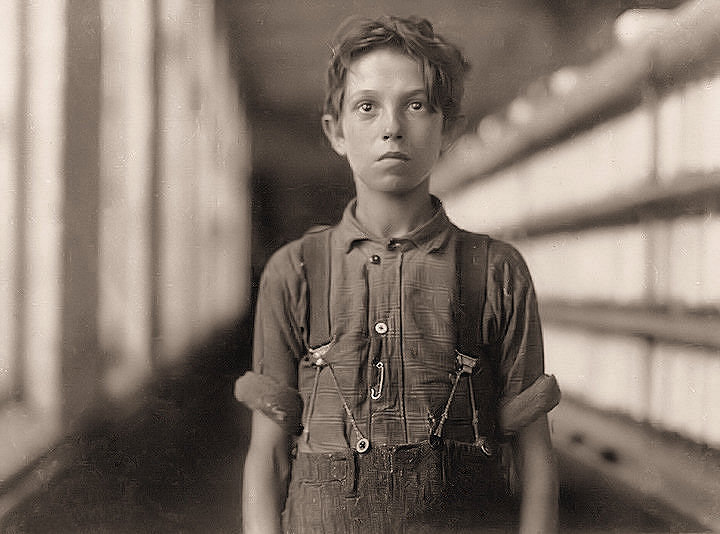
\includegraphics[width=3cm]{hine02}\par
\raggedright
\textit{Cover image: }
The cover image shows Jo Bodeon, a back-roper in the mule room at Chace Cotton Mill. Burlington, Vermont. This and other similar images in this book were taken by Lewis W. Hine, in the period between 1908-1912. These images as well as social campaigns by many including Hine, helped to formulate America's anti-child labour laws.
\end{minipage}\par
\vspace*{\baselineskip}
\begin{minipage}[b]{0.9\textwidth}
\raggedright
\setlength{\parskip}{0.5\baselineskip}
Copyright \copyright 2012  Dr Yiannis Lazarides\par
Permission is granted to copy, distribute and\slash or modify this document under the terms of the GNU Free Documentation License, version 1.2, with no invariant sections, no front-cover texts, and no back-cover texts.\par
A copy of the license is included in the appendix.\par
This document is distributed in the hope that it will be useful, but without any warranty; without even the implied warranty of merchantability or fitness for a particular purpose.
\end{minipage}
\vspace*{2\baselineskip}
\clearpage
}

%% Some special styles
%     \begin{macrocode}
\IfFileExists{changepage.sty}{\RequirePackage{changepage}}{}
\IfFileExists{rotating.sty}{\RequirePackage{rotating}}{}

%    \end{macrocode}
%
% \begin{macro}{\even@samplepage}

% \begin{macro}{\odd@samplepage}
%    \begin{macrocode}
\def\even@samplepage{%
 \begin{picture}(0,0)
   \put(\Xeven,\Yeven){\turnbox{90}{\Huge \textcolor{\watermark@textcolor}{\watermark@text}}}
\end{picture}
}
%% Define a macro to print SAMPLE PAGE IN THE MARGIN
\def\odd@samplepage{%
 \begin{picture}(0,0)
   \put(\Xodd,\Yodd){\turnbox{90}{\Huge \textcolor{\watermark@textcolor}{\watermark@text}}}
 \end{picture}
}
%    \end{macrocode}
% \begin{macro}{watermarktext}
%  Define the watermark words
%    \begin{macrocode}
\def\watermarktext#1{\gdef\watermark@text{\fontfamily{phv}\selectfont#1}}
\def\watermarktextcolor#1{\gdef\watermark@textcolor{#1}}
\watermarktext{SAMPLE PAGE}
\watermarktextcolor{purple}
%    \end{macrocode}
% \end{macro}
%    \begin{macrocode}
%% redefine LaTeX's plain as myplain for headings
\def\ps@samplepage{\let\@mkboth\@gobbletwo
 \let\@oddhead\odd@samplepage\def\@oddfoot{\reset@font\hfil\thepage}
 \let\@evenhead\even@samplepage\def\@evenfoot{\reset@font\thepage\hfil}}
%%
%
%% We define two macros to position the watermark on the page
\def\Xodd{500}
\def\Xeven{-70}\def\Yeven{-810}
\def\Yeven{-\expandafter\strip@pt\textheight}
\let\Yodd\Yeven


\cxset{blank page text/.store in=\blankpagetext@cx{#1}}

\def\cleardoublepage{\clearpage\if@twoside\ifodd\c@page\else
  \hbox{}
  \vspace*{\fill}
  \begin{center}
     \blankpagetext@cx      
  \end{center}
  \vspace{\fill}
  \thispagestyle{empty}
  \newpage
  \if@twocolumn\hbox{}\newpage\fi\fi\fi}

\parindent1.5em

%% Examples for documentation
\newcounter{texexp}[chapter]
\@addtoreset{c@texexp}{c@chapter}
\def\thetexexp{\thesection.\arabic{texexp}}
\tcbset{
texexp/.style={%
   fonttitle=\small\sffamily\bfseries, fontupper=\small, fontlower=\small},
  example/.code 2 args={\refstepcounter{texexp}\label{#2}}%
  \pgfkeysalso{texexp,title={Example \thetexexp\ #1}},
}


\newenvironment{texexp}[1]{\tcblisting{texexp,#1}}{\endtcblisting}
\newenvironment{example}[3][]{\tcblisting{example={#2}{#3},#1}}{\endtcblisting}
%%rename to avoid clashes with other classes that use it

\newenvironment{texexample}[3][]{\tcblisting{example={#2}{#3},#1}}{\endtcblisting}


% Define a macro to hold the name of this package.
\def\athena{\textcolor{thered}{athena}}
% 
% Be nice to hackers define a boolean to know if the package was loaded
\newif\if@athena
\@athenatrue

% STOLEN FROM TUFTE
% \RaggedRight allows hyphenation

\RequirePackage{ragged2e}
\setlength{\RaggedRightRightskip}{\z@ plus 0.08\hsize}
\setlength{\RaggedRightParindent}{1pc}

% Paragraph indentation and separation for normal text
\newcommand{\@tufte@reset@par}{%
  \setlength{\RaggedRightParindent}{1.0pc}%
  \setlength{\parindent}{1pc}%
  \setlength{\parskip}{0pt}%
}
\@tufte@reset@par

% Paragraph indentation and separation for marginal text
\newcommand{\@tufte@margin@par}{%
  \setlength{\RaggedRightParindent}{0.5pc}%
  \setlength{\parindent}{0.5pc}%
  \setlength{\parskip}{0pt}%
}
% Use Donald Arseneau's improved float parameters for the documentation and 
% to develop sensible values.
\renewcommand{\topfraction}{.5}
\renewcommand{\bottomfraction}{.7}
\renewcommand{\textfraction}{.04}
\renewcommand{\floatpagefraction}{.92} % have a high one don't encourage it
\renewcommand{\dbltopfraction}{.66}
\renewcommand{\dblfloatpagefraction}{.66}
\setcounter{topnumber}{9}
\setcounter{bottomnumber}{9}
\setcounter{totalnumber}{20}
\setcounter{dbltopnumber}{9}

% Some people might prefer setting the author fields as macros
\newcommand\addauthors[1]{%
   \cxset{author names=#1}
}

%%%%%%%%%%%%% CHAPTERS %%%%%%%%%%%%%%%%%%%%%%%%%%%%%%
\cxset{custom/.code=\gdef\customdesign@cx{\csname#1\endcsname}\@specialtrue,
       fill/.store in=\fill@cx}
%\cxset{stefan/.style={fill=purple, title font-color=\color{white},
%          custom=tikzspecials}}


\cxset{steward/.style={
  offsety/.store in=\soffsety,
  image/.store in=\image@cx,
  texti/.store in=\texti@cx,
  textii/.store in=\textii@cx,
  header style=empty,
}}


\newcommand\tikzspecial[2][]{%
     \clearpage

     \begin{tikzpicture}[remember picture,overlay]
     % Main shading block
     \node [xshift=5cm,yshift=-\paperheight] at (current page.north west)
        [text width=0.98\textwidth,text height=\paperheight, fill=thecream!30,rounded corners,above right]
        {};
      \node [xshift=6.5cm,yshift=-1.5cm-\soffsety] at (current page.north west)
         [text width=0.7\textwidth,below right]{\sffamily \bfseries \huge\raggedright #2\par};

        \node [xshift=3cm,yshift=-1.5cm] at (current page.north west)
      [text width=3cm,align=center,minimum height=2.5cm, fill=blue,below right]
	{$$\text{\HHUGE\bfseries\sffamily\color{white}\thechapter}$$
	\par\vspace*{3pt}
	};

	\node [xshift=-0.2cm,yshift=-21.5cm] at (current page.north west)
	[text width=3cm,above right]%
	{\includegraphics[width=1.0\paperwidth]{./chapters/\image@cx}};
	% second box left
	\node [xshift=3cm,yshift=-19.5cm] at (current page.north west)
	[text width=9cm,minimum height=2.5cm,inner sep=0.5em, fill=blue,below right]
	{\color{white}
 	 \bfseries\sffamily \texti@cx
	};
	% Last block
	\node [xshift=6.5cm,yshift=-26cm] at (current page.north west)
	[text width=12cm,above right]
	{\textii@cx};
	\end{tikzpicture}
\par
\thispagestyle{empty}
\clearpage
}%end tikzspecial

\cxset{steward,
  chapter toc=true,
  numbering=arabic,
  custom=tikzspecial,
  offsety=0cm,
  image=hine03,
  texti={Type some text here by setting texti},
  textii={Type some text here by setting textii},
 }


%% EDDOUARD MANET

\cxset{manet/.style={
 chapter opening=anywhere,
 chapter toc=true,
 toc image=false,
 name={},
 numbering=none,
 number font-size=,
 number font-family=,
 number font-weight=,
 number before={\vspace*{-2.5cm}},
 number dot={},
 number after={},
 number position=leftname,
 chapter font-family=,
 chapter font-weight=,
 chapter font-size=,
 chapter before={},
 chapter after={},
 chapter color={black!90},
 number color=\color{purple},
 title beforeskip={},
 title afterskip={},
 title before={\hskip-2.3cm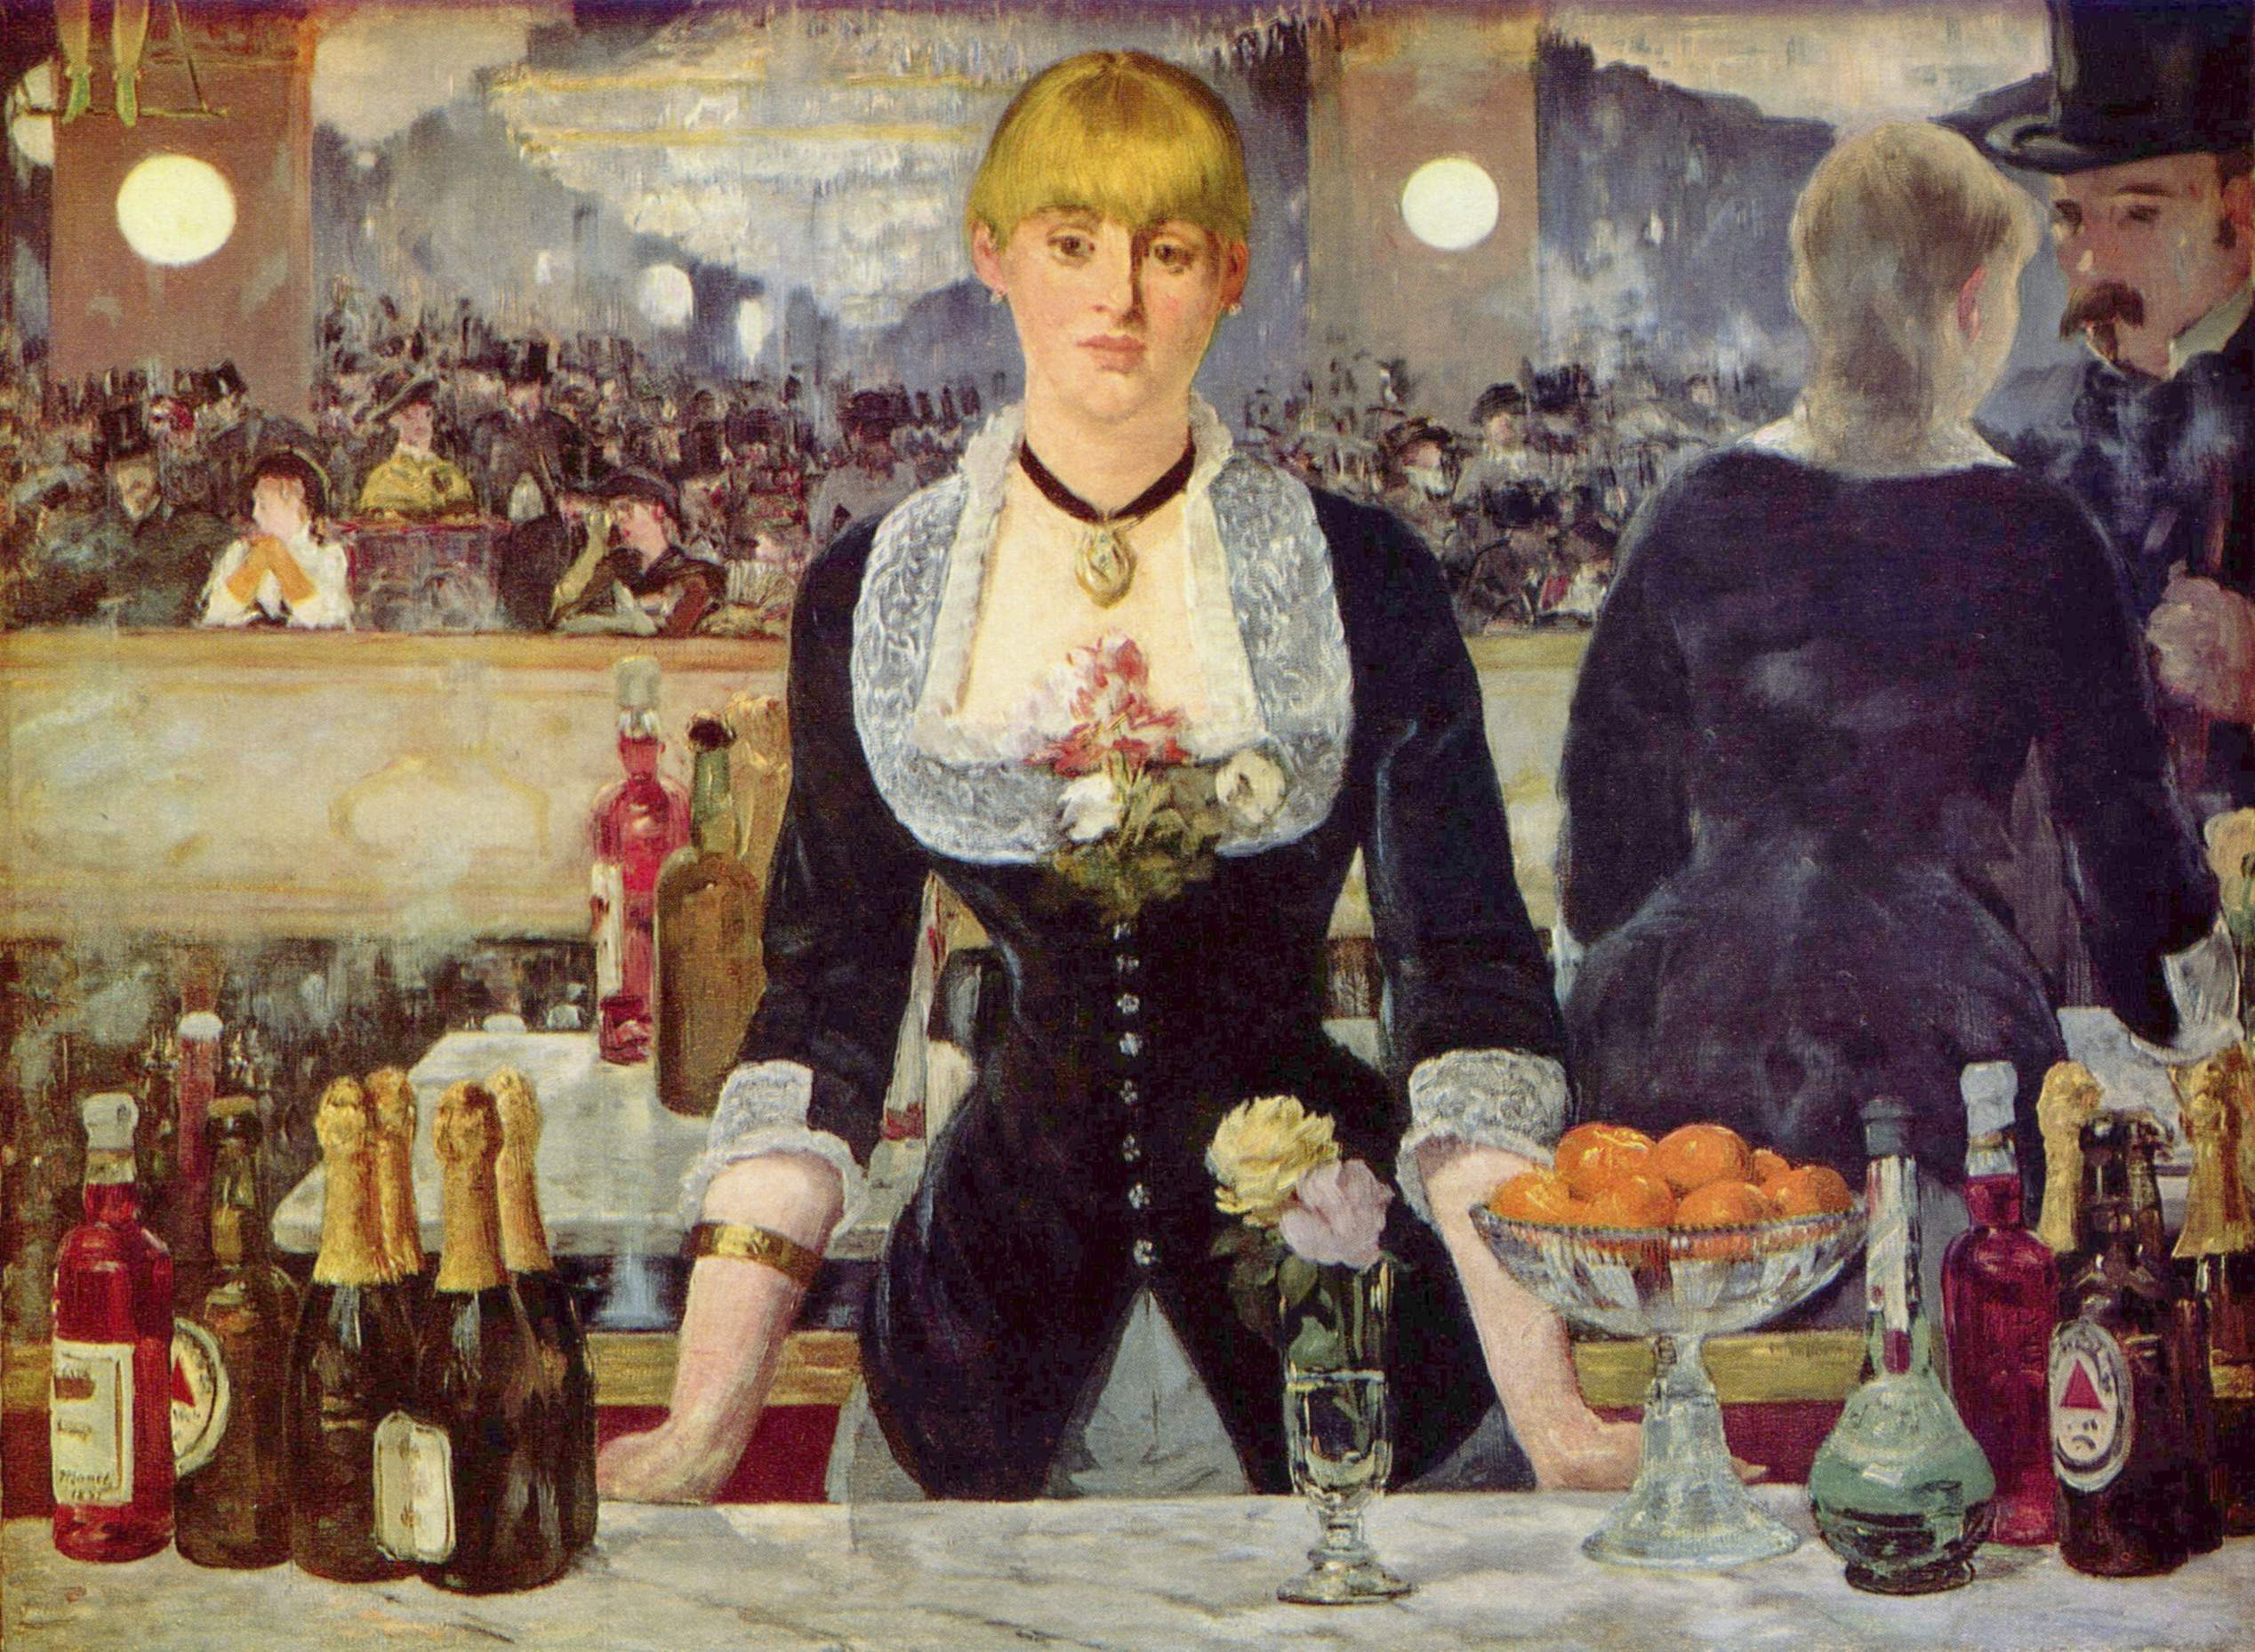
\includegraphics[width=1.25\textwidth]{./chapters/manet}\par
    \par\hfill\hfill{\tiny\bfseries Manet's  \textit{The Barmaid.}}\\
    \par
    \vspace*{\baselineskip}
    \par\hfill},
 title after={\hfill\hfill},
 title font-family=\sffamily,
 title font-color=\color{black!80},
 title font-weight=\bfseries,
 title font-size=\LARGE,
 header style=plain}}

\def\topimage#1{\cxset{title before={\vspace*{\headsep}\hspace*{\dimexpr(-\marginparwidth-2.1cm-\marginparsep)}\includegraphics[width=\paperwidth]{./chapters/#1}\par
\vspace*{\baselineskip}\par}}}
% need to reset 
\cxset{manet, toc image=true}
\begin{document}


\frontmatter
\pagestyle{empty}
%\coverpage{hine02}{Yiannis Lazarides}{Published by Camel Press}savinggrace,vespa

\coverpage{bird-brain}{Yiannis Lazarides}{Published by Camel Press}
\secondpage
\thispagestyle{samplepage}
%% temporary titles
% command to provide stretchy vertical space in proportion
\newcommand\nbvspace[1][1]{\vspace*{\stretch{#1}}}
% allow some slack to avoid under/overfull boxes
\newcommand\nbstretchyspace{\spaceskip0.5em plus 0.25em minus 0.25em}
% To improve spacing on titlepages
\newcommand{\nbtitlestretch}{\spaceskip0.6em}
\pagestyle{empty}
\begin{center}
\bfseries
\nbvspace[1]
\Huge
{\nbtitlestretch\huge
A NEW LOOK AT\\ LATEX BOOK DESIGN}

\nbvspace[1]
\normalsize

TO WHICH IS ADDED MANY USEFUL MACROS\\
AND THE \textbf{CHAPTERX} PACKAGE SO THAT\\
YOU CAN MAKE BEAUTIFUL BOOKS\\
%YOU CAN CODE LIKE A HAWK
\nbvspace[1]
\small BY\\
\Large DR YIANNIS LAZARIDES\\[0.5em]
%\footnotesize AUTHOR OF ``A WORKING ALGEBRA,'' ``WIRELESS TELEGRAPHY,\\
%ITS HISTORY, THEORY AND PRACTICE,'' ETC., ETC.

\nbvspace[2]

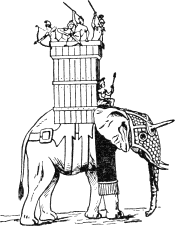
\includegraphics[width=1.5in]{pic37}
\nbvspace[3]
\normalsize

DOHA\\
\large
PUBLISHED IN THE WILD
\nbvspace[1]
\end{center}

% Must move from here
\cxset{blank page text=\epigraph{We all agree that your theory is crazy. 
          But is it crazy enough?}{Niels Bohr}}

%%%%%%%%%%%  MAIN MATTER %%%%%%%%%%%%%%%%%%%%%%%%%%%%%%
\mainmatter

\pagestyle{plain}
\@specialfalse
\tableofcontents
\listoftables
\listoffigures


\cxset{toc image=true}
\part{The Package}


\pagestyle{plain}
\setdefaults

% eatern!!

\makeatletter\@specialfalse\@debugfalse\makeatother
\cxset{style13}
\cxset{title margin bottom=10pt}
\chapter{Introduction}
\addtocimage{-12pt}{-20pt}{../images/tocblock-fish.jpg}


\epigraph{``Begin at the beginning,'' the king said
"and then go on till you come to the end, then stop."}{
---Lewis Carroll, Alice in Wonderland}

\large

\noindent This package and its documentation attempts to eliminate some common 
problems encountered when using \LaTeX2e. The first one is the loading of 
recommended packages for a large and perhaps complicated document and 
the second is the re-designing of styles for a document.

 \LaTeX2e, does not provide a standard library, but comes equipped with
 a package mechanism that allows code extensions to be loaded as required.
 This has created a strong vibrant community, hundreds of packages and a 
 headache to both new and seasoned users. What packages are available, when
 to use them and in which order is a common theme for many questions on
 lists and |TX.SE|.

 It is quite common during the writing of a thesis or book
 for the author to keep on adding macros and packages
 at the preamble of the document. In most cases this can
 be satisfactory but in many others it leads to
 incompatibilities and errors. This package aims at
 minimizing one's preamble, by prefetching a number of
 commonly used packages. It also aims at loading them
 in the right order and providing patches for conflicts.
 
 I am hoping that using this package, will lead to less
 frustrations with the intricacies of \LaTeX2e\ packages.

The package code is complicated, but its usage is simple. You first load the package and then
you use one of the available templates:

 \begin{commands}[]{}
 \begin{verbatim}
 \usepackage{phd}
 \usetemplate{style13}
 \end{verbatim}
 \end{commands}

This is what you need to typeset a good looking book or thesis. The rest of this book is a footnote and you can skip them if you want. 

It will be better for the longer projects to just fork the
 package and adapt it to your needs. In this respect, I have
 uploaded the package to |github|.\footnote{\url{https://github.com/yannisl/phd}}

 My goal in selecting the packages and adding a number of 
 commands for the authors was to be able to typeset a 
 document for most common use cases, without the need of
 additional packages. The packages I selected are biased
 towards academic publications, although they can find use
 in almost any fields. The package provides a mechanism via
 PGF keys to provide a settings file. 
 
 Most of the documentation can be found in the implementation part.

Browse any books in a library or bookshop and the striking thing is that their design is very individualistic. They might have similarities but their main features vary. In many respects they resemble people's faces where minor differences have striking effects.

This package arose out of a question at stackexchange. How to redefine chapter heads. Having seen the popularity of the |pgf| package \cite{pkg-pgf} I realized that \latex users prefer this method of styling rather the traditional \latex method.

The user interface can be extended to basically all major packages. The principle is to keep to a minimum changes that can affect the LaTeX core commands. If there are any additions a key setting is provided to be able to revert back to normal LaTeX.

The workflow can be simplified. In addition I want to believe that the interface can provide a useful addition to the open source community and that other people will contribute style libraries, which will be simpler to write. It is also possible
to device an easy and uncomplicated web interface to handle
such a great number of variables.


Most people when they get started with \LaTeX\ will either use one of the standard classes such as the \docfile{book.cls} or one of the generic classes notably koma-script or memoir. Most students will be forced to use on of the many thesis classes available.

\section{The key value concept}

The key-value concept that originated with \LaTeX\ has been extended many times, the last and most serious implementation of it by Tantau in the PGF package. What essentially Tantau developed is a scripting language to script TeX code. The \tikzname and pgfplots packages are two major packaged that use keys effectively. Their popularity is growing and what this package does is to offer a user interface that has been modelled to be similar to that of \texttt{css} (cascade style sheets). 
\smallskip

\begin{scriptexample}{}{}
\textit{number} font-size = Large,\\
\textit{chapter} color = theblue
\end{scriptexample}
\smallskip

The main idea behind the package, is that you are configuring a document style by means of \emph{settings} rather than writing macros. In the example above the \emph{number, chapter} can be thought of as class or id names in css style sheets and the |font-size, color| as property settings that apply to the particular element. 


\subsection{Settings}

Settings are activated either by using the command |\cxset|  or by loading a full style sheet. In most cases you will probably import a style sheet and then modify some of the properties using |cxset|.  For example this heading has a dot after the subsection number. This was accomplished by setting,

We can de-activate it for the next and subsequent subsection headings with the setting:

\begin{scriptexample}{}{}
\begin{verbatim}
\cxset{subsection number after=\quad}
\end{verbatim}
\end{scriptexample}


\cxset{subsection number after=\quad,
          section number after=\quad,
          title margin bottom=10pt}
\renewsubsection

\subsection{Cascading}

Most values once set for a higher section will be seen in a cascade by all subsectioning commands in a similar fashion similar to CSS. These include properties such as color, font families and alignment. Best though to specify all of them for maximum flexibility to your users.

\section{On typography}

This package hopefully will assist in improving the typography of books set with \latexe. Any typographical comments on the various styles are just my own ramblingss and not necessarily absolute truths. Like fashion and art typography has opinions rather than absolute truths. In many styles the design is slightly adapted to blend a bit better with this manual. Also I did not select fonts as per the samples but this is left on you the user to decide.



\section{Packages and Fonts}

This manual has been typeset with numerous fonts in order to enable the typsetting of almost all the scripts provided by the Unicode standard. In order to process it from the |.dtx| file, these fonts must be available in your system, otherwise \XeLaTeX\ will have a problem finding the fonts and it will take an awful long time to process. This is especially true for the scripts section, where virtually all the Unicode defined scripts are discussed. You will need a fast computer and a fast hard disk to process the document within a reasonable time. When using \pkgname{fontspec} always define your fonts with the \cmd{\newfontfamily} this will speed up processing by an order of magnitude. Compiling from the command prompt will speed up compilation. Average speed 2-3 pages per second.

Many of \tex's parameters are stretched to the limit with a complicated document such as this manual. You will require a full distribution otherwise expect some errors. Important packages is \pkgname{morefloats} and \pkgname{morewrites}. The package will also expect that you have |e-tex| installed. Ubuntu users are normally one year behind in updates, so you might wish to update manually. It will take upwards of 5 minutes to compile fully on an old laptop and a couple of minutes on a state of the art computer.

The |dtx| should be processed best with its own make file provided for Windows only |phd.bat|. The make file will process the documentation using \lualatex. You can also process the document with \xelatex but is prone to produce errors. Using \latexe the sections on scripts etc will not be printed and a much shorter version of the manual is provided. 

\section{Scripts and Languages}

The package and the documentation offer a full repertoire of font selection keys for different scripts and languages. It hasn't been possible, however hard I tried to compile this section of the documentation with \xelatex, as it kept giving errors of too many files open. This was also not possible even with the \pkgname{morewrites} package loaded. With \lualatex the document compiled with no major problems other than the font rendering being of a lower quality to that of XeLaTeX om windows, other than disabling incompatible packages and a number of commands that were redefined. 

Some good news for multi-script typesetting is the Noto fonts from Google. These fonts named Noto from "No Tofu" meaning you do not see any little square blocks for undefined glyphs, are fast to load. Disantvantage you need to switch between font commands fairly often.

\section{This manual}

When developing the templates, I started using \emph{lorem ipsum} text as samples. Half-way through this
became a jumble mass of uninteresting pages interspersed with code. Headings and the contents of the book
determine both the structure and the selection of fonts, so I went back and wrote narratives  to accompany
the headings. Many of the narratives are semi-autobiographical in nature; others are clustered around books I read and my own interests. Some I stumbled on them accidentally and are mostly there to demonstrate some code.

Besides the templates and the code there is another narrative which is based on notes I kept on \tex and its friends over the years and are offered as a more advanced introduction to coding \latexe and \tex. The whole manual was typeset in a |ltxdoc| class, slightly modified to turn into a book class.

The implementation code is also available and it was mostly for my own benefit. The whole manual with the exception of the |\cxset| introduction, is just a test document. The notes and the “dissection” of the standard \latexe and the standard classes are there to explain the background to the many coding decisions that I took while I was developing the package.

PhD students are notorious for going in all directions and exploring many adjacent fields before they sit down and write their theses. Some become life-time students. To all these new men and women of the Renaissance that slave away to inch knowledge one thesis at a time, I dedicate this book and the name of the package.

 \section{Version control with Git and Github}
 
 If you are involved with code or a publication that will have frequent changes, you should consider
 some type of version control system. My own recommendation is to use |git| and an online repository such
 as |github|. The latter is currently very fashionable and makes sharing code easier. Note that the |github|
 offers both public as well as private repositories. The general recommendation is that for unpublished work
 such as a thesis or code under development, it is preferable to go for a private repository. 
 

 \section{Ordering of Packages}
 
One package that normally leads to errors is the 
\pkgname{hyperref}. The package which is an outstanding example of software engineering and supported single handledy by Heiko Oberdiek \citeyearpar{hyperref} redefines a a lot of internal commands of the kernel. As a lot of other packages do the same it has to be loaded at the end of the preable with the exception of some packages! 
 
 This manual is typeset according to the conventions of the
 \LaTeX \textsc{docstrip} utility which enables the automatic
 extraction of the \LaTeX{} macro source files~\cite{GOOSSENS94}.

 
 \href{http://tex.stackexchange.com/questions/96350/problem-with-algorithmic-and-hyperref}{problem with algorithmic and hyperref}

 \begin{verbatim}
\usepackage{float}  % load float package first!

\usepackage{hyperref} % let hyperref patch the float package stuff
.
 \usepackage{algorithm} % let algorithm use the patched version of the float package
 \end{verbatim}
 

\section{Known problems}

Perhaps the biggest issue with the package is the speed of
compilation with \XeLaTeX\ or \LuaTeX. This is to be expected, as both engines spend a lot of resources in font management. On demand loading of packages is something I have in the back of my mind. This should be done via document styles i.e., if a book is for the humanities, perhaps only a rudimentary amount of maths packages should be loaded.

\section{Future Directions}

\latexe and \tex usage appears to be increasing. This is mostly by programs that export results with \latexe code rather than authors writing books.  The method adopted here is easier to automate all sorts of reports and automated texts. I would like too develop a web interface for processing such templates and at the same time export into html instead of just producing pdfs. I have already a prototype.   

%\ClockFramefalse\ClockStyle=0\clock{13}{10}
%\ClockFramefalse\ClockStyle=1\clock{14}{22}
%\ClockFramefalse\ClockStyle=2\clock{15}{48}
%\ClockFramefalse\ClockStyle=3\clock{7}{50}
%
%\ClockFrametrue\ClockStyle=0\clock{11}{32}
%\ClockFrametrue\ClockStyle=1\clock{12}{0}
%\ClockFrametrue\ClockStyle=2\clock{8}{9}
%\ClockFrametrue\ClockStyle=3\clock{1}{15}

{\HHHUGE\showclock{0}{45}}












\makeatletter
\cxset{toc image=\@empty}

\@specialtrue
\setdefaults 
\renewcommand\stewart[2][]{%
\fancypagestyle{fancy}{%
\lhead{}\rhead{}
\chead{}
\cfoot{}
\lfoot{}
\rfoot{\thepage}
\def\footrule#1{{\color{blue}%
  \hrule width\paperwidth}\vskip3pt
}

\renewcommand{\headrulewidth}{0pt}
\renewcommand{\footrulewidth}{0.4pt}}

\clearpage

\begin{tikzpicture}[remember picture,overlay]
% Main shading block
\node [xshift=5cm,yshift=-\paperheight] at (current page.north west)
[text width=0.98\textwidth,text height=\paperheight, fill=thecream!30,rounded corners,above right]
{};
\node [xshift=6.5cm,yshift=-1.5cm-\soffsety] at (current page.north west)
[text width=0.9\textwidth,below right]{\sffamily \bfseries \huge #2};

\node [xshift=3cm,yshift=-1.5cm] at (current page.north west)
[text width=3cm,align=center,minimum height=2.5cm, fill=blue,below right]
{\[\text{\HHUGE\bfseries\sffamily\color{white}\thechapter}\]
\par\vspace*{3pt}
};

\node [xshift=-0.2cm,yshift=-21.5cm] at (current page.north west)
[text width=3cm,above right]%
{\includegraphics[width=1.0\paperwidth]{./chapters/\image@cx}};
% second box left
\node [xshift=3cm,yshift=-19.5cm] at (current page.north west)
[text width=9cm,minimum height=2.5cm,inner sep=0.5em, fill=blue,below right]
{\color{white}
  \bfseries\sffamily \texti@cx
};
% Last block
\node [xshift=6.5cm,yshift=-26cm] at (current page.north west)
[text width=12cm,above right]
{\textii@cx
};
\end{tikzpicture}
\par
\clearpage
}





\cxset{steward,
  numbering=arabic,
  custom=stewart,
  offsety=0cm,
  image=hine03,
  texti={When Lamport designed the original \LaTeX\ sectioning commands he did not provide a fully comprehensive interface for modifying their design. With current tools available improvements are much easier to program and this chapter provides the details.},
  textii={\precis{In this chapter we discuss a method that allows the production of fancy chapter headings and formatting, based on a set of key values. Central  to this process is the separation of content from presentation.
We also discuss the basic formatting tools that are available and how one can modify them to mould new book designs.}
 }
}


\chapter{Designing Chapters}

\section{Introduction}

For too long, the act of printing something in and of itself has been placed on too high a pedestal. The true value of an object lies in what it says, not its mere existence. And in the case of a book, that value is intrinsically connected to content. The aim of this package is to try and provide a bridge between separating content from presentation.

A new chapter must make a good impression and must give an immediate signal that something different is going to be written. Traditionally chapter openings in LaTeX are an unimpressive and dry event. Our aim is to brighten it up a bit, while keeping true separation of content from presentation.



\section{Package Usage}

To use the package include it just like any other package:

\begin{tcolorbox}
\begin{lstlisting}
\documentclass{book}
\usepackage{chaptersx}
\cxset{style13}
\begin{document}
\chapter{Introduction}
\end{document}
\end{lstlisting}
\end{tcolorbox}

The command \cs{cxset} sets the default style for the example to the style defined as \marg{style13}. The package currently offers over 50 styles and numerous keys to manipulate them further.



\section{Chapter opening page}

The standard LaTeX classes offer only two options to either open a chapter on an odd page or at any page. This package offers five alternatives:

\keyval{chapter opening}{\marg{any, left, right, anywhere, ifafter}}{The various keys enable any combination to be used.}

\begin{marglist}
\item [any] Opens a chapter at any page, either verso or recto.
\item [left] Opens a chapter on an even page
\item [right] Opens a chapter on a right page.
\item [anywhere] Opens a chapter at the point where the \cs{chapter} is typed.
\item [none] Alias for \marg{anywhere}.
\item [ifafter] Opens a chapter at the next page if the page has material that does not exceed a certain portion of \cs{textheight}.
\end{marglist}

To change a setting you just modify the value of the key \option{chapter opening} to one of the values described earlier.

\begin{tcolorbox}
\begin{lstlisting}
\cxset{chapter opening=anywhere}
\end{lstlisting}
\end{tcolorbox}

\@specialfalse
\cxset{chapter toc=false}
\begin{texexample}{title=Inline Chapter Example}{ex:anywhere}
\cxset{chapter opening=anywhere, chapter before=\bigskip, chapter font-family=\sffamily,title font-family=\sffamily}

\lipsum[2]
\chapter{Chapter Example}
\lipsum[3]
\chapter{Another Chapter Example}
\lipsum[4]
\end{texexample}



\addtocounter{chapter}{-1}

Examples for other types of chapter openings follow in the rest of the documentation.

\subsection{Blank pages before chapters}
In the standard LaTeX book class when the openany option is not given or in the report class when the openright is given, chapters start at odd-numbered pages. This can cause a blank page to be printed. Some book designers prefer this page to be completely empty, without any headers or footers. This cannot be done with \lstinline{\thispagestyle} as this command will have to be issued on the \textit{previous} page. However by a suitable redefinition of the
\lstinline{\clearpage} this can be done automatically.
\medskip

\begin{tcolorbox}
\begin{lstlisting}
\makeatletter
\def\cleardoublepage{\clearpage\if@twoside\ifodd\c@page\else
  \hbox{}
  \vspace*{\fill}
  \begin{center}
    This page left intentionally blank.
  \end{center}
  \vspace{\fill}
  \thispagestyle{empty}
  \newpage
  \if@twocolumn\hbox{}\newpage\fi\fi\fi}
\makeatother
\end{lstlisting}
\end{tcolorbox}
\medskip

This is achieved easily by setting the following options:
\bigskip

\begin{tcolorbox}
\lstinline{chapter blank page=empty}\par
\lstinline{chapter blank page text=Some text.}\par
\lstinline{chapter blank page=plain}\par
\end{tcolorbox}
\medskip



The last one refers to a \lstinline!\thispagestyle{plain}!.

\section{Keys for chapter head formatting}

A chapter heading can be considered of being constructed of several parts, the \textit{chapter number}, the chapter name typically \textit{chapter} and the \textit{title}. Predefined keys handle all the elements of formatting. Additional keys are defined to handle other elements such as inclusion of images or producing complicated examples with graphics constructed with TikZ or other similar packages.

\medskip

\keyval{chapter numbering font-size}{\oarg{sizing commands}}{}.
\keyval{chapter numbering font-family}{\oarg{sizing commands}}{}.

\subsection{Keys for numbering}
Chapter numbering follows that of the standard \LaTeX\ classes and is extended to cover some additional cases such as fully spelled out numbers.

\keyval{number numbering}{\oarg{alph,Alph,roman,Roman,none,WORDS,words}}{Style of numbering.}
\medskip

\parindent1.5em

Note that the package uses Heiko Oberdiek's package alphalph to allow for alphabetic numbering that extends beyond the normal 26 letters of the alphabet. Examples for numbering can be seen in \ref{ex:romannumbering}

\medskip




\begin{marglist}
\item [arabic] Despite that the Arabs call what the West calls Arabic numbers Indian numbers, we provide the value arabic to have normal numbers printed.
\item [alph] Lowercase alphabetic numbering.
\item [Alph] Uppercase alphabetic numbering.
\item [roman] Lowercase roman numbering.
\item [Roman] Uppercase roman numbering.
\item [words]
\item [WORDS]
\item [Words] Prints the number in words and capitalizes the first letter, for example the number 21 will be printed as `Twenty One'\footnote{Currently limited to the first hundred numbers}.
\item [none] This is equivalent to using the star version of the command. It does not print any number and does not increment the chapter counter.\footnote{I am ambivalent about this, perhaps it will be better to increment it, as it can give a more general approach.}
\end{marglist}

\cxset{chapter opening=anywhere, numbering=Roman}
\index{chapter design!numbering!roman}
\begin{texexample}{Setting up keys for numbering}{ex:romannumbering}
\cxset{numbering=Roman}
\chapter{Roman numbering}
\end{texexample}



\clearpage

\index{chapter design!numbering!words}
\begin{texexample}{title=Chapter number in words}{}
\cxset{numbering=WORDS}
\chapter{Literal numbering}
\end{texexample}



\cxset{numbering=arabic}
\subsection{Setting font information}
\subsection{Letter spacing}

Chapter letter spacing can be achieved using the soul package in a combination with the key spaceout.
\medskip



\keyval{chapter spaceout}{\marg{soul}}{Uses the soul package to space out the lettering of chapter, number or the chapter name.}\par\medskip



The following examples illustrate the usage.

\begin{texexample}{}{}
\cxset{numbering=Roman,
         chapter spaceout=none,
         title spaceout=soul,
         title font-size=\Large,
         title font-family=\rmfamily,
         title font-shape=\scshape}
\chapter{Letter Spacing}
\end{texexample}



\index{chapter design!labels!letter spacing}
\begin{texexample}{}{} 
\cxset{chapter spaceout=soul,numbering=arabic, title spaceout=soul}
\chapter{Chapter title}
\end{texexample}



\subsection{Styling the title}

Similarly to the number and chapter styling keys exist for styling the title. We summarize the available standard keys below:
\medskip

  \keyval{chapter title font-family}{\marg{family}}{Selects a predefined font family}
  \keyval{chapter title font-weight}{\marg{\cs{bfseries},\cs{normalseries}}}{Font weight.}
  \keyval{chapter title font-size}{\marg{\cs{large},\cs{Large},\cs{huge},\cs{Huge},\cs{HUGE},\cs{HHuge}}}{Font sizing command.}
  \keyval{chapter title font-color}{}{}
  \keyval{chapter title spaceout}{\marg{soul,none}}{}
  \keyval{title before}{}{}
 \keyval{title after}{}{}
  \keyval{title beforeskip}{}{}
  \keyval{title afterskip}{}{}


\begin{texexample}{letter spacing the chapter title block}{}
\cxset{style13, chapter spaceout=none,
       numbering=arabic}
\chapter{Chapter Title Styling}
\end{texexample}



The last example illustrated the use of a predefined style \oarg{style13} and overriding some of the parameters.


\cxset{chapter opening=right}
\section{Table of Contents}\index{table of contents!key settings}

Traditionally a chapter will be added to the Table of Contents if the \cs{chapter} command is issued. The starred version will not produce a number and will not add a contents line. Since we have adopted an approach where we use a key value interface we can dispense with the starred version of the command, by setting the \option{chapter toc} option to false. For example if we want to define a command for a ``Foreward'' or ``Epiloque'' without wishing them to be added to the table of contents we can use the following setting.\index{Foreward!definitions}\index{Epilogue!definitions}



\begin{texexample}{changing the chapter label name}{}
\cxset{chapter toc=false, name=, numbering=none,}
\chapter{Foreward}
\lorem
\end{texexample}

Note that the key \option{numbering=none} still has to be set.


Please note that when \textbf{numbering=none} the chapter number is not available anymore and yo may have to reset it if required again. Although this might be seen as rather cumbersome than simply using \cs{chapter*} the advantage is consistency in the user interface and the use of appropriate semantic definitions for all sectioning commands thus achieving a bit more separation of context from style.


\cxset{chapter toc=true}

\section{Defining styles}

Named styles can be defined using the standard \textsc{PGF} conventions. To define a style for the forward above we can use:

\begin{texexample}{}{}
\cxset{foreward/.style={chapter toc=false,numbering=none,
          name=,
          title font-size= Large,
          title font-family= sffamily,
          numbering=none}}
\cxset{foreward}
\chapter{Foreward.}
\lorem
\end{texexample}



\cxset{numbering=arabic}
\section{Creating semantic names for commands and environments}

To keep our search for semantic commands and true separation of contents it is prudent to define some macros for typesetting the  `foreward' section.

\begin{texexample}{defining a \textit{Foreward} macro.}{}
\begin{lstlisting}
\cxset{foreward/.style={chapter toc=false,
          name=,
          title font-size = Large,
          title font-family = sffamily,
          numbering=none}}
\newcommand\forewardname{foreward}
\expandafter\newenvironment\expandafter{\forewardname}{%
\cxset{foreward}\chapter{Foreward}}%
{}
\begin{foreward}
\lorem
\end{foreward}
\end{lstlisting}
\end{texexample}



Notice the use of a new command \cs{forewardname} to allow for internationlization using Babel or other methods. One is tempted to let the English name, but a better approach perhaps is to define both.



\@specialtrue
\cxset{steward,
  numbering=arabic,
  custom=stewart,
  offsety=0cm,
  image=hine03,
  texti={When Lamport designed the original \LaTeX\ sectioning commands he did not provide a fully comprehensive interface for modifying their design. With current tools available improvements are much easier to program and this chapter provides the details.},
%
  textii={In this chapter we discuss a method that allows the production of fancy chapter headings and formatting, based on a set of key values. Central  to this process is the separation of content from presentation.
We also discuss the basic formatting tools that are available and how one can modify them to mould new book designs.
 },
 pagestyle = empty
}



\chapter{Setting up Fonts}

\section{Introduction}

Selecting the right fonts for a book is the job of the book designer. For people using pdfLaTeX this is rather limiting and I would highly recommend for any serious typesetting work to move onto XeLaTeX.

One of the things we need to take care of, is to ensure that the document compiles irrespective of the \TeX\ engine used. I suggest code similar to that shown in the example below that enables loading of main fonts based on the \TeX\ engine.

\begin{tcolorbox}
\begin{lstlisting}
\usepackage{ifxetex}
\ifxetex
  \usepackage{fontspec}
  \defaultfontfeatures{Mapping=tex-text}
  \setmainfont{Times New Roman}
  \setsansfont{Myriad Pro}
\else
  \usepackage{lmodern}
  \usepackage[T1]{fontenc}
\fi
\end{lstlisting}
\end{tcolorbox}

For free fonts there exist a few resources that can be used with \LaTeX.
\url{http://tex.stackexchange.com/questions/53416/using-a-good-non-default-font}. Integrating them within a new document can be a nightmare but is the job of the class and book designer.

\section{Terminology}

The best source of information for XeTeX is the fontspec manual. It is not an easy read, but if you are going to be resetting a lot of fonts, it is advisable to do so.

Most typesetting systems allow for setting document wide fonts. In LaTeX we get the following commands:


\cs{sffamily}

\cs{rmfamily}

\cs{ttfamily}

To be able to use \athena\ properly you will have to familiarize yourself with the terminology, if you are not.

CSS uses a combination of font-family and fallback generic families to achieve this and it is instructive to review it as we will use such a system here.

\begin{tcolorbox}
\begin{lstlisting}
p{font-family:"Times New Roman",Georgia,Serif;}
\end{lstlisting}
\end{tcolorbox}

The font-family property specifies the font for an element.

The font-family property can hold several font names as a "fallback" system. If the browser does not support the first font, it tries the next font.

There are two types of font family names:

family-name - The name of a font-family, like "times", "courier", "arial", etc.

generic-family - The name of a generic-family, like "serif", "sans-serif", "cursive", "fantasy", "monospace".

There is though a fundamental difference that one needs to keep in mind, \TeX\ exists in order to always typeset the same on any machine. CSS endeavours to run in any browser and any system, disregarding typography. Nevertheless I decided to provide the interface so at least as to enable document compilation at all times, well almost all times.


\section{General font selection with fontspec}

\begin{trivlist}
\item [\cs{fontspec}\oarg{font features}\marg{font name}]
\item [\cs{setmainfont}\oarg{font features}\marg{font name}]
\item [\cs{setsansfont}\oarg{font features}\marg{font name}]
\item [\cs{setmonofont}\oarg{font features}\marg{font name}]
\item [\cs{newfontfamily}\marg{cmd}\oarg{font features}\marg{font name}]
\end{trivlist}

These are the main font-selecting commands of this package. The \cs{fontspec}
command selects a font for one-time use; all others should be used to define the
standard fonts used in a document. They will be described later in this section.
The font features argument accepts comma separated \marg{font feature}=\marg{option}
lists; these are described in later:

\ifxetex
\begin{texexample}{}{}
\fontspec{Verdana}
\raggedright
\lorem
\end{texexample}
\fi


\subsection{Setting font features}

The fontspec package enables the selection of font features during run-time; font features are items such as colors, proportional OldStyle numbers and other similar items. Some of the examples that follow have been extracted from the fontspec documentation.

\ifxetex
\begin{texexample}{}{}
\fontspec[Numbers={Proportional,OldStyle}]
{TeX Gyre Adventor}
`In 1842, 999 people sailed 97 miles in
13 boats. In 1923, 111 people sailed 54
miles in 56 boats.' \bigskip

\fontspec{TeX Gyre Adventor}
`In 1842, 999 people sailed 97 miles in
13 boats. In 1923, 111 people sailed 54
miles in 56 boats.' \bigskip
\end{texexample}
\fi


\section{The \athena\ package interface.}

By design feature options for XeTeX/XeLaTeX have currently bee restricted. The reason behind this decision is that I was concerned that I would have added a complicated interface with very little reason as to its use. I opted for a more semantic approach and expect the user to define custom macros to handle anything else.
\medskip

\keyval{mainfont}{\marg{font1,font2,font3}}{A comma separated list of one or more font-names. The main font will be set to the first font found.}
\keyval{chapterfont}{\marg{font1,font2,font3}}{A comma separated list of one or more font-names. The main font will be set to the first font found.}
\keyval{sectionfont}{\marg{font1,font2,font3}}{A comma separated list of one or more font-names. The main font will be set to the first font found.}
\keyval{contentsfont}{\marg{font1,font2,font3}}{A comma separated list of one or more font-names. The main font will be set to the first font found.}
\keyval{bibliographyfont}{\marg{font1,font2,font3}}{A comma separated list of one or more font-names. The main font will be set to the first font found.}

Note that the package will first check if is running under XeTeX. If it does it will execute the commands and load the macros, otherwise it will fall back on pdfLaTeX commands.

\section{Discussion}


Unfortunately, even with the best will loading fonts will always be a difficult task in TeX. Hopefully the interface provided will result in better separation of presentation from content and offers consistency in the styling of documents. Nothing prevents you from adding normal macros to styles. Each style can be treated as a package in many respects.








\makeatletter\@specialfalse
\cxset{custom = stewart}
\cxset{steward,
  numbering=arabic,
  custom=stewart,
  offsety=0cm,
  image={./images/hine03.jpg},
  texti={When Lamport designed the original \LaTeX\ sectioning commands he did not provide a fully comprehensive interface for modifying their design. With current tools available improvements are much easier to program and this chapter provides the details.},
  textii={\precis{In this chapter we discuss a method that allows the production of fancy chapter headings and formatting, based on a set of key values. Central  to this process is the separation of content from presentation.
We also discuss the basic formatting tools that are available and how one can modify them to mould new book designs.}
 }
}


\cxset{epigraph rule color=teal,epigraph width=0.37\textwidth\relax}

\chapter{Epigraphs}\index{epigraphs}
\label{c:epigraphs}

\epigraph{Please give examples of good use of epigraphs in fiction.

I mean them quoted dealies they sometimes put at the start of chapters.

What counts as ``good use" is whatever you think counts. Part of my goal is to understand what people like about these things.
.}{\href{http://ask.metafilter.com/207423/Good-use-of-epigraphs-in-fiction}{Stebulus}}



\section{Introduction}

Epigraphs or quotations before or after chapters are quite common in books. Peter Wilson's epigraph package \citep{epigraph}, 
does a good job and we have adapted it where necessary to allow for a key value interface. The command:

\cs{epigraph}\marg{text}\marg{source}. By default the epigraph is placed at the right
hand side of the textblock, and the \marg{source} is typeset at the bottom right of the \marg{text}. 
Numerous settings allow for manipulating the width of the epigraph, the location and other 
variables. If the package is available we use it otherwise we use other internal commands.

All key values for epigraphs, start with the keyword \emph{epigraph}. You can think of the epigraph of a block of text that can go anywhere on a page and has some formatting rules that are set 

\section{Key-value interface}
The key value interface provided by the package is shown below. It mostly follows the 
naming conventions of the epigraph package to make the transition easier for experienced users. Use any dimension or a dimension expression.
\medskip

\begin{key}{/phd/ epigraph width = \marg{dim}}
  Sets the width of the epigraph block. 
\end{key}


\begin{key}{/phd/ epigraph align = \marg{left\textbar center\textbar right}}
 A font-size command such as \cs{footnotesize}, 
\cs{small} and other similar commands. This will align the full block containing the epigraph, left right or center according to the setting of the key. Most epigraphs are aligned right.
\end{key}

\cxset{epigraph align=left, epigraph width=300pt}
\epigraph{Example is the school of mankind, and they
will learn at no other.}{\texttt{epigraph align=left, epigraph width = 300pt}}


\begin{key}{/phd/ epigraph rule width = \marg{dim}}
 The width of the rule separating the epigraph from the source. Set to 0pt,if you do not want a rule.
\end{key}

\begin{key}{/phd/ epigraph font-size = \marg{font sizing cmd}}  Use a font sizing command such as \cmd{\footnotesize}
\end{key}

\begin{key}{/phd/ epigraph beforeskip = \marg{dim}}
Space before the epigraph.
\end{key}

\begin{key}{/phd/ epigraph afterskip = \marg{dim}}
Space after the epigraph.
\end{key}

\subsection{Styling the source part}

\begin{key}{/phd/ epigraph source align = \marg{left\textbar center\textbar right}}
Align the source text to the right, left or center.
\end{key}

\begin{key}{/phd/ epigraph source font-size=\marg{dim}}Align the source text to the right, left or center.
\end{key}

\begin{key}{/phd/ epigraph source font-shape = \marg{dim}}
Align the source text to the right, left or center.
\end{key}

\begin{key}{/phd/ epigraph source font-family = \marg{dim}}Align the source text to the right, left or center.
\end{key}


\begin{key}{/phd/epigraph source font-weight = \marg{bold,normal}}
Align the source text to the right, left or center.
\end{key}


Usage examples can be found in relevant style examples (See Chapter~\ref{ch:41}) for a rather 
nice example with non-traditional alignment.

\section{Epigraphs on empty pages}

When a chapter open on an odd page sometimes the  previous page is left empty. Some book designers 
add the words ``this page left intentionally blank'' and other might add a quote. To add such a quote use:

\begin{tcolorbox}
\begin{lstlisting}
\cxset{blank page text=\epigraph{The great tragedy of science is the slaying of a beautiful theory
by an ugly fact.}{Thomas Huxley}}
\end{lstlisting}
\end{tcolorbox}

%%%%%%%%%%%%%%%%%%%%%%%%%%%%%%%%%%%%%%%%%%%%%%%%%
%  SECTIONING COMMANDS
\@specialtrue
\cxset{steward,
  numbering=arabic,
  custom=tikzspecial,
  offsety=0cm,
  image=hine03,
  texti={When Lamport designed the original \LaTeX\ sectioning commands, limitations of computer power forced him to restrict the abstraction of complicated chapter layouts. With current tools available improvements are much easier to program.},
%
  textii={In this chapter we discuss a method that allows the production of fancy chapter headings and formatting, based on a set of key values. Central  to this process is the separation of content from presentation.
We also discuss the basic formatting tools that are available and how one can modify them to mould new book designs.
 }
}


\makeatletter\@specialtrue\makeatother
\cxset{custom = stewart}
\cxset{steward,
  numbering=arabic,
  custom=stewart,
  offsety=0cm,
  image={./images/hine03.jpg},
  texti={When Lamport designed the original \LaTeX\ sectioning commands, limitations of computer power forced him to restrict the abstraction of complicated chapter layouts. With current tools available improvements are much easier to program.},
  textii={In this chapter we discuss a method that allows the production of fancy section headings and formatting, based on a set of key values. Central  to this process is the separation of content from presentation.
We also discuss the basic formatting tools that are available and how one can modify them to mould new book designs.
 }
 }



\chapter{Lower Level Headings}


\section{Introduction}

Good book design dictates that sectioning styles follow that the general book design and theme. An academic publication for example might have chapters and section numbered in arabic numerals, whereas a high school textbook might have sections marked in colored boxes.

Similarly to the chapter key value interface, the package offers a key value interface to adjust sectioning command parameters.



\cxset{section afterskip={10pt}}
\renewsection

\section{Section styling}

In a similar fashion to the chapter commands the following keys are provided.

\subsection{Fonts and numerals}

Font and numeral keys are shown below.
\medskip
\begin{key}{/phd/section font-size= \marg{sizing commands}} The font-size command takes arguments
of the  type |Large|, |large| both as commands or without the backslash, which is the recommended way
of setting styles with the |phd| package. 
\end{key}

\begin{docKey}[phd] {section font size} {= \marg{sizing commands}} {normal size} 
All the font commands, come in two flavours,
with a hyphen or without, in order to present a user interface that is similar to |pgf/TikZ| conventions for that
are familiar with \latex and another for those used to |CSS| conventions.
\end{docKey}

\begin{key}{/phd/section font-family}{= \marg{sizing commands}}{no default, initial value normal} The font-family key, accepts normal LateX values
related to families, but if LuaTeX or XeLaTeX are present it can also accept commands created with |\newfontfamily| 
command of the |fontspec| package, which is loaded automatically by the |phd| package. The package has a database of a number of human friendly names for fonts and commands. If one of these are detected the
family is created at run-time to avoid overloading too many fonts at start-up. 
\begin{verbatim}
\cxset{section font-family = Arial}
\cxset{section font-family = sffamily}
\cxset{section font-family = ttfamily}
\end{verbatim}
The family command family name (if undeined by the user), defaults to the human friendly version name but without the spaces. 
\end{key}

%
%  \keyval{section font-weight}{\marg{cmd}}{Font weight command such as \cs{bfseries.}}
%  \keyval{section font-family}{\marg{cmd}}{Font family command such as \cs{sffamily.}}
%  \keyval{section font-shape}{\marg{cmd}}{Font shape command such as \cs{itshape}}
%  \keyval{section color}{\marg{color}}{Color of section.}
%  \keyval{section numbering}{\marg{arabic|roman|Roman|alph|Alph|words|WORDS}}{Section number style.}
  \begin{marglist}
  \item [arabic] Typesers the section number in arabic numerals.
  \item [roman] Typesets the section number in lowercase roman numerals.
  \item [Roman] Typesets the section number in uppercase roman numerals.
  \item [alph] Typesets the section number in lowercase alphabetic numbering.
  \item [Alph] Typesets the section number in uppercase alphabetic numerals.
  \item [words] Typesets the numbers in words (lowercase).
  \item [WORDS] Typesets the number in words (uppercase).
  \end{marglist}

\subsection{Skip and indentation commands}

The keys for indentation and above and below skips are shown below.
\medskip

\keyval{section beforeskip}{}{}
\keyval{section afterskip}{}{}
\keyval{section indent}{\marg{dim}}{Indentation from margin as per standard LaTeX class definitions.}
\keyval{section spaceout}{}{}
\begin{marglist}
 \item[soul]
 \item[none]
\end{marglist}



\subsection{align}

\keyval{section align}{\marg{cmd}}{One of the alignment commands centering, ragged right, raggedleft}

\subsection{Hooks}

Hooks for adding material are shown in the following sketch.
\medskip

\fbox{aboveskip}

\fbox{indent} \fbox{number}\fbox{hook}\fbox{title}

\fbox{belowskip}


\section{Example usage}

In our first example we will use a predefined style for the chapter headings, so we do not need to clutter the example with the chapter commands that we have previously discussed. Our first example will number the section in lower roman, enclosed in brackets and center it.


\makeatletter\@specialfalse
\cxset{
 chapter toc=false,
 chapter  name=CHAPTER,
 numbering=arabic,
 number font-size=huge,
 number font-family=sffamily,
 number font-weight=bfseries,
 number before=,
 number dot=,
 number after=\hspace{1em},
 number position=rightname,
 chapter opening=anywhere,
 chapter font-family=sffamily,
 chapter font-weight=bfseries,
 chapter font-size=huge,
 chapter before={\vspace*{0.1\textheight}\hfill},
 chapter after={\hfill\hfill\vskip0pt\thinrule\par},
 chapter color=black!90,
 number color= black!90,
 title beforeskip={\vspace*{30pt}},
 title afterskip={\vspace*{30pt}\par},
 title before={\hfill},
 title after={\hfill\hfill},
 title font-family=\sffamily,
 title font-color= black!90,
 title font-weight=bfseries,
 title font-size=huge,
 section font-size= LARGE,
 section font-weight= bold,
 section font-family= sffamily,
 section align= centering,
 section numbering=arabic,
 section indent=0em,
 section align= centering,
 section beforeskip=20pt,
 section afterskip=10pt,
 section font-shape= itshape,
}

\cxset{book/.style={
 section numbering=arabic,
 section font-size=Large,
 section font-weight=bfseries,
 section font-family=rmfamily,
 section font-shape=normalfont,
 section align=\raggedright,
 subsection font-size=\large
 section indent=0em,
 section beforeskip=-3.5ex \@plus -1ex\@minus -0.2ex,
 section afterskip=2.3ex\@plus.2ex,
 subsection beforeskip=-3.5ex \@plus -1ex\@minus -0.2ex,
 subsection afterskip= 1.5ex \@plus .2ex,
}}
\makeatother


\begin{texexample}{Adjusting section parameters}{ex:sec}
\cxset{ section font-size= LARGE,
 section font-weight= bold,
 section font-family= sffamily,
 section font-shape=upshape,
 section numbering=(roman), 
 section indent=0em,
 section align= centering,
 section beforeskip=20pt,
 section afterskip=10pt,}
\chapter{A First Look at the Sectioning Keys}
\section{First section}
\lorem
  % adjust counter number so it does not affect the
  % rest of the document
\addtocounter{section}{-1}
\end{texexample}


The keys are mostly self-explanatory. We have used a |beforeskip| and |afterskip| without any glue. The numbering is just a continuation of the document sections. 

One notable thing to keep in mind is that the numbering of the chapter is independent of that for the section, so if you need to have strange combinations rather define a section numbering custom.\index{section formatting!vertical space}

\cxset{section numbering=arabic}
\subsection{Adjusting vertical spaces}

Perhaps the most important issues we need to consider is the adjusting of vertical spaces; example~\ref{ex:latex}, that follows illustrates settings from the Octavo class and compare them with those of standard the \LaTeXe\ book class. The Octavo class through settings that are based on baselineskip fractions and multiples endeavours to achieve a grid layout. The class also tones down the `loudness' of some of the headings compared to those of the book class.

\makeatletter
\cxset{octavo/.style={
 section font-size=large,
 section font-weight=,
 section font-family=rmfamily,
 section font-shape=scshape,
 section indent=0em,
 section align=\centering,
 section beforeskip=-1.666\baselineskip\@minus -2\p@,
 section afterskip=0.835\baselineskip \@minus 2\p@,
 section after indent = false,
 subsection numbering=none,
 subsection font-family= rmfamily,
 subsection font-size=,
 subsection font-shape=scshape,
 subsection font-weight=,
 subsection indent=1em,
 subsection align=RaggedRight,
 subsection beforeskip=-0.666\baselineskip\@minus -2\p@,
 subsection afterskip=0.333\baselineskip \@minus 2\p@,
 subsection color=spot!50,
 subsubsection color=spot!50,
 }}

\renewsection
\renewsubsection
\renewsubsubsection


\cxset{book/.style={
 section numbering=arabic,
 section font-size= Large,
 section font-weight= bfseries,
 section font-family= rmfamily,
 section font-shape= upshape,
 section align= RaggedRight,
 subsection font-size= large,
 section indent=0em,
 section beforeskip=-3.5ex plus -1ex minus -0.2ex,
 section afterskip=2.3ex plus 0.2ex,
 subsection font-size= large,
 subsection font-weight= bfseries,
 subsection numbering=arabic,
 subsection indent=0pt,
 subsection beforeskip=-3.5ex \@plus -1ex\@minus -0.2ex,
 subsection afterskip= 1.5ex \@plus .2ex,
}}

\cxset{octavo headings/.style={
 section numbering=none,
 section font-size=Large,
 section font-weight=,
 section font-family=rmfamily, section font-shape= scshape,
 section indent=0em, 
 section align=centering, 
 section afterindent=off,
 section beforeskip=-1.666\baselineskip\@minus -2\p@,
 section afterskip=0.835\baselineskip \@minus 2\p@, 
 %
 subsection numbering=none,
 subsection font-family=\rmfamily, 
 subsection font-size=, subsection font-shape=scshape,
 subsection font-weight=, subsection indent=1em, 
 subsection align= RaggedRight,
 subsection beforeskip=-0.666\baselineskip\@minus -2\p@,
 subsection afterskip=0.333\baselineskip \@minus 2\p@,
 subsubsection numbering=none,
 subsubsection font-family= rmfamily,
 subsubsection font-size=,
 subsubsection font-shape= itshape,
 subsubsection font-weight=,
 subsubsection indent = 0em,
 subsubsection align= raggedright,
 subsubsection beforeskip=-0.666\baselineskip\@minus -2\p@,
 subsubsection afterskip=0.333\baselineskip \@minus 2\p@,
 subsubsection color=spot!50,
 paragraph numbering=none,
 paragraph font-family= rmfamily,
 paragraph font-size=,
 paragraph font-shape=itfamily,
 paragraph font-weight=,
 paragraph color = spot!50,
 paragraph indent=0em,
 paragraph align= RaggedRight,
 paragraph beforeskip=10pt,
 paragraph afterskip=1em,
}}
\makeatother
\renewsection \renewsubsection \renewsubsubsection \renewparagraph

\cxset{octavo headings}


%\begin{texexample}{Octavo class headings, settings}{}
%\cxset{octavo headings/.style={
% section numbering=none,section font-size=large,
%section font-weight=,
% section font-family=rmfamily, section font-shape=scshape,
% section indent=0em, 
% paragraph numbering=none,
% paragraph font-family=rmfamily,
% paragraph font-size=,
% paragraph font-shape=,
% paragraph font-weight=,
% paragraph indent=-1em,
% paragraph align=raggedright,
% paragraph beforeskip= 0pt,
% paragraph afterskip=0pt,
%}}
%
%\cxset{octavo headings}
%\renewsection\renewsubsection\renewsubsubsection
%\section{Octavo Class Heading}
%\lorem
%\subsection{Octavo subsection}
%This is some text short text\par
%\subsubsection{Octavo sub-subsection}
%\lorem
%\paragraph{paragraph heading} This is some short text.
%\makeatother
%\end{texexample}


The following example was set using the |style| |\cxset{Octavo headings}| with some minor adaptations to enable us to show it inline with the rest of the material on this page\footnote{We set it using \cs{cxset}\marg{chapter opening = anywhere}}. We kept the use of a typical colour throughout the text, whereas the Octavo class, does not allow the use of color.

\cxset{chapter opening = anywhere,
          chapter color = spot!50,
          title font-color = spot!50,
          chapter name={},
          chapter numbering = none,
          chapter before = \addvspace{\baselineskip},
          chapter after = ,
          title spaceout=soul,
          title before =,
          title afterskip=\bigskip\bigskip,
          number before=,
          number after=,
          }
          
\bgroup
\parindent=0pt
\par

\chapter{Octavo Chapter Heading}
\lorem

\section{Octavo Class Heading (Section) }
\lorem

\subsection{Octavo subsection}
\lorem

\subsubsection{Octavo sub-subsection}
\lorem

\paragraph{Paragraph heading} This is some short text.
\lorem

\paragraph{paragraph heading} This is some short text.
\lorem

\egroup


\begin{texexample}{\LaTeXe\ book class headings settings}{ex:latex}
\makeatletter
\cxset{book/.style={
 section numbering prefix = \thechapter.,
 section numbering=arabic,
 section number after=,
 section font-size= Large,
 section font-weight=bfseries,
 section font-family=rmfamily,
 section font-shape=upshape,
 section align=RaggedRight,
 section beforeskip=10pt,
 section spaceout = none,
 section color  = red,
 subsection font-size=large,
 section indent=0em,
 section beforeskip=-3.5ex \@plus -1ex\@minus -0.2ex,
 section afterskip=2.3ex\@plus.2ex,
 subsection color = blue,
 subsection font-size=large,
 subsection font-shape=upshape,
 subsection font-weight=bfseries,
 subsection numbering prefix=\thesection.,
 subsection numbering = arabic,
 subsection beforeskip=-3.5ex \@plus -1ex\@minus -0.2ex,
 subsection indent= 0pt,
 subsection afterskip= 1.5ex \@plus .2ex,
}}

\cxset{book}

\renewsubsection

\section{LaTeX Book  Class Heading}
\lorem
\subsection{A subsection}
\lorem
\makeatother
\end{texexample}



\section{Grid example}

One problem sometimes is that the sectioning commands create problems with grid layouts. Example~\ref{ex:grid} shows example settings.

\begin{texexample}{Section styles from the grid package}{ex:grid}
\makeatletter
\cxset{grid/.style={
 section numbering=arabic,
 section font-size=,
 section font-weight=bfseries,
 section font-family=rmfamily,
 section font-shape=upshape,
 section beforeskip=-.999\baselineskip,
 section afterskip=0.001\baselineskip,
 section align= RaggedRight,
 subsection font-size=,
 section indent=0em,
 subsection font-shape=,
 subsection font-weight=bfseries,
 subsection numbering=arabic,
 subsection indent=0pt,
 subsection beforeskip=1\baselineskip,
 subsection afterskip= -.35\baselineskip,
 subsubsection font-shape=itshape,
 subsubsection font-weight=bfseries,
 subsubsection numbering= none,
 subsubsection indent=0pt,
 subsubsection beforeskip=1\baselineskip,
 subsubsection afterskip= -.35\baselineskip,
}}
\cxset{grid}



\renewsubsection
\begin{multicols}{2}
\section{Grid  Class Heading}
\lorem
\subsection{Grid  subsection.}
\lorem
\subsubsection{A subsection grid.}
\lorem
\subsubsection{Another subsection grid.}
\lorem
\end{multicols}
\makeatother
\end{texexample}



The key \option{\bfseries section numbering custom}=\marg{code} is quite powerfull and can be used to define any type of section number style. Just remember that the numbering so far depends on two counters, the c@chapter and c@section. What the section numbering does, it redefines the macro \cs{thesection} to the new definition provided as argument for the key.

Although the temptation to define a lot of key combinations one would rather define new styles as a more user friendly approach.

\cxset{section numbering=arabic, section align= RaggedRight, section font-shape=upshape, section font-family=rmfamily}
\section{Handling Other Section Levels}

Other sectioning commands such as \cs{subsubsection}, \cs{paragraph} and \cs{subparagraph} have equivalent keys. Examples can be found in the chapters that follow for specific styles.

\section{Technical discussion}

The standard LaTeX classes, book report and article have sections showing dot leaders, whereas in the article class the sections are shown without the dotted lines, as the |\l@section| macro is redefined for articles. With the \pkgname{phd} the distinction is unecessary and style files can do the trick that is, either load style article or book or for that matter any other style that has the relevant settings.

\index{macros!\textbackslash @seccntformat}

\subsection{Lower Section Headings}

\LaTeXe\ offers two pathways in redefining section commands, the first one is \refCom{@startsection} and the second is \refCom{@seccntformat} \index{sectioning macros}. It also uses the macro \cs{secdef} to create the starred and unstarred versions of the sectioning commands.

\begin{tcolorbox}{}
\begin{lstlisting}
% \begin{macro}{\l@section}
%    In the article document class the entry in the table of contents
%    for sections looks much like the chapter entries for the report
%    and book document classes.
%
%    First we make sure that if a pagebreak should occur, it occurs
%    \emph{before} this entry. Also a little whitespace is added and a
%    group begun to keep changes local.
% \changes{v1.0h}{1993/12/18}{Replaced -\cs{@secpenalty} by
%    \cs{@secpenalty}.  ASAJ.}
% \changes{v1.2i}{1994/04/28}{Don't print a toc line when the tocdepth
%    counter is less than 1.}
% \changes{v1.4a}{1998/10/12}{we should use \cs{@tocrmarg}; see PR/2881.}
%    \begin{macrocode}
%<*article>
\newcommand*\l@section[2]{%
  \ifnum \c@tocdepth >\z@
    \addpenalty\@secpenalty
    \addvspace{1.0em \@plus\p@}%
%    \end{macrocode}
%
%    The macro |\numberline| requires that the width of the box that
%    holds the part number is stored in \LaTeX's scratch register
%    |\@tempdima|. Therefore we put it there. We begin a group, and
%    change some of the paragraph parameters (see also the remark at
%    \cs{l@part} regarding \cs{rightskip}).
%    \begin{macrocode}
    \setlength\@tempdima{1.5em}%
    \begingroup
      \parindent \z@ \rightskip \@pnumwidth
      \parfillskip -\@pnumwidth
%    \end{macrocode}
%    Then we leave vertical mode and switch to a bold font.
%    \begin{macrocode}
      \leavevmode \bfseries
%    \end{macrocode}
%    Because we do not use |\numberline| here, we have do some fine
%    tuning `by hand', before we can set the entry. We discourage but
%    not disallow a pagebreak immediately after a section entry.
%    \begin{macrocode}
      \advance\leftskip\@tempdima
      \hskip -\leftskip
      #1\nobreak\hfil \nobreak\hb@xt@\@pnumwidth{\hss #2}\par
    \endgroup
  \fi}
%</article>
\end{lstlisting}
\end{tcolorbox}



As you can see the dot leaders are not present in the above definition. Although we can get rid of dot leaders in other section by redefining them, it is not as easy to add them back.

As our aim is to be able to have all the classes used a common denominator we can define a command as follows (using book as a base)

\begin{tcolorbox}{}
\begin{lstlisting}
\def\articlesection{
\newcommand*\l@section[2]{%
  \ifnum \c@tocdepth >\z@
    \addpenalty\@secpenalty
    \addvspace{1.0em \@plus\p@}%
    \setlength\@tempdima{1.5em}%
    \begingroup
      \parindent \z@ \rightskip \@pnumwidth
      \parfillskip -\@pnumwidth
      \leavevmode \bfseries
      \advance\leftskip\@tempdima
      \hskip -\leftskip
      #1\nobreak\hfil \nobreak\hb@xt@\@pnumwidth{\hss #2}\par
    \endgroup
  \fi}
}
\end{lstlisting}
\end{tcolorbox}


\begin{docCommand}{@startsection}{}
The \cs{@startdsection} macro is one of those locomotive type of commands. It takes 7 required arguments and 2 optional ones and hidden within it are two booleans. The full set looks like this:

\cs{@startsection} \marg{name} \marg{level} \marg{indent} \marg{beforeskip} \marg{afterskip} \marg{style}[*]
  [\marg{altheading}]\marg{heading}.
\end{docCommand}

\begin{marglist}
\item[name] The name of the level command.
\item [level] A number denoting the depth of the section, chapter=1, section=2, etc. A section number will be printed only if \marg{level} is equal or smaller than the value of \textit{secnumdepth}
\item[indent] The indentation of the heading from the left margin.
\item[beforeskip]  The absolute value of this argument is the skip to leave above the heading. If it is negative, then the paragraph indent of the text following the heading is suppressed.
\item [afterskip] If positive, it is the skip to leave below the heading, else it is the skip to the right of a run-in heading.
\item [style] Sets the style of the heading.
\item[\textup{[*]}] When this is missing the heading is numbered and the corresponding counter is incremented.
\item[\textup{[\textit{altheading}]}] Gives an alternative heading to use in the table of contents and in the running heads. This should be present when the * form is used.
\item[heading] The heading of the new section.
\end{marglist}

\begin{texexample}{Example formatting run-in section}{}
\makeatletter
\bgroup
\renewcommand\section{
    \@startsection{section}
    {1}
    {0em}
    {-0.8em}
    {-0.5em}
    {\large\normalfont\scshape}}
\makeatother
\section[]{test}
\lorem
\egroup
\end{texexample}



Note we run the example in a group so that we will not influence the formatting of this document.

As mentioned earlier there is an additional way to introduce formatting for sections and this is using the command \cs{@seccntformat}, which is responsible for typesetting the counter part of a section title. The default definition of the command typesets the \cs{the} representation of the section counter.

\begin{texexample}{}{}
\bgroup
\renewcommand\section{%
    \@startsection{section}%
    {1}%
    {0em}%
    {-0.8em}%
    {-0.5em}%
    {\large\normalfont\scshape}}
\renewcommand\@seccntformat[1]{\fbox
{\csname the#1\endcsname}\hspace{0.5em}}
\makeatother
\section[]{test}\label{sec:ok}
\lorem

See section \ref{sec:ok}.
\egroup
\end{texexample}



\cxset{section color=spot!50,
          subsection color = spot!50 }
          
\section{Custom headings}

\begin{docCommand*}{@secdef}{}
So far we have used the |phd|’s keys to set keys that are affecting the standard commands used by
\latexe to set headings. Another way to achieve this,  is to use the macro
 \cs{@secdef}. Therefore, if you wish to use different definitions of \cs{@seccntformat}
for different headings, you must put the appropriate code into every heading
definition.
\end{docCommand*}



\begin{phdverbatim}
\newcommand\part{\secdef\starcmd\unstarcmd}
\end{phdverbatim}

The |part| and |chapter| and sometimes |appendix| are defined this way, but nothing stops us from doing the same for other sectioning commands. What the \cs{secdef} command does it will produce the definitions required for a star or unstarred version of the sectioning command, such as |\section|.\footnote{See \ttfamily File F: ltsect.dtx Date: 2014/09/29 Version v1.0z 360} 

\begin{texexample}{}{}
\bgroup
\makeatletter
\renewcommand\section[2] [?]{%
    \refstepcounter{section}
    \addcontentsline{toc}{section}
    {\protect\numberline{section-\thesection}#1}
    {\raggedright\large\bfseries SECTION-\thesection\par \centering#2\par}
    \sectionmark{#1}
    \@afterheading 
   \addvspace{\baselineskip}
 }%
\section[test]{Section Heading}
\lorem
\makeatother
\egroup
\end{texexample}

Many other strategies can also be implemented that are perhaps easier to grasp.

\begin{teX}
\def\@seccntformat##1{\csname the##1\endcsname{}}
\end{teX}


\begin{texexample}{}{}
\makeatletter
\bgroup
\def\strut{\vrule height12pt depth1pt width0pt}
  \renewcommand\section[2] []{% % Complex form:
  \refstepcounter{section}% % step counter/ set label
  \addcontentsline{toc}{section}% % generate toc entry
  {\protect\numberline{\thesection} }%
  {\raggedright\large\bfseries\scshape %
  \parbox[b]{\dimexpr(\linewidth-0.5\columnsep)}{\colorbox{brown!80}%
  {{\vbox{\strut\raise2pt\hbox{#2}}}}}}\vskip0pt% % and number
  \sectionmark{#1}% % add to running header
  \@afterheading % prepare indentation handling
  \vspace{\dimexpr\baselineskip+6pt}%must have a parameter
}
\chapter{Fossil Insects}
\begin{multicols*}{2}\raggedcolumns
\section[Insect Fossilization]{\raggedright \thinspace Insect Fossilization}
\lipsum[1]
\end{multicols*}
\egroup
\makeatother
\end{texexample}


Of course some work is needed to center the text properly in the middle of the colour box. For all practical purposes it is lining up as per the sample.

In Chapter we discussed a forward, but this may not apply if there are no chapters or we need to treat these as sections, the example \ref{ex:forwardsection} shows such a method.


\begin{texexample}{Defining a Foreward Section}{ex:forwardsection}
\makeatletter
\newcommand\prematter@sp[1]{
\addcontentsline{toc}{section}
{\protect\numberline{}#1}
\sectionmark{#1}
{\LARGE\centering\normalfont\sffamily\colorbox{brown!80}{ \textsc{#1}}\par}%
\@afterheading
\addvspace{\baselineskip}
\@afterindentfalse
}

\newenvironment{prematter}[1]{%
   \prematter@sp{#1}}
{}
\begin{multicols}{2}
\label{theok}
\begin{prematter}{Foreward}
\lipsum[1]
\end{prematter}\ref{theok}
\end{multicols}
\makeatother
\end{texexample}


\section{underlining}

I am aware that some people have no choice but have some sections underlined as dictated by archaic regulations in some establishments for thesis submission. If nobody is forcing you to underline it is best to avoid it. We use Donald Arsenau's ulem package to achieve underlining. \footnote{\protect\url{http://tex.stackexchange.com/questions/52998/change-title-to-small-caps-but-not-in-toc}}


\makeatletter
\gdef\sectionopen{}
\def\@sectionsuffix{}
\def\@sectionprefix{\sectionname\space}
\newif\if@sectioncase \@sectioncasefalse

\cxset{
  section special/.code =\def\specialsection@cx{#1},
  section xcolor/.store in = \sectionxcolor@cx,
  section opening/.is choice,
  section opening/openany/.code=\gdef\sectionopen{\clearpage},
  section opening/right/.code = \gdef\sectionopen{\cleardoublepage},
  section opening/none/.code = \gdef\sectionopen{},
  section top rule/.is choice, 
  section top rule/true/.code =\DeclareRobustCommand\sectiontoprule{%
        \leavevmode\par\noindent\rule{\textwidth}{1pt}\vskip3.5pt},
  section top rule/true/.code=\def\sectiontoprule{\leavevmode\par\noindent\tikzrule},      
  section top rule/false/.code=\gdef\sectiontoprule{},
  % bottom rule
  section bottom rule/.is choice, 
  section bottom rule/true/.code =\DeclareRobustCommand\sectionbottomrule{%
        \leavevmode\par\noindent\rule{\textwidth}{1pt}\vskip.5pt},
  section bottom rule/true/.code=\def\sectionbottomrule{\vskip-0.5\baselineskip\rlap{\tikzrule}},      
  section bottom rule/false/.code=\gdef\sectionbottomrule{},
  % upper and lower case - TODO in lua
  section case/.is choice,
  section case/lower/.code=\def\sectioncase@cx{\@sectioncasetrue
                             \if@sectioncase\expandafter\MakeTextLowercase\fi},
  section  case/upper/.code=\def\sectioncase@cx{\@sectioncasefalse
                    \if@sectioncase\else\expandafter\MakeTextUppercase \fi},
  section  case/none/.code=\def\sectioncase@cx{\@empty},
}
\cxset{
          section special = sectionspecialruled@cx,
          section xcolor=spot!50,
          section afterindent=false,
          section opening=right,
          section top rule=true,
          section bottom rule=true,
          section afterskip=20pt,
          section case=lower,
          section font-family=aegean
          }


%\def\specialsection@cx{sectionspecialruled@cx}
\def\secdef#1#2{\@ifstar{\@dblarg{#2}}{\@dblarg{#1}}}
%
\newcommand\sectionx{%
  \par  
  \sectionopen   %determines if it is to be treated like a chapter
  \addpenalty\@secpenalty\nobreak
  \secdef\sectionspecialruled@cx\@ssection
   } 
  

% The macro sectionspecial@cx is a more generic macro that typesets the block of tex
% for the section heading.
% 
\def\sectionspecialruled@cx[#1]#2{%
   \sectiontoprule
  \ifnum\c@secnumdepth>0\relax
     \refstepcounter{section}%
     \addcontentsline{toc}{section}{%
      \@sectionprefix\thesection\@sectionsuffix
       \texorpdfstring{\quad}{ }#1}%
  \else
     \addcontentsline{toc}{section}{#1}%
  \fi
  {% start the title
    \color{\sectionxcolor@cx}%
    \noindent\centering\interlinepenalty\@M
   \setfont@cx{\sectionfontweight@cx}%
       {\sectionfontfamily@cx}{\sectionfontsize@cx}{\sectionfontshape@cx}%
     \ifnum\c@secnumdepth>0\relax
        \@sectionprefix\thesection\@sectionsuffix
        \quad\sectioncase@cx{#2}%
    \else %
       \sectioncase@cx{#2}
      % \luadirect{tex.print(string.upper(#2))}%
   \fi%
   \sectionbottomrule
   %\expandafter\addvspace\sectionafterskip@cx\relax%
%   \tikzrule 
   %\rule{\textwidth}{3pt}%
   \afterindent@cx
   \nobreak\par}}


\def\@ssection[#1]#2{%
  \phantomsection
  \addcontentsline{toc}{section}{#1}%
  {\noindent\centering\interlinepenalty\@M
   \color{\sectioncolor@cx}
     \setfont@cx{\sectionfontweight@cx}%
       {\sectionfontfamily@cx}{\sectionfontsize@cx}{\sectionfontshape@cx}%
       \sectiontoprule
       
        \sectioncase@cx{#2}%
        \sectionbottomrule
       %\expandafter \addvspace\sectionafterskip@cx \relax
      \afterindent@cx
   \nobreak\par}}
\makeatother

\let\section\sectionx

\section{Special Sections}

When we described the usage of the chapter setting keys, we extended the system to describe commands
for specially constructed chapter heads that do not follow the normal style of \latexe.

This section describes how to design and program, sectioning styles that go a little bit more than those that
can be defined so far and that they will require you to have a bit more knowledge of \tex and \latexe programming skills.

For example, the heading of this section started on a new page and has rules above and below the title and section number. In addition the title was capitalized automatically, despite having been typed as:

\begin{verbatim}
\section{Special Sections}
\end{verbatim}

By setting the key and calling the section again, we can typeset it on the same page

\begin{verbatim}
   \cxset{section opening=none}
   \section{Another example}
\end{verbatim}

\cxset{section opening=none,
          section case=upper,
          section top rule=false,
          section bottom rule=true,
          section afterindent=false}
          
\section{Another example}

Special sections have their own user provided macros, that have been pre-defined by the user and are invoked using the key |section special|. In the example below we have predefined a macro |\sectionsspecialruled@cx|.
Do not use a command in the value just the literal name of the command as shown below,

\begin{verbatim}
\cxset{section special = ruled,}
\end{verbatim}

\cxset{section opening=none,
          section case=none,
          section top rule=true,
          section bottom rule=false}
          
The star section of the command omits the section number from the heading. It will still insert an entry into the toc. If it is provided with an optional argument it will insert the optional text into the toc.

Check the Table of Contents to see the rendering.

\begin{verbatim}
\section*{No number test}
\section*[Short Title]{No number test}
\end{verbatim}

\section*{No number test}
\lorem

\cxset{section bottom rule=true,
         section afterindent=false,
         section font-family=agean}

\section*[Short Title]{No number test}

\lorem

\cxset{chapter opening=any,
          chapter toc=true,
          chapter numbering=arabic}

One can extend these \emph{specials} to much more complicated sections (which can resemble) chapter openings.
\makeatletter 
\newif\if@debug \@debugtrue
\bgroup
\leftskip-3cm \rightskip2cm
\def\hook{\node[right=5pt, yshift=-12pt] at (0,-3) {\HUGE\color{purple} This is the  Title}; }
\def\hook{}

\cxset{chapter name = CHAPTER}
%\expandafter\ifnum\thechapter=0\stepcounter{chapter}\else\fi

\hspace*{-2cm}\begin{tikzpicture}
\if@debug\draw [help lines] (0,0) grid (18,-13);\else\fi
\draw[fill=red]  (0,0) circle (1.5pt) ;
\node[rectangle,draw, right, baseline] (x) at (0,1) {\LARGE\color{black!30}{before}\relax};
\draw[fill=red]  (0,1) circle (1.5pt) ;
\node[rectangle,draw, right=1sp] at (0,0) {\LARGE\color{black!20} \so\chaptername\relax};

\node[rectangle,draw, color=white, below right, fill=blue!50, text=white] at +(\textwidth,0) {\scalebox{2}{\HUGE \thechapter}};
\draw[fill=red]  (0,-3) circle (1.5pt) ;
% The title of the block
\node[rectangle, draw, text width=9cm,below right, yshift=-1pt] at (0,-3) {%
         \sffamily
         \HUGE Title Format\vskip1sp \medskip\Large Blue colors in jeans, dresses skirts\\ and hats.\\
         How to dress in stylish blues. \\Getting your partner to get\\ into LaTeX. }; 
\node at (12.5,-9) {\includegraphics[width=7cm]{./images/fashion.jpg}};
\hook
\end{tikzpicture}
\makeatother
\tikzrule 
\egroup 

For such complex layouts, it is always best to start from a piece of paper where you roughly outline
the design of the template. I call such layouts templates, because we will insert a number of variables
to parameterize them. All the typesetting commands will need to be inserted in a macro, which you
should give it a unique name. We will name the above template \emph{fashion} and we will later on define
a macro \cmd{\fashion}. The sectioning mechanism provided by the \pkgname{phd} will enable the
setting of such layouts to be carried out as:

\begin{verbatim}
\cxset{section custom = fashion}
\end{verbatim}

Everytime we call the above in our document settings, in the preamble or elswehere or subsequent sections will
be typeset using this format. 

Also before you get into too much detail in programming you should define the \emph{new} parameters
that may have to be introduced. In the example above most of the fields are already defined either
using the |phd|  key value interface or by LaTeX itself. What is new here is only the introduction of an image
and perhaps some rules as to its exact location. For example you can establish a rule that if half the width of
the image is less than the right margin then it should be centered at the right side of the textblock, alternatively it should be lined at the end of the page. We will see how to achieve this a bit later on.

It is also best to start with a MWE and to first achieve the layout you want without any parameters being introduced. We assume that we will be using TikZ to position the text and the image exactly where we 
want them, although nothing stops us from using either plain TeX boxes or the picture environment.
Since we are loading the TikZ package it is best though to use it for the graphical layout.

Introduce a |debug| boolean to help you with switching grid lines on and off. Depending on what you are trying to accomplish you may want to also add some hooks into the definitions. Start from the layout first.

\begin{verbatim}
\begin{tikzpicture}
\if@debug
   \draw [help lines] (0,0) grid (18,-13);
\else
\fi
...
\fashionposthook
\end{tikzpicture}
\end{verbatim}

We draw a grid of $18\times13$ cells which just happens to suit this particular layout well; The command 
\cmd{\fashionposthook} was just added to provide any further tikz instructions at runtime.

We then draw the layout first as best as we can and without too much consideration for parameterizing the layout at this stage.

\emphasis{if@debug,else,fi}
\begin{scriptexample}{}{}
\begin{teX}
\begin{tikzpicture}
\if@debug
  \draw [help lines] (0,0) grid (18,-13);
  \draw[fill=red]  (0,0) circle (1.5pt) ;
  \draw[fill=red]  (0,-3) circle (1.5pt) ;
\else
\fi
% draw debug rectangles
\node[rectangle,draw, right, baseline] (x) at (0,1) {\LARGE\color{black!30}{before}\relax};
\draw[fill=red]  (0,1) circle (1.5pt) ;
\node[rectangle,draw, right=1sp] at (0,0) {\LARGE\color{black!20} \so\chaptername\relax};

\node[rectangle,draw, color=white, below right, fill=blue!50, text=white] at +(\textwidth,0) {\scalebox{2}{\HUGE \thechapter}};

% The title of the block
\node[rectangle, draw, text width=9cm,below right, yshift=-1pt] at (0,-3) {%
         \sffamily
         \HUGE Title Format\vskip1sp \medskip\Large Blue colors in jeans, dresses skirts\\ and hats.\\
         How to dress in stylish blues. \\Getting your partner to get\\ into LaTeX. }; 
   \IfFileExists{\fashionimage@cx}%   
         {\node at (12.5,-9) {\includegraphics[width=7cm]{fashion}};}
         { \node at (12.5,-9) {\includegraphics[width=7cm]{fashion}};}
\hook
\end{tikzpicture}
\end{teX}
\end{scriptexample}

As I mentioned earlier, adding parameters increases the complexity of the layout and it might onfuse you
at first, but we do need to go back and iterate to improve the template.

\begin{description}
\item [odd or even pages]  Most opening layouts such as this one, might be redrawn differently for left or right pages. We need to check for this.
\item [fonts] You should never restrict your template to fixed size fonts or families. Here we can use all the |phd|
keys that are available.
\item [fine tuning positioning] This can be done by defining new keys.
\item [image] Some form of key for the image is required as well as checking, if the image is available or not. If the user forgot to type it in, we will just show a message  and typeset our standard template image.
\makeatletter

\begin{teXX}
\cxset{fashion image/.store in = \fashionimage@cx} (*@\label{fashionimage}@*)
\cxset{fashion image = {./images/fashion.jpg}}
\IfFileExists{\fashionimage@cx}{Found image file code}{Image File not found code}
\end{teXX}



%\IfFileExists{\fashionimage@cx}{image found code}{image not found code}


The line \ref{fashionimage} simply stores the image path and filename in the \cmd{\fashionimage@cx}. We then immediately set it to a default value, to ensure that it is always available. We could just also use a draft
key when we load the image. We will revisit this, once we get ready to test the template. Make sure that you add the \% at the end of the curly brackets when you testing, otherwise you may get weird errors. This is due to the TiKz’s parser. 

\end{description}
\makeatletter
\cxset{fashion image/.code = \gdef\fashionimage@cx{#1}}
\cxset{fashion image = shock.jpg}

\cxset{subtitle font-color/.store in=\subtitlefontcolor@cx}
\cxset{subtitle font-color=black!35}
%default value for the image width
\def\imagewidth@cx{5cm}
\def\fashionnumberbg@cx{gray!30}
\if@debug
   \tikzset{fashion/.style = rectangle, draw}
\else   
\fi
\@debugfalse
\long\gdef\fashion{%
\begin{tikzpicture}

\if@debug
  \draw [help lines] (0,0) grid (18,-13);
  \draw[fill=red]  (0,0) circle (1.5pt) ;
  \draw[fill=red]  (0,-3) circle (1.5pt) ;
\else
\fi
% draw debug rectangles
\node[fashion, right, baseline] (x) at (0,1) {\LARGE\color{black!30}{before}\relax};
\draw[fill=red]  (0,1) circle (1.5pt) ;
\node[fashion, right=1sp] at (0,0) {\LARGE\color{black!20} \so\chaptername\relax};

\node[rectangle,draw, color=white, below right, fill=\fashionnumberbg@cx, text=white] at +(13,0) {\scalebox{2}{\HUGE \thechapter}};

% The title of the block
\node[fashion, text width=9cm,below right, yshift=-1pt] at (0,-3) {%
         \sffamily
         \Huge\color{\titlefontcolor@cx}Title Format\vskip1sp \medskip\Large% 
         \color{\subtitlefontcolor@cx}Blue colors in jeans, dresses skirts\\ and hats.\\
         How to dress in stylish blues. \\Getting your partner to get\\ into LaTeX. }; 
        \IfFileExists{\fashionimage@cx}%   
           {\node at (12.5,-9) {\includegraphics[width=\imagewidth@cx]{\fashionimage@cx}};}%
           { \node at (12.5,-9) {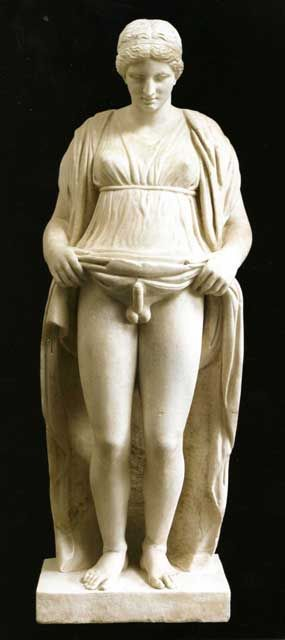
\includegraphics[width=7cm]{shock.jpg}};}%
\end{tikzpicture}
}

At this point let us try the new code and see the small improvements we have done.

\cxset{title font-color=spot!50}
\cxset{subtitle font-color/.store in=\subtitlefontcolor@cx}
\cxset{subtitle font-color=black!35}
\cxset{fashion image=shock.jpg}

% Image needs debugging, something is not capturing it.
\fashion

We have also used a different image and as you can observe with shock, our layout has lost its appeal, will
probably offend some people and the color scheme seems messed up. What we will probably have to do
is add a few more parameters, as well as measure the image’s dimension and implement different rules for
different aspect ratios. Try at this stage and use your own code to modify the layout.

\long\def\storyi{
         In antiquity men and women saw each other as different; 
         accordingly, they developed
        complex taxonomies (philosophical explanations) 
        for understanding anatomical,
        physiological, emotional, and rational differences. \par

Some of these differences seem
profoundly odd to us moderns. Modern discussions about erotic art have often concerned the place of women: to what
extent are they objects of social manipulation, to what extent can they be subjects?
}
\long\gdef\fashion#1{%
\begin{tikzpicture}

\if@debug
  \draw [help lines] (0,0) grid (18,-13);
  \draw[fill=red]  (0,0) circle (1.5pt) ;
  \draw[fill=red]  (0,-3) circle (1.5pt) ;
\else
\fi
% draw debug rectangles
\node[fashion, right, baseline] (x) at (0,1) {\LARGE\color{black!30}{before}\relax};
\draw[fill=red]  (0,1) circle (1.5pt) ;
\node[fashion, right=1sp] at (0,0) {\LARGE\color{black!20} \so\chaptername\relax};

\node[rectangle,draw, color=white, below right, fill=\fashionnumberbg@cx, text=white] at +(12,0) {\scalebox{2}{\HUGE \thechapter}};

% The title of the block
\node[fashion, text width=9cm,below right, yshift=-1pt] at (0,-3) {%
        { \sffamily\raggedleft
        \Huge\bfseries\color{\titlefontcolor@cx}#1\par}
         \bigskip
         \Large% 
         \centering
         \color{\subtitlefontcolor@cx}%
         \raggedleft
        \storyi\par}; 
        \IfFileExists{\fashionimage@cx}%   
           {\node at (12.5,-9) {\includegraphics[width=\imagewidth@cx]{\fashionimage@cx}};}%
           { \node at (12.5,-9) {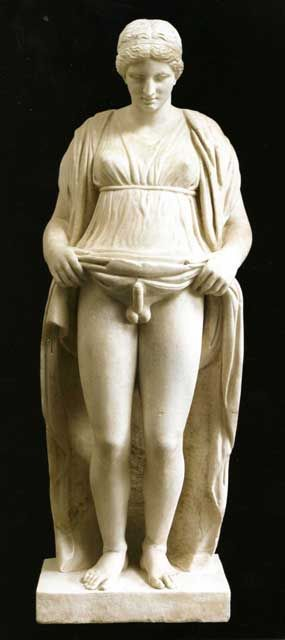
\includegraphics[width=7cm]{shock.jpg}};}%
\end{tikzpicture}
}

\fashion{SEXUALITY IN ANCIENT GREECE}
\makeatother
\bigskip

Using your document as a User Interface is  programming in a hostile environment. As mentioned
earlier, try pen and paper, it is the quickest way to get a layout right. Adding and removing text, in layouts such
as the one we have been developing is an essential part in getting the layout to get the layout aesthetics right.
Of course other people might have different taste than you and what you like would probably be distateful to other persons.
This is a common lamentation of Graphic Designers, who complain about the value systems of their Clients.

\subsection{Hooking onto LaTeX}

I think the layout is now much better and it has evolved to transform itself from a modern and colorful template to a more serious one, perhaps more appropriate for scientific work.

We have now won half the battle, the next battle is to hook into the |\section| or |\chapter| command using |\secdef|. As you might have noticed, the chapter number has not been incremented. We will need to also
add it to the Table of Contents and also get the indentation after the heading to work correctly. We do not want our users to have to worry about this and adding |\noindent|’s all over the place. At this point we will also 
add functions to add the chapter number and title to the Table of Contents. 

\makeatother

\makeatletter\@specialfalse\makeatother
\cxset{
         section font-family=tiresias,
         chapter numbering=arabic,
         chapter title align=none}
\chapter{More on Boxes: Using packages to automate boxing calculations and the drawing of borders.}
\thispagestyle{plain}
\pagestyle{headings}
\large

\section{Testing title values}
\makeatletter
\ExplSyntaxOn
title~display = \int_use:c {chapter_title_display} \\
chapter~title-display= \int_use:c {chapter_title_display} \\
title~display =\meaning\titledisplay@cx\\
chapter~title~text-align = \meaning\chaptertitletextalign@cx\\
%chapter~title~align = \tl_use:c {tl_chapter_title_align}
\meaning\chaptertitletextalign@cx
\makeatother
\ExplSyntaxOff

The boxing of contents is such an important concept in \tex and also in typography that it is worth examining some of the available packages that can be used.

Another elaborate package is Martin Scharrer’s package \pkgname{adjustbox}. The package uses numerous keys
to draw borders, adjust spacing and margins but also for the clipping of images. At the background the package uses and extends the \pkgname{graphicx} key value system.

This package allows to adjust general \latexe material in several ways using a key=value interface.
It got inspired by the interface of \cmd{\includegraphics} from the \pkg{graphicx} package.
 This package also loads the \pkg{trimclip} package which code was once included in this package.


 \subsection{Trimming and Clipping}
 
 Trimming and clipping is achieved by loading the \pkgname{trimclip}. This package forms part of the suit of packages developed by Martin Scharrer and or related to adjusting boxes and their sizes. The package allows for
 verbatim material as well. 
 
 \let\Macro\cmd
 
 The following keys allow content to be trimmed (i.e.\ the official size is made smaller, so the remaining material
 laps over the official boundaries) or clipped (overlapping material is not displayed).
 These keys come in different variants, where the lower-case keys represent the behavior of
 the corresponding \Macro\includegraphics keys. The corresponding macros (\Macro\trimbox, \Macro\clipbox, etc.)
 and environments (\env{trimbox}, \env{clipbox}, etc.) are included in the
 accompanying \pkg{trimclip} package and are explained in its manual.

 
 This key represents the original \option{trim} key of \Macro\includegraphics but accepts its value in different forms.
 Unlike most other keys it always acts on the original content independent in which order it is used with other keys.
 The key trims the given amounts from the lower left (ll) and the upper right (ur) corner of the box. This means that
 the amount \meta{llx} is trimmed from the left side, \meta{lly} from the bottom and \meta{urx} and \meta{ury} from the
 right and top of the box, respectively.
 If only one value is given it will be used for all four sites.
 If only two values are given the first one will be used for the left and right side (llx, urx) and the second for the
 bottom and top side (lly, ury).
 
\begin{texexample}{Example}{clipping}
\adjustbox{Clip=1, min width=8cm, center,}{This is some test}
\medskip

The untrimmed version is shown below
\medskip

\adjustbox{Clip=.1, min width=8cm, center,}{This is some test}%
\end{texexample}
 
\section{tcolorbox} 

\subsection{Breakable Boxes}

 \begin{verbatim}
 \begin{tcolorbox}[enhanced, breakable,
  colback=blue!5!white,colframe=blue!75!black,title=Breakable box,
  watermark color=white, watermark text=\Roman{tcbbreakpart}]
  \lipsum[1-18]
\end{tcolorbox}

	See \ref{test} for details and an example.
 \end{verbatim}
 
 
 

 
\cxset{style87/.style={
 chapter opening=any,
 chapter name=none,
 % positioning and float - inline is 0
 %  float right is 2
 number display=block,
 number float=right,
 number shape=starburst,
 numbering=Words,
 number spaceout=none,
 number font-size=huge,
 number font-weight=bold,
 number font-family=rmfamily,
 number font-shape=normal,
 number before=,
 number display=inline,
 number float=none,
% 
 number border-top-width=0pt,
 number border-right-width=0pt,
 number border-bottom-width=0pt,
 number border-left-width=0pt,
 number border-width=1pt,
%  
 number padding-left=0em,
 number padding-right=0.5em,
 number padding-top=0em,
 number padding-bottom=0pt,
  %number margin-top=, to do
 %number margin-left=0pt,  to create
 %
 number after=\par,
 number dot=,
 number position=rightname,
 number color=sweet,
 number background-color=white,
 %chapter name
 chapter display=block,
 chapter float=left,
 chapter shape=ellipse,
 chapter color=black,
 chapter background-color=sweet,
 chapter font-size= Huge,
 chapter font-weight=bfseries,
 chapter font-family=itshape,
 chapter before=,
 chapter spaceout=none,
 chapter after=,
 chapter margin-left=0cm,
 chapter margin-top=0pt,
 %
 chapter border-width=2pt,
 chapter border-top-width=1pt,
 chapter border-right-width=1pt,
 chapter border-bottom-width=1pt,
 chapter border-left-width=4pt,
% 
 chapter padding-left=20pt,
 chapter padding-right=20pt,
 chapter padding-top=20pt,
 chapter padding-bottom=10pt,
  %chapter title
 title font-family=rmfamily,
 title font-color=spot!80,                    %CHANGED
 title font-weight=bfseries,
 title font-size=huge,
 chapter title align=none,
 title margin-left=1cm,
 title margin-bottom=1.3cm,
 title margin-top=30pt,
 % title borders
 title border-width=0pt,
 title padding=0pt,
 title border-color=black!80,
 title border-top-color=spot!50,
 title border-top-width=2pt,
 title border-left-color=black!80,
 title border-left-width=2pt,
 title border-color=black!80,
 title padding-top=0pt,
 title padding-bottom=0pt,
 title padding-left=0pt,
 title padding-right=0pt,
 title border-right-color=spot!50,
 title border-right-width=2pt,
 title border-bottom-color=spot!50,
 title border-bottom-width=2pt,
 %
 chapter title align=left,
 chapter title text-align=left,
 chapter title width=0.8\textwidth,
 title before=,
 title after=,
 title display=block,
 title beforeskip=12pt,
 title afterskip=12pt,
 author block=false,
 section font-family=rmfamily,
 section font-size=LARGE,
 section font-weight=bfseries,
 section indent=0pt,
  section font-weight=mdseries,
 section align=left,
 subsubsection font-family=tiresias,
 subsubsection font-shape=upshape,
 subsubsection font-weight=mdseries,
 subsubsection align=flushleft,
 epigraph width=\dimexpr(\textwidth-2cm)\relax,
 epigraph align=center,
 epigraph text align=center,
 epigraph rule width=0pt,
 header style=plain}}
 
\cxset{style87}
\renewsection\renewsubsection\renewsubsubsection
\ExplSyntaxOff
\makeatother
\endinput

\makeatletter
\cxset{enumerate numberingi/.is choice,
  enumerate numberingi/.code={\renewcommand\theenumi {\csname#1\endcsname{enumi}}},
  enumerate numberingii/.code={\renewcommand\theenumii {\csname#1\endcsname{enumii}}},
  enumerate numberingiii/.code={\renewcommand\theenumiii {\csname#1\endcsname{enumiii}}},
  enumerate numberingiv/.code={\renewcommand\theenumiv {\csname#1\endcsname{enumiv}}},
  enumerate labeli punctuation/.store in=\enumeratepunctuationi@cx,
  enumerate labeli/.is choice,
  enumerate labeli/brackets/.code={\renewcommand\labelenumi{(\theenumi\enumeratepunctuationi@cx)}},
  enumerate labeli/square brackets/.code={\renewcommand\labelenumi{[\theenumi\enumeratepunctuationi@cx]}},
  enumerate labeli/right bracket/.code={\renewcommand\labelenumi{\theenumi\enumeratepunctuationi@cx)}},
  enumerate label left/.store in=\enumeratelabelleft@cx,
  enumerate label right/.code=\renewcommand\labelenumi{\enumeratelabelleft@cx\theenumi\enumeratepunctuationi@cx#1},
  enumerate leftmargini/.code={\setlength\leftmargini{#1}},
  enumerate leftmarginii/.code={\setlength\leftmarginii{#1}},
  enumerate leftmarginiii/.code={\setlength\leftmarginiii{#1}},
  enumerate leftmarginiv/.code={\setlength\leftmarginiv{#1}},
  listi topsep/.store in=\listitopsep@cx,
  listi partopsep/.store in=\listipartopsep@cx,
  listi itemsep/.store in=\listiitemsep@cx,
  listi parsep/.store in=\listiparsep@cx,
  listii topsep/.store in=\listiitopsep@cx,
  listii partopsep/.store in=\listiipartopsep@cx,
  listii itemsep/.store in=\listiiitemsep@cx,
  listii parsep/.store in=\listiiparsep@cx,
  listiii topsep/.store in=\listiiitopsep@cx,
  listiii partopsep/.store in=\listiiipartopsep@cx,
  listiii itemsep/.store in=\listiiiitemsep@cx,
  listiii parsep/.store in=\listiiiparsep@cx,
}
\cxset{compact1/.style={%
  enumerate numberingi=arabic,
  enumerate numberingii=alph,
  enumerate numberingiii=alph,
  enumerate numberingiv=roman,
  enumerate labeli punctuation=.,
  enumerate label left=,
  enumerate label right=,
  enumerate leftmargini=2.2em,
  enumerate leftmarginii=2.1em,
  enumerate leftmarginiii=1.5em,
  enumerate leftmarginiv=2em,
  listi topsep=8\p@ \@plus2\p@ \@minus\p@,
  listi itemsep=0\p@ \@plus2\p@ \@minus\p@,
  listi parsep=0\p@ \@plus2\p@ \@minus\p@,
  listii topsep=0\p@ \@plus2\p@ \@minus\p@,
  listii itemsep=0\p@ \@plus2\p@ \@minus\p@,
  listii parsep=0\p@ \@plus2\p@ \@minus\p@,
  listiii topsep=0\p@ \@plus2\p@ \@minus\p@,
  listiii itemsep=0\p@ \@plus2\p@ \@minus\p@,
  listiii parsep=0\p@ \@plus2\p@ \@minus\p@,
}}
\cxset{compact2/.style={%
  enumerate numberingi=alph,
  enumerate numberingii=roman,
  enumerate numberingiii=alph,
  enumerate numberingiv=roman,
  enumerate labeli punctuation=,
  enumerate label left=(,
  enumerate label right=),
  enumerate leftmargini=2.2em,
  enumerate leftmarginii=2.1em,
  enumerate leftmarginiii=1.5em,
  enumerate leftmarginiv=2em,
  listi topsep   = 8\p@ \@plus2\p@ \@minus\p@,
  listi itemsep = 0\p@ \@plus2\p@ \@minus\p@,
  listi parsep   = 0\p@ \@plus2\p@ \@minus\p@,
  listii topsep  = 0\p@ \@plus2\p@ \@minus\p@,
  listii itemsep= 0\p@ \@plus2\p@ \@minus\p@,
  listii parsep  = 0\p@ \@plus2\p@ \@minus\p@,
  listiii topsep = 0\p@ \@plus2\p@ \@minus\p@,
  listiii itemsep= 0\p@ \@plus2\p@ \@minus\p@,
  listiii parsep  = 0\p@ \@plus2\p@ \@minus\p@,
}}

\ExplSyntaxOn
\def\setenumerate#1{
\cxset{#1}
\def\@listi{%
           \leftmargin\leftmargini
            \parsep\listiparsep@cx
            \topsep\listitopsep@cx\relax
            \itemsep\listiitemsep@cx}
            
\def\@listii{\leftmargin\leftmarginii
            \parsep\listiiparsep@cx
            \topsep\listiitopsep@cx\relax
            \itemsep\listiiitemsep@cx}
            
\def\@listiii{\leftmargin\leftmarginiii
            \parsep\listiiiparsep@cx
            \topsep\listiiitopsep@cx\relax
            \itemsep\listiiiitemsep@cx}
}


\setenumerate{compact1}

\cxset{section align=left}
\cxset{section font-weight=bold}
\cxset{section font-family=sffamily} 
\cxset{section top rule=false,
          section bottom rule = false,
}
          
          
          
\makeatletter
\cxset{title font-family=\sffamily,
       title font-size=\Huge,
       title font-weight=\bfseries}

\@specialtrue

\cxset{custom=steward}
\cxset{steward,
  chapter toc=true,
  numbering=arabic,
  custom = stewart,
  offsety=0cm,
  image=hine03,
  texti={When Lamport designed the original \LaTeX\ sectioning commands, limitations of computer power forced him to restrict the abstraction of complicated chapter layouts. With current tools available improvements are much easier to program.},
  textii={In this chapter we discuss a method that allows the production of fancy chapter headings and formatting, based on a set of key values. Central  to this process is the separation of content from presentation.
We also discuss the basic formatting tools that are available and how one can modify them to mould new book designs.},
}


\@specialtrue

\cxset{chapter opening=left}
\chapter{Special Designs}
\section{Introduction}


The strength of the package lies in having defined mechanisms to enable easier abstraction of special designs.
We will first outline a simple mechanism for such definitions.

To define any special chapter you need to either redefine a command or create a new one. Let us look at
an example, which simply uses the tikZ package to draw a chapter header at the top of the page. Every time the \cs{chapter} command is called, this command will be indirectly activated at the appropriate point.
What is available for you to use is all the chapter settings information. You can also add additional keys.


The strength of the system lies in defining an adequate number of variables to abstract the design. We also need to decide which are the important parameters. Let us for demonstration purposes just add two new keys.
One for the band color and another for the rounded colour.

Note that any design based on tikZ's  \texttt{remember picture, overlay} requires possibly two and sometimes three runs in order to stabilize.



\section{Naming conventions}

When you set the key custom it redefines the command \cs{customdesign@cx} to hold the name of your special macro.  So the only place where you need to add a definition is one macro. You can name your style anything you want, however I recommend that variants are named in two or more words, the second one simulating a theme. For example you can name your theme \option{stephan} and a sub-theme as  \option{stephan blue}.


\section{Themes and styles}

Once you have a design abstracted and its major components defined as keys, you can think of it as a template. A template then can be extended to different \textit{themes}. For example if we name our template as \textit{stefan}, we can have themes as \textit{stefan blue}, \textit{stefan green} or other similar and appropriate names. This is closer to what is currently used in CMS systems on the web.




\cxset{stefan/.style={%
        title font-color=\color{white},
        band height=5cm,
        fill= teal,
        custom=tikzspecials}}

\cxset{stefan}

\chapter{Special Designs}

\lipsum[1-3]








\chapter{Introduction to TikZ Style Chapters}

The \lstinline{tikZ} package brings a lot of capabilities to the design of fancy style headings, including shading effects and the like. I expect this type of design to grow in the future. Since tikZ is part of the PGF family it is easy to integrate with the package.

\section{Integrating the code}

Code integration, especially with a document that might have different chapter headings presents a challenge. However, if we do touch the chapter command it might make things easier. We provide a key called special that instead of calling the \string\@make... calls a special
routine to handle the tikz commands (as one would expect that all the code will then be here).


First we define a special key.


\begin{teX}
\cxset{custom/.code=\gdef\customdesign@cx{#1}\@specialtrue,
       fill/.store in=\fill@cx}
\cxset{custom=tikzspecial,
       title font-size=\Large,
       title font-color=\color{white}}
\end{teX}

We have assumed that the only value we want to pass is the Chapter title, as the rest can be handled quite easily, by means of key values.

\section{Key management}

When you develop a generic template all the standards keys are available to you. For example the chapter opening commands. However, if you positioning using fixed parameters, the anywhere key cannot work properly, by adding a yshift into the definition of the special and adjusting you can achieve it.

\clearpage



\cxset{stefan,
       chapter opening=anywhere,
       fill= purple,
       band height=2cm,
       section color= purple}

\renewsection

\chapter{A test}

\section{Conclusions}

In this chapter we have seen how to design and code special templates for special openings. In most cases you will use TikZ to produce them, so familiarity with the graphics program is essential. In general I advice that before you embark on a special design to select the method you will used based on the following:

\begin{enumerate}
\item If the template requires positioning of pictures and text at exact positions, you can use the 
        picture environment and the built-in commands provided in this package.
\item If it requires any special graphics, coloured blocks and the like, use the TikZ package or pstricks.
\item If you only manipulating textual information you don't need a special use the key value interface provided by the package (see for example the verso style).
\end{enumerate}


\clearpage

\newgeometry{top=1cm,bottom=1cm,left=0cm, right=0cm} 


\pagestyle{empty}

\@specialfalse
\cxset{
 custom= genetics,
 name={CHAPTER CONCEPT},
 numbering=none,
 number font-size=,
 number font-family=,
 number font-weight=,
 number color=white,
 numbering=arabic,
 chapter opening=right,
 chapter color={black},
 chapter font-family=\sffamily,
 chapter font-size=\Large,
 chapter font-weight=\bfseries,
 title font-family=\sffamily,
 title font-color=teal,
 rule off,
 image=genetics-dogs,
 image caption={Labrador retriever\\
         puppies expressing\\
         brown (chocolate),\\
         golden (yellow),\\
         and black\\
         coat colors,\\
         traits controlled\\
         by two gene pairs.},
 textiii={\begin{itemize}
\large
\item This is some text describing the main chapter concepts. Many
      modern textbooks have chapter openings, with complicated
      layouts, such as this one.
\item Each layout is probably unique, but some designs
      might be possible to be abstracted.
\item Keys are defined for the special textboxes in a anti-clockwise pattern.
      The image caption is set using image caption, the chapter concepts list
      is defined using the key textiii.
\item The chapter number is available via the normal chapter number keys.
\item This layout has been developed using normal \tex macros and does not
      utilize absolute positioning via tikz or similar. This way the layout
      is more flexible. It can certainly be improved using LaTeX3 techniques.
  \end{itemize}}
}


\newpage
\@specialtrue
\chapter[Special Design]{Extensions\\ of Mendelian\\ Genetics}


\cxset{
 custom=genetics,
 name={CHAPTER CONCEPT},
 numbering=none,
 number font-size=,
 number font-family=,
 number font-weight=,
 number color=white,
 numbering=arabic,
 chapter opening=right,
 chapter color={black},
 chapter font-family=\sffamily,
 chapter font-size=\Large,
 chapter font-weight=\bfseries,
 title font-family=\sffamily,
 title font-color=teal,
 rule off,
 image= chromosome,
 image caption={Labrador retriever\\
         puppies expressing\\
         brown (chocolate),\\
         golden (yellow),\\
         and black\\
         coat colors,\\
         traits controlled\\
         by two gene pairs.},
 textiii={\begin{itemize}
\large
\item While alleles are transmitted from parent to   offspring
according to Mendelian principles, they often do not
display the clear-cut dominant/recessive relationship
observed by Mendel.
\item In many cases, in a departure from Mendelian genetics,
two or more genes are known to influence the phenotype
of a single characteristic.
\item Still another exception to Mendelian inheritance occurs
when genes are located on the X chromosome, because one
of the sexes receives only one copy of that chromosome,
eliminating the possibility of heterozygosity.
\item Phenotypes are often the combined result of genetics and
the environment within which genes are expressed.
\item The result of the various exceptions to Mendelian principles
is the occurrence of phenotypic ratios that differ from those
produced by standard monohybrid, dihybrid, and trihybrid
crosses.
  \end{itemize}
}}

\newpage

\chapter[Jia Lu's paintings]{The Human\\Chromosome}



\newpage

\cxset{custom = genetics,
 image = swords,
 image caption={Liu's paintings\\
         reflect traditional\\
         aesthetics of,\\
         her teacher\\
         Fang Zeng.\\
         Her work\\
         reflects strength\\
         and wisdom.},
 textiii={\begin{itemize}
\large
\item While alleles are transmitted from parent to   offspring
according to Mendelian principles, they often do not
display the clear-cut dominant/recessive relationship
observed by Mendel.
\item In many cases, in a departure from Mendelian genetics,
two or more genes are known to influence the phenotype
of a single characteristic.
\item \lorem
  \end{itemize}
}}

\chapter[swords]{Jia Lu's\\Sensual\\Paintings}

\restoregeometry

\section{Jia Lu}

Jia Lu is an oil painter working in America, known for blending Asian and European imagery in her paintings, predominantly of women. Jia Lu's works include Chinese ink paintings, oil paintings, watercolors, drawings, sculpture and prints. Her early work strongly reflected the traditional aesthetics of her teacher Fan Zeng, but by the time she exhibited in Canada, she was critiquing new social developments, consumerism and power relations in China through a series of mixed-media self-portraits. Her mature work in oils demonstrates an interest in Buddhism and a purely feminine aesthetic and can be seen as a response to the masculine, sensual approach to the female nude. However, she has also painted male figures. In numerous interviews she has emphasized the importance of beauty in her work, which she describes as "strength and wisdom".

\makeatletter
\@specialfalse











%% DESIGNING HEADERS AND FOOTERS  **************************


\cxset{chapter toc=true, custom = stewart,}
\cxset{steward,
  offsety=0.5cm,
  image=hine05,
  texti={A ball falls faster and faster as time
        passes. Galileo discovered that the
        distance fallen is proportional to the
        square of the time it has been falling.
        Calculus then enables us to calculate the
        speed of the ball at any time.}, % do not forget the commas.
  textii={The fundamental objects that we deal with in calculus are functions. We stress that a function can be
represented in different ways: by an equation, in a table, by a graph, or in words. We look at the main
types of functions that occur in calculus and describe the process of using these functions as mathematical
models of real-world phenomena.
In \textit{A Preview of Calculus} (page 1) we saw how the idea of a limit underlies the various branches of
calculus. It is therefore appropriate to begin our study of calculus by investigating limits of functions and
their properties}
}

\cxset{chapter opening=left,
          header style=empty}

\chapter{Setting headers and footers}

\section{Setting Headers and Footers}
One of the first tasks of any \LaTeXe\ class is to redefine the headers and footers. The format of the running headers or footers in \LaTeX\ terminology is called the \textit{page style}. Each different format is given names like \textit{empty} or \textit{plain} to make it easier to select and remember.


\section{Traditional LaTeX page style commands}
The LaTeX kernel\footnote{In File J \file{ltpage.dtx}, page 311.} defines two commands for selecting the running heads:

\begin{lstlisting}
\pagestyle{<style>} : sets the page style of the current and succeeding pages to style
\thispagestyle{<style>} : sets the page style of the current page only to style.
\end{lstlisting}

\section{Traditional LaTeX page style definition}
To define a page style \textit{style}, you must define the \lstinline{\ps@style} to set the page parameters.

\subsection{How a page style makes running heads and feet}
The \lstinline{\ps@}. . . command defines the macros \lstinline{\@oddhead}, \lstinline{\@oddfoot}, \lstinline{\@evenhead},
and \lstinline{\@evenfoot} to define the running heads and feet. (See output routine.) As some headings contain information such as the chapter name or section number these
headings are based on the sectioning commands, which define them. The page style defines the commands




\verb!\chaptermark,\sectionmark!, etc., where

\verb+\chaptermark{<text>}+ is called by \verb+\chapter+ to set a mark. The  ...mark commands and the ...head
macros are defined with the help of the following macros.
%(All the \ ...mark commands should be initialized to no-ops.)



\subsection{marking conventions}

LaTeX produces two kinds of marks a `left' and a `right' mark using the following commands.

markboth

markright



\section{The low level page style interface}
The basic mechanics of defining page styles is provided in the \LaTeXe\ kernel and it  involves defining or redefining four macros:

\begin{marglist}
\item [\cs{oddhead}] For two-sided printing, it generates the header for the odd-numbered
pages; otherwise, it generates the header for all pages.

\item [\cs{oddfoot}] For two-sided printing, it generates the footer for the odd-numbered pages; otherwise, it generates the footer for all pages.

\item [\cs{evenhead}] For two-sided printing, it generates the header of the even-numbered
pages; it is ignored in one-sided printing.

\item [\cs{evenfoot}] For two-sided printing, it generates the footer of the even-numbered
pages; it is ignored in one-sided printing.

\end{marglist}
A named page style, involves the redefinition of these commands stored in a macro \cs{ps@<style>}.
The \cs{pagestyle}\marg{plain} is defined as:



%\begin{tcolorbox}
%\begin{lstlisting}
%\newcommand\ps@plain{%
%  \renewcommand\@oddhead{}%
%  \let\@evenhead\@oddhead
%  \renewcommand\@evenfoot{%
%  {\hfil\normalfont\textrm{\thepage}\hfil}}%
%  \let\@oddfoot\@evenfoot
%}
%\end{lstlisting}
%\end{tcolorbox}

Since the \textit{plain} style treats both the odd and even pages the same way, the \cs{@evenfoot} and \cs{@evenhead} are let to the \cs{@oddhead} and \cs{@oddfoot} commands. The style only prints a page number at the center of the footer.


\subsection{A longer example}

\index{watermark}\index{water mark!sample page style}
\thispagestyle{samplepage}
Consider the case, where we need to print on a page the words \textsc{sample page}, as you might have noticed in some places of this document and at the margin of this page. Sometimes this type of mark is called a \textit{watermark.}

We will call this type of page style \textit{samplepage} and we will activate it on a particular page by typing \cs{thispagestyle}\marg{samplepage}.




%\begin{tcolorbox}
%\begin{lstlisting}
%%% Some special styles
%\IfFileExists{rotating.sty}{\RequirePackage{rotating}}{}
%
%\def\even@samplepage{%
% \begin{picture}(0,0)
%   \put(\Xeven,\Yeven){\turnbox{90}{\Huge \textcolor{\watermark@textcolor}{\watermark@text}}}
%\end{picture}
%}
%
%\def\odd@samplepage{%
% \begin{picture}(0,0)
%   \put(\Xodd,\Yodd){\turnbox{90}{\Huge \textcolor{\watermark@textcolor}{\watermark@text}}}
% \end{picture}
%}
%
%\def\watermarktext#1{\gdef\watermark@text{\fontfamily{phv}\selectfont#1}}
%\def\watermarktextcolor#1{\gdef\watermark@textcolor{#1}}
%\watermarktext{SAMPLE PAGE}
%\watermarktextcolor{purple}
%
%\def\ps@samplepage{\let\@mkboth\@gobbletwo
% \let\@oddhead\odd@samplepage\def\@oddfoot{\reset@font\hfil\thepage}
% \let\@evenhead\even@samplepage\def\@evenfoot{\reset@font\thepage\hfil}}
%
%\def\Xodd{500}
%\def\Xeven{-70}\def\Yeven{-810}
%\def\Yeven{-\expandafter\strip@pt\textheight}
%\let\Yodd\Yeven
%\end{lstlisting}
%\end{tcolorbox}

If you study the code in the example, you will notice that we are using \LaTeXe's \env{picture} environment to
place the text exactly where we need it.




\subsection{The key value interface}

The key value interface provides a number of mechanisms to tap into the page styles, enabling consistency in the user interface.

\medskip

\keyval{header style}{\marg{text}}{Triggers a page style for one page only.} The following values can be used.

\begin{marglist}
\item [empty] Standard class empty headers.
\item [plain] Standard class plain headers.
\item [headings] Standard class headings.
\item [fancy] If you use the fancyhdr package any fancy header style.
\item [sample page] Prints sample at the edge of the paper.
\item [preprint] Prints preprint at the edge of the paper.
\item [watermark] Prints a watermark at predefined places.
\end{marglist}

\keyval{watermark}{\marg{true|false}}{Prints a water on all pages, defaults to false.}
\keyval{watermark text}{\marg{text}}{The watermark text.}
\keyval{watermark text left}{\marg{text}}{The watermark text on left pages.}
\keyval{watermark text right}{\marg{text}}{The watermark text on right pages.}
\keyval{watermark angle}{\marg{number}}{The rotation angle of the water mark}




%\cxset{ watermark text/.store in=\watermark@text,
%           watermark text color/.store in=\watermark@textcolor,
%           watermark font-size/.store in=\watermarkfontsize@cx,
%           watermark odd x/.store in=\watermarkoddx@cx,
%           watermark even x/.store in=\watermarkevenx@cx,
%           watermark even y/.store in=\watermarkeveny@cx}
%
%\cxset{watermark text= PRE-PRINT,
%          watermark text color=theblue,
%          watermark font-size=\huge,
%          watermark odd x=470,
%          watermark even y=700,
%          watermark even x=60}
%
%\def\Xodd{\watermarkoddx@cx}
%\def\Xeven{-\watermarkevenx@cx}
%\def\Yeven{-\watermarkeveny@cx}
%%\def\Yeven{-\expandafter\strip@pt\textheight}
%\let\Yodd\Yeven
%
%\def\even@samplepage{%
% \begin{picture}(0,0)
%   \put(\Xeven,\Yeven){\turnbox{60}{\watermarkfontsize@cx \textcolor{\watermark@textcolor}{\watermark@text}}}
%\end{picture}
%}
%
%\def\odd@samplepage{%
% \begin{picture}(0,0)
%   \put(\Xodd,\Yodd){\turnbox{90}{\watermarkfontsize@cx\textcolor{\watermark@textcolor}{\watermark@text}}}
% \end{picture}
%}






\subsection{Example usage}

We will now show an example using the key value interface to illustrate the concepts and the usage. We will change the watermark text, color and font on this page. If you notice at the right bottom of the page the word \textsc{PRE-PRINTED} has been printed in blue.

\begin{tcolorbox}
\begin{lstlisting}
\cxset{
     watermark text= PRE-PRINT,
     watermark text color=theblue,
     watermark font-size=\huge
}
\end{lstlisting}
\end{tcolorbox}

\thispagestyle{samplepage}

\clearpage

\section{Adding marks}

Most books will have headers that include marks such as the chapter name and number and or other combinations together with section numbers.

The standard book class include two styles one called \textit{headings} and another called \textit{myheadings} that style such headers.




\subsection{Key value interface}
\makeatletter
\cxset{
   chaptermark name color/.store in=\chaptermarknamecolor@cx,
   sectionmark name color/.store in=\sectionmarkcolor@cx,
   sectionmark title font/.store in=\sectionmarktitlefont@cx,
   section title color/.store in=\sectiontitlecolor@cx,
}

\makeatother

\cxset{chaptermark name color=thered,
          sectionmark name color=thered}








\begin{tcolorbox}
\begin{lstlisting}
%% STYLE 57 QUANTUM FRONTIER
\cxset{headings style57/.style={
          headings titlestyle,
% Chaptermarks
          chaptermark name={\bfseries EVOLUTION OF THE INSECTS},
% Leftmarks
          leftmark before=\thepage\quad, %even pages
          leftmark after=\hfill\hfill,
% Right marks influenced by chapter name?
          rightmark before=\hfill\hfill, %odd pages
          rightmark after=\thepage,
% Section marks
          sectionmark name custom=\chaptertitle@cx,
          sectionmark after title=\quad,
%  rules we remove or inherit
          header top rule=false,
          header bottom rule=false,
          header offset even=0pt,
          header offset odd=0pt,
          }}
\end{lstlisting}
\end{tcolorbox}


%\if@twoside
%  \def\ps@headings{%
%      \let\@oddfoot\@empty
%      \def\@oddfoot{\rule{\textwidth}{0.4pt}}
%      \let\@evenfoot\@empty
%      \def\@evenhead{\parbox{\textwidth}{%
%                                   \leavevmode
%                                   \if@headertoprule\rule{\textwidth}{0.4pt}%
%                                       \vskip2pt plus1pt minus1pt\fi
%%typesetter
%                                     \hskip\headeroffseteven@cx\hbox to \textwidth{%
%                                           \leftmarkbefore@cx
%                                           \leftmark
%                                           \leftmarkafter@cx
%                                     }%
%                                     \if@headerbottomrule\vskip-7pt plus1pt minus1pt
%                                    \rule{\textwidth}{0.4pt}\fi%
%          }% end parbox
%       }%
%%% Defines the odd head
%      \def\@oddhead{
%         \parbox{\textwidth}{%
%                                   \leavevmode
%                                   \if@headertoprule\rule{\textwidth}{0.4pt}%
%                                       \vskip2pt plus1pt minus1pt\fi
%%typesetter
%                                     \hskip\headeroffsetodd@cx\hbox to \textwidth{%
%                                           \rightmarkbefore@cx
%                                           \rightmark
%                                           \rightmarkafter@cx
%                                     }%
%                                     \if@headerbottomrule\vskip-7pt plus1pt minus1pt
%                                    \rule{\textwidth}{0.4pt}\fi%
%          }% end parbox
%      }%
%      \let\@mkboth\markboth
% % chaptermark called by chapter and also by table of contents etc. This is essentially a
%%  leftmark
%\def\chaptermark##1{%
%     \gdef\chaptertitle@cx{##1}%
%      \markboth {%
%       \ifnum \c@secnumdepth >\m@ne
%          \if@mainmatter%
%              \color{\chaptermarknamecolor@cx}%
%              \MakeUppercase{\chaptermarkname@cx\ }%
%              \chaptermarknumber%
%              \chaptermarkafternumber@cx%
%          \fi
%        \fi
%        \color{\chaptermarktitlecolor@cx}%
%       % \hfill%
%        \MakeUppercase{\chaptermarktitlebefore@cx{##1}}}{}%
%}%end chaptermark
%% section
%  \def\sectionmark##1{%
%      \markright {%
%        \ifnum \c@secnumdepth >\z@
%           {\bfseries\textcolor{\sectionmarkcolor@cx}{\sectionmarkname@cx\sectionmarknumber@cx\sectionmarkafternumber@cx}%
%        } %
%  \fi
%         \color{\sectionmarktitlecolor@cx}\MakeUppercase{\normalfont\sffamily \sectionmarkbeforetitle@cx{##1}\sectionmarkaftertitle@cx}}}}%
%\else
%  \def\ps@headings{%
%    \let\@oddfoot\@empty
%    \def\@oddhead{{\slshape\rightmark}\hfil\thepage}%
%    \let\@mkboth\markboth
%    \def\chaptermark##1{%
%      \markright {%
%        \ifnum \c@secnumdepth >\m@ne
%          \if@mainmatter
%            \@chapapp\ \thechapter... \ %
%          \fi
%        \fi
%        ##1}}}
%\fi
%\def\ps@myheadings{%
%    \let\@oddfoot\@empty\let\@evenfoot\@empty
%    \def\@evenhead{\thepage\hfil\slshape\leftmark}%
%    \def\@oddhead{{\slshape\rightmark}\hfil\thepage}%
%    \let\@mkboth\@gobbletwo
%    \let\chaptermark\@gobble
%    \let\sectionmark\@gobble
% }

Note that the \cs{markboth} command takes two arguments the left mark and the right mark. It works reasonably well.



%\cxset{headings boxedpagenumber}
%\cxset{headings style58}
%\pagestyle{headings}

\clearpage
\cxset{header style=empty}
\chapter{SAMPLE HEADERS AND FOOTERS}

%\section{Using the fancyvrb package}
%
%Most LaTeX users, when redesigning running headers or footers will use the fancyvrb package. This well established package by Piet van
%Oostrum, allows easy customization of page headers and footers. The default page style provided by fancyhdr is named fancy. It should be activated via
%\lstinline{\pagestyle} after any changes to textwidth are made, as fancyhdr initializes
%the header and footer widths using the current value of this length.
%The look and feel of the fancy page style is determined by six declarations
%Balle 1I1[l'rtace that define the material that will appear on the left, center, and right of the header
%and footer areas. For example, lhead specifies what should show up on the left
%in the header area, while cfoot defines what will appear in the center of the
%footer area. The results of all six declarations are shown in the next example.
%
%\section{Header and footer options of the chaptersx package}
%
%To keep a consistent and familiar interface, the package uses the
%fancyhdr package which it loads by default and defines option keys that are similar to the macros provided by fancyhdr, as well as some additional typesetting keys.
%
%It is also possible to group these in styles, which we have done for the following:
%
%We have endeavoured o include as many keys possible in order to provide a consistent and comprehensive style.
%
%\section{Example header style}


\section{Description of the header engine}

The header engine works by defining three vertical regions to contain a top and bottom rule or other material and a middle layer that contains the text and or graphical material. In its simpler form is an assembly of boxes as shown in figure~\ref{fig:headerengine} .
\medskip

\noindent\vbox{

\framebox[80pt]{toprule}

\fbox{\fbox{offset}$\rightarrow$\fbox{\fbox{name} \fbox{number} \fbox{title} \fbox{page number}}}

\framebox[80pt]{bottomrule}

\captionof{figure}{Typical assembly of boxes for a header}
\label{fig:headerengine}
}

Of course the order of display of the various components can vary, for example in figure~\ref{fig:headerengine01}, we have the page number to the left.

\noindent\fbox{\vbox{%
oddhead\par
\framebox[80pt]{toprule}

\fbox{\fbox{offset}$\rightarrow$\fbox{\fbox{page number}\fbox{name} \fbox{number} \fbox{title} }}

\framebox[80pt]{bottomrule}

\captionof{figure}{Typical assembly of boxes for a header}
\label{fig:headerengine01}
}}

The LaTeX engine as previously described allows for an oddhead and evenhead macros to hold the typesetting information. The typesetting information is obtained asynchrnously,

The chaptermark assembles and stores

\fbox{\fbox{chapter name}$\rightarrow$\fbox{chapter number}$\rightarrow$\fbox{chapter title}}

whereas the sectionamark similarly stores information on section numbering:

\begin{figure}[h]
\fbox{\fbox{section name}\fbox{section number}\fbox{section title}}
\end{figure}

This information of the mark macros is then activated by the leftmark and rightmark commands and when the typesetter calls the oddhead and evenhead the page number is added. So to have a complete definition
we need to define both the marks as well as the oddhead and evenhead macros. Similarly the pagenumber's position can vary in different designs.

The approach we took is to firstly extend the informtion held in each box, for example, the chaptername
looks more like:

\begin{figure}[h]
   \fbox{chaptername before}$\rightarrow$\fbox{chaptername}$\rightarrow$\fbox{chapternameafter}
\end{figure}

Similarly the header elements, \textit{name, number, title} and \textit{pagenumer}  hold information to add material before and after the element. This adds complexity, but generalizes and abstracts the problem nicely.

Now back to leftmarks and rightmarks. The leftmark or rightmark is called by the oddside or evenside macros. We suitably add macros for before and after.

\fbox{before mark}$\rightarrow$\fbox{leftmark or rightmark}$\rightarrow$\fbox{after mark}

\subsection{Discussion}

One would argue that this is a convoluted way of describing the header and footers. However, to have a truly flexible system (with no macro writing for designers and authors) one has to resort to such a long way. It is in many respects simlar to CSS. A looks description language needs as many variables and as much flexibility as possible. The one up on CSS is that the template can be saved and themes developed and invoked very simply.

\subsection{Example settings}
\index{Styles!style56}
\index{Header and footers!example}
To define a style based on the \textit{headings} pagestyle. We will base the style definition on figure~\ref{globalstrategy}. The interesting part of this design is that the chapter numbers are not shown shown in the introduction (which is treated as front matter material). The rest of the chapters are numbered, although the header information and styling remains the same.

\begin{figure}[hp]
\centering
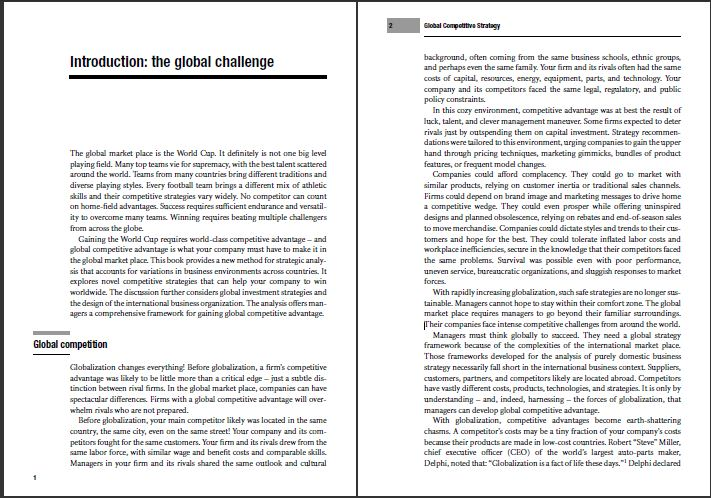
\includegraphics[width=0.8\textwidth]{chapter56}\vspace{0.5\baselineskip}
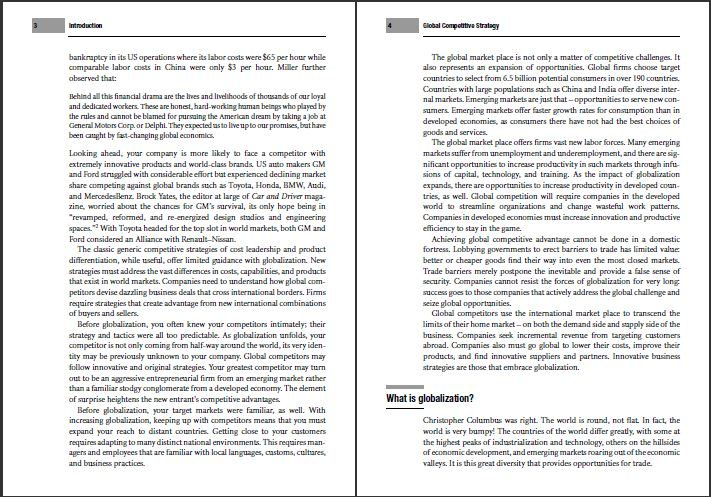
\includegraphics[width=0.8\textwidth]{chapter56a}
\caption{Example pages from \textit{Global Competitive Strategy}, by Daniel F. Spulber,} Cambridge University Press, 2007.
\label{globalstrategy}
\end{figure}

The interesting part of this design is that the headers as well as the chapter openings vary. On the even page the words ``Golbal Competitive Strategy'' are printed, which is the book title\footnote{Although it is an attractive design, it does not mean that this way of header information is a good way of structuring information.}.

Note that since LaTeX only provides two mark we need to arrange our own typesetting rules, we will abuse the macros to achieve it.

\begin{tcolorbox}
\begin{lstlisting}
\cxset{headings style56/.style={
          pagestyle=headings,
          header style=headings,
% Chaptermarks
          chaptermark name color=black,
          chaptermark after number=,
          chaptermark name=SHORT BOOK TITLE,
          chaptermark numbering=none,
          chaptermark title color=black!80,
          chaptermark title before=\@gobble,
% Leftmarks
          leftmark before=\colorbox{thegray!50}{\thepage\quad}\quad, %even pages
          leftmark after=\hfill\hfill,
% Right marks influenced by chapter name?
          rightmark before=\colorbox{thegray!50}{\thepage\quad}\quad, %odd pages
          rightmark after=\hfill\hfill,
% Section marks
          sectionmark name custom=\chaptertitle@cx,
          sectionmark number=none,
          sectionmark name color=black,
          sectionmark title color=black!80,
          sectionmark before title=\@gobble, % we do not need the section title
          sectionmark after title=\hfill\hfill,
          sectionmark after number=,
%  rules we remove or inherit
%       header top rule=false,
          header bottom rule=true,
          header offset even=-1.3cm,
          header offset odd=-1.3cm,
          }}
\end{lstlisting}
\end{tcolorbox}

The approach we need to take here is to first define the even pages, which contain the book short title. Instead of printing the \cs{chaptername}, we give the value of the title to the \textbf{chaptermark} key.

\begin{tcolorbox}
   chaptermark name = SHORT BOOK TITLE,
\end{tcolorbox}

Offsetting the page numbers is done by using the \textbf{header offset} key. As both the left as well as the right pages have the page on the left we offset both of them by the same amount.

\begin{tcolorbox}
\begin{lstlisting}
    chaptermark name = SHORT BOOK TITLE,
    header offset even = -1.3cm,
    header offset odd  = -1.3cm,
\end{lstlisting}
\end{tcolorbox}

\subsection{Inheriting and transforming styles}
One of the advantages of this method, is that we can inherit styles and transform styles easily. Consider style57, which is shown in figure. This is a simple design and follows trends to include the book title in the header. This is a very similar design to header \textit{style57}.

\begin{tcolorbox}
\begin{lstlisting}
%% STYLE 57 QUANTUM FRONTIER
\cxset{headings style57/.style={
          headings style56,
% Chaptermarks
          chaptermark name={\bfseries The Quantum Frontier},
% Leftmarks
          leftmark before=\thepage\quad, %even pages
          leftmark after=\hfill\hfill,
% Right marks influenced by chapter name?
          rightmark before=\hfill\hfill, %odd pages
          rightmark after=\thepage,
% Section marks
          sectionmark name custom=\chaptertitle@cx,
          sectionmark after title=\quad,
%  rules we remove or inherit
          header top rule=false,
          header bottom rule=false,
          header offset even=0pt,
          header offset odd=0pt,
          }}
\end{lstlisting}
\end{tcolorbox}

A crude form of object inheritance is possible by including a style at the top of the key definitions in this case \texttt{headings style56}, we then only need to redefine the values for the changes. We also set zero all offsets and adjust the widths.

The success of the method is defining an appropriate set of general commands and building a community chest of styles.

This concludes the long excursion into headers and footers. This class and method of styling is brand new and is bound to evolve, as it is being used. Feedback is most welcomed as well as bug reports.
\begin{figure}[tp]
\centering
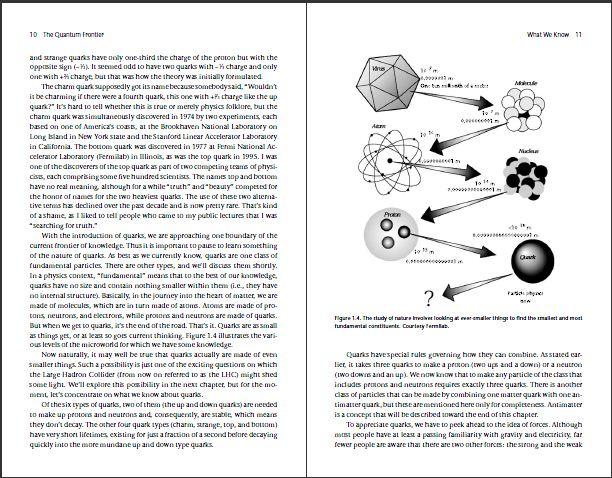
\includegraphics[width=0.8\textwidth]{chapter57a}\vspace{0.5\baselineskip}
\caption{Example pages from \textit{The quantum frontier: the large hadron collider}, by Don Lincoln, The Johns Hopkins University Press, 2009.  It uses the book short-title at even pages and the chapter title at the odd pages.}
\end{figure}

\section{Another inheritance example}

This example is from the book \textit{Evolution of the Insects} by David Grimaldi and Michael S. Engel and published by the Cambridge University Press in 2005. It is a beautifully typeset book and a fine piece of scientific work. The only difference in the headers of the previous examples is the setting of the page number and header text. This one as well as many other books uses the title of the book and the chapter name.

\begin{tcolorbox}
\begin{lstlisting}
%% EVOLUTION OF THE INSECTS
\cxset{headings style58/.style={
          headings style57,
          chaptermark name={\bfseries EVOLUTION OF THE INSECTS},
          leftmark before=\thepage\quad\hfill\hfill, %even pages
          leftmark after=,
          rightmark before=, %odd pages
          rightmark after=\hfill\hfill\thepage,
 }}
\end{lstlisting}
\end{tcolorbox}

Since most of the information was captured in \textit{style57} we inherit the values and only supply the ones  that are changing. This involves changing six settings, illustrating the strength of the procedure adopted. Just a word of caution I found it difficult to follow some of the terminology, if you confused by what a leftmark and right mark are think of them as holding all the header information except the page number.



\begin{figure}
\centering
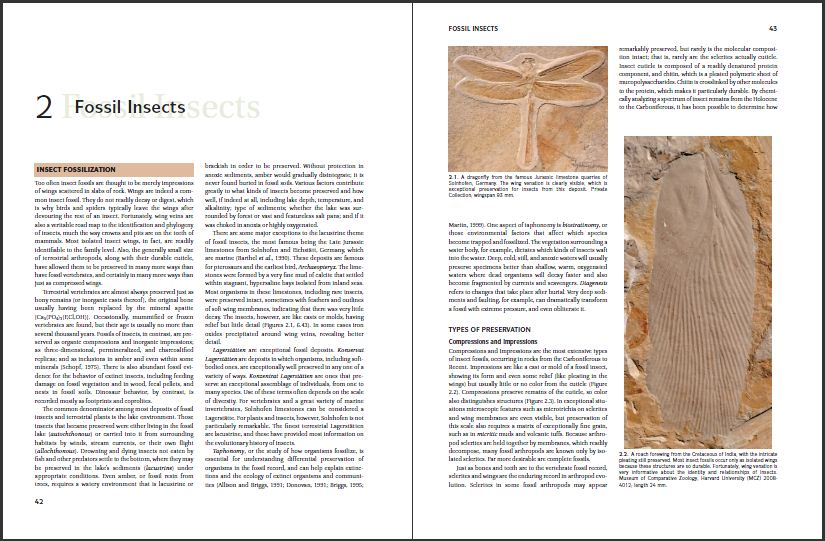
\includegraphics[width=0.8\textwidth]{chapter58}\vspace{0.5\baselineskip}
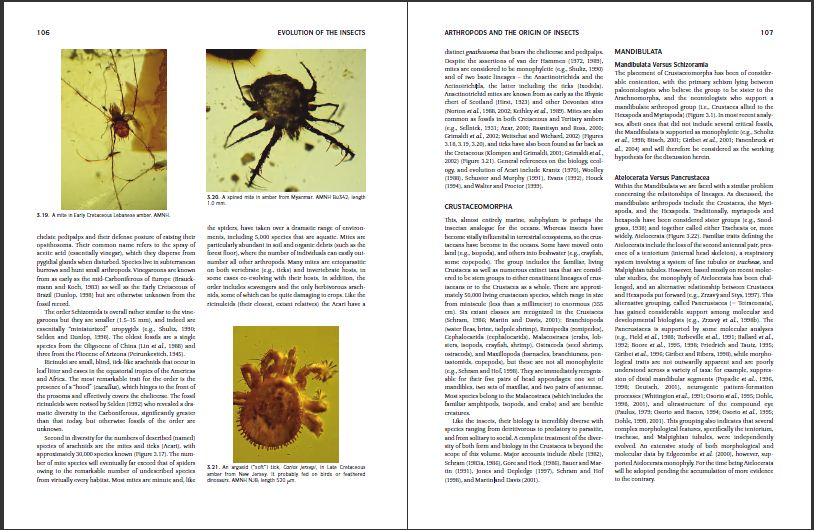
\includegraphics[width=0.8\textwidth]{chapter58a}
\caption{This example is from the book \textit{Evolution of the Insects}, David Grimaldi and Michael S. Engel,  Cambridge University Press, 2005. It is a beautifully typeset book and a fine piece of scientific work. The only difference in the headers of the previous examples is the setting of the page number and header text. This one as well as many other books use the title of the book and the chapter name in headers. The footers are empty with th exception of the chapter page}
\end{figure}


\begin{figure}
\centering
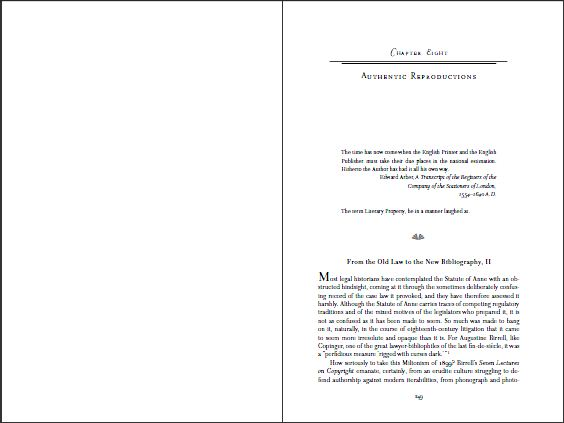
\includegraphics[width=0.8\textwidth]{chapter55}\vspace{0.5\baselineskip}
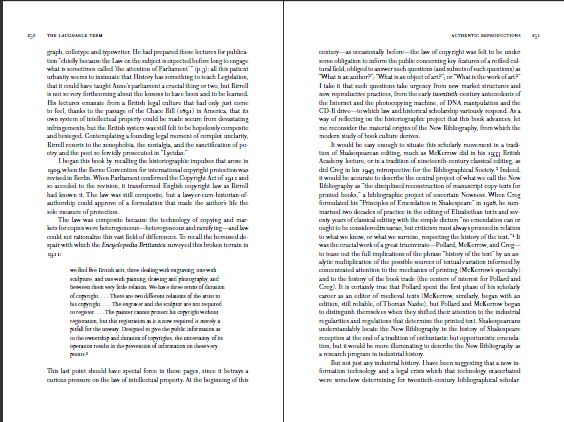
\includegraphics[width=0.8\textwidth]{chapter55a}
\caption{Example pages from \textit{The Author's Due, Printing and the Prehistory of Copyright}, by Joseph Lowewenstein, The University of Chicago Press, 2002.  It uses the part title on the even page and the chapter title on the odd page. The page number is set in the margin. The footers are clear.}
\end{figure}


\clearpage
\thispagestyle{empty}


%%%%%%%%%% NEW GEOMETRY
\newgeometry{top=1cm,bottom=2cm,left=2cm}

%% GENETICS
\@specialfalse
\cxset{
 custom=,
 name={CHAPTER CONCEPT},
 numbering=none,
 number font-size=,
 number font-family=,
 number font-weight=,
 number color=white,
 numbering=arabic,
 chapter opening=right,
 chapter color={black},
 chapter font-family=\sffamily,
 chapter font-size=\large,
 chapter font-weight=\bfseries,
 title font-family=\sffamily,
 title font-color=teal,
 rule off,
}

\begin{specialchapter}[
     image=genetics-dogs,
     image caption={Labrador retriever\\
         puppies expressing\\
         brown (chocolate),\\
         golden (yellow),\\
         and black\\
         coat colors,\\
         traits controlled\\
         by two gene pairs.}]%
{Extensions\\ of Mendelian\\ Genetics}
\begin{itemize}
\item While alleles are transmitted from parent to   offspring
according to Mendelian principles, they often do not
display the clear-cut dominant/recessive relationship
observed by Mendel.
\item In many cases, in a departure from Mendelian genetics,
two or more genes are known to influence the phenotype
of a single characteristic.
\item Still another exception to Mendelian inheritance occurs
when genes are located on the X chromosome, because one
of the sexes receives only one copy of that chromosome,
eliminating the possibility of heterozygosity.
\item Phenotypes are often the combined result of genetics and
the environment within which genes are expressed.
\item The result of the various exceptions to Mendelian principles
is the occurrence of phenotypic ratios that differ from those
produced by standard monohybrid, dihybrid, and trihybrid
crosses.
  \end{itemize}
\end{specialchapter}


%%%%%%%%%% NEW GEOMETRY
\newgeometry{top=2cm,bottom=2cm,left=2cm}
\clearpage

\begin{tcolorbox}
\begin{lstlisting}
%% Special Chapter command
\newcommand\specialchapter@cx[2][]{%
\refstepcounter{chapter}
\cxset{image/.store in=\image@cx,
       image caption/.store in=\caption@cx}
\cxset{#1}
\vbox to 0pt{\color{blue}\rule{\paperwidth}{0.4pt}\par\vskip-1.4pt
\rule{0.4pt}{\textheight}\rule{4cm}{0.4pt}}

\vbox to 0pt{\parbox[b]{4.7cm}{%
\raggedright

\leftskip1.5cm
\caption@cx\par
 \expandafter\rule{\rulewidth@cx}{5.8cm}
}\parbox[b]{0.5cm}{
\includegraphics[width=0.5cm,height=9.15cm]{./chapters/shadow}}\includegraphics{./chapters/\image@cx}\par}

\vspace{8.2cm}
\hspace*{-3.51cm}\hbox to 0pt{\hspace*{1.01cm}
\includegraphics[width=7.7cm,height=3.8cm]{./chapters/genetics-band}
\hspace*{-2.7cm}\sffamily\color{\numbercolor@cx}\HHUGE \raise30pt\hbox{\thechapter}%
\hspace{1.5cm}\raise0.5pt\hbox{
\includegraphics{./chapters/chapterconcept}
\includegraphics{./chapters/shadow2}}
}

%% Title name
\parbox[b]{0.45\textwidth}{%
  \titlefontsize@cx
  \titlefontweight@cx
  \titlefontfamily@cx
  \leftskip0.5em \color{\titlefontcolor@cx}
  #2
}
%% Concepts
}

\newenvironment{specialchapter}[2][]{%
  \if@openright\cleardoublepage\else\clearpage\fi
    \thispagestyle{plain}%
    \global\@topnum\z@
    \@afterindentfalse
    \specialchapter@cx[#1]{#2}
    \begin{minipage}{0.5\textwidth}%
    \vspace{0.5\baselineskip}
    \raggedright
}{\end{minipage}}
\end{lstlisting}
\end{tcolorbox}


The aim of the package is to allow easy styling of chapter heads and extends these to include images and special effects, which are difficult to achieve using traditional methods.

Abstracting the various designs is a non-trivial undertaking due to the hundreds of different possibilities.

\begin{multicols}{2}
\long\def\specialsection#1{\hspace*{0.5em}\vbox{\hsize\columnwidth%
 \vspace{\baselineskip}
\refstepcounter{section}
\parindent0pt
\raggedright
\vbox to 0pt{%
\parindent0pt
\color{red}\rule[-49.6pt]{0.4pt}{50pt}%
\color{red}\rule{0.5in}{0.4pt}\colorbox{teal}{\color{white}{\large \space\thesection\space}}}%
\vskip5pt%
\hspace{-3.5pt}\fbox{.}\par
\vspace*{-45pt}
\hspace*{1em}\vbox{\Large\sffamily#1\par}}
\vspace*{\baselineskip}\par
}

\specialsection{The Ratio of Males to Females\\ in Humans is not 1.0}
\lipsum[2-5]
\specialsection{Variation in Chromosome Number:\\
Terminology and Origin}
\lipsum[1]
\bigskip
\noindent\textcolor{teal}{\large\bfseries\sffamily Monosomy}
\smallskip

\noindent\lipsum[2-3]


\specialsection{Background to the\\
sectioning commands}

The \LaTeX2e\ method of constructing the layout for Chapters is complicated and spread all over the book.cls code. Although not very difficult to customize, customization is not user friendly.

\begin{description}
\item [counters] Counters can be displayed or not. These are constructed using the normal LaTeX method.
   \begin{verbatim}
   \renewcommand \thechapter {\@arabic\c@chapter}
   \end{verbatim}

\item [name] Here we use the term \textit{name} to denote in english the word ``chapter''. This can be typeset differently, depending on the language. It depends on on redefining one macro.
   \begin{verbatim}
     \def\chaptername{Chapter}
   \end{verbatim}
\item [openright] The global option open right, triggers the typesetting of chapter on odd pages only. There are a  couple of layouts that must be typeset on an even pages.

\item [\string\chapter] The chapter command is the main author command and where all the branching starts.
    \begin{verbatim}
\newcommand\chapter{%
  \if@openright\cleardoublepage\else\clearpage\fi
    \thispagestyle{plain}%
    \global\@topnum\z@
    \@afterindentfalse
    \secdef\@chapter\@schapter}
    \end{verbatim}

One limitation for this command is that it always starts a chapter on a new page and the macro needs to be rewritten if for example a new chapter is allowed to start anywhere.

Consider options openright, openleft, continuous.

The pagestyle is also settled here.

secdef will define basic macros for chaapter and starred chapter. What it basically does... this will become unecessary as we are going to find out a bit later on, but first the @chapter.

\item [\string\@chapter] This is the basic routine
\begin{verbatim}
\def\@chapter[#1]#2{
  \ifnum \c@secnumdepth >\m@ne
    \if@mainmatter
      \refstepcounter{chapter}%
      \typeout{\@chapapp\space\thechapter.}%
      \addcontentsline{toc}{chapter}%
         {\protect\numberline{\thechapter}#1}%
      \else
         \addcontentsline{toc}{chapter}{#1}%
    \fi
  \else
    \addcontentsline{toc}{chapter}{#1}%
  \fi
  \chaptermark{#1}%
  \addtocontents{lof}{\protect\addvspace{10\p@}}%
  \addtocontents{lot}{\protect\addvspace{10\p@}}%
  \if@twocolumn
    \@topnewpage[\@makechapterhead{#2}]%
  \else
    \@makechapterhead{#2}%
    \@afterheading
  \fi}
\end{verbatim}
  The important branching command here is makechapterhead,   which is responsible for typesetting the layout.

\end{description}
\end{multicols}


\section{Counters}
\begin{verbatim}
\renewcommand \thepart {\@Roman\c@part}
\renewcommand \thechapter {\@arabic\c@chapter}
\end{verbatim}



\section{major components}

The major components of a chapter opening, is the chapter name, the number and the title. It can be enclosed in boxes rules or other decorative elements.

One peculiarity is how to specify the position of the number.

leftofchaptername rightofchaptername ownline

\subsection{algorithmic approach}

The strategy in abstracting the chapter commands follows closely to that of laTeX.

First the chapter is called with the minimum of redefinitions. This then calls makechapterhead.


\begin{specialchapter}[
     image=genetics-dogs,
     image caption={Labrador retriever\\
         puppies expressing\\
         brown (chocolate),\\
         golden (yellow),\\
         and black\\
         coat colors,\\
         traits controlled\\
         by two gene pairs.}]%
{Sample\\ Chapter\\ Styles}
\begin{itemize}
\item The many permutations of variables affecting a chapter design, necessitate an interface that is easy to use and remember. The package provides an interface that a design can simply be changed by changing one word.
\item Learn how to select from a number of predefined styles, which you can view in the pages that follow.
\item Learn how to design your own styles and incorporate them easily in a new document.
\item The designs that follow have been selected from actual books. They may differ slightly in page geometry, spacing and fonts as I have tried to keep a somewhat unified design across this document.
\item i welcome contributions in terms of libraries and additional styles. What I have provided in this package is only a very small subset of what is possible to achieve.
\item Almost all styles are numbered, as this was the easiest way to incorporate so many designs. The few exceptions are noted in the relevant pages.
  \end{itemize}
\clearpage
\end{specialchapter}

%%%%%%%%%%%%%%%%%%%%%%%%%%%%%%%%%%%%%%%%%%%%%%%%%%%%%
%%%%%%%%%  GENERAL SETTINGS
\cxset{steward,
  chapter toc=true,
  numbering=arabic,
  custom=tikzspecial,
  offsety=0cm,
  image=hine03,
  texti={When Lamport designed the original \LaTeX\ sectioning commands, limitations of computer power forced him to restrict the abstraction of complicated chapter layouts. With current tools available improvements are much easier to program.},
  textii={In this chapter we discuss a method that allows the production of fancy chapter headings and formatting, based on a set of key values. Central  to this process is the separation of content from presentation.
We also discuss the basic formatting tools that are available and how one can modify them to mould new book designs.},
}
\@specialtrue
\cxset{steward,
  numbering=arabic,
  custom=tikzspecial,
  offsety=0cm,
  image=hine05,
  texti={When Lamport designed the original \LaTeX\ sectioning commands, limitations of computer power forced him to restrict the abstraction of complicated chapter layouts. With current tools available improvements are much easier to program.},
%
  textii={In this chapter we discuss a method that allows the production of fancy chapter headings and formatting, based on a set of key values. Central  to this process is the separation of content from presentation.
We also discuss the basic formatting tools that are available and how one can modify them to mould new book designs.
 }
}
\cxset{chapter opening=left}

\chapter{General Settings}

\section{Introduction}

Here we define and set general paragraph settings. The parameters which control \TeX's behaviour when typesetting paragraphs can receive a bit of a tweak here. We also describe a set of options to handle parameters that can influence grid typesetting. This is especially important for two or more column typesetting.

\subsection{Parameters controlling paragraphs}\index{Paragraphs!controlling parameters}
The parameters \cs{lineskip} and \cs{normallineskip} influence \TeX\ when two lines come two close.
\medskip

\keyval{lineskip}{\marg{dim}}{Lineskip parameter}
\keyval{normallineskip}{\marg{dim}}{Lineskip parameter.}
\keyval{lineskiplimit}{\marg{number}}{Lineskip limit}
\keyval{parindent}{\marg{dim}}{Paragraph indentation.}
\keyval{text-indent}{\marg{dim}}{Alias for \cs{parindent}.}
\keyval{parskip}{\marg{dim}}{Spacing between paragraphs.}

\cxset{lineskip/.code=\setlength\lineskip{#1},
          normallineskip/.code=\setlength\normallineskip{#1},
          parindent/.code=\setlength\parindent{#1},
          parskip/.code=\setlength\parskip{#1},
          text-indent/.code=\setlength\parindent{#1},
          baselinestretch/.code=\renewcommand\baselinestretch{#1}}

\providecommand*{\linenottooshort}[1][4em]{%
  \@tempdima=\hsize
 \advance\@tempdima-#1
 \leftskip0pt
 \rightskip\leftskip
\parfillskip\@tempdima\@minus\@tempdima
}
\providecommand*{\lastlineparrule}{%
  \hrule height 0.5ex depth \@tempdimb\relax}

\providecommand*{\lastlinerulefill}{%
  \let\\\@centercr
  \@tempdimb=-0.5ex \advance\@tempdimb 0.4pt
  \unskip\nobreak\space
  \leaders\lastlineparrule\hskip\@flushglue
  \vadjust{}{\parfillskip\z@\@@par}}%check this out
\begin{example}{Paragraph parameters, using CSS style commands}{}
\cxset{lineskip=1pt,
          normallineskip=1pt,
          parindent=1em}

\lipsum[1]

\cxset{
          lineskip=2pt,
          normallineskip=2pt,
          parindent=1.5em,
          parskip=3pt,
          baselinestretch={},
 }
\linenottooshort[20em]

\lipsum[1-2]
\lorem

\end{example}

These command offer little value over the normal \TeX\ macros other than keeping the interface, uniform. One can also extend the interface to cover CSS style commands:

\begin{example}{Paragraph parameters}{}
\cxset{text-indent=50pt}
\vbox to 4cm{\lipsum*[1]}
\end{example}

Another advantage, the package offers a few pre-configured styles, just setting a style to latex will revert everything back to latex.

\section{Technical discussion}

Most classes, including the standard \LaTeXe\ classes as well as packages attempting to achieve a grid typesetting try define a text height that is a multiple of \cs{baselineskip}. This way they give little opportunity to TeX to adjust the vertical glue to achieve a flush bottom.

\section{Dropcaps and Lettrines}\index{Lettrine!basic typesetting}

Dropcaps or lettrines are those letters that start paragraphs with a fancy larger letter. The class uses a parameterized version of the lettrine package of Daniel Flipo. Lettrine letters are easily typed and produced, but they are notoriously difficult to get right and no-one seems to agree on settings. These settings depend on the font the sizing of the text and the personal taste of the book interior designer. As I don't profess to be one, I have done what I think Knuth have done (just studied existing sources) allowed programming hooks and provided defaults as close as possible to the originals.


\subsection{Grid typesetting}
\the\textheight

\begin{tcolorbox}{title= Grid type typesetting}
%\begin{lstlisting}
\def\Grid@baseline{10\p@}
\def\Grid@fontsize{12\p@}
\def\Grid@lines{40}
\def\Grid@textheight{%
       \@tempdima=\Grid@baseline%
       \multiply\@tempdima by \Grid@lines%
       \textheight=\the\@tempdima%
}
\Grid@textheight
\renewcommand\normalsize{%
   \baselineskip=\Grid@baseline%
   \@setfontsize\normalsize{\Grid@fontsize}{\Grid@baseline}%
   \lineskip=0pt
   \lineskiplimit=-\Grid@fontsize%
   \abovedisplayskip \baselineskip%
   \abovedisplayshortskip .5\baselineskip%
   \belowdisplayskip \abovedisplayskip
   \belowdisplayshortskip \abovedisplayshortskip
   \let\@listi\@listI}
\normalsize
%\end{lstlisting}
\end{tcolorbox}
\newdimen\floatunit
\newskip\allfloats
\setlength\floatunit{\the\baselineskip}

\setlength\allfloats{\floatunit}

\setlength\floatsep{\allfloats}
\setlength\textfloatsep{\allfloats}
\setlength\intextsep{\allfloats}
\setlength\dblfloatsep{\allfloats}
\setlength\dbltextfloatsep{\allfloats}

\setlength\@fptop{\z@}
\setlength\@fpsep{\z@}
\setlength\@fpbot{\z@}
\setlength\@dblfptop{\z@}
\setlength\@dblfpsep{\z@}
\setlength\@dblfpbot{\z@}

\begingroup
  \catcode`P=12
  \catcode`T=12
  \lowercase{
    \def\x{\def\rem@decimal##1.##2PT{##1}}}
  \expandafter\endgroup\x
\def\strip@decimal{\expandafter\rem@decimal\the}

\begingroup
  \catcode`P=12
  \catcode`T=12
  \lowercase{
    \def\y{\def\rem@dot##1.##2PT{##1##2}}}
  \expandafter\endgroup\y
\def\strip@dot{\expandafter\rem@dot\the}

\newdimen\halfbaselineskip
\halfbaselineskip=\floatunit
\divide\halfbaselineskip by 2

\newdimen\figboxht

\long\def\roundoff{\figboxht=\fight%
    \advance\figboxht by \baselineskip%
    \multiply\figboxht by 10%
    \xdef\xbaselineskip{\strip@dot\baselineskip}%
    \divide\figboxht by \xbaselineskip%
    \xdef\mylines{\strip@decimal\figboxht}%
    \figboxht=\baselineskip%
    \multiply\figboxht by\mylines%
    \advance\figboxht -\fight%
    \ifdim\the\figboxht>\the\halfbaselineskip%
      \advance\figboxht by -\floatunit%
    \else\fi%
    }
%%%
%%  Floats
%
%\let\oldfigure\figure
%\let\oldendfigure\endfigure
%\expandafter\let\csname oldfigurest\expandafter%
%              \endcsname\csname figure*\endcsname
%\expandafter\let\csname oldendfigurest\expandafter%
%              \endcsname\csname endfigure*\endcsname
%
%\let\oldtable\table
%\let\oldendtable\endtable
%\expandafter\let\csname oldtablest\expandafter%
%              \endcsname\csname table*\endcsname
%\expandafter\let\csname oldendtablest\expandafter%
%              \endcsname\csname endtable*\endcsname
%
%\renewenvironment{figure}
%         {\oldfigure\begin{gridfltenv}}
%         {\end{gridfltenv}\oldendfigure}
%\renewenvironment{figure*}
%         {\oldfigurest\begin{gridfltenv}}
%         {\end{gridfltenv}\oldendfigurest}
%
%\renewenvironment{table}
%         {\oldtable\begin{gridfltenv}}
%         {\end{gridfltenv}\oldendtable}
%\renewenvironment{table*}
%         {\oldtablest\begin{gridfltenv}}
%         {\end{gridfltenv}\oldendtablest}
%
%\newenvironment{gridfltenv}
%         {\global\setbox0=\vbox\bgroup}
%         {\egroup%
%          \xdef\fight{\the\ht0}%
%          \roundoff%
%          \leavevmode\vadjust{\box0\vskip\figboxht}\hfil\break%
%         }
%
%%%%
%%%  Equations
%%
%\newenvironment{gridenv}
%         {\global\setbox0=\vbox\bgroup}
%         {\egroup%
%          \xdef\fight{\the\ht0}%
%          \roundoff%
%          \leavevmode%
%          \vadjust{\vskip0.5\figboxht%
%                   \box0%
%                   \vskip0.5\figboxht%
%                   }\hfil\break%%
%         }

\jot=\baselineskip

\begin{multicols}{2}
\parskip 0pt\normalsize
\lipsum[1-4]
This is some test\par

\vskip \baselineskip
{\hfil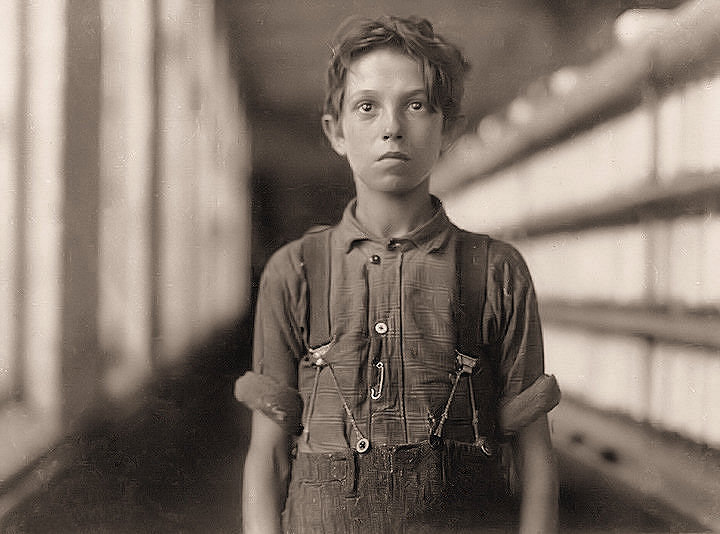
\includegraphics[height=203.5pt, width=5cm, keepaspectratio]{hine02}\hfill}
\vskip1pt
\vskip\baselineskip
\lipsum[1-10]\lipsum
\end{multicols}
\the\textheight\\
\the\paperheight
%%%%%%%%%%%%%   END GENERAL SETTINGS  %%%%%%%%%%%%%%%%%%%%%%%

%\chapter{Captions}


\cxset{section numbering=arabic}

\parindent1em

Captions are very visual and both the text as well as its typography need careful consideration. Most readers will read the captions of figures, before reading the text. We will now in the sections that follow use the caption package to change all the parameters of the caption. This is achieved mainly through one macro, with key value styles.



\DeclareRobustCommand\acaption{\protect\RaggedRight Lorem ipsum caption \protect\ldots.}

\begin{figure*}[h]
\captionsetup{format=plain}
\captionsetup{skip=3pt}
\captionsetup{font=small}
\captionsetup{name=Fig}
\captionsetup[figure]{labelfont=bf,textfont=it}
\RaggedRight
\centering 
\begin{minipage}[t]{90pt}
 \includegraphics[width= 70pt]{./graphics/sudan.jpg}
 \caption{\acaption }
\end{minipage}
\captionsetup{name=Figure}
\begin{minipage}[t]{90pt}
 \includegraphics[width= 70pt]{./graphics/sudan.jpg}
 \caption{\acaption }
\end{minipage}
\captionsetup{name=Fig,labelsep=space}
\begin{minipage}[t]{90pt}
 \includegraphics[width= 70pt]{./graphics/sudan.jpg}
 \caption{\acaption }
\end{minipage}
 \caption{Three boys example (changing the figure name).}
\end{figure*}

\section{Setting the caption options}
To set the caption options we can use the 
\begin{verbatim}
\captionsetup{name=Fig,labelsep=space}
\end{verbatim}

\begin{comment}
%
%\begin{wrapfigure}{R}{0pt}
%     \includegraphics[width=3.5cm]{./graphics/mkulu}
%    \caption{Waterdraagster van M'Kullu. From Reize in Taka (Opper-Nubië)
%        De Aarde en haar Volken, 1873.}
%    \label{fig:shortlabel}
%\end{wrapfigure}
\end{comment}

It is highly recommended to use the \texttt{caption} package to setup the captions of figures. This package developed by Axel Sommerfeldt. offers customization of captions in floating environments such
figure and table and cooperates with many other packages.
Please note: Many document classes already have build-in options and commands
for customizing captions.

And if you are just interested in using the
command \cmd{captionof}, loading of the very small capt-of package is usually sufficient.

For wrapped figures the label name is preferable to be shorter, otherwise it leads to text that is either underfull or overfull. You should also try and use the \cmd{RaggedRight} option of the \pkg{ragged2e} package to hyphenate the ragged right text.



Figure~\ref{fig:shortlabel}, has its label shortened by using ``Fig'' rather than "Figure". I have done this as the space available is narrow. The setup is achieved using the \texttt{caption} package's \verb+\captiosetup+ command. We will use this command to vary, the fonts, numbering, labels, separators and other parameters of the captions.

\section{Adjusting the label\hfill\hfill}%%

Adjusting the label, is achieved by setting the key parameter |name| in  

\begin{teXXX}
\captionsetup{name=Figure}
\end{teXXX}



The figures were typeset by using a different setup style. The first one displays the  label fully, the second uses an abbreviation and the third has a new line, before the caption text is displayed.

\subsection{Fonts}

There are three font options which affects different parts of the caption: One affecting the
whole caption (font), one which only affects the caption label and separator (labelfont) and at least one which only affects the caption text (textfont). You set them up using the options shown in the table below:

\begin{table}[htp]
\centering
\smaller
\caption{Key values for fonts, using the caption package}
\begin{tabular}{ll}
\toprule
normalfont &Normal shape\\
up &Upright shape\\
it &Italic shape \\
sl &Slanted shape\\
sc & \textsc{Small Caps Shape}\\
md &Medium series\\
bf &Bold series\\
rm &Roman family\\
sf &Sans Serif family\\
tt &Typewriter family\\
\bottomrule
\end{tabular}
\end{table}

\emphasis{captionsetup,captionof}
\begin{teXXX}
\captionsetup{name=Figure.}
\captionof{figure}{\acaption}
\end{teXXX}

\begin{figure*}[h]
\captionsetup{skip=3pt}
\captionsetup{font=small}
\captionsetup{name=Fig}
\captionsetup{labelfont=bf,textfont=it}
\RaggedRight
\centering 
\begin{minipage}[t]{90pt}
 \includegraphics[width= 70pt]{./graphics/sudan.jpg}
 \caption{\acaption }
\end{minipage}
\captionsetup{name=Figure}
\begin{minipage}[t]{90pt}
 \includegraphics[width= 70pt]{./graphics/sudan.jpg}
 \caption{\acaption }
\end{minipage}
\captionsetup{name=Fig,labelsep=space}
\begin{minipage}[t]{90pt}
 \includegraphics[width= 70pt]{./graphics/sudan.jpg}
 \caption{\acaption }
\end{minipage}
 \caption{Three boys example (changing the figure name).}
\end{figure*}

\section{Adjusting the Separator}


The separator can be adjusted in a similar manner. The package offers the options, \opt{none}, \opt{colon}, \opt{period}, \opt{space}, \opt{quad}, \opt{newline} and \opt{enddash}.  The various options are illustrated
in \hbox{Figures~18-23}.




\section{skips}

Skips are the amount of vertical space between the caption and the figure. The caption package offers the option
\opt{skip=amount}.\footnote{The standard \LaTeX\ classes article, report and book preset it to \opt{skip=10pt}.} We will now make some recommendations as to how to adjust this spacing.

\medskip

\begin{figure}[htp]
\centering

\captionsetup{name=Photo, labelsep=period, skip=5pt, position=bottom}
\includegraphics[width=\textwidth]{./graphics/damageinspection.jpg}
\caption{Damage Inspection.
A squadron operations officer of the 332d Fighter Group points out a cannon hole to ground crew, Italy, 1945.}
\end{figure}

\medskip

The space between the image and the caption should be approximately half the point size of the text. The photo above had the following settings:


\begin{verbatim}
\captionsetup{name=Photo, labelsep=period,
                    skip=5pt, font=scriptsize,
                    position=bottom}
\end{verbatim}

The \verb+\caption+ command offered by LATEX has a design flaw\footnote{According to Axel Sommerfeldt, \textit{see} the \textit{Caption} documentation.}: The command does not
know if it stands on the beginning of the figure or table, or at the end. Therefore it does
not know where to put the space separating the caption from the content of the figure
or table. While the standard implementation always puts the space above the caption
in floating environments (and inconsistently below the caption in longtables), the
implementation offered by this package is more flexible: By giving the option
\opt{position=bottom}, the package correctly inserts the skip.  You can also try the \opt{position=auto}.
\medskip

The caption of the next photograph follows a more traditional approach found in
\begin{figure}[htp]
\vskip10pt
\centering
\captionsetup{name=Photo, labelsep=period, skip=5pt, position=bottom, textfont=scriptsize, justification=centering}
\includegraphics[width=\textwidth]{./graphics/korea.jpg}

\caption*{\textsc{25th Division Troops Unload Trucks and Equipment}\par
\textit{at Sasebo Railway Station, Japan, for transport to Korea, 1950.}}
\vskip10pt
\end{figure}
many books where, there is no label or number and the text is split into two lines. The first line is a photograph heading and the second line is printed in italics with some explanatory stuff about the photo.

To achieve this result we need to firstly use the \emph{starred} form of the caption command and override the formatting commands of the caption.
\begin{verbatim}
\begin{figure}[htp]
\vskip10pt
\centering
\captionsetup{...}
\includegraphics[width=\textwidth]{filename}
\caption*{\textsc{25th Division Troops Unload Trucks and Equipment}\par
\textit{at Sasebo Railway Station, Japan, for transport to Korea, 1950.}}
\vskip10pt
\end{figure}
\end{verbatim}
You will notice that the photograph is between the lines of the paragraph, so I have added some small skips to arrange proper spacing around it.


To my knowledge, you cannot customize the caption package to get the heading for the caption text. You can define your own command to do so:
\begin{verbatim}
\newcommand\captionx[2]{\par%
     \caption*{\textsc{#1}\newline%
     \textit{#1}}%
}
\end{verbatim}
\newcommand\captionx[2]{\par%
     \caption*{\textsc{#1}\par%
     \textit{#2}}%
}

With photographs you need sometimes to add a "credit" to credit the photographer or even a copyright notice. This is necessary, especially if you have licensed images from an agency. For this I would prefer a simple solution where we
just define an \verb+addcredit+ macro. More customization might be possible, as well as a few setup macros. As an exercise have a look at some publications and see how they handle this type of photographs.

\begin{verbatim}
\newcommand\addcredit[1]{%
   \vspace*{-10.5pt}%
   \scriptsize
   \hfill\hfill
   \textit{Credit: #1}%
}
\end{verbatim}
\providecommand\addcredit[1]{%
 \scriptsize%
 \vspace*{-10.5pt}%
 \hfill\hfill\textit{Credit: #1}%
 \vspace{10pt}
}

The results of the code so farm can be seen in the photograph that follows. The credit has been added and
the text has been centered and styled as required.

The full code is now shown below:

\begin{verbatim}
\begin{figure}[htp]
  \centering
  \captionsetup{skip=0pt,  justification=centering}%
  \includegraphics[width=\textwidth]{./graphics/rosenberg.jpg}%
  \addcredit{U.S. DoD.}%
  \captionx{Assistant Secretary Rosenberg}{talks ...}
\end{figure}
\end{verbatim}

\begin{figure}[htp]
  \centering
  \captionsetup{name=Photo, labelsep=period, skip=0pt, position=top, textfont=scriptsize,    justification=centering}%
\includegraphics[width=\textwidth]{./graphics/rosenberg.jpg}%
\addcredit{U.S. DoD.}%
\captionx{Assistant Secretary Rosenberg}{talks with men of the 140th Medium Tank Battalion during a Far East tour.}
\vspace{10pt}
\end{figure}

It all looks perfect, but there is a snag. If the photo is narrower, there will be nothing to stop it floating past the edge of the photo. This can be corrected by enclosing the commands within a minipage.


\begin{figure}[htp]
\captionsetup{name=Fig., labelsep=period}%
\includegraphics[width=0.97\textwidth]{./graphics/movingup.jpg}%
\addcredit{U.S. DoD.}%
\caption{The effects of the credit going past the edge of the figure. This can be corrected by adding a minipage to hold both commands. }
\end{figure}



\newpage
\pagestyle{empty}
\thispagestyle{empty}
\begin{figure}[htp]
\centering

\captionsetup{name=Photo., labelsep=period}%
   \begin{minipage}[t]{0.48\textwidth}%
      \includegraphics[width=\textwidth]{./graphics/movingup.jpg}%
      \addcredit{U.S. DoD.}%
     \caption{The effects of the credit going past the edge of the figure. This can be corrected by adding a minipage to hold both commands. }
\end{minipage}\hfill\hfill
\begin{minipage}[t]{0.48\textwidth}
      \includegraphics[width=\textwidth]{./graphics/survivors.jpg}%
      \addcredit{U.S. DoD.}%
     \caption{The effects of the credit going past the edge of the figure. This can be corrected by adding a minipage to hold both commands. }
\end{minipage}

 \begin{minipage}[t]{0.48\textwidth}
      \includegraphics[width=\textwidth]{./graphics/img009.jpg}%
      \addcredit{U.S. DoD.}%
     \caption{Engineer Construction Troops in Liberia, July 1942.}
\end{minipage}\hfill\hfill
\begin{minipage}[t]{0.48\textwidth}
      \includegraphics[width=\textwidth]{./graphics/survivors.jpg}%
      \addcredit{U.S. DoD.}%
     \caption{The effects of the credit going past the edge of the figure. This can be corrected by adding a minipage to hold both commands. }
\end{minipage}
 \begin{minipage}[t]{0.48\textwidth}
      \includegraphics[width=\textwidth]{./graphics/img126.jpg}%
      \addcredit{U.S. DoD.}%
     \caption{Marine Reinforcements.
A light machine gun squad of 3d Battalion, 1st Marines, arrives during the battle for ``Boulder City.'' }
\end{minipage}\hfill\hfill
\begin{minipage}[t]{0.48\textwidth}
      \includegraphics[width=\textwidth]{./graphics/img124.jpg}%
      \addcredit{U.S. DoD.}%
     \caption{Brothers Under the Skin, inductees at Fort Sam Houston, Texas, 1953. }
\end{minipage}
\end{figure}
\newpage

Neither the original \tex\ or Plain TeX had any means for captioning. For Knuth this was simply another piece of text to be typeset by means of adding space and inserting some notes to make collation of the works easier.

\begin{teXXX}
{\vskip 2in
\hsize=3in \raggedright
\noindent{\bf Figure 3.} This is the caption to the
third illustration of my paper. I have left two inches
of space above the caption so that there will be room
to introduce special artwork.}
\end{teXXX}
\relax

\endinput NEED TO RESTORE
%%    \begin{macro}
%%    This macro is a helper macro to set the paper height and width
%%    we also save the paper name in its own macro.
%%    \begin{macrocode}
%\gdef\setpapersize@cx#1#2#3{%
%   \gdef\papername{#1}
%   \setlength\paperheight{#2}
%   \setlength\paperwidth{#3}
%   % headheight is common to all so we set it here
%   \setlength\headheight{12\p@}
%  % if pdf we need to set the pageheight and pagewidth
%  \global\pdfpageheight=#2
%  \global\pdfpagewidth=#3
%}
%%    \end{macrocode}
%%    \end{macro}
%%
%%    \begin{macro}
%%    \begin{macrocode}
%\def\setparams@cx#1#2#3{%
%    \def\X{#3}\def\XX{11pt}
%    % 11pt font set it as well
%    \ifx\X\XX
%          \@setfontsize\normalsize\@xipt{13.2}\selectfont%
%          \abovedisplayskip 13.2\p@ \@plus 3\p@ \@minus 3\p@
%          \abovedisplayshortskip \z@ \@plus 3\p@
%           \belowdisplayshortskip 6.6\p@ \@plus 3\p@ \@minus 3\p@
%    \else
%       \def\XX{12pt}
%        \ifx\X\XX
%           \@setfontsize\normalsize\@xiipt\@xivpt\selectfont
%           \abovedisplayskip 14.4\p@ \@plus 3\p@ \@minus 3\p@
%           \abovedisplayshortskip \z@ \@plus 3\p@
%          \belowdisplayshortskip 7.2\p@ \@plus 3\p@ \@minus 3\p@
%       \fi
%    \fi
%    \setlength\headsep{#3}
%    \setlength\footskip{#2}
%    \setlength\topskip{#3}
%    \setlength\maxdepth{0.5\topskip} % need to check
% }
%%    \end{macrocode}
%%    \end{macro}
%%
%%    We now set keys for all the paper sizes  
%\cxset{
%        a4paper/.code=\setpapersize@cx{a4paper}{297mm}{210mm},
%        a5paper/.code=\setpapersize@cx{a5paper}{210mm}{148mm},
%        a6paper/.code=\setpapersize@cx{a6paper}{105mm}{148},
%        b5paper/.code=\setpapersize@cx{b5paper}{250mm}{176mm},
%        letterpaper/.code=\setpapersize@cx{letterpaper}{11n}{8.5in},
%        legalpaper/.code=\setpapersize@cx{legalpaper}{14in}{8.5in},
%        executivepaper/.code=\setpapersize@cx{executivepaper}{10.5in}{7.25in},
%}
%%    the classical dimesions were obtained from the Octavo class
%%    we use mm or in depending on the type of paper standard
%\cxset{foolscap/.code=\setpapersize@cx{foolscap}{171mm}{108mm},
%          crown/.code=\setpapersize@cx{crown}{191mm}{127mm},
%          post/.code=\setpapersize@cx{post}{194mm}{122mm},
%          large post/.code=\setpapersize@cx{large post}{210mm}{137mm},
%          demy/.code=\setpapersize@cx{demy}{222mm}{143mm},
%          medium/.code=\setpapersize@cx{medium}{229mm}{146mm},
%          royal/.code =  \setpapersize@cx{royal}{254mm}{159mm},
%          superroyal/.code=\setpapersize@cx{superroyal}{267mm}{171mm}, 
%          imperial/.code=  \setpapersize@cx{imperial}{279mm}{191mm}}
%%   Lulu paper sizes
%%   http://wepod.wordpress.com/lulu-specs/
%%Manuscript Templates
%%6″ x 9″  US TRADE
%%(15.24cm x 22.86cm)
%%8.5″ x 11″
%%(21.59cm x 27.94cm)
%%Comic, 6.625″ x 10.25″
%%(16.827cm x 26.03cm)
%%Landscape, 9″ x 7″
%%(22.86cm x 17.78cm)
%%Square, 7.5″ x 7.5″
%%(19.05cm x 19.05cm)
%%Pocket Size, 4.25″ x 6.875″
%%(10.8cm x 17.46cm)
%%Royal, 15.6cm x 23.4cm
%%(6.14″ x 9.21″)
%%Crown Quarto, 18.9cm x 24.6cm
%%(7.44″ x 9.68″)
%%A4, 21.0cm x 29.7cm
%%(8.27″ x 11.69″)
%%   Set the parameters that depend on font-sizes
%\cxset{
%        lulu pocketbook/.code=\setpapersize@cx{lulu pocket book}{6.87in}{4.25in},
%	lulu digest/.code=\setpapersize@cx{lulu digest}{8.5in}{5.5in},
%	lulu us trade/.code=\setpapersize@cx{lulu us trade}{9in}{6in},
%	lulu royal/.code=\setpapersize@cx{lulu royal}{9.21in}{6.13in},
%	lulu comic/.code=\setpapersize@cx{lulu comic}{10.25in}{6.625in},
%	lulu crown quarto/.code=\setpapersize@cx{lulu crown}{9.68in}{7.44in},
%	lulu small square/.code=\setpapersize@cx{lulu small}{7.5in}{7.5in},
%	lulu square/.code=\setpapersize@cx{lulu large}{8.5in}{8.5in},
%	lulu landscape/.code=\setpapersize@cx{lulu landscape}{7in}{9in},
%	%lulu large landscape/.code=\setpapersize@cx{lulu large landscape}{}{},
%}
%
%\cxset{
%         10pt/.code=\setparams@cx{6pt}{25pt}{10pt},
%         11pt/.code=\setparams@cx{7pt}{27.5pt}{11pt},
%         12pt/.code=\setparams@cx{8pt}{30pt}{12pt} \@setfontsize\normalsize\@xiipt\@xivpt\selectfont,
%}%
%
%%   we need to set a default size before we determine the
%%   rest of the parameters.
% \cxset{a4paper,10pt}
%
%% does not seem to work
%%\@setfontsize\normalsize\@xiipt\@xivpt\normalsize
%
%%    set a default top margin first
%\def\topmarginauto{%
%\setlength{\topmargin}{0.1\paperheight}
%    \addtolength{\topmargin}{-\headheight}
%    \addtolength{\topmargin}{-\headsep}
%    \addtolength{\topmargin}{-1in}
%}
%
%\topmarginauto
%
%\cxset{topmargin/.code=\setlength{\topmargin}{#1}}
%\cxset{topmargin latex/.code=\topmarginauto}
%\cxset{topmargin latex}
%
%%   \section{Calculation of textwidth}
%%    The calculation of textwidth will depend on the strategy employed to calculate it.
%% \begin{macro}{\textwidth}
%%    Define the width of the text block to 0.7 of the page width, and make
%%    calculations a little easier by adjusting the calculated width to a 
%%    whole number of points.
%%    \begin{macrocode}
%\iffalse
%\setlength{\textwidth}{0.7\paperwidth}
%    \@settopoint\textwidth
%%    \end{macrocode}
%% \end{macro}
%%
%% \begin{macro}{\textheight}
%%    The height of the text block itself is set to 0.7 times the page height. 
%%    This amount is then adjusted to ensure that a whole number of lines makes 
%%    up the text block, and does so exactly.
%%    \begin{macrocode}
%\setlength\@tempdima{0.7\paperheight}
%%    \end{macrocode}
%%    take away the first line, which is a bit shorter than the |\baselineskip|,
%%    \begin{macrocode}
%    \addtolength\@tempdima{-\topskip}
%%    \end{macrocode}
%%    this length may be very close, but just a little too small to accommodate 
%%    one more line, so we add a small amount,
%%    \begin{macrocode}
%    \addtolength\@tempdima{5\p@}
%%    \end{macrocode}
%%    and calculate the number of lines in this length,
%%    \begin{macrocode}
%    \divide\@tempdima\baselineskip
%    \@tempcnta=\@tempdima
%%    \end{macrocode}
%%    The correct textheight comes to the number of lines just calculated, 
%%    multiplied by the height of text lines, |\baselineskip|, and with the 
%%    addition of the |\topskip| we took away initially.
%%    \begin{macrocode}
%    \setlength\textheight{\@tempcnta\baselineskip}
%    \addtolength\textheight{\topskip}
%%    \end{macrocode}
%% \end{macro}
%%
%% \subsubsection{Margin dimensions}
%%     Now that we have set the size of the text block, the amount of space
%%     available for margins is set as well. The remaining white space is divided
%%     in a 1:2 ratio, hence the proportions between margins and text become 1:7:2.
%%
%% \begin{macro}{\evensidemargin}
%% \begin{macro}{\oddsidemargin}
%%    Since we are typesetting books, both even and odd side margins have to be
%%    set.
%%    \begin{macrocode}
%\setlength{\evensidemargin}{0.2\paperwidth}
%\addtolength{\evensidemargin}{-1in}
%\setlength{\oddsidemargin}{0.1\paperwidth}
%\addtolength{\oddsidemargin}{-1in}
%%    \end{macrocode}
%
%\fi
%%% end of octavo algorithm and calculations
%
%%    Define an innermargin to enable easy drawing of parameters
%\newlength\innermargin
%\newlength\lefttrim
%\newlength\bottomtrim
%
%%    The stockheight and stockwidth are used when the paper is to be trimmed
%%    they default to the dimensions for paper width and paper height
%\@ifundefined{stockheight}{\global\newlength\stockheight}{}
%\@ifundefined{stockwidth}{\global\newlength\stockwidth}{}
%\ifdim\stockheight=0pt\addtolength\stockheight{\paperheight}\fi
%   \addtolength\stockheight{0mm}
%%
%\ifdim\stockwidth=0pt\addtolength\stockwidth{\paperwidth}\fi
%   \addtolength\stockwidth{0mm}
%%
%%   We set all the trims to zero to start with.
%\setlength\lefttrim{0mm}
%\setlength\bottomtrim{0mm}
%\setlength\trimtop{0mm}
%\setlength\trimedge{0mm}
%%
%%   
%
%
%%% This is a sidenote without the footnote mark
%%\newcommand\marginnote[2][0pt]{%
%% % \let\cite\@tufte@infootnote@cite%   use the in-sidenote \cite command
%%  %\gdef\@tufte@citations{}%           clear out any old citations
%%  \@tufte@margin@par%                 use parindent and parskip settings for marginal text
%%  \marginpar{\hbox{}\vspace*{#1}\marginparfont@cx\marginparjustification@cx\vspace*{-1\baselineskip}\noindent #2}%
%%  \@tufte@reset@par%                  use parindent and parskip settings for body text
%%  %\@tufte@print@citations%            print any citations
%%  %\let\cite\@tufte@normal@cite%       go back to using normal in-text \cite command
%%}
%
%% This macro has been adapted from the layouts package, it sets the units to be printed
%% in the diagrams.
%\newcommand{\printinunitsof@cx}[1]{%
%  \def\l@yunitperpt{1.0}\def\l@yunits{pt}%
%  \def\l@yta{#1}\def\l@ytb{pt}%
%  \ifx \l@yta\l@ytb
%    \def\l@yunitperpt{1.0}\def\l@yunits{pt}%
%  \else
%    \def\l@ytb{pc}%
%    \ifx \l@yta\l@ytb
%      \def\l@yunitperpt{0.083333}\def\l@yunits{pc}%
%    \else
%      \def\l@ytb{in}%
%      \ifx \l@yta\l@ytb
%        \def\l@yunitperpt{0.013837}\def\l@yunits{in}%
%      \else
%        \def\l@ytb{mm}%
%        \ifx \l@yta\l@ytb
%          \def\l@yunitperpt{0.351459}\def\l@yunits{mm}%
%        \else
%          \def\l@ytb{cm}%
%          \ifx \l@yta\l@ytb
%            \def\l@yunitperpt{0.0351459}\def\l@yunits{cm}%
%          \else
%            \def\l@ytb{bp}%
%            \ifx \l@yta\l@ytb
%              \def\l@yunitperpt{0.996264}\def\l@yunits{bp}%
%            \else
%              \def\l@ytb{dd}%
%              \ifx \l@yta\l@ytb
%                \def\l@yunitperpt{0.9345718}\def\l@yunits{dd}%
%              \else
%                \def\l@ytb{cc}%
%                \ifx \l@yta\l@ytb
%                  \def\l@yunitperpt{0.0778809}\def\l@yunits{cc}%
%%                \else
%%                  \def\l@ytb{PT}%
%%                  \ifx \l@yta\l@ytb
%%                    \def\l@yunitperpt{1.0}\def\l@yunits{PT}% gives problems with pgfmathparse
%%                  \fi
%                \fi
%              \fi
%            \fi
%          \fi
%        \fi
%      \fi
%    \fi
%  \fi
%}
%
%% Define keys to set it
%\cxset{geometry units/.code=\printinunitsof@cx{#1}}
%\cxset{geometry units=pt}
%
%% #1 value in pts
%% default in mm sorry USA.
%% rounding in 1 decimal place
%\def\convert@cx#1{%
%   \pgfmathparse{#1*\l@yunitperpt}
%   %\pgfmathround{\pgfmathresult}
%   \pgfmathresult\thinspace\l@yunits
%}
%
%% Layout related macros to go to separate style file
%\def\aspectratio{\pgfmathparse{\paperheight/\paperwidth} \pgfmathresult}
%
%
%
%
%% Set to true to draw an oddside page. Initially set to false.
%\newcommand\layoutscale@cx{0.4}
%
%\newif\ifoddpagelayout@cx
%   \oddpagelayout@cxtrue
%
%% Set true to draw marginpars on a page
%\newif\ifdrawmarginpars
%   \drawmarginparstrue
%
%% This draws a two page spread
%\newlength\bindingcorrection
%\newlength\oneninth
%\newlength\sixninths
%\setlength\oneninth{\dimexpr(\paperwidth/9)}
%\setlength\sixninths{\dimexpr(\paperwidth*6/9)}
%\let\trytextwidth\sixninths
%
%
%\newcommand{\alphabet}{\normalfont\selectfont\raggedleft abcdefghijklmnopqrstuvwxyz}%82
%
%
%
%\newcommand\charactersperline{%
%  \settowidth{\@tempdima}{\alphabet}
%  \pgfmathparse{\textwidth/\@tempdima*26}
% \pgfmathprintnumber{\pgfmathresult}
%}
%
%\newcommand\alphabetsperline{
%  \settowidth{\@tempdima}{\alphabet}
%  \pgfmathparse{\textwidth/\@tempdima}
%  \pgfmathresult
%}
%
%\newlength\alphlength
%\newcommand\alphabetlength{%
%  \settowidth{\alphlength}{\alphabet}
%  \pgfmathparse{\alphlength}
%  \pgfmathprintnumber{\pgfmathresult}pt
%}
%
%% We need to use the fp package to calculate the ratios, as PGF has problems with large 
%% dimensions or I am making an error
%\newcommand\textarearatio{%
%    \FPmul{\result}{\strip@pt\textwidth}{\strip@pt\textheight}
%    \FPmul{\resulti}{\strip@pt\paperwidth}{\strip@pt\paperheight}
%    \FPdiv{\resultii}{\result}{\resulti}
%    \pgfmathprintnumber{\resultii}
%}
%
%% Calculate the ratio textheight/paperheight
%\newcommand\textheightratio{%
%    \FPdiv{\result}{\strip@pt\textheight}{\strip@pt\paperheight}
%    \FPround{\result}{\result}{2}
%    \result
%}
%
%% Calculate textheight/paperwidth
%
%\newcommand\textheighttopaperwidth{%
%    \pgfmathparse{\textheight/\paperwidth}
%    \pgfkeys{/pgf/number format/.cd,fixed,precision=2}
%    \pgfmathprintnumber{\pgfmathresult}
%}
%
%\newlength\margintop
%
%\newcommand\thetop{%
%   \pgfmathparse{1in+\topmargin+\headheight+\headsep}
%   \pgfmathsetlength{\margintop}{\pgfmathresult}
%}
%
%\thetop
%
%\newlength\marginbottom
%\newcommand\thebottom{%
%   \pgfmathparse{\stockheight-(1in+\topmargin+\headheight+\headsep+\textheight)}
%    \pgfmathsetlength{\marginbottom}{\pgfmathresult}
%  }
%\thebottom
%
%\newcommand\verticalmarginratio{%
%\pgfmathparse{(\paperheight-(1in+\topmargin+\headheight+\headsep+\textheight))/  (\paperheight-(1in+\topmargin+\headheight+\headsep+\textheight))}
%\pgfmathresult
%}
%
%\newcommand\horizontalmarginratio{%
%\pgfmathparse{(\paperwidth-\textwidth-\oddsidemargin)/(1in+\oddsidemargin)}
%\pgfmathresult
%}
%
%\newcommand\numbertextlines{%
%% baselineskip to be corrected
%   \pgfmathparse{(\textheight-\topskip)/(12)-1}\pgfmathresult
%}
%
%\cxset{geometry units=mm}
%
%\def\printgeometryvalues{%
%   \noindent
%   \begin{tabular}{ll}
%   paper name & \papername\\
%   stock height & \convert@cx{\stockheight}\\
%   stock width  & \convert@cx{\stockwidth}\\
%   paperwidth & \convert@cx{\paperwidth}\\
%   paperheight & \convert@cx{\paperheight}\\
%   voffset & \convert@cx{\voffset}\\
%   hoffset & \convert@cx{\hoffset}\\
%   thetextheight & \convert@cx{\textheight}\\
%   thetextwidth  & \convert@cx{\textwidth}\\
%   Top margin   &  \thetop\convert@cx{\the\margintop}\\  % need to correct
%   Bottom margin & \thebottom\\
%   thetopmargin & \convert@cx{\topmargin}\\
%   theheadheight & \convert@cx{\headheight}\\
%   theheadsep & \convert@cx{\headsep}\\
%   theoddsidemargin & \convert@cx{\oddsidemargin}\\
%   theevensidemargin & \convert@cx{\evensidemargin}\\
%   themarginparsep& \convert@cx{\marginparsep}\\
%   themarginparwidth& \convert@cx{\marginparwidth}\\
%   themarginpush& \convert@cx{\marginparpush}\\
%   thevoffset& \convert@cx{\voffset}\\
%   thefootskip& \convert@cx{\footskip}\\
%   aspect ratio \aspectratio\\
%   twoside&  \if@twoside true\else false\fi\\
%   reversemarginpar& \if@mparswitch true \else false\fi\\
%  \end{tabular}
% }
%
%\def\readability{%
%\begin{tabular}{lr}
%  Characters per line &\charactersperline\\
%  Alphabets per line &\alphabetsperline\\
%  Alphabet length &\alphabetlength\\
%  Baselineskip & \the\baselineskip\\
%  Number of text lines &\numbertextlines\\
%  Text area ratio &\textarearatio\\
%  textheight/paperwidth&\textheighttopaperwidth\\
%  Text/page height ratio & \textheightratio\\
%  Vertical margin ratio &\verticalmarginratio\\
%  Horizontal margin ratio &1:\horizontalmarginratio\\
%\end{tabular}}
%
%
%% Note with new geometry paper has to be defined in preamble
%% I do not feel very confident of this
%% Don't understand it fully how is working
% %\@twosidefalse \@mparswitchfalse % one side option
%%\cxset{geometry oxford/.code={
%%\newgeometry{left=74.8mm,top=27.4mm,headsep=2\baselineskip,%
%%marginparsep=8.2mm,marginparwidth=49.4mm,textheight=49\baselineskip,headheight=\baselineskip}
%%\@twosidefalse \@mparswitchfalse % one side option
%%\reversemarginpar
%%}}
%% \@mparswitchfalse
%%\cxset{geometry textwidth/.store in=\textwidth@cx,
%%          geometry textheight/.store in=\textheight@cx,
%%          geometry tufte/.code={
%%             \newgeometry{a4paper,left=24.8mm,top=27.4mm,headsep=2\baselineskip,%
%%             textwidth=107mm,marginparsep=8.2mm,marginparwidth=49.4mm,%
%%             textheight=\textheight@cx\baselineskip,headheight=\baselineskip}
%%            \@twosidefalse \@mparswitchfalse % one side option
%%           %\reversemarginpar
%%    }
%%}
%%
%%
%%\cxset{marginpar push/.store in=\marginparpush@cx,
%%          marginpar font/.store in=\marginparfont@cx,
%%          marginpar justification/.is choice,
%%          marginpar justification/justifying/.code=\gdef\marginparjustification@cx{\justifying},
%%          marginpar justification/raggedright/.code=\gdef\marginparjustification@cx{\raggedright},
%%          marginpar justification/RaggedRight/.code=\gdef\marginparjustification@cx{\RaggedRight},
%%          marginpar justification/RaggedLeft/.code=\gdef\marginparjustification@cx{\RaggedLeft},
%% }
%%%\cxset{marginpar push=10pt,
%%%          marginpar font=\normalfont\footnotesize\sffamily,
%%%          marginpar justification=RaggedLeft}
%%%
%%%
%%%\cxset{style13, geometry textheight=47,
%%%          %geometry tufte,
%%%          watermark text=SAMPLE TUFTE VARIANT,
%%%          watermark text color=thered,
%%%          header style=samplepage}
%%%%%%%%%%%%%%%%%%%%%
%
%%%%%%%%%%%%%%%%%%%%%%%%%%%%%%%%%%%%%%%%%%%%%%%%%%%%%%%%%%%%%%%%%%%%%%%%%%
%%    DRAW THE PAGE ON A TRIAL BASIS
%%
%%%%%%%%%%%%%%%%%%%%%%%%%%%%%%%%%%%%%%%%%%%%%%%%%%%%%%%%%%%%%%%%%%%%%%%%%%%
%
%\cxset{geometry units= in}
%% lots of keys for trial sizes. We default all sizes to the ones defined in
%% by the document class.
%
%% We first set keys for the vertical dimensions
%\newlength\trytextheight@cx
%\newlength\tryheadheight@cx
%\newlength\tryheadsep@cx
%\newlength\tryfootskip@cx
%
%% LaTeX uses a correction to adjust the top margin, which is called topmargin. It does not 
%% represent the top margin though which following geometry we denote as top. It could perhaps
%% better be called top margin correction
%
%\newlength\trytopmargin@cx
%
%% Set keys for all the vertical dimensions and default to the current document settings
%\cxset{try textheight/.code=\global\setlength\trytextheight@cx{#1},
%          try textheight/.default=\textheight,
%          try headheight/.code=\global\setlength\tryheadheight@cx{#1},
%          try headheight/.default=\headheight,
%          try headsep/.code=\global\setlength\tryheadsep@cx{#1},
%          try headsep/.default=\headsep,
%          try footskip/.code=\global\setlength\tryfootskip@cx{#1},
%          try footskip/.default=\footskip,
%          try topmargin/.code=\global\setlength\trytopmargin@cx{#1},
%          try topmargin/.default=\topmargin,
%}
%
%% Set keys for all the trims, different people have different names for them. Normally two trims are
%% specified the top trim and the edge trip. We define two others just in case and to make calculations
%% easier if we have to use a different stock paper from the actual virtual paper width. the virtual
%% paper is called the paperwidth and paperheight.
%
%% We need to pick-up the memoir and koma allowances. TODO!
%\newlength\trimtop@cx
%
%\cxset{try trimtop/.code=\global\setlength\trimtop@cx{#1},
%          try trimtop/.default=\global\setlength\trimtop{0pt},}
%
%% set all the defaults
%
%\cxset{try textheight,
%          try headheight,
%          try headsep,
%          try footskip,
%          try topmargin=0pt, % compensate for trim
%          try trimtop=0pt}
%
%\addtolength\trytopmargin@cx{0pt}
%
%% set horizontal keys
%\newlength\trytextwidth@cx
%\setlength\trytextwidth@cx{0pt}
%\newlength\trytrimedge@cx
%\setlength\trytrimedge@cx{0pt}
%
%\cxset{try textwidth/.code=\global\setlength{\trytextwidth@cx}{#1},
%          try trimedge/.code=\global\setlength{\trytrimedge@cx}{#1},
%}
% 
%\cxset{try textwidth=\textwidth,
%          try trimedge=0pt}
%
%\def\alignedge{%
%% removed parindent from here must add it at the image
%  \checkoddpage%
%%   \ifoddpage \global\setlength\innermargin{\oddsidemargin}
%%          \else \global\setlength\innermargin{\evensidemargin}
%%      \fi%
%%   \if@twoside\setlength\innermargin{\dimexpr(\evensidemargin-\marginparsep)}%
%%             \else\let\innermargin\oddsidemargin\fi
%   \ifoddpage 
%      \innermargin\oddsidemargin
%      \def\innermarginname{oddsidemargin}%
%     \else
%        \innermargin\evensidemargin
%        \def\innermarginname{evensidemargin}%
%  \fi
%  }
%
%\alignedge
%
%
%%\ifoddpage
%%  \addtolength\innermargin{50pt}
%%\else
%%  \addtolength\innermargin{20pt}
%%\fi
%%\addtolength\trytextheight@cx{-20pt}
%%\addtolength\trytextwidth@cx{-24pt}
%%\addtolength\marginparwidth{-24pt}
%
%\reversemarginparfalse
%
%\def\drawlayout{%
%  \checkoddpage
%   \alignedge
%
%\tikzset{dim/.style = {>= latex,color=black}}
%\begin{tikzpicture}[scale=0.45,font={\scriptsize\rmfamily},line width=.8pt,
%       every node={color=black}]
%
%% first we draw stockwidth and stockheight
%\draw [color=gray,fill=thegray] (0,0) rectangle ++(\stockwidth,\stockheight);
%
%% draw the paper 
%\ifoddpage
%  \draw [color=NavyBlue,dashed thick,fill=white]  (0+\lefttrim,\stockheight-\trimtop@cx) rectangle ++ 	(\stockwidth-\lefttrim-\trytrimedge@cx,-\stockheight+\trimtop@cx+\bottomtrim);
%\else
% \draw [color=NavyBlue,dashed thick,fill=white]  (0+\lefttrim+\trytrimedge@cx,\stockheight-\trimtop@cx) rectangle ++ (\stockwidth-\lefttrim-\trytrimedge@cx,-\stockheight+\trimtop@cx+\bottomtrim);
%\fi
%% dimensions one more try
%%\cxset{geometry units=mm}
%% paper width dimensions, better to change to a macro
%% tol is the distance to dimension
%
%% paper width
%\edef\tol{-2.5\baselineskip}
%\coordinate (A) at (0+\lefttrim,\tol);
%\coordinate (B) at (\stockwidth-\trimedge,\tol);
%\coordinate (C) at (0.5\stockwidth,\tol);
%\draw[dim, |<->|] (A) -- (B); 
%\node at (C) [yshift=0.5\baselineskip)]{paper width = \convert@cx{\paperwidth}};
%
%% stockwidth
%\edef\tol{-5\baselineskip}
%\coordinate (BD) at (0,\tol);
%\coordinate (BD2) at (\stockwidth,-5\baselineskip);
%\draw[dim, |<->|] (BD) -- (BD2); 
%\draw (BD) ++ (0.5\stockwidth,0) node [yshift=0.5\baselineskip]{stockwidth=\convert@cx{\stockwidth}} ;
%
%% top dimension at left
%\coordinate (H1) at (-5mm,\stockheight);
%\coordinate (H2) at (-5mm,\stockheight-1in-\trytopmargin@cx-\tryheadsep@cx-\tryheadheight@cx);
%\draw [dim,|<->|] (H1) -- (H2);
%\node[left,text width=1.5cm, text ragged left] at (-5mm,\stockheight-0.5*\margintop){top\\ \convert@cx{\the\margintop}};
%
%% bottom dimension at left
%\coordinate (H3) at (-5mm,0);
%\coordinate (H4) at (-5mm,\marginbottom);
%\draw [dim,|<->|] (H3) -- (H4);
%\node[left] at (-5mm,0.5*\marginbottom){\convert@cx{\the\marginbottom}};
%
%% textheight at left
%\draw[dim,<->]  (-5mm, \marginbottom) -- ++ (0,\trytextheight@cx);
%\node[left,text width=1.5cm,text ragged left] at (-5mm,\marginbottom+0.5\trytextheight@cx){textheight \convert@cx{\trytextheight@cx}};
%
%
%% trimedge
%\ifoddpage
%  \coordinate (D) at (\stockwidth-4\trimedge, 0.10\trytextheight@cx);
%  \coordinate (E) at (\stockwidth,0.10\trytextheight@cx);
%  \draw [dim,->|] (D) -- ++(3\trimedge,0);
%  \draw [dim,|<-|] (E) -- ++(3\trimedge,0) node at ++(0,0) [right,text width=2cm,color=black] {trim edge    \convert@cx{\the\trimedge}};
%\else
%%  \coordinate (D1) at (\trytrimedge@cx, 0);
%%  \coordinate (E1) at ++ (\trytrimedge@cx,\stockheight-\trimtop@cx);
%%  \draw (D1)--(E1);
%\fi
%
%
%% toptrim
%%\ifdim\trimtop>0pt
%  \coordinate (F) at (0.9\stockwidth, \stockheight-\trimtop@cx-8mm);
%  \coordinate (G) at (0.9\stockwidth, \stockheight-\trimtop@cx);
%  \coordinate (H) at (0.9\stockwidth,\stockheight);
%  \draw (F)[dim,->|] -- (G);
%  \draw (H) -- ++ (0,8mm) -- ++ (5mm,0)[|<-|,>=latex] 
%          node [right] at ++ (0,0) {top trim =  \convert@cx{\the\trimtop@cx}};
%%\fi
%
%% 1in offsets
%\draw[dashed,color=gray] (1in,0) -- (1in,\stockheight);
%\draw[dashed,color=gray] (0in,\stockheight-1in)-- ++ (\stockwidth,0);
%
%% oddsidemargin/evensidemargin
%% draw dimension and name based on even or odd page
%\draw[dim,|<->|] (0,0.1\trytextheight@cx) -- ++(1in+\innermargin,0) node[right] at ++ (2ex,0) [text width=2cm] {\innermarginname\  \convert@cx{\the\innermargin}};
%
%% HEADER
%\coordinate (I) at (1in-\lefttrim+\innermargin,\stockheight-1in-\tryheadheight@cx-\trytopmargin@cx+\trimtop@cx);
%\draw (I) rectangle ++ (\textwidth,\tryheadheight@cx);
%
%%\draw[dim,<->] (1.5in\tol,\stockheight) -- ++(0,-1in) node[above right] at ++ (0,0.2in) {1in + yoffset};
%
%% add in inch 
%\draw [dim,|-|] (\stockwidth+3ex,\stockheight-\trimtop@cx)
%      -- ++(0,-1in) node [right] at ++(2ex,0.65in) {offset=\convert@cx{1in}};
%
%%   add topmargin dimension
%\ifdim\topmargin>0pt
%\draw [dim,|-] (\stockwidth+3ex,\stockheight-1in+\trimtop@cx)
%      -- ++(0,-\trytopmargin@cx) node [right] at ++(2ex,0.5\trytopmargin@cx) {topmargin=\convert@cx{\topmargin}};
%\fi
%
%%  add headheight dimension
%\draw [dim,|-|] (\stockwidth+3ex,\stockheight-1in+\trimtop@cx-\trytopmargin@cx)
%        -- ++(0,-\tryheadheight@cx) node [right] at ++(2ex,0.5\tryheadheight@cx) {headheight=\convert@cx{\the\tryheadheight@cx}};
%
%%   add headsep dimension
%\draw [dim,|-] (\stockwidth+3ex,\stockheight-1in+\trimtop-\tryheadsep@cx-\tryheadheight@cx-\trytopmargin@cx)
%          -- ++(0,\tryheadsep@cx) node [below right] at ++(2ex,0){headsep = \convert@cx{\the\tryheadsep@cx}};
%
%% footskip dimension
%\draw [dim,|-|] (\stockwidth+3ex,\stockheight-1in+\trimtop@cx-\tryheadsep@cx-\tryheadheight@cx-\trytopmargin@cx-\trytextheight@cx) -- ++(0,-\tryfootskip@cx) node [right] at ++(2ex,0.5\tryfootskip@cx){footskip=\convert@cx{\the\tryfootskip@cx}};
%
%
%% textarea
%\coordinate (J) at (1in-\lefttrim+\innermargin-\trytrimedge@cx,\stockheight-1in+\trimtop@cx-\tryheadheight@cx-\trytopmargin@cx-\tryheadsep@cx-\trytextheight@cx);
%\draw[fill=lightgray!50] (J) rectangle ++ (\trytextwidth@cx,\trytextheight@cx);
%
%\draw[dim,<->|] (1in-\lefttrim+\innermargin,0.75\trytextheight@cx) -- ++(\trytextwidth@cx, 0)  node at ++(-0.5\trytextwidth@cx,0.5\baselineskip) {textwidth} node at ++ (-0.5\trytextwidth@cx,-\baselineskip) {\convert@cx{\the\trytextwidth@cx}};
%
%\pgfmathsetmacro{\gridx}{12}
%% draw grid
%\draw[xstep=(\paperwidth-\trimedge)/\gridx, ystep=(\stockheight-\trimtop@cx)/\gridx,color=gray,dotted]  (0,0) grid (\paperwidth,\paperheight); 
%%%   add textheight dimension
%%\draw [dim,-] (\stockwidth+3ex,\stockheight-1in+\trimtop-\headsep-\headheight-\topmargin) -- ++(0,-\textheight) node [right] at ++(2ex,0.5\textheight){textheight=\convert@cx{\the\textheight}};
%
%% footer
%\coordinate (I) at (1in-\lefttrim+\innermargin,  \stockheight-1in+\trimtop@cx-\tryheadheight@cx-\trytopmargin@cx-\tryheadsep@cx-\trytextheight@cx-\tryfootskip@cx);
%\draw (I) rectangle ++ (\trytextwidth@cx,\tryheadheight@cx);
%
%
%% marginpar
%\def\leftmarginpar{%
%    \draw [fill=Linen,opacity=0.7] (1in+\innermargin+\trytextwidth@cx+\marginparsep,   \stockheight-1in+\trimtop@cx-\trytopmargin@cx-\tryheadsep@cx-\tryheadheight@cx ) rectangle ++(\marginparwidth,-\trytextheight@cx);
% \draw [dim,|<->|] (1in-\lefttrim+\trytextwidth@cx+\innermargin+\marginparsep+\marginparwidth,0.75\trytextheight@cx) -- ++ (-\marginparwidth,0) node at ++(0.5\marginparwidth,0.5\baselineskip) {marginpar} node at ++(0.5\marginparwidth,-\baselineskip){\convert@cx{\the\marginparwidth}};
%}
%
%\def\rightmarginpar{%
% \draw [color=red] (1in+\innermargin-\marginparsep,\stockheight-1in+\trimtop@cx-\trytopmargin@cx-\tryheadsep@cx-\tryheadheight@cx ) rectangle ++(-\marginparwidth,-\trytextheight@cx);
%     \draw [dim,|<->|] (1in-\lefttrim+\innermargin-\marginparsep-\marginparwidth,0.75\trytextheight@cx) -- ++ (\marginparwidth,0) node at ++(-0.5\marginparwidth,0.5\baselineskip) {marginpar} node at ++(-0.5\marginparwidth,-\baselineskip){\convert@cx{\the\marginparwidth}};
%}
%
%\ifdrawmarginpars
%  \checkoddpage
%  \alignedge
%    \if@twoside
%         \ifoddpage
%            \leftmarginpar
%         \else
%            \rightmarginpar
%        \fi
%   \else
%  % one side paper
%        \leftmarginpar
%    \fi
%\fi
%
%% draw diagonal
%\ifoddpage
%     \draw [color=blue]  (\paperwidth-\trytrimedge@cx,0) -- (0, \stockheight-\trimtop@cx);
%  \else
%    \draw [color=blue] (\trytrimedge@cx,0) -- (\paperwidth,\paperheight-\trimtop@cx);
%\fi  
%\end{tikzpicture}
%}
%
%
%%%%%%%%%%%%%%%%%%%%%%%%%%%%%%%%%%%%%%%%%%%%%%%%%%%%%%%%%%%%%%%%%%
%%                 SPREAD DRAWN AS PER CLASSICAL RULES
%%                 FOR ILLUSTRATION PURPOSE
%%%%%%%%%%%%%%%%%%%%%%%%%%%%%%%%%%%%%%%%%%%%%%%%%%%%%%%%%%%%%%%%%%%
%\newlength\paperwidth@cx
%\newlength\paperheight@cx
%\setlength\paperwidth@cx{6in}
%\setlength\paperheight@cx{9in}
%\setlength\bindingcorrection{0.1in}
%
%\def\spread{%
%   \begin{tikzpicture}[scale=0.5,inner sep=0pt,outer sep=0pt]
%   % draw the two pages
%  
%   \draw[xstep=\paperwidth@cx/9,ystep=\paperheight@cx/9,color=blue] (0,0) rectangle (\paperwidth@cx,\paperheight@cx)  (\paperwidth@cx+\bindingcorrection,0) rectangle ++(\paperwidth@cx,\paperheight@cx);
%
%% draw the binding correction
%\draw[fill=gray, draw] (\paperwidth@cx,0)  rectangle (\paperwidth@cx+\bindingcorrection,\paperheight@cx);
%
%% draw grid
%
%\draw[xstep=(\paperwidth@cx)/9, ystep=(\paperheight@cx)/9,color=gray,]  (0,0) grid (\paperwidth@cx,\paperheight@cx);
%
%\draw[xstep=(\paperwidth@cx)/9, ystep=(\paperheight@cx)/9,color=red]  
%(6.2in,0) grid (12.2in,\paperheight@cx);
%
%% add type areas
%
%\draw[fill=purple] (2\paperwidth@cx/9,2\paperheight@cx/9) rectangle  ++(6/9*\paperwidth@cx,6*\paperheight@cx/9);
%
%\draw[fill=green] (\paperwidth@cx+\paperwidth@cx/9+\bindingcorrection,2\paperheight@cx/9) rectangle ++(6\paperwidth@cx/9,6\paperheight@cx/9);
%
%\ifdim\bindingcorrection>0pt
%\draw[color=white,font={\sffamily\bfseries}] node at (\paperwidth@cx+0.5\bindingcorrection, 0.5\paperheight@cx)[rotate=90,inner sep=0pt,outer sep=0pt] {BINDING CORRECTION};\fi
%
%\node [color=white,font={\sffamily\bfseries}] at (0.5\paperwidth,0.5\paperheight)  {LEFT PAGE};
%\node [color=white,font={\sffamily\bfseries}] at (1.5\paperwidth@cx+\bindingcorrection,0.5\paperheight@cx){RIGHT PAGE};
%
%% draw diagonals
%
%\draw [color=thegreen, line width=1.5pt] (0,0)-- (\paperwidth@cx,\paperheight@cx);
%\draw [color=thegreen, line width=1.5pt] (2\paperwidth@cx+\bindingcorrection,0)-- ++(-\paperwidth@cx,\paperheight@cx);
%
%% draw circles
%
%\draw [color=red] (0.5\paperwidth@cx,5\paperheight@cx/9) circle (0.5\paperwidth@cx);
%
%\end{tikzpicture}
%}
%
%
%
%

\chapter{Geometry and Page Dimensions}
\parindent1.5em

\section{Introduction}

Setting up the page geometry, is normally done by the class or if adjustments need to be made, most authors will use the package geometry. If you need to view the geometry and the values of the document layout you can use the pkg{layouts}. This package offers a set of convenience key values for setting up geometry in order to enable authors to have a comprehensive style sheet.

\section{How to set geometry via this package}

To set the geometry page of the whole document, set the keys in the preamble. To change the page geometry anywhere in the document use the appropriate style or keys where you want the page geometry to change.
Note that the paper zize can only be defined in the preamble. The package is more useful when loaded with predefined styles.

\begin{tcolorbox}
\begin{lstlisting}
\cxset{page geometry=medieval}
\end{lstlisting}
\end{tcolorbox}

In most instances you will want to load the geometry at the style sheet.


\section{Viewing the page geometry}

The package offers a number of keys to set documents either document wide or locally to change page 
parameters or to view the frames. this is very similar to what the layouts and geometry packages offer. We do
however use TikZ for these diagrams.

To incorporate a layouts diagram we offer two macros \cs{printlayout} and \cs{printlayoutvalues}. Both have associated styling keys.
\medskip

\section{The Ideal Page Layout}

Since the invention of writing, typographers, scribes and graphics artists have been on the quest to find the ideal
layout for a page. Figure~\ref{fig:medieval}, shows a probablee geometric method that was used to typeset such books as the Gutenburg bible. Tschischold was a major revivalist of the method. Since most measurements in those times were probably only done using a compass a ruler and possibly a square, dividing the page equally into a nine part grid was done by first drawings the diagonals that are shown in blue in the figure, the intersections were then determined from the red lines thus enabling the typed area to be demarcated. 


\begin{figure}[htbp]
\pgfmathsetmacro\xsteps{9}
\pgfmathsetmacro\ysteps{9}
\cxset{spread scale=0.3}
\drawclassicspread
\caption{The ideal medieval page spread.}
\label{fig:medieval}
\end{figure}

To the modern eye, pages typeset in this manner might look rather empty, so smadjustments are made to such layuots. However, one tries to keep the proportions approximately to those of the classical layouts.
 
\begin{figure}[htbp]
  \includegraphics[width=0.95\textwidth]{tchichold01}
  \caption{\protect\url{http://www.artlebedev.com/everything/izdal/novaya-tipografika/}}
\end{figure}

\section{Technical discussion}
\subsection{The LaTeX standard classes}

LaTeX has pre-build layouts that depend  on two variables, specified by the user: the \textit{paper size} and the \textit{font size}. Appropriate values for the rest of the page layout are then  calculated by the class algorithm or are preset to certain values.

\subsection{Other common classes}

The more generic classes such as memoir and koma-script offer extensive customization and calculation of page parameters. They all use the basic laTeX page terminology which they supplement for additional parameters.

The octavo class offers a set of paper sizes suited for classical layouts printed on classical sizes such as the octavo. Classes such as the tufte-book offer a fixed design and no special commands for parameter manipulation.

\subsection{Paper sizes}

Most people using LaTeX, will print on either a4paper or letterpaper sizes. If you going to bind the work it might be necessary to trip the paper a little bit during binding to make sure that the top and side of the book are not ragged. This is normally called the \textit{trim}. If the document is to be printed by a publishing house this might be done by the printer which will use a different size \textit{stock size}. They might also allow for two additional dimensions called the spinemargin or the foremargin.

\begin{table}[ht]
\caption{North American paper sizes.}
\begin{tabular}{lllll}
\toprule
Size &width (mm)  &Height (mm)  &Width (in) &Height (in)\\
\midrule
US Ledger   &432 &279 & 17.0 &11.0\\
US Tabloid &279 & 432 & 11.0 &17.0\\
US Letter  &216 & 279 & 8.5 &11.0\\
US Legal   &216 &356 & 8.5 & 14.0\\
Government Letter &203 & 267 & 8.0 &10.5\\
Junior Legal &203 & 127 & 8.0 & 5.0\\
\bottomrule
\end{tabular}
\end{table}

\clearpage

\begin{table}[ht]
\caption{A series paper sizes.}
\begin{tabular}{lllll}
\toprule
Size &width (mm)  &Height (mm)  &Width (in) &Height (in)\\
\midrule
A0   &841 &1189 &33.1 & 46.8\\
A1   &594 & 841 &23.4 & 33.1\\
A2   & 420 & 594 &16.5 &23.4\\
A3   &297 & 420 &11.7 &16.5\\
A4   &210 &297 &8.3 &11.7\\ 
A5   &148 & 210 &5.8 & 8.3\\
A6   &105 & 148 & 4.1 & 5.8\\
A7   & 74 & 105 & 2.9 & 4.1\\
A8   &52 & 74 & 2.0 & 2.9\\
A9   &37 & 52 & 1.5 & 2.0\\
A10  & 26 & 37 & 1.0 & 1.5\\
\bottomrule
\end{tabular}
\end{table}


\begin{table}[ht]
\caption{ANSI series paper sizes.}
\begin{tabular}{lllll}
\toprule
Size &width (mm)  &Height (mm)  &Width (in) &Height (in)\\
\midrule
ANSI A &216 &279 &8.5 &11.0\\
ANSI B &279 &432 &11.0 &17.0\\
ANSI C &432 &559 &17.0 &22.0\\
ANSI D &559 &864 &22.0 &34.0\\
ANSI E &864 &1118 &34.0 &44.0\\

\bottomrule
\end{tabular}
\end{table}

\clearpage

\section{Swedish Standard}
The Swedish standard SIS 014711 generalized the ISO system of A, B, and C formats by adding D, E, F, and G formats to it. Its D format sits between a B format and the next larger A format (just like C sits between A and the next larger B). The remaining formats fit in between all these formats, such that the sequence of formats A4, E4, C4, G4, B4, F4, D4, H4, A3 is a geometric progression, in which the dimensions grow by a factor 21/16 from one size to the next. However, the SIS 014711 standard does not define any size between a D format and the next larger A format (called H in the previous example). Of these additional formats, G5 and E5 are popular in Sweden for printing dissertations,but the other formats have not turned out to be particularly useful in practice and they have not caught on internationally.

\begin{table}[ht]
\caption{Swedish Extension}
\begin{tabular}{lllll}
\toprule
Size &width (mm)  &Height (mm)  &Width (in) &Height (in)\\
\midrule
G5 &169 &239 &6.65 &9.41\\
E5  &155 &220 &6.10 &8.66\\

\bottomrule
\end{tabular}
\end{table}


\begin{table}
\centering
\caption{Octavo page layout parameters, influenced by font-size}
\begin{tabular}{llll}
\toprule
                    & 10pt & 11pt &12pt \\
\midrule
\textit{Octavo}              &      &      &\\
headsep        &  6pt  &  7pt &  8pt\\
topskip          & 10pt &  11pt & 12pt\\
texwidth         &0.7paperwidth & &\\
\midrule
\textit{LaTeX}              &      &      &\\
headsep        & .25in   &  .275in & .275in \\
topskip          & 10pt &  11pt & 12pt\\
footskip         &.35in &  .38in & 30pt \\
maxdepth         &.5\textbackslash topskip & &\\
textwidth        & 345pt  & 360pt & 390pt\\
\bottomrule
\end{tabular}
\end{table}

\subsection{The page dimensions}

The page dimensions are shown in figure 1. We tried to cater for the common terminology of all the classes.

\subsection{Texwidth}

The width of the text can only be determined based on the designer's strategy and is inexorably tied also to
the textheight. For example in classical page design, the designer tried to get the textwidth to be the same size like the page width, thus giving an almost squarish look. Another strategy is the 6-9 strategy, where the paper is divided into a grid of 9 equal blocks and the textwidth occupies the 6. 

\subsection{Readability considerations}

An average line that is longer than 40 to 70 characters long -- inluding spaces, is difficult to read. This is generally applicable to European languages and might be different for other languages. In addition the average number of words in one line should also be considered. For the German language Willi Egger (2004) recommends a line consisting of 8 to 12 words as optimal. If this strategy is adopted one can determine the line length based on the number of letters.

The characters per line for this document is \charactersperline. Of course from a readabilty point of view one could keep increasing the font size, but this is poor strategy. A well designed page should allow for good proportions as well as readabilty. In general a tolerance up  to 80 characters on a line should be adequate.

Peter Wilson in the manual for the memoir class refers to equations developed by Morten H{\o}gholm\index{H{\o}gholm, Morten} that has done some curve fitting
to the data. He determined that the expressions
\begin{equation}
L_{65} = 2.042\alpha + 33.41 \label{eq:L65}
\end{equation}
and
\begin{equation}
L_{45} = 1.415\alpha + 23.03 \label{eq:L45}
\end{equation}
fitted aspects of the data, where $\alpha$ is the length of the alphabet
in points, and $L_{i}$ is the suggested width in points, for a line with
$i$ characters (remember that 1pc = 12pt).

Using these equations one could get a first estimate of the textwidth. I am not too sure though if this is a good strategy as one can calculate it fully using TeX. bringhurst and them had to read these values from tables, but we do not; we can easily calculate them. For example to calculate the alphabet length for the bookman font:

\begin{texexample}{}{}
  \bgroup
  \fontfamily{pbk}\selectfont\alphabetlength\\
  \charactersperline\\
  \the\textwidth
  \egroup
\end{texexample}

Table~\ref{tab:alphlengths} adapted from the memoir class, gives alphabet lengths in points for various
fonts. My own recommendation is that for wide paper you should use a wider font and possibly move to 11pt font, rather than the traditional LaTeX default of 10pt.

\begin{table}
\centering
\caption{Lowercase alphabet lengths, in points, for various fonts}\label{tab:alphlengths}
\begin{tabular}{lrrrrrrrr} \toprule
                                            & 8pt & 9pt & 10pt & 11pt & 12pt & 14pt & 17pt & 20pt \\ \midrule
\fontfamily{pbk}\selectfont Bookman         & 113 & 127 & 142 & 155 & 170 & 204 & 245 & 294 \\
\fontfamily{bch}\selectfont Charter         & 102 & 115 & 127 & 139 & 152 & 184 & 221 & 264 \\
\fontfamily{cmr}\selectfont Computer Modern & 108 & 118 & 127 & 139 & 149 & 180 & 202 & 242 \\
\fontfamily{ccr}\selectfont Concrete Roman  & 109 & 119 & 128 & 140 & 154 & 185 & 222 & 266 \\
\fontfamily{pnc}\selectfont New Century Schoolbook     & 108 & 122 & 136 & 149 & 162 & 194 & 234 & 281 \\ 	
\fontfamily{ppl}\selectfont Palatino        & 107 & 120 & 133 & 146 & 160 & 192 & 230 & 276 \\ 	
\fontfamily{ptm}\selectfont Times Roman     &  96 & 108 & 120 & 131 & 143 & 172 & 206 & 247 \\
\fontfamily{put}\selectfont Utopia          & 107 & 120 & 134 & 146 & 161 & 193 & 232 & 277 \\
\fontfamily{pag}\selectfont Avant Garde Gothic  & 113 & 127 & 142 & 155 & 169 & 203 & 243 & 293 \\
\fontfamily{cmss}\selectfont Computer Sans  & 102 & 110 & 120 & 131 & 140 & 168 & 193 & 233 \\
\fontfamily{phv}\selectfont Helvetica       & 102 & 114 & 127 & 139 & 152 & 184 & 220 & 264 \\
\fontfamily{pcr}\selectfont Courier         & 125 & 140 & 156 & 170 & 187 & 224 & 270 & 324 \\
\fontfamily{cmtt}\selectfont Typewriter     & 110 & 122 & 137 & 149 & 161 & 192 & 232 & 277 \\
\bottomrule
%\facesubseeidx{Bookman}\facesubseeidx{Charter}\facesubseeidx{Computer Modern}%
%\facesubseeidx{Concrete Roman}\facesubseeidx{New Century Schoolbook}
%\facesubseeidx{Palatino}\facesubseeidx{Times Roman}\facesubseeidx{Utopia}%
%\facesubseeidx{Avant Garde Gothic}\facesubseeidx{Computer Sans}
%\facesubseeidx{Helvetica}\facesubseeidx{Courier}%
%\facesubseeidx{Computer Typewriter}%
\end{tabular}
\end{table}

\subsection{Textwidth influenced by margin materials}

Many books, including LaTeX allow for margin materials. If this is true then of course margins must by their nature be larger at the paper edges to allow for such material. 

\subsubsection{Simple strategy}
However, despite most of the above typesetting strategies many an author just want to take an approach, where they specify the margins and want to get what they need for example a spine margin of 1cm and an edge margin of 1.5cm. This is also important for screen dimensions.

\begin{lstlisting}
\cxset{
    margin inner= 1in
    margin outer= 2in
    margin top=1in
    margin bottom=2in
}
\end{lstlisting}

If all four margins are specified, the typesetting area can be positioned on the paper block. Life is not this easy though.

\begin{lstlisting}
\cxset{
    textarea proportional={1}{6}{2}  %
    textarea octavo
    textarea latex
    textarea other
}
\end{lstlisting}

\subsection{Auto strategy}

A more involved approach is to combine the strategies. First to get a good margin to type area, you will need to choose a paper that has good ratios. A paper such as \textit{imperial} comes close to an A4 size or imperial size. One can trip the balance of the paper or adjust slightly the ratios for twoside printing. Since we talking about book design any consideration for one side printing is immaterial. For oneside printing one can accept a wider latitude of values. Algorithm follows:

\begin{enumerate}
\item select paper.
\item select font.
\item marginmaterial true or false.
\item financial constraints - minimize number of pages, maximize number of pages.
\item check ideal number of characters at 65 per line.
\item decide on 10pt, 11pt or 12pt and constrain the algorithm.
\item use 0.7 textwidth area and check for max characters, if not iterate to 11pt.
\item recommend trimming values to suit.
\end{enumerate}


\subsection{Textheight}
Normally there is more latitude in choosing the 
proportions\index{proportion!margin} 
of the upper and lower margins, though usually the upper 
margin\index{margin!upper} is less than the lower margin\index{margin!lower}
so the typeblock\index{typeblock!location} is not vertically centered. Many modern books disregard all these rules and in many examples the upper margin is higher than the lower margin.

For text height calculations there are two considerations. One is to select top and bottom margings that are either equal or at a 1:1.5--2.0 ratio and relate to the width of the horizontal margins. The second consideration is that this length must be exactly divisible by baselineskip. When using \cs{flushbottom} LaTeX expects that the \cs{textheight} is such that a number of textlines in the body font will fit exactly into the height. If not, it issues an underfull vbox's message. LaTeX calculates these parameters when loading the class .clo files and sets the number of lines to a round number.

Many modern books have equal upper and lower margins.
\bigskip

\section{Allowing for trims}

Once a book is printed the edges are trimmed a bit in order to ensure a smooth top and right edge. For most desktop publishing you should not worry about such trimming. If you are going to publish the book in a professional publisher get their advice as to any allowances, you need to make in your pdf file. In other possible scenarios is that you may want to use a paper size such as A4 and trim it yourself down to one of the classical sizes such as Royal. 

All calculations are based on selecting a paper size and trimming it down. Unlike some other classes we assume you have selected the paper as stock size and then trimmed. Adding the trims makes no sense. You could simply print them on the larger page with trim marks, which we cater for.

  \begin{align}
   H_p    & = \sum h_1\ldots h_n\\
      h_t  &= H_p -   \sum h_1\ldots h_n - h_b
  \end{align}

The top margin is influenced by the \textit{device margin}, which is set at one inch, which we denote as $C$. If paper is to be trimmed the effective device margin offset will be reduced by the trim amount, $\Delta_t$.

Hence, the top margin is given by
\begin{align}
     h_t = C-\Delta_t+h1+h_2+h_3
\end{align}


\drawtriallayout


\printgeometryvalues
\readability

\newpage

\drawtriallayout

\readability

\newpage



% end of two page spread
\subsection{Top and bottom margins}

Before you follow any advice in places such as the Lulu forums to have your top and bottom margins equal, consider the following quotation by Bernard Shaw:

\begin{quotation}
Every printer can understand regularity: few have studied good looks except in living creatures. Consequently they aim at equal margins; and even when they have learnt that an upper margin must be less than a lower one if it is not to look more, they do not always see that it looks well only when it looks less. The mediaeval manuscript or early printed book, with its very narrow margin at the top and very broad margin at the bottom of the page, with its outer margins broad and its inner ones contracted, so that when the book lies open the two pages seem to make but a single block of letterpress in a single frame, instead of two side by side, has never been improved upon and probably never will be. But I find it almost impossible to persuade a modern printer to make his top margin small enough; and when I at last succeed, he measures it from the running title instead of from the top line of the page.

I saw a book the other day, excellently printed in old faced type, set solid, on a fine light, clean white crusty paper; yet the page was quite spoiled by an exaggerated top margin,like a masher's collar, and by that abomination of desolation, a rule. The only thing that never looks right is a rule. There is not in existence a page with a rule on it that cannot be instantly and obviously improved by taking the rule out.
\end{quotation}

\subsection{Headers and footers}
A page may have two additional items, and usually has at least one of these. They are the
running header and running footer. If the page has a folio then it is located either in the
header or in the footer. The word ‘in’ is used rather lightly here as the folio may not be
actually in the header or footer but is always located at some constant relative position. A
common position for the folio is towards the fore-edge of the page, either in the header or
the footer. This makes it easy to spot when thumbing through the book. It may be placed
at the center of the footer, but unless you want to really annoy the reader do not place it
near the spine.

Often a page header contains the current chapter title, with perhaps a section title on
the opposite header, as aids to the reader in navigating around the book. Some books put
the book title into one of the headers, usually the verso one, but I see little point in that as
presumably the reader knows which particular book he is reading, and the space would
be better used providing more useful signposts.

\subsubsection{Determining the geometry of the headers and footers}

The important parameter in the calculation of the header and footers, is the \cs{headheight} and \cs{headsep}. Most classes tend to have these as fixed parameters, related to font-size as can be seen in Table~\ref{tab:headerparams}.

\begin{table}[htbp]
\centering
\caption{Header and footer parameters settings by common classes.}
\label{tab:headerparams}
\begin{tabular}{llll}
\toprule
                    &headsep                   &headheight &footskip\\
\midrule
LaTeX 10pt    &             &                 &           \\
LaTeX 11pt    &             &                 &           \\
LaTeX 12pt    &             &                 &           \\
Octavo          &             &                 &           \\
tufte-book     &2 \texttt{baselineskip}   & 1 baselineskip           &            \\
\bottomrule
\end{tabular}
\end{table}

\begin{figure}[htbp]
\includegraphics[width=\textwidth]{paradoxicalbrain}

\caption{Modern book approach to footer and header design. From \textit{Paradoxical Brain,} Narinder Kapur \textit{et al.}, Cambridge Univerity Press, 2011. Book is printed on Royal size paper.}
\label{fig:paradoxical}
\end{figure}

\begin{figure}[htbp]
{{\parindent0pt
\begin{tikzpicture}[inner sep=0pt,outer sep=0pt]
  \node (img) {\includegraphics[height=8cm]{paradoxicalbrain}};
  \draw  (img.north east) ++ (5pt,0pt)-- ++ (15pt,0) ++(-15pt, -0.083*8cm) --++ (15pt,0pt) 
            (img.south east) ++ (5pt,0pt) -- ++ (15pt,0pt) ++ (0,0.075*8cm) -- ++ (-15pt,0);
\end{tikzpicture}}}
\caption{Modern book approach to footer and header design. From \textit{Paradoxical Brain,} Narinder Kapur \textit{et al.}, Cambridge Univerity Press, 2011. Book is printed on Royal size paper. The top margin is $1/12$ of the page height and the bottom margin is $1/16$ of page height. No need for apogryphal methods here.}
\label{fig:paradoxical}
\end{figure}

The more modern style tends to shift the headers and footers towards the top edge and bottom edge of the paper respectively, and allows very little space at the top of the paper. Figure~\ref{fig:paradoxical} shows a footer that is very near the bottom of the text and a header that has been shifted upwards. This makes for a more economical design as it increases the amount of text that can be printed in the typed area. For special designs such as this, it is not possible to automate calculations other than specifying a full algorithm for margins and typed area. Margins for the example follow the 10/12 rule for the typed area and inner and outer margins are equal at 1:12 ratio to the trimmed paper width.


\section{Floating parameters}


\section{Summing up}

Although one would ideally like to input some constraints and get out a perfect layout, as the previous discussion shows this is not an easy task, as well 

\begin{figure}[htbp]
\includegraphics[width=0.9\textwidth]{artbook}
\end{figure}

%%\end{document}
%\lipsum[1-4]\marginnote[1pt]{\lorem
%    \lorem}
%
%\lipsum[1-2]

%% Stick the caption in the head might as well place the first picture also
\def\asidecaption{\parbox{4.2cm}{{\bfseries Image \thefigure}\par\lorem}%
  % \addtocontents{lof}{This is image 8}
}
\def\ps@caption{%
     \let\@oddfoot\@empty\let\@evenfoot\@empty%
    \def\@evenhead{%
        \begin{picture}(0,0)%
           \put(-150,-80){\asidecaption\par}%
            \stepcounter{figure}
           \put(-150,-370){\asidecaption}%
        \end{picture}%
      }%
    \let\@oddhead\@evenhead%
    \let\@mkboth\@gobbletwo%
    \let\chaptermark\@gobble%
    \let\sectionmark\@gobble%
 }

\def\ps@bigpicture{%
    \setlength\headheight{19cm}%
    \let\@oddfoot\@empty\let\@evenfoot\@empty%
    \def\@evenhead{%
         \begin{picture}(0,0)%
          \put(-149,0){\includegraphics[width=\dimexpr(\textwidth+150pt)]{stuartpearson}}%
         \end{picture}%
      }%
    \let\@oddhead\@evenhead%
    \let\@mkboth\@gobbletwo%
    \let\chaptermark\@gobble%
    \let\sectionmark\@gobble%
 }



\def\doubletakeimage{%
  \renewcommand{\topfraction}{.95}  % ensure seecond image will not float away
  \begin{figure}[t]
    \thispagestyle{caption}
    \includegraphics[width=\textwidth]{matron}%
  \end{figure}

  \begin{figure}[tp]
   \hspace*{-\marginparwidth}\includegraphics[height=0.9\textheight]{stuartpearson}
 \end{figure}
}




\lipsum[1-4]
\begin{figure}[htp]
\includegraphics[width=0.98\textwidth]{captionspecial}
\centering
\caption{Figure from \textit{Oxford History of Art, Portraiture}, Shearer West, Oxford University Press, 2004. The figures are numbered consecutively and the text in the List of Illustrations have different formatting.}
\end{figure}

\doubletakeimage



%% RESET EVERYTHING AT END OF CHAPTER
\addtocounter{chapter}{-2}

\@toctrue\@specialtrue

\@specialfalse
\pdfpageheight=\paperheight
\pdfpagewidth=\paperwidth
\cxset{manet, toc image=false}
\cxset{toc image=false},
\topimage{manet}

\chapter{THE BARMAID}
\begin{multicols}{3}
      \leftskip0pt
      \lettrine{I}{psum dolor} sit amet latixeus. \lipsum*[1-2]
      Latinicus porcupinus to fill the line.
      \tikz{\draw[thick] (0,0)--(\columnwidth,0);}
\end{multicols}
\clearpage


%\cxset{manet, toc image=false}
%\cxset{toc image=false},
%\topimage{Alan-MacDonald-Cardinal-Spin-01}
%\chapter{THE BARMAID}
%\begin{multicols}{3}
%      \leftskip0pt
%      \lettrine{I}{psum dolor} sit amet latixeus. \lipsum*[1-2]
%      Latinicus porcupinus to fill the line.
%\end{multicols}
%\clearpage

\restoregeometry
\@specialfalse


\newgeometry{top=1.35cm,bottom=2cm,left=2cm}
\clearpage
\cxset{manet/.style={
 chapter opening=anywhere,
 chapter toc=true,
 toc image=false,
 name={},
 numbering=none,
 number font-size=,
 number font-family=,
 number font-weight=,
 number before={\vspace*{-2.5cm}},
 number dot={},
 number after={},
 number position=leftname,
 chapter font-family=,
 chapter font-weight=,
 chapter font-size=,
 chapter before=,
 chapter after={},
 chapter color={black!90},
 number color= teal,
 title beforeskip={},
 title afterskip={},
 title before={\hspace*{-2.47cm}\includegraphics[width=1.27\textwidth]{./chapters/manet}%
    \par\hfill\hfill{\tiny\bfseries Manet's  \textit{The Barmaid.}}\\
    \par
    \vspace*{\baselineskip}
    \par\hfill},
 title after={\hfill\hfill},
 title font-family=\sffamily,
 title font-color= black!80,
 title font-weight=\bfseries,
 title font-size=\LARGE}}
\cxset{manet}



\chapter{A New Approach to Designing \LaTeX\ Classes}
\begin{multicols}{3}
      \leftskip0pt
      \lettrine{I}{psum dolor} sit amet latixeus. \lipsum*[1-2]
      Latinicus porcupinus to fill the line.


This particular code, uses the predefined style \textit{manet}. The only difference we have now defined a helper macro to make it easier for such images to be inserted for similar style chapter openings.
If a full book is to be designed using chapter openings in this fashion more keys and styles could be defined to make it even more easy to enter.
\end{multicols}



\def\topimage#1{\cxset{title before={\hskip-2.3cm\includegraphics[width=1.25\textwidth]{./chapters/#1}\par
\vspace*{\baselineskip}\par}}}




The full code to have the chapter typeset is shown below:


\begin{lstlisting}
\cxset{manet}
\topimage{Alan-MacDonald-Cardinal-Spin-01}

\chapter{ALAN MacDONALD}
\begin{multicols}{3}
      \leftskip0pt
      \lettrine{I}{psum dolor} sit amet latixeus. \lipsum*[1-2]
      Latinicus porcupinus to fill the line.
\end{multicols}
\end{lstlisting}
\lipsum[2]

\loadgeometry{std}



\cxset{toc image=false},

\long\gdef\versochapter#1{%
  \vspace*{3cm}
  \minipage{\textwidth}
  \hfill\includegraphics[width=0.63\textwidth]{\chapterimage@cx}\par
  \vspace*{6pt}
  \hfill\minipage{0.75\textwidth}
  {\HUGE\bfseries\flushright #1\endflushright}
  \endminipage
  \endminipage
  \newpage


\vspace*{10cm}
\@specialfalse
\@openleftfalse
\@openanyfalse
\@openrighttrue
}


\newgeometry{bottom=2.5cm}

\cxset{
   chapter image/.code={\def\chapterimage@cx{#1}},
   chapter opening/.is choice,
   chapter opening/verso/.code={\@specialtrue\@openlefttrue
   \gdef\customdesign@cx##1{\versochapter{##1}}}
}

\cxset{
 chapter image=onesowndeath,
 chapter opening=verso,
 name={},
 numbering=none,
 number font-size=\LARGE,
 number font-family=\rmfamily,
 number font-weight=\bfseries,
 number before=,
 number dot=,
 number after=,
 number position=leftname,
 chapter font-family=\sffamily,
 chapter font-weight=\normalfont,
 chapter font-size=\Large,
 chapter before={\vspace*{0pt}\par},
 chapter after={\hfill\hfill\par},
 chapter color={black!90},
 number color=\color{purple},
 title beforeskip={\vspace*{0pt}},
 title afterskip={\vspace*{0.4\textheight}\par},
 title before={},
 title after={},
 title font-family=\sffamily,
 title font-color=\color{purple},
 title font-weight=\bfseries,
 title font-size=\LARGE,
 header style=plain,
 pagestyle=plain,
 }

\@specialtrue

\chapter[VERSO CHAPTERS]{Verso Chapters}

\parindent1.5em
{\HUGE V}erso chapter openings are not common. One design that I found quite attractive is \lipsum[1-3] \textit{From Western attitudes toward death from the middle ages to the present}, Philippe Ari\'es. London, 1974.

\begin{figure}
\includegraphics[width=\textwidth]{versochapter01}
\caption{Chapter opening on verso page.}
\end{figure}


%\makeatletter\@specialfalse

\cxset{
 toc image = \@empty,
 name={},
 numbering=arabic,
 number font-size= LARGE,
 number font-family= rmfamily,
 number font-weight= bfseries,
 number before=,
 number dot=,
 number after=,
 number position=leftname,
 chapter font-family= sffamily,
 chapter font-weight= normalfont,
 chapter font-size= Large,
 chapter before={\vspace*{15pt}\par},
 chapter after={\hfill\hfill\par},
 number color=black!90,
 title beforeskip={\vspace*{30pt}},
 title afterskip={\vspace*{40pt}\par},
 title before={},
 title after={},
 title font-family= sffamily,
 title font-color= black,
 title font-weight= bfseries,
 title font-size= LARGE,
 header style= plain,
 }

\cxset{headings ruled-01}

\chapter{Introduction to Style One}


\begin{summary}
This design is simple and its distinguishing characteristic is a short summary at the beginning of the chapter. This is almost like an abstract typeset in italic font without setting the margins in. We provide a \lstinline{summary} environment for convenience. Note the very simple line in the running head to the left of the page number.
\end{summary}

\medskip
\begin{figure}[ht]
\centering
\includegraphics[width=0.5\textwidth]{./chapters/chapter01.png}
\end{figure}
\makeatother

%\clearpage
\makeatletter\@debugtrue\makeatother
\cxset{
 chapter toc=true,
 name=CHAPTER,
 chapter numbering=ORDINALS,
 number font-size=Large,
 number font-family=rmfamily,
 number font-weight=bfseries,
 number before=\kern0.5em,
 number dot=,
 number after=\hfill\hfill\par,
 number position=rightname,
 chapter font-family=rmfamily,
 chapter font-weight=bold,
 chapter font-size=Large,
 chapter before={\vspace*{20pt}\par\hfill},
 chapter after=,
 chapter color=black,
 number color=black,
 %
 title margin top=10pt,
 title before=\par\nointerlineskip\hfill,
 title after=\hfill\hfill\par\nointerlineskip,
 title font-family=rmfamily,
 title font-color= black,
 title font-weight=bfseries,
 title font-size=LARGE,
 chapter title width=0.8\textwidth,
 chapter title align=centering,
 title margin-left=0pt,
 author block=false}

\debugtitle
\debugchapter
\chapter[Template 2]{Mondino, the Restorer of Anatomy}

The archive.org is an extraordinary hunting ground  for typographical surprises. On a recent excursion to find some books on Versalius I stubled on a book titled \emph{Andreas Vesalius, the reformer of anatomy} by  Ball, James Moores. It is an old book published in 1910 and has a couple of unusual features. Check the figure below and see if you can identify the challenging feature.

\begin{figure}[ht]
\centering
\includegraphics[width=0.8\textwidth]{versalius}
\caption{J.B. Moore’s \emph{Andreas Versalius, the Reformer of Anatomy} has many unusual features, including chapter numbers using ordinals. }
\end{figure}

\cxset{chapter toc=true,
          chapter opening=anywhere}
          
\chapter{The Template}          
The template is called \emph{Versalius} and is stored under style02. It can be loaded in the normal way using:
\begin{verbatim}
\usepackage[style02]{phd}
\end{verbatim}

I have not reproduced the full extend of the book’s requirements, as some details are quite cumbersome to be automated through \tex. These though can easily be incorporated in a manual way. More about this later.


\section{The Table of Contents}
Another interesting aspect of this book, which is common with many books of its period is the ToC. The ToC shows the full range of the chapter pages, i.e., it is marked as Page 1-16 rather than the common practice nowdays that indicates only the starting page of the chapter. It also has “TABLE OF CONTENTS”  as a heading and not just contents as you would expect from today’s books.

\begin{figure}[ht]
\centering
\includegraphics[width=0.8\textwidth]{versalius-01}
\caption{J.B. Moore’s \emph{Andreas Versalius, the Reformer of Anatomy} has many unusual features, including chapter numbers using ordinals. }
\end{figure}

\section{List of Illustrations}

\begin{figure}[ht]
\centering
\includegraphics[width=0.8\textwidth]{versalius-02}
\caption{J.B. Moore’s \emph{Andreas Versalius, the Reformer of Anatomy} has many unusual features, including chapter numbers using ordinals. }
\end{figure}

\section{The Frontmatter}
As a foreward there is an unumbered chapter called ``Introduction’’. The chapter heading also has a head band.
\begin{figure}[ht]
\centering
\includegraphics[width=0.8\textwidth]{versalius-03}
\caption{J.B. Moore’s \emph{Andreas Versalius, the Reformer of Anatomy} has many unusual features, including chapter numbers using ordinals. }
\label{lettrine}
\end{figure}

\bgroup
\centering
\includegraphics[width=0.7\textwidth]{versalius-headband}

\LARGE\bfseries INTRODUCTION\par
\egroup
\def\dropcapversalius{%
\vbox to 0pt{\vskip6pt\leavevmode\noindent\includegraphics[width=2.39cm]{versalius-dropcap}%
}%
}
\parindent0pt

\hangindent2.6cm \hangafter0
\dropcapversalius \textsc{he dropcap will have to be inserted}, either using the lettrine package or do be achieved via a parshape command and manual entry. You can also write your own macro command using the details we provide under the Paragraphs chapter. On this page I have manually inserted it, as I used an image from the book for the dropcap. If you were to use the template for a full book, it will be then preferable to use

the lettrine package to set the dropcaps. If you observe Figure~\ref{lettrine} carefully, you will notice the first line of theopening paragraph is in small caps. As \tex typesets the full paragraph this is almost an impossible task to achieve through normal \tex commands and in order not to overcomplicate the discussion it can be achieved manually via trial and error. 

\section{Figures}

Most of the figures are wrapped illustrations. A couple are full page figures and bear no caption numbering. One such illustration is shown on page~\pageref{fig:vesalius}. Do note that the List of Illustrations does have the illustrations listed with additional information to that shown in the captions. 

\begin{figure}[p]
\centering
\includegraphics[width=\textwidth]{vesalius}
\centering
ANDREAS VESALIUS\par
(From an old copperplate engraving)\par
\label{fig:vesalius}
\end{figure}







%\newgeometry{top=-10pt,bottom=2cm}


\cxset{style03/.style={
 toc image = \@empty,
 name={},
 numbering=arabic,
 number font-size= HUGE,
 number font-family= rmfamily,
 number font-weight= bfseries,
 number before=\par\vspace*{10pt}\hfill\hfill,
 number dot=.,
 number after=,
 number position=rightname,
 chapter font-family= sffamily,
 chapter font-weight=normalfont,
 chapter font-size= Large,
 chapter before={\hspace*{-2.5cm}\vbox\bgroup%
    \tcbset{width=\paperwidth,boxrule=0pt,right=3cm,arc=0pt}
    \tcolorbox\bgroup\vspace*{20pt}\hfill\hfill},
 chapter after={\par\vspace*{15pt}},
 chapter color=black!90,
 number color= thered,
 title beforeskip={},
 title afterskip={\vspace*{10pt}\par},
 title before={\hfill\hfill},
 title after={\vspace*{60pt}\egroup\endtcolorbox\egroup},
 title font-family=\sffamily,
 title font-color= thered,
 title font-weight=\bfseries\RaggedRight,
 title font-size=\Huge}}

\cxset{style03}

\chapter{Introduction Style Three}

This is not an exact reproduction as I am still thinking as to how to use
specials with the package. You can vary it by setting the tcolorbox settings as well as the geometry settings.
\medskip

\begin{figure}[ht]
\centering
\includegraphics[width=0.39\textwidth]{./chapters/chapter03}
\end{figure}

This setting involves changing the geometry of the page as well as adding the chapter name and title in a color box. For this I have used the \lstinline{tcolorbox}. Of course you can use any other shaded environment you feel comfortable with such as mdframed. It is important to set the colorbox parameters.

\begin{lstlisting}
\newgeometry{top=-10pt}
\tcbset{width=\paperwidth,boxrule=0pt,right=3cm,arc=0pt}
\end{lstlisting}

Note that we set the width of the \lstinline{tcolorbox} to \lstinline{\paperwidth} in order for the shading to extend to the full width of the page.

\restoregeometry

%\cxset{style04/.style={
 chapter name=,
 numbering=Roman,
 number font-size=Large,
 number font-family=rmfamily,
 number font-weight=bfseries,
 number before=,
 number dot=,
 number after=,
 number color=black,
 number position=rightname,
 chapter font-family= rmfamily,
 chapter font-weight=bold,
 chapter font-size=Large,
 chapter before=,
 chapter after=,
 chapter color=black!90,
 chapter border-style=none,
 chapter border-width=0pt,
 chapter display=block,
 chapter float=center,
 title beforeskip={},
% title afterskip={\vspace*{50pt}\par},
 title margin bottom=50pt,
 title margin-left=0pt,
 chapter title align=centering,
 chapter title text-align=center,
 chapter title width=\textwidth,
 title display=block,
 title border-left-width=0.2pt,
% title hooks leave emptt 
 title before=,
 title after=,
 % title families leave as default font name
 title font-family=rmfamily,
  title font-color= black,
 title font-weight=normalfont,
 title font-size=LARGE,
 % title alignment
 chapter title align=centering,
 % sectioning incomplete please add to suit
 section numbering=none,
 section align = center}}

\debugchapter
\cxset{chapter border-width=2pt,
          chapter padding=5pt,
          number border-width=2pt,
          number padding=5pt}

\cxset{style04}

\chapter{INTRODUCTION TO STYLE FOUR}

This is a very simple design applicable perhaps to translations and commentary on older texts.
\medskip
\begin{figure}[ht]
\centering
\includegraphics[width=0.6\textwidth]{./chapters/chapter04.png}
\end{figure}

\testsections



%%%%%%%%%%%%%%%%%%%%%%%%%%%%%%%%%%%%%%%%%%%%
%%%%%%  STYLE 05
%%%%%%%%%%%%%%%%%%%%%%%%%%%%%%%%%%%%%%%%%%%


\cxset{style05/.style={
 name={Chapter},
 numbering=arabic,
 number font-size=\Large,
 number font-family=\rmfamily,
 number font-weight=\normalfont\itshape,
 number color=\color{black!90},
 number before=,
 number dot=,
 number after=,
 number position=rightname,
 chapter font-family=\rmfamily,
 chapter font-weight=\normalfont\itshape,
 chapter font-size=\Large,
 chapter before={\hrule width \columnwidth \kern2.6pt \par\hfill},
 chapter after={\hfill\hfill\par},
 chapter color={black!90},
 chapter spaceout=none,
 title beforeskip={\vspace*{10pt}},
 title afterskip={\vspace*{50pt}\par},
 title before={\hfill},
 title after={\hfill\hfill \vskip2.6pt\hrule width \columnwidth \kern2.6pt },
 title font-family=\rmfamily,
 title font-color=\color{black!90},
 title font-weight=\bfseries,
 title font-size=\huge,
 header style= headings}}

\cxset{style05}
\chapter{Introduction to Style Five}\index{ch:style5}

\tcbset{width=\textwidth}
I think this style can be improved with a bit of color. You can experiment with it quite easily. The spacing on top of this style can also be adjusted to suit your typographical taste.
\medskip
\begin{figure}[ht]
\centering
\includegraphics[width=0.6\textwidth]{./chapters/chapter05}
\end{figure}

%\section{General notes on rules}

LaTeX's default rules would normally give problems. Best is to use TeX's primitives to built them.

%\index{rules!example color}
%\begin{texexample}{}{}
%\makeatletter
%\hrule width 5cm \kern2.6\p@
%AAAAAAAAAAAAAAAAAAAAA
%\vskip2.6pt\hrule width 5cm
%\medskip
%
%Problem with LaTeX rules.
%
%\rule{5cm}{0.4pt}\par
%AAAAAAAAAAAAAAAAAAAAA\par%
%\rule[6.5pt]{5cm}{0.4pt}
%
%\def\rule{\@ifnextchar[\@rule{\@rule[\z@]}}
%\def\@rule[#1]#2#3{%
% \leavevmode
% \hbox{%
% \setlength\@tempdima{#1}%
% \setlength\@tempdimb{#2}%
% \setlength\@tempdimc{#3}%
% \advance\@tempdimc\@tempdima%
% \vrule\@width\@tempdimb\@height\@tempdimc\@depth-\@tempdima}}
%
%\def\thickrule{\leavevmode \leaders \hrule height 3pt \hfill \kern \z@}
%
%{\color{teal}\hrule width 10.5cm height3pt \kern2.6\p@
%    {{\color{black!80}\HUGE CHAPTER TITLE}}\vskip3pt
%\hrule width 10.5cm height3pt}
%\makeatother
%\end{texexample}

%<<<<<<< HEAD
%%%%%%%%%%%%%%%%%%%%%%%%%%%%%%%%%%%%%%%%%%%
%%%%%%  STYLE 06
%%%%%%%%%%%%%%%%%%%%%%%%%%%%%%%%%%%%%%%%%%%

\cxset{style06/.style={
 name={Chapter},
 numbering=arabic,
 number font-size=\Huge,
 number font-family=\calligra,
 number font-weight=\calligra,
 number color=\color{black!90},
 number before=\kern-2.5pt,
 number dot=,
 number after=,
 number position=rightname,
 chapter font-family=\rmfamily,
 chapter font-weight=\calligra,
 chapter font-size=\LARGE\calligra,
 chapter before={\vspace*{20pt}\par\hfill},
 chapter after={\hfill\hfill\par},
 chapter color={black!90},
 title beforeskip={\vspace*{50pt}},
 title afterskip={\vspace{3.5pt}\par},
 title before={\hfill},
 title after={\hfill\hfill},
 title font-family=\rmfamily,
 title font-color=\color{black!90},
 title font-weight=\normalfont,
 title font-size=\LARGE,
 title spaceout=soul,
}}

\cxset{style06}

\chapter{INTRODUCTION TO STYLE SIX}
\renewcommand{\DefaultLhang}{0.1}
\renewcommand{\LettrineFontHook}{\calligra}
\setlength{\DefaultFindent}{9.5pt}
\setlength{\DefaultNindent}{0pt}

\lettrine{\textcolor{orange}{T}}{}he calligraphic font for this design make it stand out, although you may need to experiment to get the right font (I have used calligra). I am sure the specification can be optimized a bit, however so far it works. I also opted to space out the title. I had to experiment a bit to get the Lettrine settings.
\medskip
\begin{figure}[ht]
\centering
\includegraphics[width=0.6\textwidth]{./chapters/chapter06}
\end{figure}

The number has been kerned using:

\begin{lstlisting}
 number before=\kern-4.5pt,
\end{lstlisting}

This template has a lot of potential and I will come back to it and add more key hooks for lettrine settings per letter and font management. They can also come alive with a gold color.

=======
%%%%%%%%%%%%%%%%%%%%%%%%%%%%%%%%%%%%%%%%%%%
%%%%%%  STYLE 06
%%%%%%%%%%%%%%%%%%%%%%%%%%%%%%%%%%%%%%%%%%%

\cxset{style06/.style={
 name={Chapter},
 numbering=arabic,
 number font-size=\Huge,
 number font-family=\calligra,
 number font-weight=\calligra,
 number color=\color{black!90},
 number before=\kern-2.5pt,
 number dot=,
 number after=,
 number position=rightname,
 chapter font-family=\rmfamily,
 chapter font-weight=\calligra,
 chapter font-size=\LARGE\calligra,
 chapter before={\vspace*{20pt}\par\hfill},
 chapter after={\hfill\hfill\par},
 chapter color={black!90},
 title beforeskip={\vspace*{50pt}},
 title afterskip={\vspace{3.5pt}\par},
 title before={\hfill},
 title after={\hfill\hfill},
 title font-family=\rmfamily,
 title font-color=\color{black!90},
 title font-weight=\normalfont,
 title font-size=\LARGE,
 title spaceout=soul,
}}

\cxset{style06}

\chapter{INTRODUCTION TO STYLE SIX}
\renewcommand{\DefaultLhang}{0.1}
\renewcommand{\LettrineFontHook}{\calligra}
\setlength{\DefaultFindent}{9.5pt}
\setlength{\DefaultNindent}{0pt}

\lettrine{\textcolor{orange}{T}}{}he calligraphic font for this design make it stand out, although you may need to experiment to get the right font (I have used calligra). I am sure the specification can be optimized a bit, however so far it works. I also opted to space out the title. I had to experiment a bit to get the Lettrine settings.
\medskip
\begin{figure}[ht]
\centering
\includegraphics[width=0.6\textwidth]{./chapters/chapter06}
\end{figure}

The number has been kerned using:

\begin{lstlisting}
 number before=\kern-4.5pt,
\end{lstlisting}

This template has a lot of potential and I will come back to it and add more key hooks for lettrine settings per letter and font management. They can also come alive with a gold color.

>>>>>>> merged

%
\newgeometry{top=2cm,bottom=2cm,left=3cm,right=3cm}

\setdefaults

\cxset{style07/.style={
 name={},
 chapter toc=true,
 numbering=arabic,
 number font-size=HUGE,
 number font-family=sffamily,
 number font-weight=bfseries,
 number before=,
 number dot=,
 number color= gray,
 number after=\par,
 number position=leftname,
 chapter font-family=\sffamily,
 chapter font-weight=\normalfont,
 chapter font-size=\Large,
 chapter before={\hfill\hfill\hfill\par},
 chapter after={\vspace*{20pt}},
 chapter color= black!90,
 title beforeskip={\vspace*{30pt}},
 title afterskip={\vspace*{50pt}\par},
 title before={},
 title after={\par\rule[17pt]{\textwidth}{0.4pt}},
 title font-family=\sffamily,
 title font-weight=\bfseries,
 title font-size=\LARGE,
 title font-shape=normal,
 title font-color=black!90,
 title spaceout=none,
}}

\cxset{style07}
\chapter{Introduction to Style Seven}

\parindent0pt
\lipsum[1]
\medskip
\begin{figure}[ht]
\centering
\includegraphics[width=0.6\textwidth]{./chapters/chapter07.png}
\end{figure}
\lipsum[1]

\clearpage

\setdefaults

\makeatletter
\cxset{style08/.style={
 name={},
 chapter toc=true,
 numbering=arabic,
 number font-size=\LARGE,
 number font-family=\sffamily,
 number font-weight=\bfseries,
 number color= black!90,
 number before=,
 number dot=,
 number after=,
 number position=rightname,
 chapter font-family=sffamily,
 chapter font-weight=normalfont,
 chapter spaceout=none,
 chapter font-size=Large,
 chapter before=,
 chapter after=,
 chapter color={black!90},
 chapter float=right,
 chapter display=block,
 chapter border-style=none,
 chapter border-width=0pt,
 number spaceout=none,
 number display=block,
 number float=right,
 chapter title width=0.6\textwidth,
 title beforeskip=,
 title afterskip=,
 title before=,
 title after={},
 title font-family=sffamily,
 title font-color=black!90,
 title font-weight=bfseries,
 title font-size=LARGE,
 title display=block,
 chapter title align=right,
 author block=true,
 author block format=\par\addvspace{12pt}\normalfont\large\raggedleft,
 author names=Yiannis Lazarides\par Larnaka,
 section number after=,
 section numbering = arabic,
 section numbering prefix=,
 section numbering custom = \@arabic\c@section.\space,
 section color=black,
 section numbering suffix=,
 header style=empty}}
 
 % humanized name of the style, with a non human connotation!
 %
 \cxset{humanoid/.style={style08}}
\makeatother

\cxset{section color=sweet,
          section font-shape=sffamily}


\cxset{style08}
% set the counter needs this to be modified to be based on a key value interface
\cxset{figure numbering/.is choice,
          figure numbering/within/.code=\counterwithin{figure}{chapter},
          figure numbering/without/.code=\counterwithout{figure}{chapter}}
\cxset{table numbering/.is choice,
          table numbering/within/.code=\counterwithin{table}{chapter},
          table numbering/without/.code=\counterwithout{table}{chapter}}          
%\counterwithout{figure}{chapter}

\cxset{figure numbering=without,
          table numbering=without}

\captionsetup[figure]{format = plain,    
                                 width=.67\textwidth,
                                 justification=justified,
                                 singlelinecheck=false,
                                 name=Fig.,
                                 labelsep=period,
                                 oneside,
                                 margin=0pt,
                                 font={normalsize,up}
                                 }
\captionsetup[table]{format = plain,    
                                 justification=justified,
                                 singlelinecheck=false,
                                 labelsep=period,
                                 oneside,
                                 margin=0pt,
                                 labelfont={up,it,normalfont}
                                 }
\chapter[Style 08]{Introduction to Book Style Eight Some Old Fashioned Stops}
\label{st:eight}
\section{Introduction}

This style is suited for Academic publishing, where editors are still a bit old fashioned and require that stops are placed after section numbers, but they do not require that the first line of paragraphs are indented. Any way the good folks that published this book, knew their Affective Computing well and amongst belly dancing  robots and smiling and angry faces, typography can take second place.\footnote{Jimmy Or (\textit{editor}). Affective Computing
Focus on Emotion Expression,
Synthesis and Recognition, May 2008.
}

\example 
\medskip
\begin{figure}[ht]
\centering
\includegraphics[width=0.5\textwidth]{./chapters/chapter08.png}
\caption{The opening page of a chapter in \textit{Affecting Computing}.}
\end{figure}

\solution To add the dot after the number can be done either using the key
\begin{verbatim}
\cxset{section numbering custom = \@arabic\c@section.,}
\end{verbatim}
or by using the pre-built key
\begin{verbatim}
\cxset{section number after=.}
\end{verbatim}

The author block including the institution are added as part of the chapter head styling command.

\example The subject of having articles together in a publication such as Proceedings and Journals is a recurring theme in many Academic fields. One of course if it is possible would have liked to use a standard Journal class and automatically produce this type of publication. There are a number of such classes at \href{http://ctan.org/tex-archive/macros/latex/required/amslatex/amscls/doc/instr-l.pdf}{ctan}

\solution If you are the editor with the task of assembling all these different articles consider using the \pkgname{confproc}. The package by Vincent Verfaille assembles the proceedings from the pdfs, using the 
\pkgname{pdfpages}, which is another great way to achieve this. A simpler way is to develop a specific style for
your Conference and let the participants use it while writing their papers. Only caveat they need to import the
body of the paper with \string\input\meta{article name}. As the \pkgname{phd} comes pre-packaged with
numerous packages the chance of someone using a package that the editor or the system needs to use it
is minimized. Indexing, bibliographies and the like might need to be taken care of and this is discussed in the relevant chapters. There are many options and peculiarities that might not be covered by the phd package so my suggestion is to try it on a few older papers first.

\example  Style-08 has to set the caption style to include for a period after the label number as shown in the Fig.~\ref{fig:eight02}. This can be achieved through key settings or a package.
\begin{figure}[ht]
\centering
\includegraphics[width=\textwidth]{./images/affective-computing.jpg}
\caption{Figures are centered, with the caption flush left and the \textit{Figure} label abbreviated to Fig. (with a stop). The section number also has the dot and follows the style of the sections.}
\label{fig:eight02}
\end{figure}

The figures numbers are reset at every chapter. Normally authors use the \pkgname{chngctr} to achieve such changes, which involves two modifications. Redefining whether or not the figure counter will be reset whenever the chapter/section counter is incremented; Redefining the "appearance" of the figure counter (\string\thefigure), i.e., removing (or adding) the chapter/section prefix.


The standard solution – which deals with modifications 1 and 2 mentioned above – is to use the \string\counterwithout and \string\counterwithin macros of the \texttt{chngcntr package}.\footnote{\protect\url{http://tex.stackexchange.com/questions/28333/continuous-v-per-chapter-section-numbering-of-figures-tables-and-other-docume}} 


\section{Tables}

The Tables follow the style for figures as far as captioning. They are all framed and although there is a genuine distain in the \latexe community for this type of style, I must admit that they are blending well with the style of this book. Another typographical tradition that has been broken in this book is that the table captions are placed below the table and not above.

\example
\begin{figure}[ht]
\centering
\includegraphics[width=\textwidth]{./images/affective-computing-tables.jpg}
\caption{Figures are centered, with the caption flush left and the \textit{Figure} label abbreviated to Fig. (with a stop). The section number also has the dot and follows the style of the sections.}
\label{fig:eight02}
\end{figure}


\begin{verbatim}
\cxset{table numbering=without}
\end{verbatim}

\setlength\extrarowheight{5pt}

\bgroup
\begin{table}[h]
\begin{tabularx}{\textwidth}{|c|c|c|X|}
\hline
Affective Movement & Mean & Standard Deviation &\RaggedRight Standard Error of the Mean\\
\hline
confident & (0.150,0.100,0.150) & (0.362,0.304,0.362)&(0.57,0.48,0.57)\\
\hline
\end{tabularx}
\caption{The table style of the book, with the caption below. You may need to increase the cell lengths.}
\end{table}
\egroup

The cell heights of the table have been increaded by 5pt, using,
\begin{verbatim}
\setlength\extrarowheight{5pt}
\end{verbatim}

\section{Front Matter}

The Front Matter includes a Title Page, Table of Contents and a Preface. Nothing special or exciting here with the exception of the Table of Contents which is a bit on the difficult side. 

\begin{figure}[ht]
\centering
\includegraphics[width=\textwidth]{./images/affecting-computing-contents.jpg}
\caption{Figures are centered, with the caption flush left and the \textit{Figure} label abbreviated to Fig. (with a stop). The section number also has the dot and follows the style of the sections.}
\label{fig:eight02}
\end{figure}

\section{Back Matter}



For the handling of the References there are numerous options and these are discussed under the Bibliography and References chapter.\footnote{\protect\url{http://tex.stackexchange.com/questions/87991/putting-bibliographies-at-the-end-of-each-chapter}} The referencing styles within paragraphs of text are author year in square brackets. I leave this to you.

\begin{figure}[ht]
\centering
\includegraphics[width=\textwidth]{./images/affective-computing-references.jpg}
\caption{Figures are centered, with the caption flush left and the \textit{Figure} label abbreviated to Fig. (with a stop). The section number also has the dot and follows the style of the sections.}
\label{fig:eight02}
\end{figure}

\parindent1em

There are no book divisions, such as an Index at the back of the book, but each chapter has its own references section, styled as a section. The occassional single Appendix appears at the end of a chapter, styled after sections and with no numbering marks.

\section{Concluding Remarks}

This template has a unique character and in my opinion deserves a bit better. Styling for algorithms, computer code additional floating sections and an index is not provided in the template and is left open for the user. It works well with the book class and with the KOMA classes. I have also given it an alias \emph{humanoid}\footnote{From one of the chapters in the book discussing the development of humanoids that can express emotions. The scientific field of human emotions and its applications both on the web as well as robotics is a vast topic. I did waste a lot of time reading the book rather than developing the style. } A minimal to use the template is shown below:

\section{Front Matter}
\begin{figure}[ht]
\centering
\includegraphics[width=\textwidth]{./images/facial-expression-1.jpg}
\caption{Figures are centered, with the caption flush left and the \textit{Figure} label abbreviated to Fig. (with a stop). The section number also has the dot and follows the style of the sections.}
\label{fig:eight02}
\end{figure}


\begin{verbatim}
\documentclass{book}
\usepackage{phd}
\cxset{humanoid}
\begin{document}
... contents
\end{document}
\end{verbatim}

If you do restyle it, please let me know with samples of the work.

\begin{key}{/phd/section align=center}{initial none}

\end{key}




\cxset{author block=false}
\clearpage
\cxset{
 chapter name=none,
 numbering=arabic,
 number font-size=LARGE,
 number font-family=sffamily,
 number font-weight=mdseries,
 number before=,
 number dot=,
 number display=block,
 number float=left,
 number after={\vrule width2cm height0.4pt depth0pt\relax},
 number position=rightname,
 chapter font-family=sffamily,
 chapter font-weight=normalfont,
 chapter font-size=Large,
 chapter before={\vspace*{10pt}\par},
 chapter after={},
 chapter color={black!90},
 number color= black!90,
 title beforeskip=,
%title afterskip={\vspace*{50pt}\par},
 title margin bottom=40pt,
 title before=,
 title after=,
 title font-family=sffamily,
 title font-color= black,
 title font-weight=normalfont,
 title font-size=LARGE,
 chapter title align=none,
chapter title text-align=left,
chapter title width=\textwidth,
 title margin top=0pt,
 section numbering=none,
 section font-weight=normalfont,
 section indent=0pt,
 section align=centering,
 }
 \renewsection
\chapter{Preparing for Trial}

Template number nine, is from a book about a the Rivonia Trial. The template is easy to set up and is has a simple but effective design, which I think is very appropriate for a journalistic type of book. 
\medskip
\begin{figure}[ht]
\centering
\hspace*{-.1\textwidth}{\color{thegray}\fbox{\includegraphics[width=1.2\textwidth]{mandela-01}}}
\end{figure}

When South Africa's apartheid government charged Nelson Mandela with planning its overthrow in 1963, most observers feared that he would be sentenced to death. But the support he and his fellow activists in the African National Congress received during his trial not only saved his life, but also enabled him to save his country. In Saving Nelson Mandela, South African law expert Kenneth S. Broun recreates the trial--called the ``Rivonia" Trial after the Johannesburg suburb where police seized Mandela. Based upon interviews with many of the case's primary figures and portions of the trial transcript, Broun situates readers inside the courtroom at the imposing Palace of Justice in Pretoria. Here, the trial unfolds through a dramatic narrative that captures the courage of the accused and their defense team, as well as the personal prejudices that colored the entire trial. The Rivonia trial had no jury and only a superficial aura of due process, combined with heavy security that symbolized the apartheid government's system of repression. 

Broun shows how outstanding advocacy, combined with widespread public support, in fact backfired on apartheid leaders, who sealed their own fate. Despite his 27-year incarceration, Mandela's ultimate release helped move his country from the racial tyranny of apartheid toward democracy. As documented in this inspirational book, the Rivonia trial was a critical milestone that helped chart the end of Apartheid and the future of a new South Africa.

``Kenneth Broun does justice indeed to one of the most celebrated political trials of the 20th century...the result is not only a gripping story but a work of profound scholarship, sensitivity, and empathy." --Mark Gevisser, author of A Legacy of Liberation 

``Part history, part sociology, part engrossing legal drama, this important book recounts a seminal moment in South Africa's history." --Penelope Andrews, City University of New York School of Law

Many things are going wrong in South Africa, but it would have been worse if it was not for Mandela.  

To use the template simply load the \pkgname{phd} package and |style09| or |rivonia|. Adjust spacing fonts and geometry to your liking:

\begin{verbatim}
\documentclass{book}
\usepackage{phd}
\phdusetemplate{style09}
\cxset{chapter opening=anywhere}
\begin{document}
\chapter{Arrests and Escapes}
\end{document}
\end{verbatim}

\cxset{chapter opening=anywhere}

\chapter{Arrests and Escapes}

\lorem

\section{Adjusting the Rule}

You might want to fiddle with the rule settings, as well as the section settings. I prefer the sections centered and not numbered.

\thispagestyle{headings}









%<<<<<<< HEAD
%%%%%%%%%%%%%%%%%%%%%%%%%%%%%%%%%%%%%%%%%%%
%%%%%%  STYLE 10
%%%%%%%%%%%%%%%%%%%%%%%%%%%%%%%%%%%%%%%%%%%

\cxset{
 name=CHAPTER,
 numbering=WORDS,
 number font-size=\huge,
 number font-family=\sffamily,
 number font-weight=\bfseries,
 number before=,
 number dot=,
 number after=\hspace{1em},
 number position=rightname,
 chapter font-family=\sffamily,
 chapter font-weight=\bfseries,
 chapter font-size=\huge,
 chapter before={\vspace*{0.4\textheight}\hfill},
 chapter after={\hfill\hfill\vskip0pt\thinrule\par},
 chapter color={black!90},
 number color=\color{black!90},
 title beforeskip={\vspace*{30pt}},
 title afterskip={\vspace*{30pt}\par},
 title before={\hfill},
 title after={\hfill\hfill},
 title font-family=\sffamily,
 title font-color=\color{black!90},
 title font-weight=\bfseries,
 title font-size=\huge,
 section font-size=\LARGE,
 section font-weight=\normalfont,
 section font-family=\sffamily,
 section align=,
 section numbering=none,
 section indent=-1em,
 section align=\centering,
 section beforeskip=20pt,
 section afterskip=10pt,
 section spaceout=soul,
 section font-shape=,
}

 %set the sectioning commands


\renewsection

\chapter{INTRODUCTION TO STYLE TEN}

\section{Basic Description:}
This chapter style has the unique characteristic that the chapter number is spelled out, rather than being in arabic numerals. The setting for this is the option \lstinline{numeric=WORDS}. Use either a capital for uppercase or \lstinline{numeric=words} for lowercase number labels.

\medskip
\begin{figure}[ht]
\centering
\includegraphics[width=0.6\textwidth]{./chapters/chapter10}
\end{figure}

\lipsum[1]
=======
%%%%%%%%%%%%%%%%%%%%%%%%%%%%%%%%%%%%%%%%%%%
%%%%%%  STYLE 10
%%%%%%%%%%%%%%%%%%%%%%%%%%%%%%%%%%%%%%%%%%%

\cxset{
 name=CHAPTER,
 numbering=WORDS,
 number font-size=\huge,
 number font-family=\sffamily,
 number font-weight=\bfseries,
 number before=,
 number dot=,
 number after=\hspace{1em},
 number position=rightname,
 chapter font-family=\sffamily,
 chapter font-weight=\bfseries,
 chapter font-size=\huge,
 chapter before={\vspace*{0.4\textheight}\hfill},
 chapter after={\hfill\hfill\vskip0pt\thinrule\par},
 chapter color={black!90},
 number color=\color{black!90},
 title beforeskip={\vspace*{30pt}},
 title afterskip={\vspace*{30pt}\par},
 title before={\hfill},
 title after={\hfill\hfill},
 title font-family=\sffamily,
 title font-color=\color{black!90},
 title font-weight=\bfseries,
 title font-size=\huge,
 section font-size=\LARGE,
 section font-weight=\normalfont,
 section font-family=\sffamily,
 section align=,
 section numbering=none,
 section indent=-1em,
 section align=\centering,
 section beforeskip=20pt,
 section afterskip=10pt,
 section spaceout=soul,
 section font-shape=,
}

 %set the sectioning commands


\renewsection

\chapter{INTRODUCTION TO STYLE TEN}

\section{Basic Description:}
This chapter style has the unique characteristic that the chapter number is spelled out, rather than being in arabic numerals. The setting for this is the option \lstinline{numeric=WORDS}. Use either a capital for uppercase or \lstinline{numeric=words} for lowercase number labels.

\medskip
\begin{figure}[ht]
\centering
\includegraphics[width=0.6\textwidth]{./chapters/chapter10}
\end{figure}

\lipsum[1]
>>>>>>> merged

%\cxset{style11/.style={
 chapter opening=any,
 name=Chapter,
 numbering=arabic,
 number font-size=LARGE,
 number font-family=rmfamily,
 number font-weight=bfseries,
 number before=,
 number dot=,
 number after=,
 number before=\kern0.5em,
 number display=inline,
 number float=center,
 chapter display=block,
 chapter float=center,
 chapter font-family=rmfamily,
 chapter font-weight=bfseries,
 chapter font-size=LARGE,
 chapter before=,
 chapter after=,
 chapter color=black!90,
 chapter spaceout=none,
 chapter border-width=0pt,
 chapter border-style=none,
 number color=black!90,
 title beforeskip=,
 title afterskip=,
 title before=,
 title after=,
 title font-family=rmfamily,
 title font-color=black!90,
 title font-weight=bfseries,
 title font-size=LARGE,
 chapter title width=\textwidth,
 chapter title align=centering,
 section afterindent=true,
 section align=left,
 section numbering=arabic,
 section numbering prefix=\thechapter.,
 section numbering suffix=\space,
 section indent=0pt,
 section font-family=rmfamily,
 }}
\renewsection\renewsubsection

\cxset{style11}
\chapter{\textit{Elements} II and Babylonian Metric Algebra, Introduction to Style Eleven}

The origins of Greek Mathematics, according to the Greeks is Egypt and according to J\"oran Friberg is Babylonia. This template is based on Friberg's book \emph{Amazing Traces of a Babylonian Origin in Greek Mathematics}. The book was published by World Scientific in 2007. The book size is $5.97\times8.88$ inches and uses a variety of fonts, with the main document font in Times. 

\medskip
\begin{figure}[ht]
\centering
\fbox{\includegraphics[width=0.65\textwidth]{./chapters/chapter11.png}}
\end{figure}
\lipsum[1]

\section{Indentation}

The book follows swedish traditional typography with the paragraphs following subheadings indented. This is achieved in the template using:

\begin{verbatim}
\cxset{section afterindent=true}
\end{verbatim}

\section{Images}
\indent Images and their captions follow a \latexe style and I am sure the book must have been styled using a \latexe xml clone as the book's pdf was produced with iText\footnote{\url{http://itextpdf.com/}}.

\begin{figure}[ht]
\centering
\includegraphics[width=0.8\textwidth]{greekmaths}
\caption{Extract from the \textit{Amazing Traces of Babylonian Influence in Greek Mathematics.} Note the styling of the caption.}
\end{figure}

\testsections

% reset for following chapters
\cxset{section afterindent=false}


%\parindent0pt
\makeatletter
\cxset{style12/.style={%
 chapter name=,
 chapter toc=true,
 chapter numbering=arabic,
 number font-size=HUGE,
 number font-family=rmfamily,
 number font-weight=bfseries,
 number before=,
 number dot=,
 number color= gray,
 number after=,
 number position=rightname,
 number float=left,
 number display=block,
 chapter font-family=sffamily,
 chapter font-weight=normalfont,
 chapter font-size=huge,
 chapter before=,
 chapter after=,
 chapter color={black!90},
 title beforeskip={\vspace*{0pt}},
 title afterskip={\vspace*{50pt}\par},
 title before=,
 title after={\par\vspace{20pt}\rule{\textwidth}{4pt}},
 title font-family=sffamily,
 title font-color=black!90,
 title font-weight=bfseries,
 title font-size=Huge,
 title font-shape=normal,
 title spaceout=none,
 chapter title width=.8\textwidth,
 chapter title align=left,
 chapter title text-align =left,
}}
\makeatother

\cxset{style12}
\chapter{Why Have They Become Mainstream so Quickly? }
\label{ch:style12}
This is a variation of Style 7, with only the lettering and the rule are thicker. In my opinion it looks better with a bit of color, so I have used a purple color with a gray.

\medskip
\begin{figure}[ht]
\centering
\includegraphics[width=0.35\textwidth]{./chapters/chapter12.png}
\caption{Style 12 sample from the book.}
\end{figure}
\lipsum[1]


%\makeatletter

\cxset{plain sections/.style={
 chapter opening = right, 
 chapter name = CHAPTER,
 chapter toc = true,
 chapter color= thelightgray,
 chapter numbering = arabic,
 chapter font-family= sffamily,
 chapter font-weight= bold,
 chapter font-size= LARGE,
 chapter before={\vspace*{20pt}\par\hfill\hfill},
 chapter after={\vskip0pt\par},
 chapter spaceout = soul,
 number font-size= Large,
 number font-family= rmfamily,
 number font-weight= mdseries,
 number color=thegray,
 number before=\vspace*{5pt}\hfill\hfill,
 number dot=,
 number after={\hspace*{7pt}\par},
 title beforeskip={\vspace*{10pt}},
 title afterskip={\vspace*{50pt}\par},
 chapter title align=none,
 title before=\par\hfill\hfill..,
 title after=\par,
 title font-family=\sffamily,
 title font-color= teal,
 title font-weight=\bfseries,
 title font-family=\sffamily,
 title font-size= Large,
 title font-shape= upshape,
 title spaceout= none,
 title beforeskip={\vspace*{10pt}},
 title afterskip={\vspace*{50pt}\par},
 title before={\hfill\hfill\raggedleft},
%
% numbers
% number font-family=\sffamily,
% number font-weight=\bfseries,
 number color=thelightgray,
 number before=\par\vspace*{5pt}\hfill\hfill,
 number dot=.,
 number after={\hspace*{7pt}\par},
 number position=rightname,
 section color= thered,     
 section beforeskip=15pt,
 section afterskip=15pt,
 section indent=0pt,
 section font-family= sffamily,
 section font-size= LARGE,
 section font-weight= bfseries,
 section font-shape=,
 section align= centering,
 section numbering prefix =,%use \thechapter. for books or add as option
 section numbering= arabic,
 section spaceout=none,
 section number after=,
section afterindent=false,
 subsection color= thered,
 section numbering suffix=,
       subsection beforeskip=10pt,
       subsection afterskip=10pt,
       subsection indent=0pt,
       subsection font-family= sffamily,
       subsection font-size= Large,
       subsection font-weight= bold,
       subsection font-shape= upshape,
       subsection align= centering,
       subsection numbering prefix=\thesection.,%\S\hairsp,%add . 
       subsection numbering custom =\@arabic\c@subsection,% \two@digits{\@arabic\c@subsection},%
       subsubsection color= gray,
       subsubsection beforeskip=5pt plus3pt minus 2pt,
       subsubsection afterskip=5pt,
       subsubsection indent=0pt,
       subsubsection font-family= rmfamily,
       subsubsection font-size= \large,  %normalfont gives problems
       subsubsection font-weight= bold,
       subsubsection font-shape= itshape,
       subsubsection align= centering,
       subsubsection numbering prefix =\thesubsection.\@arabic\c@subsubsection,
       subsubsection numbering custom =, %\two@digits{\@arabic\c@subsubsection},
       subsubsection number after =, 
%
       paragraph color= thegrey,
       paragraph beforeskip=,
       paragraph afterskip=-0.5em,
       paragraph indent=0pt,
       paragraph font-family= rmfamily,
       paragraph font-size= large,
       paragraph font-weight= bfseries,
       paragraph font-shape=,
       paragraph align= centering,
       paragraph number after = 0pt,
       paragraph numbering=numeric,
       subparagraph color= thered,
       subparagraph beforeskip=0pt,
       subparagraph afterskip=-.5em,
       subparagraph indent=0pt,
       subparagraph font-family= sffamily,
       subparagraph font-size= large,
       subparagraph font-weight= normalfont,
       subparagraph font-shape= slshape,
       subparagraph align= RaggedRight,
       subparagraph number after =, % can affect all needs checking
       %subsubsection numbering prefix=\S\hairsp\thesection,%add . here if need be
       subparagraph numbering=none,
     }
}
\cxset{plain sections}

\cxset{companion/.style={
 name=,
 chapter spaceout =none,
 numbering=arabic,
 number font-size=huge,
 number font-family=rmfamily,
 number font-weight=bfseries,
 number color=black!50,
 number before=,
 number dot=,
 number after=,
 number display=block,
 number float=center,
 number position=rightname,
 chapter font-family= sffamily,
 chapter font-weight= bold,
 chapter font-size= LARGE,
 chapter before=\hfill,
 chapter color= black!50,
 title beforeskip={\vspace*{10pt}},
 title afterskip={\vspace*{50pt}\par},
 title before=\hfill,
 chapter rule color=spot!50,
 title after=\hfill\hfill,
 title font-family= rmfamily,
 title font-color= black,
 title font-weight= bfseries,
 title font-size= huge,
 chapter title width=\textwidth,
 chapter title align=centering,
 chapter title text-align=center,
 % section styling
 section align= centering,
 section numbering= none,
 section indent=0pt,
 section beforeskip=-10pt,
 section afterskip= 10pt,
 section color= black,
 section font-size=Large,
 section font-weight=bold,
 section font-family=rmfamily,
 section number after=,
 subsection align=centering,
 subsection beforeskip=10pt,
 subsection indent=0pt,
 subsection afterskip=0.5\baselineskip,
 subsection font-family=\rmfamily,
 subsection font-weight= bfseries,
 subsection font-shape= \itshape,
 subsection color = black,
 subsection font-size= normalsize,
 subsection numbering=none,
 subparagraph number after=,
 subsubsection align=,
 subsubsection color=black,
 author block=true,
author block format=\vspace{10pt},
 author names={\aegean DAVID KEYT},
}
}
\makeatother

\cxset{companion}



\lorem

\parindent=1em
\pagestyle{centerheadings}
\captionsetup{labelfont=bf, textfont=bf, justification=centering, width=0.8\textwidth, labelsep=period}
%\thispagestyle{myheadings}

\cxset{caption setup/.code=\captionsetup{#1} }
\cxset{caption setup = {labelfont=bf, textfont=bf, justification=centering, width=0.8\textwidth, labelsep=period} }

\chapter{Aristotle’s Political Philosophy}


But while book production is increasing and books now may seem with no end, they do have a more definite beginning, as the ancient preacher also may have known. William M. Schniedewind’s book, \emph{How the Bible Became a Book}, traces the history of the Hebrew Bible and provides archaeological evidence and insights from linguistic anthropology,
that point to the earlier era of the late Iron Age (eighth
though sixth centuries b.c.e.) as the formative period for the writing
of biblical literature and not in the Persian and Hellinistic periods (the fifth through second centuries \textsc{b.c.e} 
\citep{schniedewind2005}. It is a book that I have enjoyed and can recommend it to the general reader as well as the Biblical Studies scholar. The book  provides rich insight into why these
texts came to have authority as Scripture and explores why ancient
Israel, an oral culture, began to write literature. It describes an emerging
literate society in ancient Israel that challenges the assertion that
literacy first arose in Greece during the fifth century \textsc{b.c.e.} It has a simple and serious
typography appropriate for its subject and I have included it in this collection of templates for its many additional textual requirements, such as the quotations from biblical texts.

I have based most of the templates and themes provided on books that I own and have read. Michael Harkins \citep{harkins2013} investigated how to quantify the expertness of type designers and concluded that this is not possible. My own interest is to investigate ther emic and etic of Book Designers and to apply it to the automated production of books. So hopefuly by the simple mimicking of current book designs I am hoping that some theoretical knowledge will emerge for such definitions. To date little has been published that attempts to account for processes involved in the designing of typefaces and books, although many books on graphic design provide ample information on subproblems of the process. Some of the findings are easier to quantify than others, but the
general process is still difficult to define. For example if one has to deal with figures some rules can be deduced for sizing and captioning. Others relating to heading sizes can also be quantified and programmed in an automated system. Others such as to when to include rules or special designs in a chapter heading are difficult to assess as to what makes them attractive to the reader and the process which the Book Designer used to produce such final designs. The provision of the template mechanism, provides a technique for implementing such layouts, but is no way claiming that Book Design can be automated. I have chosen this particular book and template to outline the mehod as the book is primarily text orientation with very few figures and simple headings designs. Such designs are very easy to implement using the approach provided by this package.  Michael Harkins discusses etic and
emic with regard to the outside observer's knowledge of type design versus the designer’s internal knowledge or
“expertness”.  Knuth certainly applied similar techniques in understanding and codifying the compositor’s profession with his expert design of the \tex typesetting engine. However, the broader subject of book design was delegated to the user and the output routine. 

\section{Using the Template}

The template can be used easily by loading the style file.

\begin{verbatim}
\documentclass{book}
\usepackage{phd}
\cxusetemplate{style13}
\begin{document}
...
\end{document}
\end{verbatim}

The style file does not need to be loaded in the preamble, although I recommend it. It can be loaded at
any stage in the document.

All the document styles provided with the \pkgname{phd} have not been optimized in terms of font usage and spacing, as they are so easy to modify. The reason for this was to make them widely available in a format that
is widely available. The spacing decision was to allow this document to be produced with some form of style.

After we first analyze and determine the sectioning of the book we start from the chapter sectioning. You can use the default template to start with and modify only the settings that are affected. An extract from the book is shown in figure~ref{fig:biblical}. We first set the keys

\begin{figure}[htb]
\includegraphics[width=\textwidth]{./images/bible-book.jpg}
\caption{The first chapter opening of \textit{How the Bible Became a Book}, published by the Cambridge University Press \protect\citep{schniedewind2005}.}
\label{fig:biblical}
\end{figure}

\section{Textual Elements}
\subsection{Quoting and numbering lines}

The text quotes extensively from the Jewish Bible as well as Temple Scrolls, using a style normally found in biblical books and journals.
\medskip

{\normalsize

\noindent\underline{Deuteronomy 17:14}. When you have come into the land that YHWH your God is
giving you,12 and have taken possession of it and settled in it, and you say, “I will set
a king over me, like all the nations that are around me,” \underline{15} you may indeed appoint
a king whom YHWH your God will choose. From one of your brethren you shall set
a king over you\ldots.
\medskip

\noindent\underline{Temple Scroll (11QT$^{\text{a}}$) 56:12}.  When you have come into the land that I am giving
you, and have taken possession and settled in it, \ul{13} and you say, “I will set a king
over me, like all the nations that are around me,” \ul{14} you may indeed set a king over
yourselves – one whom I will choose. From one of your brethren you shall set a king
over you\ldots.}
\medskip

Other quotes from the Bible take the form:
\medskip

The first mention of this
book follows the little poem in Joshua 10:12–13 recounting the day
the sun stood still:
\begin{smallverbatim}
On the day when YHWH gave the Amorites over to the Israelites,
Joshua spoke to YHWH; and he said in the sight of Israel,
“Sun, stand still at Gibeon,
and Moon, in the valley of Aijalon.”
And the sun stood still, and the moon stopped,
until the nation took vengeance on their enemies.
Is this not written in the Book of Jashar? 
The sun stopped in mid-heaven, and did
not hurry to set for about a whole day.
\end{smallverbatim}

\begin{macro}{\smallverbatim}
\begin{macro}{\smallverbatimfont}
The above is typeset using a \cmd{\smallverbatim} environment, but with the font defined as a \cmd{\smallverbatimfont}  and typeset in smaller type. 
\end{macro}
\end{macro}

\section{Figures}

Figures are floated to top or bottom of the page. They are styled centered and the caption is constrained within the figure.

\captionsetup{labelfont=bf, textfont=bf, justification=centering}

\begin{figure}[htbp]
\centering
\includegraphics[width=.8\textwidth]{./images/bible-book-figures.jpg}
\caption{\smallish Some figure pages. Most have citations and figure credits. The caption is centered within the width of the image}
\end{figure}


\subsection{Coding for landscape figures}

A landscape figure is illustrated in Figure~\ref{sidecantor}. Note that you must add the label information twice (in this case, \verb"sidecantor"). Here is the source code:
\begin{verbatim}
  \begin{sidewaysfigure}{sidecantor}
    %  note that the square brace option below is only required
    %  if you intend to produce a list of illustrations
    \caption[Landscape figure]{A~Cantor repeller.}
    \label{sidecantor}
    \includegraphics[scale=0.85]{./images/nudes.jpg}
  \end{sidewaysfigure}
\end{verbatim}
  \begin{sidewaysfigure}%{sidecantor}
    %  note that the square brace option below is only required
    %  if you intend to produce a list of illustrations
    \caption[Landscape figure]{A~Cantor repeller.}
    \label{sidecantor}
    \includegraphics[scale=0.85]{./images/yaleartschool.png}
  \end{sidewaysfigure}

\subsection{Coding for landscape tables}

A landscape table is illustrated in Table~\ref{warefeatures}. Note that you must add the label information twice (in this case, \verb"warefeatures"). Also, you only need to use the minipage environment \verb"\begin{minipage}...\end{minipage}" if your table contains a footnote. Here is the source code:
\begin{smallverbatim}
  \begin{sidewaystable}{warefeatures}
    \caption[Landscape table]{Grooved ware and beaker features,
      their finds and radiocarbon dates. For a breakdown of the
      pottery assemblages see Tables~I and~III; for the flints see
      Tables~II and~IV; for the animal bones see Table~V.}
    \label{warefeatures}
    \begin{minipage}{440pt}% use only if you have a table footnote
    %\smallertablesize % uncomment if your table does not fit the depth
    \begin{tabular}{@{}lcccllccc@{}}
    \hline\hline
    Context\footnote{If you are using footnotes, you must be in a minipage
      environment.}
    & Length & Breadth/ & Depth & Profile & Pottery & Flint
    & Animal & C14 Dates\\
    & & Diameter & & & & & Bones\\[5.5pt]
    & m & m & m\\
    \hline\\[-5.5pt]
    \multicolumn{9}{@{}l}{\textbf{Grooved Ware}}\\
    784 & -- & 0.9$\phantom{0}$ &0.18  & Sloping U & P1     & $\times$46
        & $\phantom{0}$$\times$8  & 2150 $\pm$100\,\textsc{bc}\\
    785 & -- & 1.00             &0.12  & Sloping U & P2--4  & $\times$23
        & $\times$21 & --\\
    962 & -- & 1.37             &0.20  & Sloping U & P5--6  & $\times$48
        & $\times$57 &  1990 $\pm$80\,\textsc{bc} (Layer 4)\\
    & & & & & & & & 1870 $\pm$90\,\textsc{bc} (Layer 1)\\
    983 & 0.83     & 0.73       &0.25  & Stepped U & --     & $\times$18
    & $\phantom{0}$$\times$8  & --\\[\baselineskip]
    \multicolumn{9}{@{}l}{\textbf{Beaker}}\\
    552 & -- & 0.68             & 0.12 & Saucer    & P7--14 & --
        &-- &--\\
    790 & -- & 0.60             & 0.25 & U         & P15    & $\times$12
        & --   &--\\
    794 & 2.89                  & 0.75 & 0.25      & Irreg. & P16
        & $\phantom{0}$$\times$3  &-- &--\\
    \hline\hline
    \end{tabular}
    \end{minipage}
  \end{sidewaystable}
\end{smallverbatim}

% Sideways table
  \begin{sidewaystable}%{warefeatures}
   \captionsetup{type=table, justification=raggedright, width=6cm,margin=0cm, textfont=small}
    \caption[Landscape table]{Grooved ware and beaker features,
      their finds and radiocarbon dates.\\ For a breakdown of the
      pottery assemblages\\ see Tables~I and~III; for the flints see
      Tables~II and~IV; for the animal bones see Table~V.}
      
    \label{warefeatures}
    \begin{minipage}{440pt}% use only if you have a table footnote
    %\smallertablesize % uncomment if your table does not fit the depth
    \begin{tabular}{@{}lcccllccc@{}}
    \hline\hline
    Context\footnote{If you are using footnotes, you must be in a minipage
      environment.}
    & Length & Breadth/ & Depth & Profile & Pottery & Flint
    & Animal & C14 Dates\\
    & & Diameter & & & & & Bones\\[5.5pt]
    & m & m & m\\
    \hline\\[-5.5pt]
    \multicolumn{9}{@{}l}{\textbf{Grooved Ware}}\\
    784 & -- & 0.9$\phantom{0}$ &0.18  & Sloping U & P1     & $\times$46
        & $\phantom{0}$$\times$8  & 2150 $\pm$100\,\textsc{bc}\\
    785 & -- & 1.00             &0.12  & Sloping U & P2--4  & $\times$23
        & $\times$21 & --\\
    962 & -- & 1.37             &0.20  & Sloping U & P5--6  & $\times$48
        & $\times$57 &  1990 $\pm$80\,\textsc{bc} (Layer 4)\\
    & & & & & & & & 1870 $\pm$90\,\textsc{bc} (Layer 1)\\
    983 & 0.83     & 0.73       &0.25  & Stepped U & --     & $\times$18
    & $\phantom{0}$$\times$8  & --\\[\baselineskip]
    \multicolumn{9}{@{}l}{\textbf{Beaker}}\\
    552 & -- & 0.68             & 0.12 & Saucer    & P7--14 & --
        &-- &--\\
    790 & -- & 0.60             & 0.25 & U         & P15    & $\times$12
        & --   &--\\
    794 & 2.89                  & 0.75 & 0.25      & Irreg. & P16
        & $\phantom{0}$$\times$3  &-- &--\\
    \hline\hline
    \end{tabular}
    \end{minipage}
  \end{sidewaystable}

\cxset{author block=false}

\restoregeometry





 % CHECK FOR ERRORS
%\cxset{%
 chapter opening=any,
 name=Chapter,
 numbering=arabic,
 number font-size=HHUGE,
 number font-family=rmfamily,
 number font-weight=bfseries,
 number before=,
 number dot=,
 number after=,
 number position= rightname,
 number display=block,
 number float=right,
 chapter display=block,
 chapter float=right,
 chapter font-family=\sffamily,
 chapter font-size=\Large,
 chapter before={\offinterlineskip\hbox{\vrule height2pt width\textwidth}\vskip3.5pt}\hfill,
 chapter after=\vskip3.5pt,
 chapter color=black!90,
 number color=black!90,
 chapter title width={0.5\textwidth},
 title margin-left=0pt,
 chapter title align=right,
 chapter title text-align=raggedleft,
 chapter margin top=0pt,
 chapter margin-left=0pt,
 title margin top=0pt,
 title margin bottom=10pt,
 title before={},
 title after={},
 title font-family=sffamily,
 title font-color=black!90,
 title font-weight=bfseries,
 title font-size=LARGE,
 section numbering prefix=\thechapter.,
 section color=black,
 subsection color=black}
 
\chapter{Review of Basic Fluid Mechanics Concepts}
\thispagestyle{headings}

This book is $5.51\times9.06$ inches and was produced according with the soft copy I have with Acrobat Distiller 5.0 (Windows). It uses a variety of fonts Arial, Century Schoolbook and Helvetica, Times Roman, MathematicalPi-One.
\medskip
\begin{figure}[ht]
\centering
\fbox{%
\includegraphics[width=0.45\textwidth]{./chapters/chapter14}
\includegraphics[width=0.45\textwidth]{./chapters/chapter14a.png}}
\end{figure}
\lipsum[2]

\section{Images}

\begin{figure}[ht]
\centering
\includegraphics[width=0.8\textwidth]{biofluids}
\end{figure}
\lipsum[2]

\lipsum[1]
\section{Examples}
Both full page ad well as block examples exist, these are all in boxes and they are numbered either with subsection counters in a fashion that is continuous from the text. 
\begin{figure}[ht]
\centering
\includegraphics[width=0.8\textwidth]{biofluids-1}
\end{figure}
\lipsum[2-4]

\begin{figure}[!b]
\begin{scriptexample}{This is a test}{}
\subsection{Clinical feature: polycythemia}

Polycythemia refers to a condition in which there is an increase in hemoglobin
above 17.5 g/dL in adult males or above 15.5 g/dL in females
(Hoffbrand and Pettit, 1984). There is usually an icrease in the number of
red blood cells above 6 - 1012 $L{^1}$ in males and 5.5 - 1012 $L^{-1}$ in females.
That is, a sufferer from this condition has a much higher blood viscosity due
to this elevated red blood cell count.
\end{scriptexample}
\end{figure}

Our boxes with the \pkgname{tcolorbox} are more than adequate for the job. The color settings can be changed via normal tcolorbox key settings that I have linked to the phd package keys.

The boxes can be also turned into floating boxes and to force them either to be on a full page or at the bottom in order for them to make a better impact in the layout. Key settings for setting the color of the boxes are provided
as well as a special environment.

\begin{verbatim}
\cxset{example box color=thegray}
\end{verbatim}

These example or sideboxes can easily be modified and you may have to provide your own, if you want anything particularly fancy. See the tcolorbox manual for many setting, but please do not use rounded boxes. 
%\end{document}
%%%%%%%%%%%%%%%%%%%%%%%%%%%%%%%%%%%%%%%%%%%%
%%%%%%  STYLE 15
%%%%%%%%%%%%%%%%%%%%%%%%%%%%%%%%%%%%%%%%%%%
\newgeometry{left=2cm,right=7cm, marginparsep=15pt, marginparwidth=4.2cm,top=2cm}
\cxset{
 name={},
 numbering=none,
 number font-size=\LARGE,
 number font-family=\rmfamily,
 number font-weight=\bfseries,
 number before=,
 number dot=,
 number after=,
 number position=rightname,
 chapter font-family=\sffamily,
 chapter font-weight=\normalfont,
 chapter font-size=\Large,
 chapter before={},
 chapter after={},
 chapter color={black!90},
 number color=\color{purple},
 title beforeskip={},
 title afterskip={\vspace*{50pt}\par},
 title before={},
 title after={},
 title font-family=\rmfamily,
 title font-color=\color{black!80},
 title font-weight=\normalfont,
 title font-size=\Huge,
 title font-shape=\itshape,
 chapter opening=any,
 watermark text=SAMPLE PAGE,
 header style=samplepage}


\chapter{Introduction to Style Fifteen}

\parindent1em
\def\thefigure{\arabic{chapter}.\arabic{figure}}
\lorem\par

\marginpar{%
 {\centering
 \includegraphics[width=4.2cm]{./chapters/chapter15}\vskip5pt\par}
 {\footnotesize\lorem}
}
\marginpar{%
{\centering
\includegraphics[width=4.2cm]{./chapters/chapter15}\par}
 { \captionof{figure}{\footnotesize\lorem}}
}
This is another marginpar of the same size.

\lorem

\lipsum
\marginpar{%
{\centering
\includegraphics[width=4.2cm]{./chapters/chapter15}\par}
 { \captionof{figure}{\footnotesize\lorem}}
}
%%%% END STYLE %%%%%%%%%%%%%%%%%%%%%%%%%%%%%%%%%

%
\newgeometry{left=7.5cm,right=2cm, marginparsep=15pt, marginparwidth=4.2cm,top=2cm}
%%%%%%%%%%%%%%%%%%%%%%%%%%%%%%%%%%%%%%%%%%%
%%%%%%  STYLE 16
%%%%%%%%%%%%%%%%%%%%%%%%%%%%%%%%%%%%%%%%%%%


\cxset{style16/.style={
 chapter opening=anywhere,
 name={},
 numbering=arabic,
 number color=\color{thegray},
 number font-size=\HHUGE,
 number font-family=\rmfamily,
 number font-weight=\bfseries,
 number before=\leftskip-4cm\vbox to 0cm\bgroup\vspace*{5cm},
 number after=\egroup\vskip0pt\par,
 number dot=,
 number position=leftname,
 chapter font-family=\sffamily,
 chapter font-weight=\normalfont,
 chapter font-size=\Large,
 chapter before={},
 chapter after={\begin{picture}(0,0)
                          \put(-50pt,\dimexpr-\textheight+\footskip+20pt\relax){\parbox{\marginparwidth}{\textbf{Napoleon}\par\lorem}}%
                        \end{picture}},
 chapter color={black!90},
 title beforeskip={\par\hspace*{4cm}\thinrule\vskip0pt\hspace*{4cm}\vbox\bgroup},
 title afterskip={\vspace*{50pt}\par\egroup},
 title before={},
 title after=,
 title font-color=\color{black!80},
 title font-weight=\normalfont,
 title font-family=\rmfamily,
 title font-shape=\upshape,
 title font-size=\HUGE,
 header style=empty,
 subsection numbering=none,
 subsection color=teal,
 subsection align=\color{teal},
 header style=empty,
 }}

\renewsubsection

%%%% VERSO NAPOLEON %%%%%%%%%%%
% We define a macro to set the page dimensions to full.
% We also require the parindent to be set to 0pt and to restore it afterwards.
\def\fullpageimage{%
       \vspace*{-2.5cm}
        \parindent0pt
       \hspace*{-2cm}\includegraphics[width=\paperwidth]{napoleon}%

}


\cleardoublepage
\fullpageimage

\cxset{style16}
\chapter{Victorian England:\\ Introduction 16}
\label{style16}
This design from a Social Sciences book had to be set into two vboxes and negative skips allowed to line
up the numbers. Once I am totally happy with it, I will add parameter adjustments, as well as a bit of automation of length calculations.
\thispagestyle{empty}

\medskip

\begin{figure}[ht]
\centering
\includegraphics[width=0.35\textwidth]{./chapters/chapter16}
\end{figure}
\lipsum[2]

\cxset{geometry marginparsep/.code=\setlength\marginparsep{#1},
          geometry marginparwidth/.code=\setlength{\marginparwidth}{#1}}

\section{Technical notes}

This design looks simple but takes a bit of effort to achieve it, especially due to the tendency of LaTeX and the TeX engine to make decisions for you. Firstly we cannot reset the page geometry between the image and the chapter, as this will either result in unpredictable behaviour or if you use the \cs{newgeometry} macro, it will for certain leave a blank page in between.

\begin{description}
\item [image sizing] The image is set at \textbf{width=paperwidth}. This can vary depending on the page geometry and the image aspect ratio. In general you may need to ensure that your image has the same aspect ratio as the page to avoid problems with placement and the generation of extra blank pages.
\item [image caption] The image caption is placed using the picture environment, so that it can be typeset absolutely, feel free to use TikZ for the same purpose. We also use Heiko Oberdiek's the \pkg{picture} package to make calculations easier by specifying actual dimensions and not needing to strip the point.
\end{description}

% Best to always restore geometry after you have changed it.

\restoregeometry


%%%%%%%%%%%%%%%%%%%%%%%%%%%%%%%%%%%%%%%%%%%%
%%%%%%  STYLE 17
%%%%%%%%%%%%%%%%%%%%%%%%%%%%%%%%%%%%%%%%%%%
\newgeometry{left=7cm,right=2cm, marginparsep=15pt, marginparwidth=4.2cm,top=2cm,%
reversemarginpar}
\cxset{style17/.style={
 name={},
 numbering=arabic,
 number font-size=\huge,
 number font-family=\sffamily,
 number font-weight=\bfseries,
 number before=,
 number dot=.,
 number color=\color{purple},
 number after=\thinspace,
 number position=rightname,
 chapter font-family=\sffamily,
 chapter font-weight=\bfseries,
 chapter font-size=\LARGE,
 chapter before={\vspace*{20pt}\par\hfill},
 chapter after={},
 chapter color={black!90},
 title beforeskip={},
 title afterskip={\vspace*{70pt}\par},
 title before={},
 title after={},
 title font-family=\sffamily,
 title font-color=\color{purple},
 title font-shape=\upshape,
 title font-weight=\bfseries,
 title font-size=\huge,
 section numbering=none,
 section beforeskip=10pt,
 section afterskip=10pt,
 section font-family=\rmfamily,
 section font-shape=\slshape,
 geometry marginparwidth=4.5cm,
 geometry marginparsep=20pt}}
\cxset{style17}

\chapter{Introduction to Style Seventeen}

I tend to favour this design for books that have a lot of pictures. It brings the design into the margins and leaves plentiful white space in the margins. From a programming point of view the chapter is the opposite of openany. It has to open on an odd number.

\marginpar{%
\vspace*{0.2\textheight}
\includegraphics[width=\marginparwidth]{./chapters/chapter17}\par
{\footnotesize\lorem}
}

\section{Use the margins}

Adjustments to the geometry layout can be carried out temporarily or permanently via the use of keys and
the geometry package. These are probably the less problematic and easier to set geometry settings.

\section{Margin notes}

Marginal notes use the same mechanism as
floats to communicate with the \cs{output} routine. Marginal notes are distinguished from
floats by having a negative placement specification. The command
\cs{marginpar}\oarg{left text}\marg{right text} generates a marginal note in a parbox,
using LTEXT if it's on the left and RTEXT if it's on the right.
(Default is RTEXT = LTEXT.) It uses the following parameters.
\cs{marginparwidth}: Width of marginal notes.
\cs{marginparsep}: Distance between marginal note and text.
the page layout to determine how to move the marginal
note into the margin. E.g.,

\begin{tcolorbox}
\begin{lstlisting}
\@leftmarginskip ==\hskip -\marginparwidth \hskip -\marginparsep .
\end{lstlisting}
\end{tcolorbox}

\cs{marginparpush} Minimum vertical separation between \cs{marginpar}'s
Marginal notes are normally put on the outside of the page
if @mparswitch = true, and on the right if @mparswitch = false.
The command \cs{reversemarginpar} reverses the side where they
are put. \cs{normalmarginpar} undoes \cs{reversemarginpar}.
These commands have no effect for two-column output.
\marginpar{\footnotesize \textsc{\bfseries NOTE:} if two marginal notes appear on the same line of
text, then the second one could appear on the next page, in
a funny position.}
\section{Sample text}
\lipsum[2-4]

\restoregeometry

%\restoregeometry

\cxset{
 name={CHAPTER},
 numbering=arabic,
 number font-size=\Large,
 number font-family=\rmfamily,
 number font-weight=\normalfont,
 number before=\kern0.5em,
 number after=\hfill\hfill\par\vspace*{20pt}\centerline{\decoone}\vspace*{20pt},
 number dot={},
 number position=rightname,
 name=CHAPTER,
 chapter font-family=rmfamily,
 chapter font-weight=mdweight,
 chapter font-size=Large,
 chapter before={\vspace*{20pt}\par\hfill},
 chapter after={},
 chapter color=black!90,
 number color=black!90,
 chapter title align=center,
 chapter title text-align=center,
 title margin-left=0pt,
 title margin bottom=50pt,
 title margin top=30pt,
 title before=,
 title after=,
 title font-family=rmfamily,
 title font-shape=upshape,
 title font-color= black!90,
 title font-weight=\normalfont,
 title font-size=Huge,
 title display=block}

\chapter[Style 18]{Chapter Style Eighteen}

\parindent0pt
This design introduces an ornament. There are a number of packages on ctan that provide ornaments. If you using XeLaTeX it is also possible to use system fonts. The ornament is introduced with the key number after. At this point also we introduced all the vertical skips.
\medskip
\begin{figure}[ht]
\centering
\includegraphics[width=0.45\textwidth]{./chapters/chapter18.png}
\end{figure}

\section{Sections}
\lorem

\subsection{Subsections}
\lorem


\subsubsection{Subsubsections}
\lorem

\parindent3em
\newcommand{\wb}[2]{\fontsize{#1}{#2}\usefont{U}{webo}{xl}{n}}
\newcommand{\showb}[1]{\wb{12}{14}#1}
\newfontfamily{\minion}{MinionPro-Regular.otf}
\def\ornament{{\minion \char"2740}}

\cxset{chapter name=,
          epigraph align=center,
          epigraph text align=center,
          epigraph rule width=0pt,
          title margin top=10pt,
          number font-size=small,
          number after=\hfill\hfill\par\vspace*{5pt}\centerline{\showb{[]}}\vspace*{5pt},
           %number after=\hfill\hfill\par\vspace*{5pt}\centerline{\Large\ornament}\vspace*{5pt},
          }
\chapter{THE IMPRESSIONISTS IN NEW YORK}


\epigraph{\ldots\itshape a pile of unsung treasures \ldots}{}
\minion

\lettrine{O}{n 13 March 1886, Paul Durant-Ruel and his young son Charles were travelling} through the streets of Paris, on their way to Gare Gare Saint-Lazare. In the two decades since Paul had
inherited his father’s business, Paris had been transformed. Haussmann had
realized his dream. The city was only three years away from the
Exposition of 1889 and the erection of the new Eiffel Tower, the symbol
of modern Paris. By 1890, Baron Haussmann would be saying of his newly
created capital of Europe, ‘these days, it’s fashionable to admire old Paris,
which people only know about from books’. Some areas of Paris had
hardly changed: the poor still lived in the shacks of Montmartre or the
shanties of Belleville; there were still cholera, typhoid, deaths in childbirth
and infant mortality. But to the uninitiated, those problems were now
hidden from view. Paris had a new image: the new Republic was
streamlined and stylish, the epitome of healthy living and good taste.
Haussmann’s Paris was architecturally modern, stratified by wealth,
quintessentially urban and, above all, commercially prosperous.

\begin{figure}[ht]
\centering
\fbox{%
\includegraphics[width=0.8\textwidth]{impressionist-lives}}
\caption{Spread from the Book \emph{The Private Lives of the Impressionists} by Sue Rose and published by Harper Collins.}
\end{figure}

The ctan repository has two good packages for ornamental fonts \pkgname{webomints} and \pkgname{fourier-orns}. The one shown in the orgininal publication is from Minion Symbols Pro.

They have been inserted in the template by using the |number after| key and a custom command from the \pkgname{webomints}
\bigskip

\begin{scriptexample}{}{}
\begin{verbatim}
\newcommand{\wb}[2]{\fontsize{#1}{#2}\usefont{U}{webo}{xl}{n}}
\newcommand{\showb}[1]{\wb{12}{14}#1}
\end{verbatim}
\end{scriptexample}


\ornament

\let\oldsection\section
\long\def\section{%
\par\medskip
\addvspace{20pt}
\centerline{{\LARGE *}}%
\addvspace{20pt}}


Cézanne wanted nothing to do with any war. Taking Hortense with him,
he left their garret at 53, rue Notre-Dame-des-Champs, and made for Aix.
Zola, who had recently married, returned to Provence with his wife,
heading from there to Marseilles. Monet, still in Trouville, waited for the
time being to see how events would turn out. Degas, Renoir, Bazille and
Manet, who stayed behind, were all eligible to fight

Cézanne had been working right up to the last minute to meet the 1866
Salon deadline. On the last possible day for submitting, a wheelbarrow
arrived outside the Palais de l’Industrie, pushed and pulled by Cézanne
and Oller, his Cuban friend from Suisse’s. Cézanne rushed to unwrap his
paintings, eager to show them to anyone who wanted to see. But by now
his hopes were not particularly high. When both his paintings were
rejected he was hardly surprised. He headed straight back to Aix,
complaining to Pissarro about the ‘rotten’ family he was being forced to
rejoin, all of them ‘boring beyond measure’. 

\section

Sections are marked with a single asterisk like ornament. This is a common element
in many non-fiction as well as fiction books. Some might have anything from on to three
asterisks. Many books printed in the nineteenth century have very fancy end section ornamentation.
I like the simplicity of the one asterisk.

\let\section\oldsection
\cxset{title display=in-line block}



%
\cxset{style19/.style={
 name={},
 numbering=arabic,
 number font-size=Huge,
 number font-family=rmfamily,
 number font-weight=bfseries,
 number before=\par\offinterlineskip,
 number after=\kern0.5em,
 number dot={ },
 number position=rightname,
 chapter font-family=rmfamily,
 chapter font-weight=mdseries,
 chapter font-size=Huge,
 chapter before=\par,
 chapter after=\par,
 chapter color=black!90,
 number  color=black!90,
 chapter title width=0.8\textwidth,
 chapter title align=left,
 title   beforeskip=,
% title afterskip={\vspace*{50pt}\par},
 title margin top=0pt,
 title margin bottom=50pt,
 title margin-left=0pt,
 title before=,
 title after=\par,
 chapter title text-align=left,
 title font-family=rmfamily,
 title font-color=black!90,
 title font-weight=bfseries,
 title font-size=Huge}}
 
\parindent1em

\cxset{style19}
\chapter{Introduction to chapter style nineteen}

I first visited the Gulf seven years after its independence. As Simon C. Smith puts it, in his book \emph{Britain’s Revival and Fall in the Gulf} the decolonization of the Gulf was a mere footnote on British history. As I have lived in and I am currently still working in the area in this footnote for about twelve years Smith’s book sheds light to the beginnings of the Gulf.

\medskip
\begin{figure}[ht]
\centering 
\includegraphics[width=0.5\textwidth]{./chapters/chapter19.png}
\end{figure}

The book’s typography is what one expects from an academic publication. The headings are simple and the text is typeset in Times Roman. I was tempted to name this template \emph{plain vanilla} but perhaps it deserves better.
There is a large section of book designers that believe that the typography of a book should be like a crystal glass.

\begin{quote}
Now the man who first chose glass instead of clay or metal to hold his wine was a ``modernist" in the sense in which I am going to use that term. That is, the first he asked of this particular object was not "How should it look?" but ``What must it do?" and to that extent all good typography is modernist.	
\end{quote}

Throughout the essay, Warde argues for the discipline and humility required to create quietly set, ``transparent" book pages.

Now, back to the template one of the difficulties we will face is that the chapter title blocks are set in Once we adjust the title to be anything less than the width of the text block, we will also need to be careful
about words in order to give it some balance.
two or three lines and they do not extend to the full length of the text block.

The main settings are as follows:

\begin{verbatim}
\cxset{reset,
 chapter title width=0.65\textwidth,
 chapter title align=raggedright,}
\end{verbatim}


\cxset{chapter opening=anywhere}
\chapter{The failure of the federal idea in the Gulf, 1950-68}

The book does not have any lower level headings. Another characteristic is a subtitle below the main chapter block on some of the chapters. The subtitle is set in normal weight and is \emph{partially} used as a heading. 

\testsections





%\colorlet{toprule}{teal}
\colorlet{theblock}{teal}
\makeatletter
\cxset{rule color/.store in={\rulecolor@cx},
          block color/.store in={\blockcolor@cx}}
\cxset{style20/.style={
 rule color=teal!90,
 block color=teal!90,
 name={},
 numbering = arabic,
 number font-size=\HHUGE,
 number color= white,
 number font-family=\sffamily,
 number font-weight=\bfseries,
 number before={\hbox to 0pt{\vbox to -10pt{\colorbox{\blockcolor@cx}{\rule{0pt}{70pt}\HHUGE \color{\blockcolor@cx}1331}}}\vskip1pt\color{\rulecolor@cx}\rule{\textwidth}{5pt}\par\vskip10pt\relax\hspace{2.5em}},
 number after=\hspace{3em},
 number dot={ },
 number position=leftname,
 chapter font-family=\rmfamily,
 chapter font-weight=\normalfont,
 chapter font-size=\huge,
 chapter before={},
 chapter after={\hskip0pt},
 chapter color=black!90,
 title beforeskip={},
 title afterskip={\vspace*{30pt}\par}, 
 title before={\hskip0.2em},
 title after={\par\vspace{0pt}\color{\rulecolor@cx}\rule{\textwidth}{5pt}},
 title font-family=\sffamily,
 title font-color=black!90,
 title font-weight=\bfseries,
 title font-size=\HUGE,
 chapter title width=.7\textwidth,
 chapter title align=centering,
 section color=teal,
 section font-family=\sffamily,
 section font-weight=\bfseries,
 section font-shape=\upshape,
 section indent=-10pt,
 header style=plain}}
 
 \cxset{style20}
 \chapter{Style 20}

%<<<<<<< HEAD
%%%%%%%%%%%%%%%%%%%%%%%%%%%%%
%%%%%%  STYLE 20a
%%%%%%%%%%%%%%%%%%%%%%%%%%%%%%%%%%%%%%%%%%%
\cxset{rule color/.store in={\rulecolor@cx},
          block color/.store in={\blockcolor@cx}}
\cxset{style20a/.style={
 rule color=teal!90,
 block color=cyan,
 name=chapter,
 numbering = arabic,
 number font-size=\HHUGE,
 number color=\color{white},
 number font-family=\sffamily,
 number font-weight=\bfseries,
 number before={\hbox to 0pt{\vbox to -10pt{\colorbox{\blockcolor@cx}{\rule{0pt}{70pt}\HHUGE \color{\blockcolor@cx}1331}}}\vskip1pt\vskip10pt\relax\hspace{2.5em}},
 number after=\hspace{3em},
 number dot={ },
 number position=rightname,
 chapter font-family=\rmfamily,
 chapter font-weight=\normalfont,
 chapter font-size=\large,
 chapter before={},
 chapter after={\hskip0pt},
 chapter color={black!90},
 title beforeskip={},
 title afterskip={\vspace*{30pt}\par}, % before text
 title before={\hskip0.2em},
 title after={\par\vspace{0pt}\color{\rulecolor@cx}\rule{\textwidth}{5pt}},
 title font-family=\sffamily,
 title font-color=\color{black!90},
 title font-weight=\bfseries,
 title font-size=\HUGE,
 section color=teal,
 section font-family=\sffamily,
 section font-weight=\bfseries,
 section font-shape=\upshape\color{teal},
 section indent=-10pt,
 header style=plain}}
\cxset{style20}
\parindent1em
\chapter{STYLE 20}

\lettrine{\textcolor{teal}{T}}{his} style is probably useful in some corporate environment. The layout has been defined traditionally using boxes and skips and can perhaps be improved tremendously via TikZ. I selected this layout from a book titled \textit{Manufacturing at Warp Speed}, Eli Schragenheim, H. William Dettmer, 2001. The original book's chapter header is not coloured. We will use this example to define color schemes and themes.
\index{color schemes}\index{themes}.
\medskip
\begin{figure}[ht]
\centering
\includegraphics[width=0.7\textwidth]{chapter20}
\end{figure}

\section{Creating themes}
The strategy we use to define themes, especially if based on color changes is to define commands to generate them. This way one could define a number of themes fairly quickly.

\section{Adding templates and themes to a library}
Templates that have a lot of themes can be considered libraries and can be loaded with the package. (See the section on libraries).

\begin{texexample}{}{}
\cxset{chapter opening=anywhere}
% #1 style to add themes
% #2 name of theme
% #3 key value list
\newcommand\maketheme[3][style20]{%
\cxset{#1 #2/.style={#1,#3 }}}
% create some themes
\maketheme[style20]{black}{rule color=black,block color=black,}
\maketheme[style20]{blue}{rule color=theblue,block color=theblue,}
\maketheme[style20]{blue}{rule color=theblue,block color=theblue,}
\maketheme[style20]{orange}{rule color=orange,block color=orange,}
\cxset{style20 black}
\chapter{A Test}
\cxset{style20 blue}
\chapter{A Test}
\cxset{style20 orange}
\chapter{A Test}
\end{texexample}

\begin{texexample}{}{}
\fboxrule0pt\fboxsep0pt
\colorbox{teal}{\fbox{\parbox[b]{3cm}{%
\vbox to 0pt{\hbox to 3cm{\hfill\large\itshape\color{white} Chapter\hfill}}
\vbox{}%
\hbox to 3cm{\hfill \color{white}\sffamily\bfseries\HHUGE39\rule{0pt}{60pt}}
\hbox to 3cm{\rule{0pt}{40pt}}
}}}\hspace{0.5em}
\fbox{\parbox[b]{13cm}{%
\huge\color{teal} Paradoxical functional facilitation\\[-1pt] and recovery in neurological\\[-1pt]
 and psychiatric conditions\par
\medskip
\vspace*{20pt}
\color{black}
\large Dr Yiannis Lazaridegj
}}

\end{texexample}
\newcommand\allbluechapter[2][]{%
\fboxrule0pt\fboxsep0pt%
\hspace*{-1em}\fbox{\colorbox{theblock}{\fbox{\parbox[b]{3cm}{%
\vbox to 0pt{\hbox to 3cm{\hfill\large\itshape\color{white} Chapter\hfill}}
\vbox{}%
\hbox to 3cm{\hfill \color{white}\sffamily\bfseries\HHUGE\thechapter\rule{0pt}{60pt}}
\hbox to 3cm{\rule{0pt}{40pt}}%
}}}\hspace{1.5em}
\fbox{\parbox[b]{10cm}{%
\huge\color{teal} #2\par
\medskip
\vspace*{10pt}
\color{black}
\large \authorblockformat@cx\authorblock@cx
}}}
\vspace{25pt}

\thispagestyle{fancy}
}
\clearpage

\@specialtrue
\cxset{custom=allbluechapter,
         header style=plain, %check why is not working
         chapter opening=any,
         subsection numbering=none,
         subsection color=teal,
         subsection font-weight=\bfseries,
         subsection font-shape=\upshape,
         subsection indent=-10pt,
         author block=true,
         author block format=\bfseries\normalfont\raggedright,
         author names={Dr Yiannis Lazarides, Maria Lazarides and Athena Lazarides}}
\renewsubsection\renewsection
\parindent1em
\chapter[Paradoxical facilitation]{Paradoxical functional facilitation\\ and recovery in neurological\\
 and psychiatric conditions}

\section{Introduction}
\lorem

\section{Author Block Formatting}

Each chapter of the book carries the names of its authors, which is typeset as shown above. The standard available fields for author blocks are programmed in the special template. The full settings are shown in Example .
\medskip

\noindent\begin{tcolorbox}
\begin{lstlisting}
\@specialtrue
\cxset{custom=allbluechapter,
         header style=plain, %check why is not working
         chapter opening=any,
         author block=true,
         author block format=\bfseries\normalfont\raggedright,
         author names=Dr Yiannis Lazarides, Maria Lazarides and Athena Lazarides}
\chapter{Paradoxical functional facilitation...}
\end{lstlisting}
\end{tcolorbox}

Remember that it is also possible to add the author with the command \cs{addauthor} or its alias macro \cs{addauthors}. Cases where people can make mistakes are normally aliased to avoid common errors.

\section{Key value interface}
\subsection{General keys}
All keys for chapters chapters can be used in the template and toc.
Additional keys are described below.


\subsection{Other formatting hooks}

When a special template is designed it is prudent to provide hooks for minor tweaks. This way it is unecessary to modify the code of a special template for such changes. Keys have been provided for all the struts etc.
All normal keys can be used, such as font selection, spacing etc.

\lipsum
=======
%%%%%%%%%%%%%%%%%%%%%%%%%%%%%
%%%%%%  STYLE 20a
%%%%%%%%%%%%%%%%%%%%%%%%%%%%%%%%%%%%%%%%%%%
\cxset{rule color/.store in={\rulecolor@cx},
          block color/.store in={\blockcolor@cx}}
\cxset{style20a/.style={
 rule color=teal!90,
 block color=cyan,
 name=chapter,
 numbering = arabic,
 number font-size=\HHUGE,
 number color=\color{white},
 number font-family=\sffamily,
 number font-weight=\bfseries,
 number before={\hbox to 0pt{\vbox to -10pt{\colorbox{\blockcolor@cx}{\rule{0pt}{70pt}\HHUGE \color{\blockcolor@cx}1331}}}\vskip1pt\vskip10pt\relax\hspace{2.5em}},
 number after=\hspace{3em},
 number dot={ },
 number position=rightname,
 chapter font-family=\rmfamily,
 chapter font-weight=\normalfont,
 chapter font-size=\large,
 chapter before={},
 chapter after={\hskip0pt},
 chapter color={black!90},
 title beforeskip={},
 title afterskip={\vspace*{30pt}\par}, % before text
 title before={\hskip0.2em},
 title after={\par\vspace{0pt}\color{\rulecolor@cx}\rule{\textwidth}{5pt}},
 title font-family=\sffamily,
 title font-color=\color{black!90},
 title font-weight=\bfseries,
 title font-size=\HUGE,
 section color=teal,
 section font-family=\sffamily,
 section font-weight=\bfseries,
 section font-shape=\upshape\color{teal},
 section indent=-10pt,
 header style=plain}}
\cxset{style20}
\parindent1em
\chapter{STYLE 20}

\lettrine{\textcolor{teal}{T}}{his} style is probably useful in some corporate environment. The layout has been defined traditionally using boxes and skips and can perhaps be improved tremendously via TikZ. I selected this layout from a book titled \textit{Manufacturing at Warp Speed}, Eli Schragenheim, H. William Dettmer, 2001. The original book's chapter header is not coloured. We will use this example to define color schemes and themes.
\index{color schemes}\index{themes}.
\medskip
\begin{figure}[ht]
\centering
\includegraphics[width=0.7\textwidth]{chapter20}
\end{figure}

\section{Creating themes}
The strategy we use to define themes, especially if based on color changes is to define commands to generate them. This way one could define a number of themes fairly quickly.

\section{Adding templates and themes to a library}
Templates that have a lot of themes can be considered libraries and can be loaded with the package. (See the section on libraries).

\begin{texexample}{}{}
\cxset{chapter opening=anywhere}
% #1 style to add themes
% #2 name of theme
% #3 key value list
\newcommand\maketheme[3][style20]{%
\cxset{#1 #2/.style={#1,#3 }}}
% create some themes
\maketheme[style20]{black}{rule color=black,block color=black,}
\maketheme[style20]{blue}{rule color=theblue,block color=theblue,}
\maketheme[style20]{blue}{rule color=theblue,block color=theblue,}
\maketheme[style20]{orange}{rule color=orange,block color=orange,}
\cxset{style20 black}
\chapter{A Test}
\cxset{style20 blue}
\chapter{A Test}
\cxset{style20 orange}
\chapter{A Test}
\end{texexample}

\begin{texexample}{}{}
\fboxrule0pt\fboxsep0pt
\colorbox{teal}{\fbox{\parbox[b]{3cm}{%
\vbox to 0pt{\hbox to 3cm{\hfill\large\itshape\color{white} Chapter\hfill}}
\vbox{}%
\hbox to 3cm{\hfill \color{white}\sffamily\bfseries\HHUGE39\rule{0pt}{60pt}}
\hbox to 3cm{\rule{0pt}{40pt}}
}}}\hspace{0.5em}
\fbox{\parbox[b]{13cm}{%
\huge\color{teal} Paradoxical functional facilitation\\[-1pt] and recovery in neurological\\[-1pt]
 and psychiatric conditions\par
\medskip
\vspace*{20pt}
\color{black}
\large Dr Yiannis Lazaridegj
}}

\end{texexample}
\newcommand\allbluechapter[2][]{%
\fboxrule0pt\fboxsep0pt%
\hspace*{-1em}\fbox{\colorbox{theblock}{\fbox{\parbox[b]{3cm}{%
\vbox to 0pt{\hbox to 3cm{\hfill\large\itshape\color{white} Chapter\hfill}}
\vbox{}%
\hbox to 3cm{\hfill \color{white}\sffamily\bfseries\HHUGE\thechapter\rule{0pt}{60pt}}
\hbox to 3cm{\rule{0pt}{40pt}}%
}}}\hspace{1.5em}
\fbox{\parbox[b]{10cm}{%
\huge\color{teal} #2\par
\medskip
\vspace*{10pt}
\color{black}
\large \authorblockformat@cx\authorblock@cx
}}}
\vspace{25pt}

\thispagestyle{fancy}
}
\clearpage

\@specialtrue
\cxset{custom=allbluechapter,
         header style=plain, %check why is not working
         chapter opening=any,
         subsection numbering=none,
         subsection color=teal,
         subsection font-weight=\bfseries,
         subsection font-shape=\upshape,
         subsection indent=-10pt,
         author block=true,
         author block format=\bfseries\normalfont\raggedright,
         author names={Dr Yiannis Lazarides, Maria Lazarides and Athena Lazarides}}
\renewsubsection\renewsection
\parindent1em
\chapter[Paradoxical facilitation]{Paradoxical functional facilitation\\ and recovery in neurological\\
 and psychiatric conditions}

\section{Introduction}
\lorem

\section{Author Block Formatting}

Each chapter of the book carries the names of its authors, which is typeset as shown above. The standard available fields for author blocks are programmed in the special template. The full settings are shown in Example .
\medskip

\noindent\begin{tcolorbox}
\begin{lstlisting}
\@specialtrue
\cxset{custom=allbluechapter,
         header style=plain, %check why is not working
         chapter opening=any,
         author block=true,
         author block format=\bfseries\normalfont\raggedright,
         author names=Dr Yiannis Lazarides, Maria Lazarides and Athena Lazarides}
\chapter{Paradoxical functional facilitation...}
\end{lstlisting}
\end{tcolorbox}

Remember that it is also possible to add the author with the command \cs{addauthor} or its alias macro \cs{addauthors}. Cases where people can make mistakes are normally aliased to avoid common errors.

\section{Key value interface}
\subsection{General keys}
All keys for chapters chapters can be used in the template and toc.
Additional keys are described below.


\subsection{Other formatting hooks}

When a special template is designed it is prudent to provide hooks for minor tweaks. This way it is unecessary to modify the code of a special template for such changes. Keys have been provided for all the struts etc.
All normal keys can be used, such as font selection, spacing etc.

\lipsum
>>>>>>> merged
 % depend on 20
%<<<<<<< HEAD
\@specialfalse
%%%%%%%%%%%%%%%%%%%%%%%%%%%%%%%%%%%%%%%%%%%
%%%%%%  STYLE 21
%%%%%%%%%%%%%%%%%%%%%%%%%%%%%%%%%%%%%%%%%%%
\newgeometry{left=4.5cm,right=2.5cm, marginparsep=15pt, marginparwidth=4.2cm,top=2cm,%
reversemarginpar}
\cxset{
 chapter opening=right,
 name={},
 numbering=none,
 number font-size=\Large,
 number font-family=\rmfamily,
 number font-weight=\bfseries,
 number before=,
 number after=,
 number position=rightname,
 chapter font-family=\sffamily,
 chapter font-weight=\normalfont,
 chapter font-size=\Large,
 chapter before={\vspace*{0.3\textheight}},
 chapter after={\par},
 chapter color={black!90},
 number color=\color{black!90},
 title beforeskip={},
 title afterskip={\par\rule{\textwidth}{3.5pt}\vspace{20pt}},
 title before={},
 title after={},
 title font-family=\sffamily,
 title font-color=\color{black},
 title font-weight=\bfseries,
 title font-size=\Huge,
 author block=false}


\chapter{INTRODUCTION TO STYLE 21}

\lipsum[1]
\medskip
\begin{figure}[ht]
\centering
\fbox{\includegraphics[width=0.65\textwidth]{./chapters/chapter21}}
\end{figure}
\lipsum[1]
\clearpage
=======
\@specialfalse
%%%%%%%%%%%%%%%%%%%%%%%%%%%%%%%%%%%%%%%%%%%
%%%%%%  STYLE 21
%%%%%%%%%%%%%%%%%%%%%%%%%%%%%%%%%%%%%%%%%%%
\newgeometry{left=4.5cm,right=2.5cm, marginparsep=15pt, marginparwidth=4.2cm,top=2cm,%
reversemarginpar}
\cxset{
 chapter opening=right,
 name={},
 numbering=none,
 number font-size=\Large,
 number font-family=\rmfamily,
 number font-weight=\bfseries,
 number before=,
 number after=,
 number position=rightname,
 chapter font-family=\sffamily,
 chapter font-weight=\normalfont,
 chapter font-size=\Large,
 chapter before={\vspace*{0.3\textheight}},
 chapter after={\par},
 chapter color={black!90},
 number color=\color{black!90},
 title beforeskip={},
 title afterskip={\par\rule{\textwidth}{3.5pt}\vspace{20pt}},
 title before={},
 title after={},
 title font-family=\sffamily,
 title font-color=\color{black},
 title font-weight=\bfseries,
 title font-size=\Huge,
 author block=false}


\chapter{INTRODUCTION TO STYLE 21}

\lipsum[1]
\medskip
\begin{figure}[ht]
\centering
\fbox{\includegraphics[width=0.65\textwidth]{./chapters/chapter21}}
\end{figure}
\lipsum[1]
\clearpage
>>>>>>> merged

%

\restoregeometry

\newgeometry{left=4.5cm,right=2.5cm, marginparsep=15pt, marginparwidth=4.2cm,top=2cm,
reversemarginpar}

\setdefaults
\cxset{style22/.style={
 name={},
 numbering=none,
 number font-size=\Large,
 number font-family=\rmfamily,
 number font-weight=\bfseries,
 number before=,
 number after=,
 number position=rightname,
 chapter font-family=\sffamily,
 chapter font-weight=\normalfont,
 chapter font-size=\Large,
 chapter before=\vspace*{-10pt},
 chapter after={},
 chapter color=black!90,
 number color= black!90,
 title beforeskip= \raggedleft,
 title afterskip={\vspace{70pt}},
 title before=\hspace*{-2cm},
 title after={},
 title font-family=\sffamily,
 title font-color=black,
 title font-weight=\bfseries,
 title font-size=\huge,
 section numbering=none,
 section font-family=\sffamily,
 section font-weight=\bfseries,
 section color=black,
 section indent= 10pt,
 subsection indent = 0pt,
 header style=plain}}


\cxset{style22}
\renewsection\renewsubsection

\chapter{INTRODUCTION TO STYLE TWENTY TWO}\index{style22}\index{lettrine}\index{drop cap}

\section{INTRODUCTION}

\renewcommand{\DefaultLoversize}{0.3}
\renewcommand{\LettrineTextFont}{\fontfamily{Minion Pro}\normalfont\itshape}
\renewcommand{\LettrineFontHook}{%
\fontseries{bx}\fontshape{up}\color{gray}}

\cxset{lettrine lines/.code=\global\setcounter{DefaultLines}{#1}}

\cxset{lettrine lines=5}

\lettrine[lraise=0.0, nindent=0em, slope=-.5em]{Y}{oic} \lipsum[1]

\medskip
\begin{figure}[ht]
\centering
\fbox{\includegraphics[width=0.5\textwidth]{./chapters/chapter22.png}}
\end{figure}

\lipsum[1-2]
\parindent0pt

%\setcounter{secnumdepth}{6}

\newgeometry{left=4cm,right=4cm,bottom=2cm}

\cxset{style23/.style={
 name={Chapter},
 numbering=arabic,
 number font-size=\Large,
 number font-family=\rmfamily,
 number font-weight=\bfseries,
 number before={},
 number after={},
 number dot=,
 number position=rightname,
 chapter font-family=\sffamily,
 chapter font-weight=\normalfont,
 chapter font-size=\Large,
 chapter before={\hspace*{-50pt}\rule{\dimexpr\textwidth+50pt\relax}{0.4pt}\par\hspace*{-51pt}},
 chapter after={\par},
 chapter color= black!90,
 number color=gray,
 title beforeskip={},
 title afterskip={\vspace{30pt}},
 title before=\hspace*{-50pt},
 title after={\par\vspace*{-10pt}\hspace*{-50pt}\rule{\dimexpr\textwidth+50pt}{0.4pt}\par},
 title font-family=\rmfamily,
 title font-color=black!80,
 title font-weight=\bfseries,
 title font-size=\LARGE,
 section font-family=\rmfamily,
 section font-shape=\itshape,
 section font-weight=\bfseries,
 section numbering=arabic,
 section indent=-49pt,
 section beforeskip=\baselineskip,
 section afterskip=\baselineskip,
 subsection font-shape=\upshape,
 subsection beforeskip=\baselineskip,
 subsection afterskip=10pt,
 subsection indent=-49pt,
 subsection numbering=arabic,
 subsubsection font-family=\rmfamily,
 subsubsection font-shape=\itshape,
 subsubsection font-weight=\bfseries,
 subsubsection font-shape=\itshape,
 subsubsection font-size=\large,
 subsubsection align=,
 subsubsection beforeskip=10pt,
 subsubsection afterskip=\baselineskip,
 subsubsection indent=-49pt,
 subsubsection numbering=numeric,
 paragraph font-family=\rmfamily,
 paragraph font-shape=\itshape,
 paragraph font-weight=\normalfont,
 paragraph font-shape=\itshape,
 paragraph font-size=\large,
 paragraph align=,
 paragraph beforeskip=10pt,
 paragraph afterskip=0pt,
 paragraph indent=-49pt,
 paragraph numbering=numeric,
 subparagraph font-family=\rmfamily,
 subparagraph font-shape=\itshape,
 subparagraph font-weight=\normalfont,
 subparagraph font-shape=\itshape,
 subparagraph font-size=\large,
 subparagraph align=,
 subparagraph beforeskip=10pt,
 subparagraph afterskip=0pt,
 subparagraph indent=-49pt,
 subparagraph numbering=arabic,
 subparagraph number after=\thinspace,
 header style=empty,
 pagestyle=headings,
}}



\cxset{style23}
\chapter{Introduction to style twenty three}

\section{Introduction}

This style requires that the chapter settings as well as the
section headings are set in the margins, leaving the text after the sectioning commands to be indented. We achieve this by using negative skips.
\medskip
\begin{figure}[ht]
\centering
\fbox{\includegraphics[width=0.45\textwidth]{./chapters/chapter23}
\includegraphics[width=0.45\textwidth]{./chapters/chapter23a.png}}
\end{figure}

\subsection{Subsections}
The same style is applied to the subsectioning commands up to the subsubsection which is not numbered but just uses an italic font. The subsubsection is also indented into the margin. Since the book is about construction claims it follows a style found in legal and construction documents, where all paragraphs are indented with respect to the section headings.
\lipsum[1-2]
\section{Even pages}
\lipsum[2]
\subsection{Setting different margins}
\lipsum[1]
\subsubsection{Setting Subsubsections}
\lipsum[1]
\paragraph{Paragraph level. } \lipsum*[3]\par

\lipsum[1]
\subparagraph{sub-paragraph level. } \lipsum*[3]\par


\restoregeometry

%\makeatletter
\clearpage
\cxset{
 name=Chapter,
 numbering=arabic,
 number font-size=\Large,
 number font-family=\sffamily,
 number font-weight=\normalfont,
 number before={},
 number after={\space},
 number position=rightname,
 chapter font-family=\sffamily,
 chapter font-weight=\normalfont,
 chapter font-size=\Large,
 number after={},
 number dot=,
 chapter before={},
 chapter after={\par\thinrule\vskip12pt},
 chapter color=black!90,
 number color= black!90,
 chapter spaceout=none,
 title beforeskip={},
 title afterskip={\vspace{30pt}},
 title before=,
 title after={\par},
 title font-family=\sffamily,
 title font-color= black!80,
 title font-weight=\bfseries,
 title font-size=\LARGE,
 title afterskip=\par\vspace*{3cm}\thinrule\par\bigskip\bigskip,
 section indent= 0pt,
 section font-shape=upshape,
 section font-family=upshape}



\chapter{Introduction to style twenty four}


\def\objectives@{%
 \begin{tcolorbox}[width=\linewidth,boxsep=10pt,right=10pt]
\textbf{Learning Objectives}\parindent0pt\leavevmode}
\def\stopobjectives@{\end{tcolorbox}}
\newenvironment{objectives}{\bigskip\objectives@}{\stopobjectives@\bigskip}

\parindent1em

\begin{objectives}
\par
\lipsum[1]
\bigskip\bigskip
\end{objectives}

This design is ideal for scholarly books or notes. It has a nice clean design with a shaded block for the learning objectives. \lipsum*[2-3]
\medskip
\begin{figure}[ht]
\centering
\fbox{\includegraphics[width=0.6\textwidth]{./chapters/chapter24.png}}
\end{figure}



%%%%%%%%%%%%%%%%%%%%%%%%%%%%%%%%%%%%%%%%%%%%
%%%%%%  STYLE 25
%%%%%%%%%%%%%%%%%%%%%%%%%%%%%%%%%%%%%%%%%%%
\cxset{author/.store in=\author@cx}

\cxset{style25/.style={
 name={CHAPTER},
 numbering=arabic,
 number font-size=\huge,
 number font-family=\sffamily,
 number font-weight=\normalfont,
 number before={},
 number position=rightname,
 chapter font-family=\sffamily,
 chapter font-weight=\normalfont,
 chapter font-size=\huge,
 number after={},
 chapter before={\thinrule\par\vspace{3pt}\hfill},
 chapter after={\hfill\hfill\par\vspace{-10pt}\thinrule\par\leavevmode},
 chapter color={black!90},
 number color=\color{black!90},
 title beforeskip={\centering},
 title afterskip={\vspace{20pt}\author@cx},
 title before=\leavevmode,
 title after={\par\vspace{-20pt}\thinrule\par},
 title font-family=\sffamily,
 title font-color=\color{black!80},
 title font-weight=\bfseries,
 title font-size=\huge}}

\cxset{author=\centering\bfseries\upshape\large Yiannis Lazarides and Athena Lazarides\par\vspace{30pt}}

\cxset{style25}
\chapter{INTRODUCTION TO STYLE 25}

The interesting part of this style is that it uses roman numerals to display the counter that is in a different font than that used for the chapter name.
\medskip
\begin{figure}[ht]
\centering
\fbox{\includegraphics[width=0.5\textwidth]{chapter25}}
\end{figure}
\lipsum[1-2]

%\newfontfamily{\neutra}{NeutraText-Bold.otf}
\newfontfamily{\vijaya}{Vijaya-Bold.ttf}
\parindent3em
\cxset{style26/.style={%
 chapter opening=any,
 name=Chapter,
 numbering=arabic,
 number font-size=LARGE,
 number font-family=rmfamily,
 number font-weight=itshape,
 number before=\kern1.5em,
 number position=rightname,
 chapter font-family=itshape,
 chapter font-weight=rmfamily,
 chapter font-size=LARGE,
 number display=inline,
 number float=left,
 number after=\vbox{\hrule width\textwidth height1pt depth0pt\vskip1.5pt% 
                       \hrule width\textwidth height3pt depth0pt},
 chapter display=block,
 chapter float=left,
 chapter before={},
 chapter after=,
 chapter color= black!90,
 chapter afterindent=true,
 number color= black!90,
 title before=,
 title after=,
 title margin top=30pt,
 title margin bottom=30pt,
 title font-family=neutra,
 title font-color= black!80,
 title font-weight=bfseries,
 title font-size=huge,
 title spaceout=none,
 chapter title align=center,
 chapter title width=\textwidth,
 author block=false,
 section font-family=vijaya,
 section font-size=LARGE,
 section numbering=none,
 section afterindent=false,
 subsection numbering=none,
 subsection font-family=vijaya,
 subsection color=black,
 subsection font-size=LARGE%
 }}

%

%%%%%%%%%%%%%%%%%%%%%%%%%%%%%%%%%%%%%%%%%%%
%%%%%%  STYLE 27
%%%%%%%%%%%%%%%%%%%%%%%%%%%%%%%%%%%%%%%%%%%

\cxset{
 author block=false,
 name={},
 numbering=arabic,
 number font-size=\HUGE,
 number font-family=\sffamily,
 number font-weight=\bfseries,
 number before={},
 number dot=,
 number position=leftname,
 chapter font-family=\sffamily,
 chapter font-weight=\normalfont,
 chapter font-size=\small,
 number after={},
 chapter before={\vspace*{50pt}},
 chapter after={\par\vskip12pt},
 chapter color={black!90},
 number color=\color{black!90},
 title beforeskip={},
 title afterskip={\vspace{30pt}},
 title before=,
 title after={\par},
 title font-family=\sffamily,
 title font-color=\color{black!80},
 title font-weight=\bfseries,
 title font-size=\huge}
\chapter{Introduction to style twenty seven Dr. Yiannis Lazarides and Athena Lazarides}
\lipsum[3]

\medskip
\begin{figure}[ht]
\centering
\fbox{\includegraphics[width=0.5\textwidth]{./chapters/chapter27}}
\end{figure}
\lipsum[2-3]


%%%%%%%%%%%%%%%%%%%%%%%%%%%%%%%%%%%%%%%%%%%%
%%%%%%  STYLE 28
%%%%%%%%%%%%%%%%%%%%%%%%%%%%%%%%%%%%%%%%%%%

\cxset{
 name={},
 numbering=arabic,
 number font-size=\HUGE,
 number font-family=\sffamily,
 number font-weight=\bfseries,
 number before={},
 number position=leftname,
 chapter font-family=\sffamily,
 chapter font-weight=\normalfont,
 chapter font-size=\small,
 number after={},
 chapter before={},
 chapter after={\hspace*{20pt}},
 chapter color={black!90},
 number color=\color{black!90},
 title beforeskip={},
 title afterskip={\vspace{70pt}},
 title before=,
 title after={\par},
 title font-family=\itshape,
 title font-color=\color{black!80},
 title font-weight=\itshape,
 title font-size=\LARGE}
\chapter{Introduction to Style Twenty Eight}

The interesting part of this style is that it uses roman numerals to display the counter that is in a different font than that used for the chapter name.
\medskip
\begin{figure}[ht]
\centering
\includegraphics[width=0.6\textwidth]{./chapters/chapter28}
\end{figure}
\lipsum[2]

%<<<<<<< HEAD
%%%%%%%%%%%%%%%%%%%%%%%%%%%%%%%%%%%%%%%%%%%
%%%%%%  STYLE 29
%%%%%%%%%%%%%%%%%%%%%%%%%%%%%%%%%%%%%%%%%%%
 \cxset{style29/.style={
 name={},
 numbering=arabic,
 number font-size=\normalsize,
 number font-family=\sffamily,
 number font-weight=\bfseries,
 number before={\vspace*{50pt}},
 number position=leftname,
 number after=\vskip-7.5pt,
 chapter font-family=\sffamily,
 chapter font-weight=,
 chapter font-size=\small,
 chapter before={\vskip2.5pt},
 chapter after={\thinrule\par},
 chapter color={black!90},
 number color=\color{black!90},
 title beforeskip={},
 title afterskip={\bigskip},
 title before=,
 title after={\par},
 title font-family=\rmfamily,
 title font-color=\color{black!80},
 title font-weight=\bfseries,
 title font-size=\huge},
 section indent=0pt,
 section font-family=\rmfamily,
 section font-shape=\upshape}
\cxset{style29}

\chapter{Introduction to Style Twenty Nine}
\bigskip\bigskip

\textit{Lambert Schoemacher}
\bigskip\bigskip\bigskip\bigskip

\section{Introduction}
The interesting part of this style is that it uses roman numerals to display the counter that is in a different font than that used for the chapter name.
\medskip

\begin{figure}[ht]
\centering
\includegraphics[width=0.6\textwidth]{./chapters/chapter29}
\end{figure}
\lipsum[3]

=======
%%%%%%%%%%%%%%%%%%%%%%%%%%%%%%%%%%%%%%%%%%%
%%%%%%  STYLE 29
%%%%%%%%%%%%%%%%%%%%%%%%%%%%%%%%%%%%%%%%%%%
 \cxset{style29/.style={
 name={},
 numbering=arabic,
 number font-size=\normalsize,
 number font-family=\sffamily,
 number font-weight=\bfseries,
 number before={\vspace*{50pt}},
 number position=leftname,
 number after=\vskip-7.5pt,
 chapter font-family=\sffamily,
 chapter font-weight=,
 chapter font-size=\small,
 chapter before={\vskip2.5pt},
 chapter after={\thinrule\par},
 chapter color={black!90},
 number color=\color{black!90},
 title beforeskip={},
 title afterskip={\bigskip},
 title before=,
 title after={\par},
 title font-family=\rmfamily,
 title font-color=\color{black!80},
 title font-weight=\bfseries,
 title font-size=\huge},
 section indent=0pt,
 section font-family=\rmfamily,
 section font-shape=\upshape}
\cxset{style29}

\chapter{Introduction to Style Twenty Nine}
\bigskip\bigskip

\textit{Lambert Schoemacher}
\bigskip\bigskip\bigskip\bigskip

\section{Introduction}
The interesting part of this style is that it uses roman numerals to display the counter that is in a different font than that used for the chapter name.
\medskip

\begin{figure}[ht]
\centering
\includegraphics[width=0.6\textwidth]{./chapters/chapter29}
\end{figure}
\lipsum[3]

>>>>>>> merged

%<<<<<<< HEAD
%%%%%%%%%%%%%%%%%%%%%%%%%%%%%%%%%%%%%%%%%%%
%%%%%%  STYLE 30
%%%%%%%%%%%%%%%%%%%%%%%%%%%%%%%%%%%%%%%%%%%

\cxset{style30/.style={
 name={},
 numbering=arabic,
 number font-size=\HUGE,
 number font-family=\sffamily,
 number font-weight=\bfseries,
 number before={\rule{\textwidth}{5pt}\par\vspace*{12pt}\hspace*{20pt}\minipage{1cm}\vspace*{8pt}},
 number after=\endminipage\hspace{1em},
 number position=leftname,
 chapter font-family=\sffamily,
 chapter font-weight=\normalfont,
 chapter font-size=\small,
 chapter before={},
 chapter after={\hspace*{20pt}},
 chapter color={black!90},
 number color=\color{black!90},
 title beforeskip={},
 title afterskip={\vspace{30pt}},
 title before=\minipage[t]{10cm},
 title after={\endminipage\par},
 title font-family=\sffamily,
 title font-color=\color{black!80},
 title font-weight=\normalfont\sffamily,
 title font-size=\Huge}}

\cxset{style30}
\chapter{Introduction to Style Thirty\\ with a Somehow Long Title \\to Illustrate the Example}

Since we do not know how long a chapter title can end up, it is best to
typeset this using two minipages or parboxes. The number is pushed down slightly although it can look as good with both the number and the text fully aligned on top.
\medskip
\begin{figure}[ht]
\centering
\includegraphics[width=0.6\textwidth]{./chapters/chapter30}
\end{figure}
=======
%%%%%%%%%%%%%%%%%%%%%%%%%%%%%%%%%%%%%%%%%%%
%%%%%%  STYLE 30
%%%%%%%%%%%%%%%%%%%%%%%%%%%%%%%%%%%%%%%%%%%

\cxset{style30/.style={
 name={},
 numbering=arabic,
 number font-size=\HUGE,
 number font-family=\sffamily,
 number font-weight=\bfseries,
 number before={\rule{\textwidth}{5pt}\par\vspace*{12pt}\hspace*{20pt}\minipage{1cm}\vspace*{8pt}},
 number after=\endminipage\hspace{1em},
 number position=leftname,
 chapter font-family=\sffamily,
 chapter font-weight=\normalfont,
 chapter font-size=\small,
 chapter before={},
 chapter after={\hspace*{20pt}},
 chapter color={black!90},
 number color=\color{black!90},
 title beforeskip={},
 title afterskip={\vspace{30pt}},
 title before=\minipage[t]{10cm},
 title after={\endminipage\par},
 title font-family=\sffamily,
 title font-color=\color{black!80},
 title font-weight=\normalfont\sffamily,
 title font-size=\Huge}}

\cxset{style30}
\chapter{Introduction to Style Thirty\\ with a Somehow Long Title \\to Illustrate the Example}

Since we do not know how long a chapter title can end up, it is best to
typeset this using two minipages or parboxes. The number is pushed down slightly although it can look as good with both the number and the text fully aligned on top.
\medskip
\begin{figure}[ht]
\centering
\includegraphics[width=0.6\textwidth]{./chapters/chapter30}
\end{figure}
>>>>>>> merged

%

%%%%%%%%%%%%%%%%%%%%%%%%%%%%%%%%%%%%%%%%%%%
%%%%%%  STYLE 31
%%%%%%%%%%%%%%%%%%%%%%%%%%%%%%%%%%%%%%%%%%%

\cxset{style31/.style={
 name={},
 numbering=arabic,
 number font-size=\HUGE,
 number font-family=\sffamily,
 number font-weight=\bfseries,
 number before=,
 number after={},
 number position=leftname,
 chapter font-family=\sffamily,
 chapter font-weight=\normalfont,
 chapter font-size=\small,
 chapter before={},
 chapter after={\vskip2.5pt{\color{gray}\rule{3cm}{5pt}\rule[3.5pt]{\dimexpr\textwidth-3cm\relax}{0.4pt}}\par},
 chapter color={gray},
 number color=\color{gray},
 title beforeskip={},
 title afterskip={\vspace{30pt}},
 title before=,
 title after={\par{\color{gray}\rule[6pt]{3cm}{0.4pt}}\par},
 title font-family=\itshape,
 title font-color=\color{black},
 title font-weight=\itshape,
 title font-size=\LARGE}}

\cxset{style31}
\chapter{The Evolution of Organizations\\ and the Environment}

This is an unusual design by all counts. I did soften the rules a bit to make them a bit less conspicuous.
\medskip
\begin{figure}[ht]
\centering
\includegraphics[width=0.6\textwidth]{./chapters/chapter31}
\end{figure}

\lipsum[1-2]


%
\newgeometry{left=5cm,right=2cm,bottom=2cm}
\cxset{style32/.style={
 name=,
 numbering=arabic,
 number font-size=HHUGE,
 number font-family=sffamily,
 number font-weight=bfseries,
 number before={\hspace*{-60pt}},
 number position=leftname,
 number after={.},
 chapter font-family=sffamily,
 chapter font-weight=\normalfont,
 chapter font-size=\small,
 chapter before={\vspace*{50pt}\par\hspace*{-60pt}},
 chapter after={\hspace*{20pt}},
 chapter color=black!90,
 number color=black!90,
 title beforeskip={},
 title afterskip={\vspace{70pt}},
 title before=,
 title after=,
 chapter title align=left,
 title font-family=\itshape,
 title font-color=black!80,
 title font-weight=\bfseries,
 title font-shape=\itshape,
 title font-size= Huge,
}}

\cxset{style32}
\chapter{Introduction to Style Thirty Two}

This style has a modern look to it. Its main characteristic is the large chapter number and the fact that it is drawn into the margin. This is a common style used for computer books.
\medskip
\begin{figure}[ht]
\centering
\includegraphics[width=0.6\textwidth]{./chapters/chapter32.png}
\end{figure}
The example is from Python NLP book.


%
\restoregeometry
\cxset{style33/.style={
 name=CHAPTER,
 numbering=arabic,
 number font-size= LARGE,
 number font-family= rmfamily,
 number font-weight= \normalfont,
 number before={\par\hfill},
 number after={\hfill\hfill\par},
 number position=leftname,
 name=,
 chapter font-family=sffamily,
 chapter font-weight=normalfont,
 chapter font-size=\small,
 chapter before={\vskip10pt},
 chapter after={\vskip10pt\par},
 chapter color= black!90,
 number color= black!90,
 title beforeskip={},
% title afterskip={\vspace{50pt}},
 title margin bottom=6cm,
 title before=,
 title after=,
 chapter title align=center,
 title font-family=normalfont,
 title font-color= black!80,
 title font-weight=normalfont,
 title font-shape=upshape,
 title font-size=LARGE,
 section numbering=none,
 section font-size=Large,
 section align= center,
 section color=black!80}}

\cxset{style33}
\chapter{Introduction to Style Thirty Three}

The interesting part of this style is that it uses roman numerals to display the counter that is in a different font than that used for the chapter name.
\medskip
\begin{figure}[ht]
\centering
\includegraphics[width=0.6\textwidth]{./chapters/chapter33.png}
\end{figure}


%


%%%%%%%%%%%%%%%%%%%%%%%%%%%%%%%%%%%%%%%%%%%
%%%%%%  STYLE 34
%%%%%%%%%%%%%%%%%%%%%%%%%%%%%%%%%%%%%%%%%%%

\cxset{
 name=CHAPTER,
 numbering=Roman,
 number font-size=\small,
 number font-family=\rmfamily,
 number font-weight=\normalfont,
 number before={},
 number position=rightname,
 chapter font-family=\sffamily,
 chapter font-weight=\normalfont,
 chapter font-size=\small,
 number after={},
 chapter before={},
 chapter after={\par},
 chapter color={black!90},
 number color=\color{black!90},
 title beforeskip={},
 title afterskip={\vspace{50pt}},
 title before=,
 title after={\par},
 title font-family=\normalfont,
 title font-color=\color{black!80},
 title font-weight=\normalfont,
 title font-size=\LARGE}

\section{Basic astronomical phenomena}

The interesting part of this style is that it uses roman numerals to display the counter that is in a different font than that used for the chapter name.
\medskip
\begin{figure}[ht]
\centering
\includegraphics[width=0.6\textwidth]{./chapters/chapter34}
\end{figure}

%
\cxset{%
 name=CHAPTER,
 numbering=Roman,
 number font-size=\small,
 number font-family=\rmfamily,
 number font-weight=\normalfont,
 number before={},
 number position=rightname,
 chapter font-family=\sffamily,
 chapter font-weight=\normalfont,
 chapter font-size=\small,
 number after={},
 chapter before={},
 chapter after={\par},
 chapter color= black!90,
 number color= black!90,
 title beforeskip={},
 title afterskip={\vspace{50pt}},
 title before=,
 title after={\par},
 title font-family=\normalfont,
 title font-color=black!80,
 title font-weight=\normalfont,
 title font-size=\LARGE}
\chapter{Introduction to Style Thirty Five}

The interesting part of this style is that it uses roman numerals to display the counter that is in a different font than that used for the chapter name.
\medskip

\begin{figure}[ht]
\centering
\includegraphics[width=0.6\textwidth]{./chapters/chapter35}
\end{figure}

  TO DO
%
%%%%%%%%%%%%%%%%%%%%%%%%%%%%%%%%%%%%%%%%%%%
%%%%%%  STYLE 36
%%%%%%%%%%%%%%%%%%%%%%%%%%%%%%%%%%%%%%%%%%%

\cxset{numbering=none}
%% has errors
\cxset{style36/.style={
 name={},
 numbering={none},
 number font-size=\small,
 number font-family=\rmfamily,
 number font-weight=\normalfont,
 number before={},
 number position=rightname,
 chapter font-family=\sffamily,
 chapter font-weight=\normalfont,
 chapter font-size=\small,
 number after={},
 chapter before={},
 chapter after={},
 chapter color={black!90},
 number color=\color{black!90},
 title beforeskip={},
 title before=,
 title after={\vskip-12.5pt\rule{\columnwidth}{3.5pt}\vspace*{50pt}},
 title afterskip={},
 title font-family=\sffamily,
 title font-color=\color{black!80},
 title font-weight=\bfseries,
 title font-size=\Huge}}

\cxset{style36}
\chapter{Introduction to Style Thirty Six}

The interesting part of this style is that it uses roman numerals to display the counter that is in a different font than that used for the chapter name.
\medskip

\begin{figure}[ht]
\centering
\includegraphics[width=0.6\textwidth]{./chapters/chapter36}
\end{figure}

%<<<<<<< HEAD

%%%%%%%%%%%%%%%%%%%%%%%%%%%%%%%%%%%%%%%%%%%
%%%%%%  STYLE 37
%%%%%%%%%%%%%%%%%%%%%%%%%%%%%%%%%%%%%%%%%%%

\cxset{style37/.style={
 name=CHAPTER,
 numbering=Roman,
 number font-size=\small,
 number font-family=\rmfamily,
 number font-weight=\normalfont,
 number before={},
 number position=rightname,
 chapter font-family=\sffamily,
 chapter font-weight=\normalfont,
 chapter font-size=\small,
 chapter spaceout=soul,
 number after={},
 chapter before={},
 chapter after={\par},
 chapter color={black!90},
 number color=\color{black!90},
 title beforeskip={},
 title afterskip={\vspace{50pt}},
 title before=,
 title after={\par},
 title font-family=\normalfont,
 title font-color=\color{black!80},
 title font-weight=\bfseries,
 title font-size=\huge}}

\cxset{style37}
\chapter{Introduction to Style Thirty Seven}

The interesting part of this style is that it uses roman numerals to display the counter that is in a different font than that used for the chapter name.
\medskip

\begin{figure}[ht]
\centering
\includegraphics[width=0.6\textwidth]{./chapters/chapter37}
\end{figure}

=======

%%%%%%%%%%%%%%%%%%%%%%%%%%%%%%%%%%%%%%%%%%%
%%%%%%  STYLE 37
%%%%%%%%%%%%%%%%%%%%%%%%%%%%%%%%%%%%%%%%%%%

\cxset{style37/.style={
 name=CHAPTER,
 numbering=Roman,
 number font-size=\small,
 number font-family=\rmfamily,
 number font-weight=\normalfont,
 number before={},
 number position=rightname,
 chapter font-family=\sffamily,
 chapter font-weight=\normalfont,
 chapter font-size=\small,
 chapter spaceout=soul,
 number after={},
 chapter before={},
 chapter after={\par},
 chapter color={black!90},
 number color=\color{black!90},
 title beforeskip={},
 title afterskip={\vspace{50pt}},
 title before=,
 title after={\par},
 title font-family=\normalfont,
 title font-color=\color{black!80},
 title font-weight=\bfseries,
 title font-size=\huge}}

\cxset{style37}
\chapter{Introduction to Style Thirty Seven}

The interesting part of this style is that it uses roman numerals to display the counter that is in a different font than that used for the chapter name.
\medskip

\begin{figure}[ht]
\centering
\includegraphics[width=0.6\textwidth]{./chapters/chapter37}
\end{figure}

>>>>>>> merged

%<<<<<<< HEAD


%%%%%%%%%%%%%%%%%%%%%%%%%%%%%%%%%%%%%%%%%%%
%%%%%%  STYLE 38
%%%%%%%%%%%%%%%%%%%%%%%%%%%%%%%%%%%%%%%%%%%

\cxset{style38/.style={
 name=,
 numbering=arabic,
 number font-size=\huge,
 number font-family=\rmfamily,
 number font-weight=\normalfont,
 number before={\begin{center}},
 number position=leftname,
 chapter font-family=\sffamily,
 chapter font-weight=\normalfont,
 number after={\vspace*{6.5pt}\par},
 chapter before={},
 chapter after={},
 chapter color={black!90},
 number color=\color{black!90},
 title beforeskip={},
 title afterskip={\vspace{50pt}},
 title before=,
 title after={\par\end{center}} ,
 title font-family=\rmfamily,
 title font-color=\color{black!80},
 title font-weight=\normalfont,
 title font-size=\huge,
 chapter font-size=,
}}

\cxset{style38,
       author block=true,
       author block format=\centering}
\chapter{STAGES OF INITIATION IN THE\\ ELEUSINIAN AND\\ SAMOTHRACIAN MYSTERIES\\STYLE 38}

This style uses rules to enclose both the chapter name and number as well as the title, which necessarily needs to be rather short.
\medskip

\begin{figure}[ht]
\centering
\includegraphics[width=0.6\textwidth]{./chapters/chapter38}
\end{figure}

=======


%%%%%%%%%%%%%%%%%%%%%%%%%%%%%%%%%%%%%%%%%%%
%%%%%%  STYLE 38
%%%%%%%%%%%%%%%%%%%%%%%%%%%%%%%%%%%%%%%%%%%

\cxset{style38/.style={
 name=,
 numbering=arabic,
 number font-size=\huge,
 number font-family=\rmfamily,
 number font-weight=\normalfont,
 number before={\begin{center}},
 number position=leftname,
 chapter font-family=\sffamily,
 chapter font-weight=\normalfont,
 number after={\vspace*{6.5pt}\par},
 chapter before={},
 chapter after={},
 chapter color={black!90},
 number color=\color{black!90},
 title beforeskip={},
 title afterskip={\vspace{50pt}},
 title before=,
 title after={\par\end{center}} ,
 title font-family=\rmfamily,
 title font-color=\color{black!80},
 title font-weight=\normalfont,
 title font-size=\huge,
 chapter font-size=,
}}

\cxset{style38,
       author block=true,
       author block format=\centering}
\chapter{STAGES OF INITIATION IN THE\\ ELEUSINIAN AND\\ SAMOTHRACIAN MYSTERIES\\STYLE 38}

This style uses rules to enclose both the chapter name and number as well as the title, which necessarily needs to be rather short.
\medskip

\begin{figure}[ht]
\centering
\includegraphics[width=0.6\textwidth]{./chapters/chapter38}
\end{figure}

>>>>>>> merged
 % fix author block
<<<<<<< HEAD



%%%%%%%%%%%%%%%%%%%%%%%%%%%%%%%%%%%%%%%%%%%
%%%%%%  STYLE 39
%%%%%%%%%%%%%%%%%%%%%%%%%%%%%%%%%%%%%%%%%%%

\cxset{
 name=CHAPTER,
 numbering=arabic,
 number font-size=\LARGE,
 number font-family=\sffamily,
 number font-weight=\bfseries,
 number before={},
 number position=rightname,
 chapter font-family=\sffamily,
 chapter font-weight=\bfseries,
 number after={},
 chapter before={\rule{\textwidth}{2pt}\par},
 chapter after={\vskip0pt\vspace*{-8pt}\rule{\textwidth}{.4pt}\vskip-7pt},
 chapter color={black!90},
 number color=\color{black!90},
 title beforeskip={},
 title afterskip={\vspace{50pt}},
 title before=,
 title after={\par\vskip-16.5pt\rule{\textwidth}{0.4pt}\par} ,
 title font-family=\sffamily,
 title font-color=\color{black!80},
 title font-weight=\bfseries,
 title font-size=\LARGE,
 chapter font-size=\LARGE,
 author block=false}

\chapter{STYLE 39}

This style uses rules to enclose both the chapter name and number as well as the title, which necessarily needs to be rather short.
\medskip

\begin{figure}[ht]
\centering
\includegraphics[width=0.6\textwidth]{./chapters/chapter39}
\end{figure}
In the picture it does not look very attractive, but in the actual book it does. My observation is that the rule clearances are a bit tight and if you use this type of layout it is better to experiment until you get them right.

\begin{tcblisting}{}
\@makechapterhead[
 name=CHAPTER,
 numbering=arabic,
 number font-size=\LARGE,
 number font-family=\sffamily,
 number font-weight=\bfseries,
 number before={},
 number position=rightname,
 chapter font-family=\sffamily,
 chapter font-weight=\bfseries,
 number after={},
 chapter before={\rule{\textwidth}{2pt}\par},
 chapter after={\vskip0pt\vspace*{-8pt}\rule{\textwidth}{.4pt}\vskip-7pt},
 chapter color={black!90},
 number color=\color{black!90},
 title beforeskip={},
 title afterskip={\vspace{50pt}},
 title before=,
 title after={\par\vskip-19pt\rule{\textwidth}{0.4pt}\par} ,
 title font-family=\sffamily,
 title font-color=\color{black!80},
 title font-weight=\bfseries,
 title font-size=\LARGE,
 chapter font-size=\LARGE]{INTRODUCTION}
\end{tcblisting}

=======



%%%%%%%%%%%%%%%%%%%%%%%%%%%%%%%%%%%%%%%%%%%
%%%%%%  STYLE 39
%%%%%%%%%%%%%%%%%%%%%%%%%%%%%%%%%%%%%%%%%%%

\cxset{
 name=CHAPTER,
 numbering=arabic,
 number font-size=\LARGE,
 number font-family=\sffamily,
 number font-weight=\bfseries,
 number before={},
 number position=rightname,
 chapter font-family=\sffamily,
 chapter font-weight=\bfseries,
 number after={},
 chapter before={\rule{\textwidth}{2pt}\par},
 chapter after={\vskip0pt\vspace*{-8pt}\rule{\textwidth}{.4pt}\vskip-7pt},
 chapter color={black!90},
 number color=\color{black!90},
 title beforeskip={},
 title afterskip={\vspace{50pt}},
 title before=,
 title after={\par\vskip-16.5pt\rule{\textwidth}{0.4pt}\par} ,
 title font-family=\sffamily,
 title font-color=\color{black!80},
 title font-weight=\bfseries,
 title font-size=\LARGE,
 chapter font-size=\LARGE,
 author block=false}

\chapter{STYLE 39}

This style uses rules to enclose both the chapter name and number as well as the title, which necessarily needs to be rather short.
\medskip

\begin{figure}[ht]
\centering
\includegraphics[width=0.6\textwidth]{./chapters/chapter39}
\end{figure}
In the picture it does not look very attractive, but in the actual book it does. My observation is that the rule clearances are a bit tight and if you use this type of layout it is better to experiment until you get them right.

\begin{tcblisting}{}
\@makechapterhead[
 name=CHAPTER,
 numbering=arabic,
 number font-size=\LARGE,
 number font-family=\sffamily,
 number font-weight=\bfseries,
 number before={},
 number position=rightname,
 chapter font-family=\sffamily,
 chapter font-weight=\bfseries,
 number after={},
 chapter before={\rule{\textwidth}{2pt}\par},
 chapter after={\vskip0pt\vspace*{-8pt}\rule{\textwidth}{.4pt}\vskip-7pt},
 chapter color={black!90},
 number color=\color{black!90},
 title beforeskip={},
 title afterskip={\vspace{50pt}},
 title before=,
 title after={\par\vskip-19pt\rule{\textwidth}{0.4pt}\par} ,
 title font-family=\sffamily,
 title font-color=\color{black!80},
 title font-weight=\bfseries,
 title font-size=\LARGE,
 chapter font-size=\LARGE]{INTRODUCTION}
\end{tcblisting}

>>>>>>> merged

\cxset{
 name=,
 numbering=arabic,
 number font-size = LARGE,
 number font-family = sffamily,
 number font-weight = bfseries,
 number before={},
 number position=rightname,
 chapter font-family= sffamily,
 chapter font-weight= bfseries,
 chapter before=\hfill,
 number after=,
 chapter after=\hfill\hfill\vskip0pt ,
 chapter color = black!90,
 number color = black!90,
 title beforeskip=,
 title before=\begin{center},
 title after=\end{center},
 title font-family = sffamily,
 title font-color= black!80,
 title font-weight= bfseries,
 title font-size= LARGE,
 chapter font-size= LARGE,
 author block=true,
 author block format=\Large\begin{center},
 author names=Karin Wahl-Jorgensen and Thomas Hanitzch\end{center}}


\chapter{Introduction: On Why and How to Use Chapter Style Forty}

\label{ch:style40}

A simple design for sombre multi-author books. This type of design is now common in many publications such as proceedings, conferences and the like. They are actually mostly collections of articles, but formatted as books. The style comes with many variants.

\begin{figure}[ht]
\centering
\includegraphics[width=0.6\textwidth]{./chapters/chapter40.png}
\end{figure}

One issue with such designs is how to make it easy for the user to add the author block. There are two pathways, the one is to use \cs{cxset} and the other is to make a special command for it. The Chapter \nameref{ch:style40} presents difficulties in so far as we need to format the title in a more detailed manner.


\makeatletter
\cxset{chapter author/.store in=\chapterauthor@cx}
\cxset{style41/.style={
 color=purple,
 name=CHAPTER,
 numbering=WORDS,
 number font-size=\large,
 number font-family=\rmfamily,
 number font-weight=\normalfont,
 number before={},
 number position=rightname,
 chapter font-family=\rmfamily,
 chapter font-weight=\normalfont,
 chapter before=\hfill,
 chapter spaceout=none,
 number after=,
 chapter after=\hfill\hfill\vskip0pt,
 chapter color = black!90,
 number color= black!90,
 title beforeskip=,
 title before=\begin{center},
 title after=\par\end{center},
 title spaceout=none, 
 title font-family=\rmfamily,
 title font-color= black!80,
 title font-weight=\normalfont,
 title font-size=\LARGE,
 chapter font-size=\large,
 section numbering=none,
 section indent=0pt,
 section align=\centering,
 section font-shape=\upshape,
 section font-weight=\normalfont,
 section font-size=\large,
 section spaceout=soul,
 section beforeskip=10pt,
 section afterskip=10pt,
}}

\cxset{style41,
       chapter author=Yiannis Lazarides,
       epigraph width=0.85\textwidth,
       epigraph text align=left,
       epigraph source align=right,
       epigraph rule width=0pt,
       epigraph afterskip=50pt,
       author block=true,
       author block format=\normalfont\itshape\Large\centering,
}

\renewsection

\addauthors{Dr Yiannis Lazarides}
\chapter{INTRODUCTION TO CHAPTER STYLE FORTY ONE}

\label{ch:41}
\epigraph{The existence of an area of free land, its continuous recession, and the advance of American
settlement westward explain American development.}{Frederick Jackson Turner, \textit{The Significance of the Frontier in American\\ History,} Columbian Exploration, Chicago, July 12, 1893}

A classical style chapter style with finely spaced out letters. A number of books spell out the chapter numbers. In general I find this as a good idea as sometimes the numbers don't blend in very well with the design.

\begin{figure}[ht]
\centering
\fbox{\includegraphics[width=0.5\textwidth]{./chapters/chapter41}}
\end{figure}

This book has different chapters written by different authors and the author's name appear below an ornament. Don't dismiss ornaments as old fashioned as a lot of modern books still use them.

\begin{lstlisting}
\cxset{style41,
         chapter author=Yiannis Lazarides}
\end{lstlisting}

The ornaments I used was from the \texttt{fourier-orns} package. Here is a MWE if you want to experiment with various designs.


\begin{lstlisting}
\documentclass{article}
\usepackage{fourier-orns}
\begin{document}
\Huge
\textxswup\textxswdown
\decoone\decotwo
\decothreeleft\decothreeright
\decofourleft\decofourright
\floweroneleft\floweroneright
\end{document}
\end{lstlisting}

\section{THINGS THAT ARE NOT AUTOMATED}

If you need the title to be spaced out using the soul package and you have a line break, the package will issue the error `reconstruction failed'. In this case it is better to include the spaceout commands in the title (subject to hyperref not breaking up everything).


\begin{verbatim}
\chapter{\so{INTRODUCTION TO}\\ \so{CHAPTER STYLE FORTY ONE}}
\end{verbatim}


\cxset{style42/.style={
 name=,
 chapter opening=right,
 numbering= arabic,
 number font-size=\huge,
 number before={},
 number position=leftname,
 chapter before=\vspace*{10pt},
 number after=\hfill\hfill,
 chapter after=\hfill\hfill\vskip20pt ,
 number color= gray,
 title font-family=\sffamily,
 title font-color= black!80,
 title font-weight=,
 title font-size=\Huge,
 title before=,
 title after=\par,
 author block=false,
 section numbering=none,
 epigraph width=0.85\textwidth,
 epigraph text align=left,
 epigraph source align=right,
 epigraph rule width=0pt,
 epigraph afterskip=30pt,
}}

\cxset{style42}
\chapter{Introduction to Style Forty Two}

\epigraph{Tell me, O Muse, of that ingenious hero who trawled far and wide after he had
sacked the famous town of Troy. Many cities did he visit, and many were the nations with whose manners
and customs he was acquainted; moreover he suffered much by sea while trying to save his own life and bring
his men safely home \ldots }{Homer, \textit{The Odyssey}}

Style 42 is shown in the following figure:

\begin{figure}[ht]
\centering
\includegraphics[width=0.6\textwidth]{./chapters/chapter42.png}
\end{figure}
The distinguishing characteristics of this chapter are that it has an epigraph and is composed of very simple stylistic elements. The epigraph is placed quite a bit lower than the chapter title. The heading style is just the page number and underlined.





%% Chapter 43 Style 43

\cxset{
 name=CHAPTER,
 number dot=,
 numbering=arabic,
 number font-size=\Large,
 number before={},
 number position=rightname,
 chapter color={black!80},
 chapter font-size=\Large,
 chapter before=\par\hfill\hfill,
 number after=,
 chapter after=\vskip20pt ,
 number color=\color{black!80},
 title font-family=,
 title font-color=\color{black!95},
 title font-weight=\itshape,
 title font-size=\LARGE,
 title font-shape=\itshape,
 title spaceout=none,
 title beforeskip=\hfill,
 epigraph width=0.95\textwidth,
 epigraph font-size=\normalfont,
 header style=empty,
 blank page text=THIS PAGE LEFT INTENTIONALLY BLANK,
 author block=false}



\cxset{headings ruled-01}
\cxset{chaptermark name=,
          chaptermark after number=,
          header bottom rule=false,
          header style=empty}

\chapter{Introduction to Style 43}

\epigraph{The Jebel Druse is a country of great feudal chiefs, whose efforts are
directed to preserving the powers by which they live.What we call
progress means in their eyes the loss of their privileges and later on
perhaps the partition of their lands.With regard to the inhabitants,
who are ignorant or unmindful of any better fate, they are deeply rooted
in their serfdom and are as conservative as their masters. They have no
aspirations for a system of greater social justice nor [sic] for a better
communal life.}{---Testimony to the League of Nations Permanent Mandates\\
Commission investigating the Syrian Revolt, Geneva, 1926}

\epigraph{Syrians, remember your forefathers, your history, your heroes, your
martyrs, and your national honor. Remember that the hand of God is
with us and that the will of the people is the will of God. Remember
that civilized nations that are united cannot be destroyed.

The imperialists have stolen what is yours. They have laid hands on
the very sources of your wealth and raised barriers and divided your
indivisible homeland. They have separated the nation into religious
sects and states. They have strangled freedom of religion, thought,
conscience, speech, and action.We are no longer even allowed to move
about freely in our own country.

To arms! Let us realize our national aspirations and sacred hopes.

To arms! Confirm the supremacy of the people and the freedom of
the nation.

To arms! Let us free our country from bondage.}{---Excerpt from a rebel manifesto signed\\ by Sultan
al-Atrash and issued on 23 August 1925}

\lettrine{T}his style is reminiscent of the stylistic elements found in Tufte's books with the chapter title set in italics.

\begin{figure}[ht]
\centering
\includegraphics[width=0.95\textwidth]{chapter43.jpg}\par
\includegraphics[width=0.95\textwidth]{chapter43a}
\end{figure}

I saw this style in the \textit{The Great Syrian Revolution and the Rise of Arab Nationalism} by Michael Provence, published by the University of Texas at Austin (2005). Notably the best part of the first page is taken by epigraphs, but as you can see from the image, the ugly ``This Page intentionally left blank'' is all over the place, perhaps they could have been mover over? The chapter opens on an even page and bear no headers or footers. The large dropcap at the start of the chapter text balances the ragged left elements of the chapter block.
\lipsum

%\cxset{
 name=,
 numbering=none,
 number font-size=,
 number before=,
 number after=,
 number position=rightname,
 chapter color=black,
 chapter font-size=,
 chapter before=\thinrule,
 chapter after=\vskip20pt ,
 number color= black!80,
 title font-family=\rmfamily,
 title font-color= black!80,
 title font-weight=,
 title font-size=\huge,
 title font-shape=\upshape,
 title beforeskip=,
 title after=\par\vspace*{20pt},
 title afterskip=\vspace*{20pt},
 header style=empty,
 author block format=\normalfont\upshape\LARGE,
 author block=true,
 section align= RaggedRight,
 section indent=0pt,
 section font-weight=\bfseries,
 section font-size=\LARGE}

\addauthors{D.T.Potts}
\chapter{A Short Introduction\\ to Style Forty Five\\ including the addition\\of an author}

\section{Introduction}
This is an unusual book with a rather unique style. The vertical rule is simple and breaks the monotony of a book that is heavy on text.
\begin{figure}[ht]
\centering
\includegraphics[width=0.6\textwidth]{./chapters/chapter45}
\end{figure}


UNITED ARAB EMIRATES
a new perspective
Edited by
IBRAHIM AL ABED
PETER HELLYERTrident Press Ltd
Layout and design,1997, 2001 Trident Press Ltd,UK.





\cxset{
 name=CHAPTER,
 numbering=arabic,
 number font-size= Large,
 number before={},
 number position=rightname,
 chapter color=black!80,
 chapter font-size=Large,
 chapter before=\par\hfill\hfill,
 number after=,
 chapter after=\vskip20pt ,
 number color=black!80,
 title font-family=\itshape,
 title font-color= black!80,
 title font-weight=,
 title font-size=LARGE,
 title beforeskip=\hfill,header style=empty}

\section{Introduction to Style 46}


This is an unusual book with a rather unique style. The vertical rule is simple and breaks the monotony of a book that is heavy on text.
\begin{figure}[ht]
\includegraphics[width=0.45\textwidth]{./chapters/chapter46}
\includegraphics[width=0.45\textwidth]{./chapters/chapter46a}
\end{figure}

Understanding the Arab Culture a cross-cultural guide, second edition, published by How To Content, Dr Jehad Al-Omari,2008.


\def\anornament{
\begin{tikzpicture}[decoration={markings,
  mark=between positions 0 and 1 step 8pt
  with { \draw [fill=black] (0,0) circle [radius=1pt];}}]
\path[postaction={decorate}] (0,0) to (15,0);
\end{tikzpicture}}


\cxset{style46/.style={
 name=CHAPTER,
 numbering=arabic,
 number font-size=\Large,
 number before={},
 number position=rightname,
 chapter color=black!80,
 chapter font-size=\Large,
 chapter before=\par\hfill,
 number after=,
 chapter after=\hfill\hfill\par,
 number color= black!80,
 title font-family=\rmfamily,
 title font-shape=\upshape,
 title font-color= black!80,
 title font-weight=,
 title font-size=\LARGE,
 title before=\par\anornament\par \centering,
 title after= \vskip-10pt\anornament\par\vspace*{10pt},
 title beforeskip=,
 title afterskip=\vspace*{30pt},
 author block format=\normalsize,
 }}

\cxset{style46}
\addauthors{Jonathan Taylor}
\chapter{INTRODUCTION TO STYLE\\ FORTY SIX }

This is an unusual book with a rather unique style. The book is heavy on text and I introduced it to show the possibilities of ornaments with TikZ. The rule is made out of tikz decorations as per an answer on tex.sx.
\begin{figure}[ht]
\includegraphics[width=0.48\textwidth]{./chapters/chapter48}\hfill
\includegraphics[width=0.48\textwidth]{./chapters/chapter48a}
\end{figure}


 LOTS OF ERRORS

The Oxford handbook of cuneiform Culture


\cxset{
 name=CHAPTER,
 numbering=arabic,
 number font-size=\LARGE,
 number font-weight=\bfseries,
 number before=\hfill\vrule height15pt width1.5pt\hspace*{15pt},
 number after=,
 number position=rightname,
 chapter color={black!80},
 chapter font-size=\Large,
 name=,
 chapter before=\vbox to 0pt\bgroup\vskip7.5pt\hbox to \textwidth\bgroup,
 chapter after=\egroup\egroup,
 number color= black!80,
 title font-family=\itshape,
 title font-color=black!80,
 title font-weight=\normalfont,
 title font-size=\Huge,
 title before=\hsize\dimexpr\textwidth-50pt\par\raggedleft,
 title after=\par,
 title beforeskip=,
 header style=empty,
 author block=false}

\chapter{Introduction to Style\\ Forty Nine}

\epigraph{\rightskip50pt Children begin by loving their parents. After a time they judge them. Rarely if ever they forgive them.}{\rightskip35pt---Oscar Wilde, \textit{A woman of No Importance}}

This is an unusual book with a rather unique style. The vertical rule is simple and breaks the monotony of a book that is heavy on text.
\begin{figure}[ht]
\includegraphics[width=0.48\textwidth]{./chapters/chapter49}\hfill
\includegraphics[width=0.48\textwidth]{./chapters/chapter49a}
\caption{Style 49 from the Oxford Handbook of Cuneiform Culture.}
\end{figure}

%\makeatletter
\@runinheadtrue
\makeatother
\cxset{style50/.style={
 name=,
 numbering=arabic,
 number font-size=LARGE,
 number font-weight=bfseries,
 number before={},
 number after=,
 number position=rightname,
 number dot=.,
 number display=block,
 number float=center,
 chapter color=black!80,
 chapter font-size=,
 chapter before=,
 number after=,
 chapter after=,
 number color=black!80,
 title font-family=rmfamily,
 title font-color=black!80,
 title before=,
 title after=\par,
 title font-weight=\bfseries,
 title font-size=\LARGE,
 title beforeskip=\space,
 title afterskip=\vspace*{20pt},
 chapter title width=0.6\textwidth,
 chapter title align=left,
 header style=empty,
 author block=true,
 author names=\textsc{\aegean James A. Russel and\\[-1.5pt] Jos\'e Miguel Fernandez-Dols },
 author block format=\normalfont\large\vskip20pt,
 epigraph width=0.8\textwidth,
 epigraph align=center,
 epigraph text align=left,
 section indent=0pt,
 section font-weight=bold,
 section align=left,
 section font-size=Large,
 subsection font-size=large,
 section number after=,}}

\cxset{style50}
\chapter{Introduction to Chapter Style Fifty: What does a facial expression mean?}
\label{ch:style50}

\epigraph{The human face -- in repose and in movement, at the moment of death as in life, in silence and in speech, when seen or seemed from within, in actuality or as recorded in art or recorded by the camera}{F. Ekman W Friesen and P. Ellsworth, 1972, p.1}

The typesetting of this book’s chapter head, although it appears simple at first it got some peculiarities and I went
back and modified some of the code to be able to handle it. As the title’s width is less than the text width it has to be typeset in a minipage. This is how normally it was done in the previous chapters, however the number was typed next to it and a kern was inserted between the number and the title. This is controlled by a switch |\@runinhead| and an equivalent key that defaults to false. 
\begin{figure}[ht]
\fbox{%
\includegraphics[width=0.48\textwidth]{./chapters/chapter50.png}\hfill
\includegraphics[width=0.48\textwidth]{./chapters/chapter50a.png}}
\caption{Style 50 from the Oxford Handbook of Cuneiform Culture.}
\label{fig:style50}
\end{figure} 
The template probably breaks all the ``rules'' of typography (such as hangindents in sections, and rules in
table heads (see Figure~\ref{fig:style50}).

\section{Loading the Template}

\begin{scriptexample}{Loading the Template}
\begin{verbatim}
\usepackage{phd}
\cxset{style50}
\end{verbatim}
\end{scriptexample}

\section{The Chapter head}
\begin{scriptexample}{Loading the Template}{}
\begin{verbatim}
\cxset{chapter format=runin}
\end{verbatim}
\end{scriptexample}

\section{Epigraph Styling}
The epigraph is similar to that of style 43 (\autoref{style43}). We are centering it, instead of just offsetting from the left margin and the epigraph text is set left:

\begin{scriptexample}{Loading the Template}
\begin{verbatim}
  epigraph width=0.8\textwidth,
  epigraph align=center,
  epigraph text align=left
\end{verbatim}
\end{scriptexample}




The psychology of facial
expression
Edited by
James A. Russell
University of British Columbia
Jose Miguel Fernandez-Dols
Universidad Autonoma de Madrid, Cambridge University Press.

\section{Images}

\begin{figure}[htbp]
\includegraphics[width=\textwidth]{facial-expression}
\caption{Image pages have running headers, something we need to set up.}
\end{figure}

%\end{document}

\makeatletter\@runinheadfalse\makeatother
%\clearpage\mbox{}

\cxset{style51/.style={
 name=CHAPTER,
 numbering=WORDS,
 number font-size=Large,
 number font-weight=bold,
 number before={},
 number dot=,
 number position=rightname,
 chapter color=black!80,
 chapter font-size= Large,
 chapter font-weight= \bfseries,
 chapter before=\hspace*{0.9cm},
 number after=,
 chapter after=\vskip20pt,
 number color=black!80,
 title font-family=\normalfont,
 title font-color=black!80,
 title font-weight=,
 title font-size=\huge,
 title before=,
 title after=,
 title beforeskip=\hspace*{1cm}\minipage{10cm}\raggedright,
 title afterskip=\endminipage\par\vspace*{2cm},
 author block=false,
 epigraph width=\dimexpr(\textwidth-1cm)\relax,
 epigraph align=left,
 section font-weight=\normalfont,
 header style=empty}}

\cxset{style51}

\chapter{Introduction to Chapter Style\\ Fifty One}
\epigraph{\textbf{\sffamily Tuesday, October 16, 11:50 \textsc{a.m}, Cabinet Room}\par
               ``How do you know this is a medium-range ballistic missile?''}{President John F. Kennedy}


This is an unusual book with a rather unique style. The vertical rule is simple and breaks the monotony of a book that is heavy on text.
\begin{figure}[ht]
\includegraphics[width=0.48\textwidth]{./chapters/chapter51}\hfill
\includegraphics[width=0.48\textwidth]{./chapters/chapter51a}
\caption{Style 50 from the Oxford Handbook of Cuneiform Culture.}
\end{figure}

\section{Some notes}

If you observe this style carefully you will notice that the full title block, including the epigraph are set in from the left margin. This is achieved by setting appropriate \cs{hspace} lengths. The epigraph key width, needs to have the right distance and calculate the width. Example~ \ref{ch:style51} demonstrates the technique.

\begin{texexample}{Example setting-in the title block and epigraph}{ch:style51}
\cxset{style51,
   chapter opening=anywhere,
   epigraph align=right,
   epigraph width=\dimexpr(\textwidth-1.0cm)\relax,
  }
\chapter{Introduction to Chapter Style 51}
\epigraph{\textbf{\sffamily Tuesday, October 16, 11:50 \textsc{a.m}, Cabinet Room}\par
               ``How do you know this is a medium-range ballistic missile?''}{President John F. Kennedy}
\lorem
\end{texexample}


%%% Style 52
% CHOMSKY

\cxset{
 name=CHAPTER,
 numbering=arabic,
 number font-size=\large,
 number before={},
 number position=rightname,
 chapter spaceout=soul,
 chapter color={black!80},
 chapter font-size=\large,
 chapter before=\rule[3pt]{\textwidth}{0.4pt}\par\hfill,
 number after=,
 chapter after=\hfill\hfill\par\vspace*{-3pt}\rule[3pt]{\textwidth}{0.4pt}\par,
 number color=\color{black!80},
 title font-family=\bfseries,
 title font-color=\color{black!80},
 title font-weight=,
 title font-size=\Huge,
 title before=\hfill,
 title after=\hfill\hfill,
 title beforeskip=\vspace*{1cm},
 title afterskip=\vspace*{1.5cm},
 epigraph width=0.85\textwidth,
 epigraph align=center,
 header style=empty}

\chapter{Introduction to Style Fifty Two}

\epigraph{In the late forties \ldots\ it seemed to many that the conquest of syntax finally lay open before the profession. At the beginning of the fifties confidence was running high.}{H. Allan Gleason}

\section{Looking for Mr. Goodstructure}
This is an unusual book with a rather unique style. The vertical rule is simple and breaks the monotony of a book that is heavy on text.
\begin{figure}[ht]
\centering
\includegraphics[width=0.35\textwidth]{./chapters/chapter52}
\includegraphics[width=0.35\textwidth]{./chapters/chapter52a}
\caption{Style 50 from the Oxford Handbook of Cuneiform Culture.}
\end{figure}

This style is very modern and typical of many computer books. The difficulty is in integrating all the page elements to make it work flawlessly.


%
\cxset{style53/.style={
 name=,
 numbering=arabic,
 number font-size=\Large,
 number before=\hfill,
 number after=\hfill\hfill\par\vspace*{1ex},
 number dot=,
 number position=rightname,
 number color=blue,
 chapter color={blue},
 chapter font-size=\Large,
 chapter before=,
 chapter after=\par,
 title font-family=\rmfamily,
 title font-color=blue,
 title font-weight=,
 title font-size=LARGE,
 title before=\hfill,
 title after=\hfill\hfill,
 title beforeskip=,
 title afterskip=\leavevmode\center\rule{3cm}{0.4pt}\vskip-17pt\rule{3cm}{0.4pt}\endcenter\vskip10pt,
 header style=empty}}

\cxset{style53}

\chapter{{STYLE FIFTY THREE}}


This is an unusual book with a rather unique style. The vertical rule is simple and breaks the monotony of a book that is heavy on text. I also like the sky blue colour.\footnote{From \textit{The
Jesus
Family
Tomb,   
The Discovery, the Investigation,
and the Evidence
That Could Change History}, 
Simcha Jacobovici and Charles Pellegrino
Harper Collins.}
\begin{figure}[ht]
\includegraphics[width=0.48\textwidth]{./chapters/chapter53}\hfill
\includegraphics[width=0.48\textwidth]{./chapters/chapter53a}
\caption{Style 50 from the Oxford Handbook of Cuneiform Culture.}
\end{figure}


\lipsum

%<<<<<<< HEAD

%% Style 54

\cxset{appendix name/.store in=\appendix@cx}
\cxset{
 name=,
 numbering=arabic,
 number font-size=\Large,
 number before={},
 number after=,
 number dot=,
 number position=rightname,
 number color=\color{blue},
 chapter color={blue},
 chapter font-size=\Large,
 chapter before=\par\hfill\hfill,
 chapter after=\hfill,
 title font-family=\rmfamily,
 title font-color=\color{blue},
 title font-weight=,
 title font-size=\LARGE,
 title beforeskip=\hfill,
 title afterskip={\vspace*{20pt}},
 header style=empty}
\chapter{{STYLE FIFTY FOUR}}


This is an unusual book with a rather unique style. The vertical rule is simple and breaks the monotony of a book that is heavy on text.\index{rules!style 54}

\begin{figure}[ht]
\fbox{\includegraphics[width=0.48\textwidth]{./chapters/chapter54}}\hfill
\fbox{\includegraphics[width=0.48\textwidth]{./chapters/chapter54a}}
\caption{Style 54 from Steward's Calculus.}
\end{figure}
=======

%% Style 54

\cxset{appendix name/.store in=\appendix@cx}
\cxset{
 name=,
 numbering=arabic,
 number font-size=\Large,
 number before={},
 number after=,
 number dot=,
 number position=rightname,
 number color=\color{blue},
 chapter color={blue},
 chapter font-size=\Large,
 chapter before=\par\hfill\hfill,
 chapter after=\hfill,
 title font-family=\rmfamily,
 title font-color=\color{blue},
 title font-weight=,
 title font-size=\LARGE,
 title beforeskip=\hfill,
 title afterskip={\vspace*{20pt}},
 header style=empty}
\chapter{{STYLE FIFTY FOUR}}


This is an unusual book with a rather unique style. The vertical rule is simple and breaks the monotony of a book that is heavy on text.\index{rules!style 54}

\begin{figure}[ht]
\fbox{\includegraphics[width=0.48\textwidth]{./chapters/chapter54}}\hfill
\fbox{\includegraphics[width=0.48\textwidth]{./chapters/chapter54a}}
\caption{Style 54 from Steward's Calculus.}
\end{figure}
>>>>>>> merged

%This style has already been discussed.

\@specialtrue
%\setstyle{53}
\cxset{appendix name/.code=\gdef\appendixname{#1}}

\cxset{steward,
  appendix name=Appendix,
  numbering=arabic,
  custom=tikzspecial,
  offsety=0cm,
  image=rainbow,
  texti={So far we have seen how to reset styles for the common sectioning commands, such as chapters and sections. Other common elements of a book such as an appendices are discussed here.},
  textii={We have already investigated some of the applications of derivatives, but now that we know the differentiation
rules we are in a better position to pursue the applications of differentiation in greater depth. Here
we learn how derivatives affect the shape of a graph of a function and, in particular, how they help us
locate maximum and minimum values of functions. Many practical problems require us to minimize a
cost or maximize an area or somehow find the best possible outcome of a situation. In particular, we will
be able to investigate the optimal shape of a can and to explain the location of rainbows in the skys.}
}

\appendix
\cxset{numbering=Alpha,
          section numbering=numeric,
          section indent=0pt,
          section beforeskip=10pt,
          section afterskip=10pt}
\chapter{STYLING APPENDICES}

\section{Appendix section}

As far as LaTeX is concerned, there is nothing special in styling an appendix. It is either a chapter or a section with a different name. This name in order to allow internationalization is called \lstinline{appendixname}.
\bigskip

\begin{tcolorbox}[width=\linewidth]
\begin{lstlisting}
\newcommand\appendix{\par
  \setcounter{chapter}{0}%
  \setcounter{section}{0}%
  \gdef\@chapapp{\appendixname}(*@\footnote{The actual literal used for   \textbackslash{appendixname} is defined later on, so that you can customize the language}\label{appendixname}@*)
  \gdef\thechapter{\@Alph\c@chapter}
}
\end{lstlisting}
\end{tcolorbox}
\medskip

The code above is only a simplified version of the command. One might need to add more formatting information such as resetting equation numbers, tables and figures and any special floating environments that have their own numbering.

\begin{tcolorbox}[width=\linewidth]
\begin{lstlisting}
\renewcommand\appendix{\par
                \stepcounter{chapter}
                \setcounter{chapter}{0}
                \stepcounter{section}
                \setcounter{section}{0}
                \setcounter{equation}{0}
                \setcounter{figure}{0}
                \setcounter{table}{0}
                \setcounter{footnote}{0}
  \def\@chapapp{\appendixname}%
  \renewcommand\thechapter{\@Alph\c@chapter}}
\end{lstlisting}
\end{tcolorbox}


\section{Usage}

With the \lstinline{classx} package appendices are formatted as chapters.

\begin{tcolorbox}[width=\linewidth]
\begin{lstlisting}
\appendix
\cxset{numbering=Alpha}
\chapter{STYLING APPENDICES}
\end{lstlisting}
\end{tcolorbox}

\subsection{Enhancements}
More enhancements are possible. For one we can get rid of the chapter, which semantically is not very good, one should have followed a similar style to that of the sections and the \lstinline!\appendix{Title}!. I am not sure if this wouldn't be a bit confusing to people.

\subsubsection{Appendices at end of chapters}
Some styles require appendices to be set at the end of each chapter. These type of appendices can also be added. However an appendix counter might need to be defined.

\paragraph{test paragraph}

\subparagraph{test subparagraph}


%\setstyle{13}
\cxset{numbering=Alpha, name=Appendix}
\@specialfalse%required to negate effect of special tikz picture.

\chapter{Another Appendix}
\section{Calling appendix styles}
\lipsum[1-3]


\@specialtrue
\cxset{steward,
  appendix name=Appendix,
  numbering=Alpha,
  custom=tikzspecial,
  offsety=0cm,
  image=rainbow,
  texti={So far we have seen how to reset styles for the common sectioning commands, such as chapters and sections. Other common elements of a book such as an appendices are discussed here.},
  textii={We have already investigated some of the applications of derivatives, but now that we know the differentiation
rules we are in a better position to pursue the applications of differentiation in greater depth. Here
we learn how derivatives affect the shape of a graph of a function and, in particular, how they help us
locate maximum and minimum values of functions. Many practical problems require us to minimize a
cost or maximize an area or somehow find the best possible outcome of a situation. In particular, we will
be able to investigate the optimal shape of a can and to explain the location of rainbows in the sky.}
}

%\cxset{style13,
       chapter toc=true,
       toc image={}}
\chapter{The Special Environments Quotation and Quote}

\precis{This Chapter and the next discuss the use of quotation marks and quotations and quotes in text, there use and the techniques and packages to improve their management. }
\label{quotations}


\begin{figure}[p]
\centering
\fbox{\includegraphics[width=0.9\linewidth]{./images/quotations-01.png}}
\caption{Many books have quotes flushed right.}
\label{frightquotation}
\end{figure}

\begin{figure}[p]
\centering
\fbox{\includegraphics[width=0.9\linewidth]{./images/full-width-quotation.jpg}}
\caption[Sample quotation.]{Other books have the quotations full width, but in smaller font as shown above. the extract is from \textit{The Essential Turing}, Edited by B. Jack Copeland and  published by the Oxford University Press, 2004. }
\label{fullwidthquotation}
\end{figure}


\section{Quotation}

In the standard \LaTeXe\ classes the quotation and quote environment are defined by making use of the list environment. The main difference between the quotation and the quote environment is that the first line of the former is indented. The key value interface for the quotation environment is shown below and a similar one exists for the quotation environment:


\let\quotation\oquotation
\begin{quotation}
\lipsum[1]
\end{quotation}

The standard classes offer a very similar enevironment with the only difference the first line is not indented and is illustrated below:

\begin{quote}
\lipsum[1]
\end{quote}


\section{Key-value interface}\index{quotation!keys}


\begin{key}{/phd/ quote above = \meta{dim}} The space to leave at the top of the quote environment. This is a skip dimension. 
\end{key}

\begin{key}{/phd/ quote below = \meta{dim}} The space to leave at the bottom of the quote environment. This is a skip dimension. 
\end{key}
\begin{key}{/phd/ quote parindent = \meta{dim}} The paragraph indentation, set to 0pt for the quote environment by
\latex.
\end{key}
\begin{key}{/phd/ quote parsep = \meta{dim}} The paragraph separation, normally set to 1pt.
\end{key}
\begin{key}{/phd/ quote left margin = \meta{dim}} The indentation from the left margin.
\end{key}
\begin{key}{/phd/ quote right margin = \meta{dim}} The indentation from the right margin.
\end{key}

\begin{key}{/phd/ quote font-name = \meta{fontcmd}} Set a different font. Defaults to document 
\end{key}
\index{quotation!example}
\begin{tcblisting}{title=Quotation environment example,width=\textwidth}
\bgroup
\setquotation{%
  quotation above=36pt,
  quotation left margin=30pt,
  quotation right margin=0pt,
  quotation parsep=10pt,
  quotation font-size=,
  quotation parindent=1em,
  quotation font-name=\arial,
}
\lorem

\begin{quotation}
\lipsum[2-3]
\end{quotation}
\egroup
\end{tcblisting}

\section{Quote}
This is the quote environment:
\begin{quote}
\lipsum[1-2]
\end{quote}


\section{Some commonly used styles}

Besides the centered quotation \fref{fullwidthquotation} shows a style
common in Oxford University Publications. This one is from \textit{The Essential Turing}, Edited by B. Jack Copeland and  published by the Oxford University Press, 2004. Perhaps indicative of the efforts of academic publications to keep costs down quotations are set at full width, but in smaller font. They both look good and keep the cost down by reducing the amount of paper required to print the book.

\topline

Von Neumann gave his engineers `On Computable Numbers' to read when, in
1946, he established his own project to build a stored-programme computer at
the Institute for Advanced Study.\textsuperscript{22} Julian Bigelow, von Neumann's chief engineer,
recollected:
\vspace*{-20pt}

\cxset{quotation example/.style={
  quotation above=0pt,
  quotation left margin=0pt,
  quotation right margin=0pt,
  quotation parsep=10pt,
  quotation font-size=\small\color{blue},
  quotation parindent=1em,
  quotation font-name=\arial,
}}

\cxset{quotation turing/.style={
  quotation above=0pt,
  quotation left margin=0pt,
  quotation right margin=0pt,
  quotation parsep=10pt,
  quotation font-size=\small,
  quotation parindent=1em,
  quotation font-name=\pan,
}}

\cxset{quotation theme/.code = \setquotation{quotation #1},
       quotation style/.code = \setquotation{quotation #1}}



\cxset{quotation theme = example}
\begin{quotation}

The person who really\ldots pushed the whole Weld ahead was von Neumann, because he
understood logically what [the stored-programme concept] meant in a deeper way than
anybody else\ldots The reason he understood it is because, among other things, he understood
a good deal of the mathematical logic which was implied by the idea, due to the
work of A. M. Turing\ldots in 1936-1937\ldots Turing's [universal] machine does not sound
much like a modern computer today, but nevertheless it was. It was the germinal
idea\ldots So\ldots [von Neumann] saw\ldots that \textsc{[ENIAC]} was just the first step, and that great
improvement would come.\textsuperscript{23}
\end{quotation}

\bottomline

Personally I like this style, especially for books that have a lot
of lengthy citations such as typically found in the humanities and
scientific fields.

\section{Theming}

To make things easier for the designer and to enable easy re-use of
styles we defined a theme key. You first define your keys via
the \cs{cxset} command and then you call it normally using the 
theme. You can extend it, if you like to use sub-themes, such as 
quotation theme |quotation theme = example teal|. 

\begin{teX}
\cxset{quotation example/.style={
  quotation above=0pt,
  quotation left margin=0pt,
  quotation right margin=0pt,
  quotation parsep=10pt,
  quotation font-size=\small,
  quotation parindent=1em,
  quotation font-name=\arial,
}}
\cxset{quotation theme = example}
\end{teX}

\cxset{quotation font-size=\large,
       quote font-size=\large}








%\newpage

\makeatletter

\@specialtrue

\cxset{steward,
  chapter name=chapter,
  numbering=arabic,
  custom= stewart,
  offsety=0cm,
  image=sweepers,
  texti={Lists are essential elements of any document style and perhaps the most troublesome to get right.
         In this chapter we discuss the construction of lists and offer a key value interface.},
  textii={The Chapter discusses in detail the construction of lists. It reviews the mechanisms offered
          by LaTeX and outlines a key value approach to building lists. We define a standard interface that does not
          interfere with the original commands. The three standard list styles \textit{enumerate, itemize} and \textit{description} are redesigned to accept a key value interface. The photograph is Lewis Hine's which noted: ``Ivey Mill Company, Hickory, N.C. Some doffers and sweepers. Plenty of them.'' Location: Hickory, Catawba County Date: November 1908. Photographs like this were used by Hine to campaign against child labour.
         }
}

\chapter{Standard \LaTeX\ Lists}

\tcbset{width=\linewidth,arc=1mm,before=\bigskip,after=\medskip,left=8mm}

The general parameters affecting a general list is shown in the  diagram  below\footnote{Produced using the \texttt{layouts} package.}. LaTeX offers three general list structures, enumerate, itemize and description.
\begin{figure}[hp]
\listdiagram
\caption{Layout of an \texttt{enumerate} list} \label{fig:lstenum}
\end{figure}

\section{Package usage}

List are set using setenumerate, setitemize, setdescription. It is also possible to create new list structures, which will be explained a bit later on.

\newpage
\section{The description list environment}
Unlike the enumerate and itemize environment, the description list environment is defined in the book class.
The environment is defined as:

\begin{tcolorbox}
\begin{lstlisting}
\newenvironment{description}
               {\list{}{\labelwidth\z@ \itemindent-\leftmargin
                        \let\makelabel\descriptionlabel}}
               {\endlist}
\newcommand*\descriptionlabel[1]{\hspace\labelsep\labelcolor@cx
                                \normalfont\bfseries #1}
\end{lstlisting}
\end{tcolorbox}

What is important to notice here is that all the standard list parameters are left essentially unchanged. The only item that is affected is \lstinline{\makelabel}, which is redefined in \lstinline{description} label.


We can define a number of keys for ease of formatting such descriptions lists rather than each time redefining them.


\begin{tcolorbox}[title=Basic description list keys]
\begin{lstlisting}
\cxset{
 description label font-size/.store in=\descriptionlabelfontsize@cx,
 description label font-weight/.store in=\descriptionlabelfontweight@cx,
 description label font-family/.store in=\descriptionlabelfontfamily@cx,
 description label font-shape/.store in=\descriptionfontshape@cx,
 description label color/.store in=\descriptionlabelcolor@cx,
 description label sep/.store in=\descriptionlabelsep@cx,
 description label width/.store in=\descriptionlabelwidth@cx,
 description margin left/.store in=\descriptionmarginleft@cx,
 description margin right/.store in=\descriptionmarginright@cx,
 description item indent/.store in=\descriptionitemindent@cx,
 list parindent/.store in=\descriptionlistparindent@cx,
}
\end{lstlisting}
\end{tcolorbox}

\cxset{
 description label font-size/.store in=\descriptionlabelfontsize@cx,
 description label font-weight/.store in=\descriptionlabelfontweight@cx,
 description label font-family/.store in=\descriptionlabelfontfamily@cx,
 description label font-shape/.store in=\descriptionlabelfontshape@cx,
 description label color/.store in=\descriptionlabelcolor@cx,
 description label sep/.store in=\descriptionlabelsep@cx,
 description label width/.store in=\descriptionlabelwidth@cx,
 description margin left/.store in=\descriptionmarginleft@cx,
 description margin right/.store in=\descriptionmarginright@cx,
 description item indent/.store in=\descriptionitemindent@cx,
 list parindent/.store in=\descriptionlistparindent@cx,
}

We also define a macro \lstinline{\setdescription} as a helper macro to assist in changing settings at any point in a document.

\begin{tcolorbox}[title=Basic description list keys]
\begin{lstlisting}
\def\setdescription#1{%
\cxset{#1}%
\renewenvironment{description}%
{\list{}{\listparindent\descriptionlistparindent@cx%
                       \leftmargin=\descriptionmarginleft@cx%
                       \rightmargin=\descriptionmarginright@cx%
                       \itemindent\descriptionitemindent@cx%
                       \labelwidth\descriptionlabelwidth@cx%
                       \labelsep=\descriptionlabelsep@cx%
                       \let\makelabel\descriptionlabel}}%
               {\endlist}%
%
\renewcommand\descriptionlabel[1]{%
  \fboxrule0pt\fboxsep0pt%
  \hspace\descriptionlabelsep@cx%
  \fbox{\color{\descriptionlabelcolor@cx}%
  \normalfont\bfseries\raggedleft##1\thickspace%
}}%
}
\end{lstlisting}
\end{tcolorbox}


\def\setdescription#1{%
\cxset{#1}%
\renewenvironment{description}%
{\list{}{\listparindent\descriptionlistparindent@cx%
                       \leftmargin=\descriptionmarginleft@cx%
                       \rightmargin=\descriptionmarginright@cx%
                       \itemindent\descriptionitemindent@cx%
                       \labelwidth\descriptionlabelwidth@cx%
                       \labelsep=\descriptionlabelsep@cx%
                       \let\makelabel\descriptionlabel}}%
               {\endlist}%
%
\renewcommand\descriptionlabel[1]{%
  \fboxrule0pt\fboxsep0pt%
  \hspace\descriptionlabelsep@cx%
  \fbox{\color{\descriptionlabelcolor@cx}%
  \normalfont\bfseries\raggedleft##1\thickspace%
}}%
}
\setdescription{%
 description label font-size=\normalfont,
 description label font-weight=\bfseries,
 description label font-family=\sffamily,
 description label font-shape=\itshape,
 description label color=purple,
 description label sep=0sp\relax,
 description label width=100pt,
 description margin left=20pt,
 description margin right=20pt,
 description item indent=90pt,
 list parindent=1em,
}

\section{Creating new description like environments}

The macro \lstinline{\newdescriptionenvironment} can be used to redefine new description like environments.

\begin{tcblisting}{title=Example: define new description list environment}
\def\newdescriptionenvironment#1#2{%
\cxset{#2}%
\newenvironment{#1}%
{\list{}{\listparindent\descriptionlistparindent@cx%
                       \leftmargin=\descriptionmarginleft@cx%
                       \rightmargin=\descriptionmarginright@cx%
                       \itemindent\descriptionitemindent@cx%
                       \labelwidth\descriptionlabelwidth@cx%
                       \labelsep=\descriptionlabelsep@cx%
                       \let\makelabel\descriptionlabel}}%
               {\endlist}%
%
\renewcommand\descriptionlabel[1]{%
  \fboxrule0pt\fboxsep0pt%
  \hspace\descriptionlabelsep@cx%
  \fbox{\color{\descriptionlabelcolor@cx}%
  \descriptionlabelfontsize@cx%
  \descriptionlabelfontweight@cx%
  \descriptionlabelfontfamily@cx%
  \descriptionlabelfontshape@cx%
  \hbox to \labelwidth{\hfill##1}%
}}%
}
\newdescriptionenvironment{orangedescription}{
 description label font-size=\normalfont,
 description label font-weight=\bfseries,
 description label font-family=\sffamily,
 description label font-shape=\itshape,
 description label color=orange,
 description label sep=3.5pt\relax,
 description label width=40pt,
 description margin left=50pt,
 description margin right=20pt,
 description item indent=-2.5pt,
 list parindent=1em,
}
The \texttt{orangedescription} environment in action.
\begin{orangedescription}
 \item[One] \lorem
 \item[Two] \lorem
 \item[Three] \lorem
\end{orangedescription}
\end{tcblisting}

\newpage

\section{Example: redefining a description list}
We will now develop a description environment, that can be useful for the documentation of packages to describe options. We will use a description list as the basis of the environment. We define the following key values.

\begin{description}
\item[description label font-size]This is the first item.
\item[description label font-weight]This is the second item. \lipsum*[1]
\item[description label font-family] This is the font family.
\item[description label font-shape] This is the font family.
\item[description label color] This is the font family.
\item[description label sep] The space between the description label and the description text.
\item [description label width] The space between the description label and the description text.
[description margin left] The space between the list indentation and the left margin.
\lipsum*[3]
\end{description}


\section{Enumerated lists}


\begin{enumerate}
\item one
\item two
\item three
\end{enumerate}

Enumerated (numbered) list environments are characterized by numbering. They use a variety of fields and counters as shown in table.

\subsection{Vertical skips}

By default LaTeX adds vertical skips, as shown in figure 1. The definition of these skips is influenced by the font size and are defined in the \texttt{bk10.clo} files, hence hard to find and change. Each level of the list has its own definition as \lstinline{\@listi}.

\bigskip
\tcbset{width=\linewidth,arc=1mm,before=\bigskip,left=8mm}

\begin{tcolorbox}[title=Extract from bk10.clo]
\begin{lstlisting}
\def\@listi{\leftmargin\leftmargini
            \parsep 4\p@ \@plus2\p@ \@minus\p@
            \topsep 8\p@ \@plus2\p@ \@minus4\p@
            \itemsep4\p@ \@plus2\p@ \@minus\p@}
\let\@listI\@listi
\@listi
\def\@listii {\leftmargin\leftmarginii
              \labelwidth\leftmarginii
              \advance\labelwidth-\labelsep
              \topsep    4\p@ \@plus2\p@ \@minus\p@
              \parsep    2\p@ \@plus\p@  \@minus\p@
              \itemsep   \parsep}
\def\@listiii{\leftmargin\leftmarginiii
              \labelwidth\leftmarginiii
              \advance\labelwidth-\labelsep
              \topsep    2\p@ \@plus\p@\@minus\p@
              \parsep    \z@
              \partopsep \p@ \@plus\z@ \@minus\p@
              \itemsep   \topsep}
\def\@listiv {\leftmargin\leftmarginiv
              \labelwidth\leftmarginiv
              \advance\labelwidth-\labelsep}
\def\@listv  {\leftmargin\leftmarginv
              \labelwidth\leftmarginv
              \advance\labelwidth-\labelsep}
\def\@listvi {\leftmargin\leftmarginvi
              \labelwidth\leftmarginvi
              \advance\labelwidth-\labelsep}
\end{lstlisting}
\end{tcolorbox}


\cxset{enumerate numberingi/.is choice,
  enumerate numberingi/.code={\renewcommand\theenumi {\csname#1\endcsname{enumi}}},
  enumerate numberingii/.code={\renewcommand\theenumii {\csname#1\endcsname{enumii}}},
  enumerate numberingiii/.code={\renewcommand\theenumiii {\csname#1\endcsname{enumiii}}},
  enumerate numberingiv/.code={\renewcommand\theenumiv {\csname#1\endcsname{enumiv}}},
  enumerate labeli punctuation/.store in=\enumeratepunctuationi@cx,
  enumerate labeli/.is choice,
  enumerate labeli/brackets/.code={\renewcommand\labelenumi{(\theenumi\enumeratepunctuationi@cx)}},
  enumerate labeli/square brackets/.code={\renewcommand\labelenumi{[\theenumi\enumeratepunctuationi@cx]}},
  enumerate labeli/right bracket/.code={\renewcommand\labelenumi{\theenumi\enumeratepunctuationi@cx)}},
  enumerate label left/.store in=\enumeratelabelleft@cx,
  enumerate label right/.code=\renewcommand\labelenumi{\enumeratelabelleft@cx\theenumi\enumeratepunctuationi@cx#1},
  enumerate leftmargini/.code={\setlength\leftmargini{#1}},
  enumerate leftmarginii/.code={\setlength\leftmarginii{#1}},
  enumerate leftmarginiii/.code={\setlength\leftmarginiii{#1}},
  enumerate leftmarginiv/.code={\setlength\leftmarginiv{#1}},
  listi topsep/.store in=\listitopsep@cx,
  listi partopsep/.store in=\listipartopsep@cx,
  listi itemsep/.store in=\listiitemsep@cx,
  listi parsep/.store in=\listiparsep@cx,
  listii topsep/.store in=\listiitopsep@cx,
  listii partopsep/.store in=\listiipartopsep@cx,
  listii itemsep/.store in=\listiiitemsep@cx,
  listii parsep/.store in=\listiiparsep@cx,
  listiii topsep/.store in=\listiiitopsep@cx,
  listiii partopsep/.store in=\listiiipartopsep@cx,
  listiii itemsep/.store in=\listiiiitemsep@cx,
  listiii parsep/.store in=\listiiiparsep@cx,
}

\cxset{compact1/.style={%
  enumerate numberingi=arabic,
  enumerate numberingii=alph,
  enumerate numberingiii=alph,
  enumerate numberingiv=roman,
  enumerate labeli punctuation=.,
  enumerate label left=,
  enumerate label right=,
  enumerate leftmargini=2.2em,
  enumerate leftmarginii=2.1em,
  enumerate leftmarginiii=1.5em,
  enumerate leftmarginiv=2em,
  listi topsep=8\p@ \@plus2\p@ \@minus\p@,
  listi itemsep=0\p@ \@plus2\p@ \@minus\p@,
  listi parsep=0\p@ \@plus2\p@ \@minus\p@,
  listii topsep=0\p@ \@plus2\p@ \@minus\p@,
  listii itemsep=0\p@ \@plus2\p@ \@minus\p@,
  listii parsep=0\p@ \@plus2\p@ \@minus\p@,
  listiii topsep=0\p@ \@plus2\p@ \@minus\p@,
  listiii itemsep=0\p@ \@plus2\p@ \@minus\p@,
  listiii parsep=0\p@ \@plus2\p@ \@minus\p@,
}}

\cxset{compact2/.style={%
  enumerate numberingi=alph,
  enumerate numberingii=roman,
  enumerate numberingiii=alph,
  enumerate numberingiv=roman,
  enumerate labeli punctuation=,
  enumerate label left=(,
  enumerate label right=),
  enumerate leftmargini=2.2em,
  enumerate leftmarginii=2.1em,
  enumerate leftmarginiii=1.5em,
  enumerate leftmarginiv=2em,
  listi topsep=8\p@ \@plus2\p@ \@minus\p@,
  listi itemsep=0\p@ \@plus2\p@ \@minus\p@,
  listi parsep=0\p@ \@plus2\p@ \@minus\p@,
  listii topsep=0\p@ \@plus2\p@ \@minus\p@,
  listii itemsep=0\p@ \@plus2\p@ \@minus\p@,
  listii parsep=0\p@ \@plus2\p@ \@minus\p@,
  listiii topsep=0\p@ \@plus2\p@ \@minus\p@,
  listiii itemsep=0\p@ \@plus2\p@ \@minus\p@,
  listiii parsep=0\p@ \@plus2\p@ \@minus\p@,
}}


\def\setenumerate#1{
\cxset{#1}
\def\@listi{\leftmargin\leftmargini
            \parsep\listiparsep@cx
            \topsep\listitopsep@cx\relax
            \itemsep\listiitemsep@cx}
\def\@listii{\leftmargin\leftmarginii
            \parsep\listiiparsep@cx
            \topsep\listiitopsep@cx\relax
            \itemsep\listiiitemsep@cx}
\def\@listiii{\leftmargin\leftmarginiii
            \parsep\listiiiparsep@cx
            \topsep\listiiitopsep@cx\relax
            \itemsep\listiiiitemsep@cx}
}

\setenumerate{compact1}


The list can be viewed here:

\begin{enumerate}
\item Level i
      \begin{enumerate}
       \item Level ii
          \begin{enumerate}
            \item Level iii
              \begin{enumerate}
                \item Level iv. \lipsum*[1]
              \end{enumerate}
          \end{enumerate}
      \end{enumerate}
\end{enumerate}


\begin{tcblisting}{title=Example with style \textit{compact2}}

\cxset{compact2/.style={%
  enumerate numberingi=alph,
  enumerate numberingii=roman,
  enumerate numberingiii=alph,
  enumerate numberingiv=roman,
  enumerate labeli punctuation=,
  enumerate label left=(,
  enumerate label right=),
  enumerate leftmargini=2.2em,
  enumerate leftmarginii=2.1em,
  enumerate leftmarginiii=1.5em,
  enumerate leftmarginiv=2em,
  listi topsep=8\p@ \@plus2\p@ \@minus\p@,
  listi itemsep=0\p@ \@plus2\p@ \@minus\p@,
  listi parsep=0\p@ \@plus2\p@ \@minus\p@,
  listii topsep=0\p@ \@plus2\p@ \@minus\p@,
  listii itemsep=0\p@ \@plus2\p@ \@minus\p@,
  listii parsep=0\p@ \@plus2\p@ \@minus\p@,
  listiii topsep=0\p@ \@plus2\p@ \@minus\p@,
  listiii itemsep=0\p@ \@plus2\p@ \@minus\p@,
  listiii parsep=0\p@ \@plus2\p@ \@minus\p@,
}}
\setenumerate{compact2}
\begin{enumerate}
\item Does this project actually merit the use of the Minor Works Form or Intermediate Form instead of their `grown up' relatives?
\item Do the number of PC or prime cost items mean that it would be more desirable to use a re-measurable form?
\item Is this a contract which merits the production of full scale bills
of quantities or is something more standardised going to suffice?
\end{enumerate}
\end{tcblisting}

As you will observe the numbering in the above example has been enclosed in round brackets, using:

\begin{tcolorbox}
\begin{lstlisting}
  enumerate label left=(,
  enumerate label right=),
\end{lstlisting}
\end{tcolorbox}

The next example is from the \textit{LaTeX Companion}. In example~\ref{ex:companion}, the first-level list elements are decorated with the section sign (\S) as a prefix and a period as a suffix (omitted in references). We will
define this as a style named \textit{paragraphsymbol} for the lack of any better name. This style can sometimes be found in legal texts.

\begin{texexample}{Paragraph symbols in enumerate}{ex:companion}
\cxset{paragraphsymbol/.style={%
  enumerate numberingi=arabic,
  enumerate labeli punctuation=.,
  enumerate label left=\S,
  enumerate label right=,
}}
\setenumerate{paragraphsymbol}
\begin{enumerate}
\item \lorem
\item \lorem
\item \lorem
\end{enumerate}
\end{texexample}

\section{Creating enumerated environments}

New enumerated environments cab be created by using the macro \lstinline{\newenumeratedenvironment}. Keys are set as either styles or individually.

\def\newenumeratedenvironment#1#2{%
 \expandafter\def\csname#1\endcsname{%
 \cxset{#2}
 \ifnum \@enumdepth >\thr@@\@toodeep\else
 \advance\@enumdepth\@ne
 \edef\@enumctr{enum\romannumeral\the\@enumdepth}%
 \expandafter
 \list
 \csname label\@enumctr\endcsname
 {\usecounter\@enumctr\def\makelabel####1{\hss\llap{####1}}}%
 \fi}
 \expandafter\let\csname end#1\endcsname=\endlist
}


\begin{texexample}{An enumerated list factory}{}
\newenumeratedenvironment{paragraphsymbol}{
  enumerate numberingi=roman,
  enumerate labeli punctuation=.,
  enumerate label left={\textcolor{purple}{\P}},
  enumerate label right=,
}
\begin{paragraphsymbol}
\item \lorem
\item \lorem
\item \lorem
      \begin{itemize}
        \item This is bullets
      \end{itemize}
\end{paragraphsymbol}
\end{texexample}


\newpage
\section{Setup keys for enumerate lists}
\begin{description}
\item [enumerate numberingi] Sets the numbering style of the list at level $n$. Valid values are \textit{Alph, alph, arabic, Roman, roman, WORDS, words}.
\end{description}

\clearpage

\section{Itemized lists}

The itemized \LaTeX\ lists are similar to those for the enumerated lists. However they are somehow simpler as there is no need for counters.

\bigskip
\begin{tcolorbox}[width=\linewidth,arc=2mm,title=Default \LaTeX\ parameters for itemized lists]
\begin{lstlisting}
\newcommand\labelitemi{\textbullet}
\newcommand\labelitemii{\normalfont\bfseries \textendash}
\newcommand\labelitemiii{\textasteriskcentered}
\newcommand\labelitemiv{\textperiodcentered}
\end{lstlisting}
\end{tcolorbox}

\cxset{
 labelitemi/.code=\def\labelitemi{#1},
 labelitemii/.code=\def\labelitemii{#1},
 labelitemiii/.code=\def\labelitemiii{#1},
 labelitemiv/.code=\def\labelitemiv{#1},
}

\cxset{
 labelitemi={{\color{red}\ding{"E4}}},
 labelitemii=\textendash,
 labelitemiii=\textasteriskcentered,
 labelitemiv=\textperiodcentered,
}



\begin{itemize}
\item Level i
      \begin{itemize}
       \item Level ii
          \begin{itemize}
            \item Level iii
              \begin{itemize}
                \item Level iv. \lipsum*[1]
              \end{itemize}
          \end{itemize}
      \end{itemize}
\end{itemize}

\cxset{red/.style={
 labelitemi={{\color{green}\ding{'64}}},
 labelitemii=\color{red}\textendash,
 labelitemiii=\textasteriskcentered,
 labelitemiv=\textperiodcentered,
}}

Now that we have managed to abstract the itemized environment we can generate a new environment factory.

\def\newitemizedenvironment#1#2{
\expandafter\def\csname#1\endcsname{%
 \cxset{#2}%
 \ifnum \@itemdepth >\thr@@\@toodeep\else
 \advance\@itemdepth\@ne
 \edef\@itemitem{labelitem\romannumeral\the\@itemdepth}%
 \expandafter
 \list
 \csname\@itemitem\endcsname
 {\def\makelabel####1{\hss\llap{####1}}}%
 \fi}
 \expandafter\let\csname end#1\endcsname=\endlist
}

\newitemizedenvironment{reditemize}{red}


\begin{reditemize}
\item Test.
   \begin{reditemize}
    \item test.
   \end{reditemize}
\end{reditemize}

\begin{itemize}
\item Level i
      \begin{itemize}
       \item Level ii
          \begin{itemize}
            \item Level iii
              \begin{itemize}
                \item Level iv. \lipsum*[1]
              \end{itemize}
          \end{itemize}
      \end{itemize}
\end{itemize}


\section{Itemized lists with ding symbols}

So far we have used both standard symbols as well as those provided by the pifont that offers numerous,
dingbang symbols. The pifont package also offers environments to do that more easily.


\begin{texexample}{dinglist}{}
\begin{dinglist}{"E4}
\item The first item. \item The second
item in the list.
\end{dinglist}
\end{texexample}

\begin{dingautolist}{'300}
\item The first item in the list.\label{lst:a}
\item The second item in the list.\label{lst:b}
\item The third item in the list.\label{lst:c}
\end{dingautolist}

%
%%% DOCUMENATION MACROS
%% note becareful with styles here

\thispagestyle{plain}
\cxset{image=breakerboys, custom=stewart}
\chapter{Documentation}


\section{Documentation macros}

When developing this package the need arose to define a number of documentation macros. I have used heavily macros and ideas present in the doc package, pgf documentation, biblatex documentation  and tcolorbox and for which I am grateful to their respective authors. The major change was to adopt the macros to use different fonts and colors and to use these from a list of key values defined at document level. More about this later. General package user documentation as opposed to package documentation that can be achieved using the doc/docstrip system requires that macros and environments be developed for the following:

\begin{enumerate}
\item Macros for command documentation.
\item Environments for commands and options.
\item Latex examples that need to be executed within the document as well as described.
\end{enumerate}

\subsection{Color management}
One of the first requirements for redefining some of the standard doc commands is the need to use color easily, hence we will try and define a certain amount of keys for colors.

Just a bit of a refresher, to define colors we use, either the \cs{definecolor} or the \cs{colorlet} commands.

\emphasis{definecolor,colorlet}
\begin{tcolorbox}
\begin{lstlisting}
% used for hyperlinks
\definecolor{Hyperlink}{rgb}{0.281,0.275,0.485}
\colorlet{thehyperlink}{theblue}
\end{lstlisting}
\end{tcolorbox}

We use a semantic approach, where the colors are first defined with a mnemonic command such as {\bfseries\textcolor{theblue}{theblue}} and then we define a semantic command such as the\cs{option} that lets the color to the option command. This sort of double entry has proved useful in navigating through the dozen of the commands that I needed for this documentation.

%\definecolor{theblue} {rgb}{0.02,0.04,0.48}
%\definecolor{thered}  {rgb}{0.65,0.04,0.07}
%\definecolor{thegreen}{rgb}{0.06,0.44,0.08}
%\definecolor{thelightgreen}{rgb}{0.06,0.44,0.06}
%\definecolor{thegrey} {gray}{0.5}
%\definecolor{thegrey} {gray}{0.5}
%\definecolor{theshade}{gray}{0.94}
%\definecolor{theframe}{gray}{0.75}
%\definecolor{thecream}{rgb}{1,0.95,0.4}
%\definecolor{spot}{rgb}{0,0.2,0.6}
%\definecolor{boxframe}{gray}{0.8}
%\definecolor{boxfill}{rgb}{0.95,0.95,0.99}
%\definecolor{theoption}{rgb}{0.118,0.546,0.222}
%\definecolor{themacro}{rgb}{0.784,0.06,0.176}
%\definecolor{ExampleFrame}{rgb}{0.628,0.705,0.942}
%\definecolor{ExampleBack}{rgb}{0.963,0.971,0.994}
%\definecolor{Hyperlink}{rgb}{0.281,0.275,0.485}
%\colorlet{thehyperlink}{theblue}
%\newcommand*{\defaultcolor}{\color{black}}
%\newcommand*{\spotcolor}{\color{spot}}

\subsection{Semantic color names}
\begin{marglist}
\item [\option{theoption}] Coloring of options in margin lists.
\item [\option{themacro}] Coloring of command macros \cs{foo}.
\item [\option{hyperlink}] If we use the \texttt{hyperref} package a number of colors need to be defined for links.
\end{marglist}

\subsection{Named colors}
Standard colors that we provide are:
\begin{marglist}
\item [\textcolor{theblue}{theblue}] This color is used mainly for options.
\item [\textcolor{thered}{thered}] The color mostly used for macro commands and keys.
\item [\textcolor{thegreen}{thegreen}] used for environments.
\item [\textcolor{thelightgreen}{thelightgreen}] Used for margin lists.
\item [\textcolor{thegray}{thegray}] Used as a background to the listings.
\item [\colorbox{thegrey}{\color{white}thegrey}] Alias for the gray to satisfy both sides of the Atlantic and as I sometimes don't remeber which is which.
\item [\colorbox{theshade}{theshade}] Another slightly lighter shade.
\end{marglist}



\begin{marglist}
\item [\cs{cs}] \cs{cs}\marg{text} Prints a command.
\item [\cs{cmd}] \cmd{\cmd}\marg{\cmd{\foo}} Prints a command.
\item[\cs{meta}] \marg{macro|text} Prints an argument
\end{marglist}




\section{Lists for documentation}



The environment \env{marglist}
\begin{marglist}
\item[testing]\lorem
\item [test]\lorem
\end{marglist}

\env{keymarginlist}This environment is suitable for listing keys, set-in the margin.

\begin{keymarglist}
\item[bibliography] The term <bibliography>, also available as \cmd{bibname}.
\item[references] The term <references>, also available as \cmd{refname}.
\item[shorthands] The term <list of shorthands> or <list of abbreviations>, also available as \cmd{losname}.
\end{keymarglist}


\env{argumentlist} This environment is suitable for listing macro arguments and their explanations.

\newenvironment*{argumentlist}[1]
  {\list{}{%
     \settowidth{\labelwidth}{\displayverbfont#1}%
     \setlength{\labelsep}{1em}%
     \setlength{\leftmargin}{\labelwidth}%
     \addtolength{\leftmargin}{\labelsep}%
     \setlength{\itemsep}{0pt}%
     \renewcommand*{\makelabel}[1]{\displayverbfont##1\hss}}}
  {\endlist}

\begin{argumentlist}{00}
\item[\#1] The last names. If a name consists of a single part only (for example, <Aristotle>), this part will be treated as the last name.
\item[\#2] The last names, given as initials.
\item[\#3] The first names. This argument also includes all middle names.
\end{argumentlist}

\begin{tabular}{ll}
\env{marglist} & description list\\
\end{tabular}


\section{Future improvements}

Future improvements will involve defining additional environments and styles to integrate styles to those provided for chapters. Treat the code so far as a proof of concept experiment. It is also possible to improve on the code by utilizing some of the common packages.


%
%\chapter{Bibliography Management} 

\begin{figure}[p]
\includegraphics[width=\textwidth]{./images/ammar.jpg}
\caption{Wilson, Digital Collage, L. Ammar \protect\url{http://daliahammar.com/post/49217473452/wilson-digital-collage}}
\end{figure}
 
\precis{In this chapter we outline a number of experimental keys that been defined to handle Table of Contents (ToC) formatting. These keys are currently experimental.}
\addtocimage{-12pt}{-20pt}{./images/tocblock-man-02.jpg}

       


For any academic/research writing, incorporating references into a document is an important task. Fortunately, \latex provides  a variety of features that make dealing with references much simpler, including built-in support for citing references. However, a much more powerful and flexible solution is achieved thanks to an auxiliary tool called \bibtex and if your \latex  distribution does not include it is obtainable from \url{http://www.bibtex.org}.


The style of this book places all citations to the side margin. For example, the command  \verb+\cite{Abrahams2003}+, will produce the citation \cite{Abrahams2003}. I find this type of style (suggested by \cite{Tufte1997}) more clear and relevant.

Notes in text for many centuries, before printed books were a common feature. The author picking up a different thread and not wishing to divert immediate attention away from the main body of his work. With printing, the costs of books were high and printers started placing citations and footnotes at the bottom of the page. You are not limited though to use only this style, by using |\cite{Bringhurst2005}|, \citet{Bringhurst2005}.

You can also use, the following code to get a within the text full citation:


\bibentry{Bringhurst2005}



\bibtex provides for the storage of all references in an external, flat-file database. This database can be linked to any \latex document, and citations made to any reference that is contained within the file. This is often more convenient than embedding them at the end of every document written. There is now a centralized bibliography source that can be linked to as many documents as desired (write once, read many!). 

Of course, bibliographies can be split over as many files as one wishes, so there can be a file containing references concerning General Relativity and another about Quantum Mechanics. When writing about Quantum Gravity (QG), which tries to bridge the gap between these two theories, both of these files can be linked into the document, in addition to references specific to QG.

\section{Citations}

To actually cite a given document is very easy. Go to the point where you want the citation to appear, and use the following: cite cite key, where the cite key is that of the bibitem you wish to cite. When LaTeX processes the document, the citation will be cross-referenced with the bibitems and replaced with the appropriate number citation. The advantage here, once again, is that LaTeX looks after the numbering for you. If it were totally manual, then adding or removing a reference would be a real chore, as you would have to re-number all the citations by hand.

Instead of WYSIWYG editors, typesetting systems like TeX or LaTeX \citep{lamport2004} can be used. cite{Abut1990}

\section{Referring to specific pages}

Sometimes you want to refer to a certain page, figure or theorem in a text book. For that you can use the arguments to the 

\begin{texexample}{Citation Example}{}
\cs{cite} command:
\cite[p. 215]{Mittelbach2004}
\end{texexample}

The argument, "p. 215", will show up inside the same brackets

\section{BibTeX}

I have previously introduced the idea of embedding references at the end of the document, and then using the \cs{cite} command to cite them within the text. In this tutorial, I want to do a little better than this method, as it's not as flexible as it could be. Which is why I wish to concentrate on using BibTeX.

A BibTeX database is stored as a .bib file. It is a plain text file, and so can be viewed and edited easily. The structure of the file is also quite simple. An example of a BibTeX entry:

\begin{verbatim}
@article{greenwade93,
    author  = "George D. Greenwade",
    title   = "The {C}omprehensive {T}ex {A}rchive {N}etwork ({CTAN})",
    year    = "1993",
    journal = "TUGBoat",
    volume  = "14",
    number  = "3",
    pages   = "342--351"
}
\end{verbatim}

Each entry begins with the declaration of the reference type, in the form of @type. BibTeX knows of practically all types you can think of, common ones are: book, article, and for papers presented at conferences, there is inproceedings. In this example, I have referred to an article within a journal.\sidenote{\obeylines 
book,
article,
conference
}

After the type, you must have a left curly brace '\{' to signify the beginning of the reference attributes. The first one follows immediately after the brace, which is the citation key. This key must be unique for all entries in your bibliography. It is this identifier that you will use within your document to cross-reference it to this entry. It is up to you as to how you wish to label each reference, but there is a loose standard in which you use the author's surname, followed by the year of publication. This is the scheme that I use in this tutorial.

Next, it should be clear that what follows are the relevant fields and data for that particular reference. The field names on the left are BibTeX keywords. They are followed by an equals sign (=) where the value for that field is then placed. BibTeX expects you to explicitly label the beginning and end of each value. I personally use quotation marks ("), however, you also have the option of using curly braces \verb+('{', '}')+. But as you will soon see, curly braces have other roles, within attributes, so I prefer not to use them for this job as they can get more confusing. 

A notable exception is when you want to use characters with umlauts (ü, ö, etc), since their notation is in the format \verb+\"{o}+, and the quotation mark will close the one opening the field, causing an error in the parsing of the reference.

Remember that each attribute must be followed by a comma to delimit one from another. You do not need to add a comma to the last attribute, since the closing brace will tell BibTeX that there are no more attributes for this entry, although you won't get an error if you do.

It can take a while to learn what the reference types are, and what fields each type has available (and which ones are required or optional, etc). So, look at this entry type reference and also this field reference for descriptions of all the fields. It may be worth bookmarking or printing these pages so that they are easily at hand when you need them.

\section{Authors}

BibTeX can be quite clever with names of authors. It can accept names in forename surname or surname, forename. I personally use the former, but remember that the order you input them (or any data within an entry for that matter) is customizable and so you can get BibTeX to manipulate the input and then output it however you like. If you use the forename surname method, then you must be careful with a few special names, where there are compound surnames, for example "John von Neumann". In this form, BibTeX assumes that the last word is the surname, and everything before is the forename, plus any middle names. You must therefore manually tell BibTeX to keep the 'von' and 'Neumann' together. This is achieved easily using curly braces. So the final result would be "John {von Neumann}". This is easily avoided with the surname, forename, since you have a comma to separate the surname from the forename.

Secondly, there is the issue of how to tell BibTeX when a reference has more than one author. This is very simply done by putting the keyword |and| in between every author. As we can see from another example:


\section{The natbib package}

Using the standard \latex bibliography support, you will see that each reference is numbered and each citation corresponds to the numbers. The numeric style of citation is quite common in scientific writing. In other disciplines, the author-year style, e.g., (Roberts, 2003), such as Harvard is preferred, and is in fact becoming increasingly common within scientific publications. A discussion about which is best will not occur here, but a possible way to get such an output is by the natbib package. In fact, it can supersede LaTeX's own citation commands, as |natbib| allows the user to easily switch between Harvard or numeric \docpkg{natbib}\citep{natbib2009}.


The first job is to add the following to your preamble:

\begin{verbatim}
\usepackage{natbib}
\end{verbatim}


The bibliography |.bib| file is still typed using the normal format as for example:---

\begin{verbatim}
@book{goossens93,
    author    = "Michel Goossens and Frank Mittlebach and Alexander Samarin",
    title     = "The LaTeX Companion",
    year      = "1993",
    publisher = "Addison-Wesley",
    address   = "Reading, Massachusetts"
}
\end{verbatim}



Also, you need to change the bibliography style file to be used, so edit the appropriate line at the bottom of the file so that it reads: |\bibliographystyle{plainnat}|. Once done, it is basically a matter of altering the existing \texttt{cite} commands to display the type of citation you want.


The main commands simply add a (t)  for 'textual' or (p) for 'parenthesized', to the basic \cs{cite} command. You will also notice how Natbib by default will compress references with three or more authors to the more concise 1st surname et al version. By adding an asterisk (*), you can override this default and list all authors associated with that citation. There are some other less common commands that Natbib supports, listed in the table here.

Using |natbib|, can satisfy every style required by a stern and difficult editor.

\begin{table}
\begin{tabular}{ll}
\toprule
Citation command	&Output\\
\midrule
\verb+ \citet{goossens93}+	&\citet{goossens93}\\
\verb+ \citep{goossens93}+	&\citep{goossens93}\\
\verb+ \citet*{goossens93}+	&\citet*{goossens93}\\
\verb+ \citep*{goossens93}+	&\citep*{goossens93}\\
\verb+ \citeauthor{goossens93}+	&\citeauthor{goossens93} \\
\verb+ \citeauthor*{goossens93}+	&\citeauthor*{goossens93}\\
\verb+ \citeyear{goossens93}+	&\citeyear{goossens93}\\
\verb+ \citeyearpar{goossens93}+	&\citeyearpar{goossens93}\\
\verb+ \citealt{goossens93}+	&\citealt{goossens93}\\
\verb+ \citealp{goossens93}+	&\citealp{goossens93}\\
\bottomrule
\end{tabular}
\caption{Natbib package commands}
\end{table}

When changing the bibliography style, sometimes natbib is upset because it can't interpret the data correctly.

In any case, after changing the argument to |\bibliographystyle| a run of LaTeX and one of BibTeX are necessary to get back in sync. Removing the |.bbl| and |.aux| files before those run is recommended, in order to avoid spurious error messages that might corrupt the .aux file currently being generated.\footnote{\url{http://tex.stackexchange.com/questions/54480/package-natbib-error-bibliography-not-compatible-with-author-year-citations}}

\section{Including URLs in bibliography}

As you can see, there is no field for URLs. One possibility is to include Internet addresses in howpublished field of @misc or note field of |@techreport|, |@article|,|@book|:

\begin{lstlisting}[language={[common]TeX},% 
                           alsolanguage={[LaTeX]TeX},% 
                           alsolanguage={[primitive]TeX},%
                           ]
howpublished = "\url{http://www.example.com}"
\end{lstlisting}

Note the usage of \cs{url} command to ensure proper appearance of URLs.
Another way is to use special field url and make bibliography style recognise it.

\begin{lstlisting}[language={[common]TeX},% 
                           alsolanguage={[LaTeX]TeX},% 
                           alsolanguage={[primitive]TeX},%
                           ]
URL = "http://www.example.com"
\end{lstlisting}

You need to use \texttt{usepackage{url}} in the first case or \texttt{usepackage{hyperref}} in the second case.
Styles provided by Natbib (see below) handle this field, other styles can be modified using |urlbst| program. Modifications of three standard styles (|plain|, |abbrv| and |alpha|) are provided with |urlbst|.


\section{changing punctuation}

When I started using natbib I kept getting square barackets. Use
\begin{lstlisting}[language={[common]TeX},% 
                           alsolanguage={[LaTeX]TeX},% 
                           alsolanguage={[primitive]TeX},%
                           ]
    \bibpunct{(}{)}{;}{a}{,}{,}
    \bibliographystyle{plainnat}
\end{lstlisting}

\section{Error Checking}

You can check the file for errors by runing it through |bibTeX|. This will point database errors etc. 


\subsection{Entry Types}

Bibliography entries included in a .bib file are split by types. The following types are understood by virtually all |BibTeX| styles:

\subsubsection*{article}
  An article from a journal or magazine.

  Required fields: author, title, journal, year

  Optional fields: volume, number, pages, month, note, key

\emph{book}
   A book with an explicit publisher.
   Required fields: author/editor, title, publisher, year
   Optional fields: volume, series, address, edition, month, note, key

\emph{booklet}
   A work that is printed and bound, but without a named publisher or sponsoring institution.
   Required fields: title
   Optional fields: author, howpublished, address, month, year, note, key

\emph{conference}
   The same as inproceedings, included for Scribe compatibility.
   Required fields: author, title, booktitle, year
   Optional fields: editor, pages, organization, publisher, address, month, note, key

\emph{inbook}

    A part of a book, usually untitled. May be a chapter (or section or whatever) and/or a range of pages.
    Required fields: author/editor, title, chapter/pages, publisher, year
    Optional fields: volume, series, address, edition, month, note, key

\emph{incollection}

    A part of a book having its own title.
    Required fields: author, title, booktitle, year
    Optional fields: editor, pages, organization, publisher, address, month, note, key

\emph{inproceedings}

An article in a conference proceedings.
Required fields: author, title, booktitle, year
Optional fields: editor, series, pages, organization, publisher, address, month, note, key

\emph{manual}

Technical documentation.
Required fields: title
Optional fields: author, organization, address, edition, month, year, note, key

\emph{mastersthesis}

A Master's thesis.
Required fields: author, title, school, year
Optional fields: address, month, note, key

\emph{misc}

For use when nothing else fits.

Required fields: none
Optional fields: author, title, howpublished, month, year, note, key

\emph{phdthesis}

A Ph.D. thesis.

Required fields: |author|, |title|, |school|, |year|\\
Optional fields: |address|, |month|, |note|, |key|
proceedings
The proceedings of a conference.
Required fields: title, year
Optional fields: editor, publisher, organization, address, month, note, key
techreport
A report published by a school or other institution, usually numbered within a series.
Required fields: author, title, institution, year
Optional fields: type, number, address, month, note, key
unpublished
A document having an author and title, but not formally published.
Required fields: author, title, note
Optional fields: month, year, key

\section{The bibentry package}

 This package allows one to be able to place bibliographic entries anywhere
 in the text. It is to be used to produce annotated bibliographies, such as
 \begin{quote}
   For an intoduction to this topic, see Jones, J.~R., Basics on this topic,
   {\it J.\ Last Resorts}, \textbf{13}, 234--254, 1994. For more advanced
   information, see \dots.
 \end{quote}

 The idea is that the full reference is used, not just the citation Jones
 [1994].

 \section{Invoking the Package}
 The macros in this package are included in the main document
 with the |\usepackage| command of \LaTeXe,
 \begin{quote}
 |\documentclass[..]{...}|\\
 |\usepackage{|\texttt{\filename}|}|
 \end{quote}

 \section{Usage}

 \newcommand\btx{\textsc{Bib}\TeX}
 This package must be used with \btx, not with a hand-written
 \texttt{thebibliography} environment.

 More precisely, there must be a \texttt{.bbl} file external to the \LaTeX\
 file; whether this is written by hand or by BibTeX is unimportant.

| \nobibliography|
 The bibliography entries are stored with the command
 |\nobibliography| |\marg{bibfiles}|, which is like the usual
 |\bibliography| |\marg{bibfiles}| except no bibliography is printed. The
 \texttt{.bbl} file is read in as usual but the \texttt{thebibliography} is
 redefined so that all the entries are stored, not printed.


 The text of the entries may be printed with the command
 \begin{quote}
    |\bibentry| |\marg{key}|
 \end{quote}

 These commands may only be issued after |\nobibliography|, for otherwise
 the reference texts are not known.

 The final period of the original text will be missing, so that one can add
 punctuation as one pleases.

 Regular |\cite| (or the \texttt{natbib} versions) may be issued anywhere as
 usual.

|\nobibliography*|
 If a regular list of references is to be given too, with the
 |\bibliography|\sidenote{bibfiles} command, issue the starred version
 |\nobibliography*| (without argument) in order to store the bib entry texts.
 This will load the same \texttt{.bbl} file as |\bibliography|, but will avoid
 messages from BibTeX about multiple |\bibdata| commands and warnings from
 \LaTeX\ about multiply defined citations.

 The processing procedure is as usual:
 \begin{enumerate}
  \item \LaTeX\ the file;
  \item Run \btx;
  \item \LaTeX\ the file twice.
 \end{enumerate}

 \noindent
 \textbf{Note:} it is highly recommended to make use of the \docpkg{url}
 package, which will nicely format both |url| and |doi| addresses; in particular,
 they will break at convenient locations without a hyphen.\index{bibliography>doi}
\index{bibliography>url}




Here are some useful references about \LaTeX. They are
available in every worthy bookshop. Many other good documentations
might be found on the web (the FAQ of \textsf{comp.text.tex} for
instance).


\begin{verbatim}
\bibitem[GMS93]{companion} Michel Goossens, Franck Mittelbach and Alexander
Samarin, \emph{The \LaTeX{} Companion}, Addison Wesley, 1993.
\bibitem[Lam97]{lamport} Leslie Lamport, \emph{\LaTeX: A Document Preparation
System}, Addison Wesley, 1997.
\end{verbatim}

This is the main matter of the document, mentioning
[\ref{doc1}] and [\ref{doc2}], for instance.




% Index
\printindex


\end{document}
https://docs.google.com/open?id=0B75n0wtctw00RDhYSkIwOTBRRHU5Rl93Q19lalRlQQ